\documentclass[twoside]{book}

% Packages required by doxygen
\usepackage{fixltx2e}
\usepackage{calc}
\usepackage{doxygen}
\usepackage[export]{adjustbox} % also loads graphicx
\usepackage{graphicx}
\usepackage[utf8]{inputenc}
\usepackage{makeidx}
\usepackage{multicol}
\usepackage{multirow}
\PassOptionsToPackage{warn}{textcomp}
\usepackage{textcomp}
\usepackage[nointegrals]{wasysym}
\usepackage[table]{xcolor}

% NLS support packages
platex
% Font selection
\usepackage[T1]{fontenc}
\usepackage[scaled=.90]{helvet}
\usepackage{courier}
\usepackage{amssymb}
\usepackage{sectsty}
\renewcommand{\familydefault}{\sfdefault}
\allsectionsfont{%
  \fontseries{bc}\selectfont%
  \color{darkgray}%
}
\renewcommand{\DoxyLabelFont}{%
  \fontseries{bc}\selectfont%
  \color{darkgray}%
}
\newcommand{\+}{\discretionary{\mbox{\scriptsize$\hookleftarrow$}}{}{}}

% Page & text layout
\usepackage{geometry}
\geometry{%
  a4paper,%
  top=2.5cm,%
  bottom=2.5cm,%
  left=2.5cm,%
  right=2.5cm%
}
\tolerance=750
\hfuzz=15pt
\hbadness=750
\setlength{\emergencystretch}{15pt}
\setlength{\parindent}{0cm}
\setlength{\parskip}{3ex plus 2ex minus 2ex}
\makeatletter
\renewcommand{\paragraph}{%
  \@startsection{paragraph}{4}{0ex}{-1.0ex}{1.0ex}{%
    \normalfont\normalsize\bfseries\SS@parafont%
  }%
}
\renewcommand{\subparagraph}{%
  \@startsection{subparagraph}{5}{0ex}{-1.0ex}{1.0ex}{%
    \normalfont\normalsize\bfseries\SS@subparafont%
  }%
}
\makeatother

% Headers & footers
\usepackage{fancyhdr}
\pagestyle{fancyplain}
\fancyhead[LE]{\fancyplain{}{\bfseries\thepage}}
\fancyhead[CE]{\fancyplain{}{}}
\fancyhead[RE]{\fancyplain{}{\bfseries\leftmark}}
\fancyhead[LO]{\fancyplain{}{\bfseries\rightmark}}
\fancyhead[CO]{\fancyplain{}{}}
\fancyhead[RO]{\fancyplain{}{\bfseries\thepage}}
\fancyfoot[LE]{\fancyplain{}{}}
\fancyfoot[CE]{\fancyplain{}{}}
\fancyfoot[RE]{\fancyplain{}{\bfseries\scriptsize Generated by Doxygen }}
\fancyfoot[LO]{\fancyplain{}{\bfseries\scriptsize Generated by Doxygen }}
\fancyfoot[CO]{\fancyplain{}{}}
\fancyfoot[RO]{\fancyplain{}{}}
\renewcommand{\footrulewidth}{0.4pt}
\renewcommand{\chaptermark}[1]{%
  \markboth{#1}{}%
}
\renewcommand{\sectionmark}[1]{%
  \markright{\thesection\ #1}%
}

% Indices & bibliography
\usepackage{natbib}
\usepackage[titles]{tocloft}
\setcounter{tocdepth}{3}
\setcounter{secnumdepth}{5}
\makeindex

% Hyperlinks (required, but should be loaded last)
\usepackage{ifpdf}
\ifpdf
  \usepackage[pdftex,pagebackref=true]{hyperref}
\else
  \usepackage[ps2pdf,pagebackref=true]{hyperref}
\fi
\hypersetup{%
  colorlinks=true,%
  linkcolor=blue,%
  citecolor=blue,%
  unicode%
}

% Custom commands
\newcommand{\clearemptydoublepage}{%
  \newpage{\pagestyle{empty}\cleardoublepage}%
}

\usepackage{caption}
\captionsetup{labelsep=space,justification=centering,font={bf},singlelinecheck=off,skip=4pt,position=top}

%===== C O N T E N T S =====

\begin{document}

% Titlepage & ToC
\hypersetup{pageanchor=false,
             bookmarksnumbered=true,
             pdfencoding=unicode
            }
\pagenumbering{alph}
\begin{titlepage}
\vspace*{7cm}
\begin{center}%
{\Large P\+H\+Pリバーシプロジェクト \\[1ex]\large 1.\+0.\+0 }\\
\vspace*{1cm}
{\large Generated by Doxygen 1.8.13}\\
\end{center}
\end{titlepage}
\clearemptydoublepage
\pagenumbering{roman}
\tableofcontents
\clearemptydoublepage
\pagenumbering{arabic}
\hypersetup{pageanchor=true}

%--- Begin generated contents ---
\chapter{Data Structure Index}
\section{Data Structures}
Here are the data structures with brief descriptions\+:\begin{DoxyCompactList}
\item\contentsline{section}{\hyperlink{class_c_ajax_utility}{C\+Ajax\+Utility} \\*Ajax\+Utlityクラス }{\pageref{class_c_ajax_utility}}{}
\item\contentsline{section}{\hyperlink{class_dbug_l}{DbugL} }{\pageref{class_dbug_l}}{}
\item\contentsline{section}{\hyperlink{class_delegate}{Delegate} }{\pageref{class_delegate}}{}
\item\contentsline{section}{\hyperlink{class_reversi}{Reversi} \\*リバーシクラス }{\pageref{class_reversi}}{}
\item\contentsline{section}{\hyperlink{class_reversi_anz}{Reversi\+Anz} \\*リバーシ解析クラス }{\pageref{class_reversi_anz}}{}
\item\contentsline{section}{\hyperlink{class_reversi_const}{Reversi\+Const} \\*アプリ設定クラス }{\pageref{class_reversi_const}}{}
\item\contentsline{section}{\hyperlink{class_reversi_history}{Reversi\+History} \\*リバーシ履歴クラス }{\pageref{class_reversi_history}}{}
\item\contentsline{section}{\hyperlink{class_reversi_play}{Reversi\+Play} \\*リバーシプレイクラス }{\pageref{class_reversi_play}}{}
\item\contentsline{section}{\hyperlink{class_reversi_point}{Reversi\+Point} \\*リバーシポイント }{\pageref{class_reversi_point}}{}
\item\contentsline{section}{\hyperlink{class_reversi_setting}{Reversi\+Setting} \\*アプリ設定クラス }{\pageref{class_reversi_setting}}{}
\item\contentsline{section}{\hyperlink{class_test_reversi}{Test\+Reversi} \\*アプリ設定クラステストドライバー }{\pageref{class_test_reversi}}{}
\item\contentsline{section}{\hyperlink{class_test_reversi_anz}{Test\+Reversi\+Anz} \\*リバーシ解析クラステストドライバー }{\pageref{class_test_reversi_anz}}{}
\item\contentsline{section}{\hyperlink{class_test_reversi_history}{Test\+Reversi\+History} \\*リバーシ履歴クラステストドライバー }{\pageref{class_test_reversi_history}}{}
\item\contentsline{section}{\hyperlink{class_test_reversi_play}{Test\+Reversi\+Play} \\*アプリ設定クラステストドライバー }{\pageref{class_test_reversi_play}}{}
\item\contentsline{section}{\hyperlink{class_test_reversi_point}{Test\+Reversi\+Point} \\*リバーシポイントクラステストドライバー }{\pageref{class_test_reversi_point}}{}
\item\contentsline{section}{\hyperlink{class_test_reversi_setting}{Test\+Reversi\+Setting} \\*アプリ設定クラステストドライバー }{\pageref{class_test_reversi_setting}}{}
\end{DoxyCompactList}

\chapter{File Index}
\section{File List}
Here is a list of all documented files with brief descriptions\+:\begin{DoxyCompactList}
\item\contentsline{section}{{\bfseries debuglib.\+php} }{\pageref{debuglib_8php}}{}
\item\contentsline{section}{Controller/\hyperlink{index_8php}{index.\+php} \\*コントローラー }{\pageref{index_8php}}{}
\item\contentsline{section}{Model/\hyperlink{_delegate_8php}{Delegate.\+php} \\*デリゲートクラス実装ファイル }{\pageref{_delegate_8php}}{}
\item\contentsline{section}{Model/\hyperlink{_reversi_8php}{Reversi.\+php} \\*リバーシクラス実装ファイル }{\pageref{_reversi_8php}}{}
\item\contentsline{section}{Model/\hyperlink{_reversi_anz_8php}{Reversi\+Anz.\+php} \\*リバーシ解析クラス実装ファイル }{\pageref{_reversi_anz_8php}}{}
\item\contentsline{section}{Model/\hyperlink{_reversi_const_8php}{Reversi\+Const.\+php} \\*アプリ定数クラス }{\pageref{_reversi_const_8php}}{}
\item\contentsline{section}{Model/\hyperlink{_reversi_history_8php}{Reversi\+History.\+php} \\*リバーシ履歴クラス実装ファイル }{\pageref{_reversi_history_8php}}{}
\item\contentsline{section}{Model/\hyperlink{_reversi_play_8php}{Reversi\+Play.\+php} \\*リバーシプレイクラス実装ファイル }{\pageref{_reversi_play_8php}}{}
\item\contentsline{section}{Model/\hyperlink{_reversi_point_8php}{Reversi\+Point.\+php} \\*リバーシポイントクラス実装ファイル }{\pageref{_reversi_point_8php}}{}
\item\contentsline{section}{Model/\hyperlink{_reversi_setting_8php}{Reversi\+Setting.\+php} \\*アプリ設定クラス }{\pageref{_reversi_setting_8php}}{}
\item\contentsline{section}{Test/\hyperlink{_test_8php}{Test.\+php} \\*テスト実行 }{\pageref{_test_8php}}{}
\item\contentsline{section}{Test/\hyperlink{_test_reversi_8php}{Test\+Reversi.\+php} \\*アプリ設定クラステストドライバー }{\pageref{_test_reversi_8php}}{}
\item\contentsline{section}{Test/\hyperlink{_test_reversi_anz_8php}{Test\+Reversi\+Anz.\+php} \\*リバーシ解析クラステストドライバー }{\pageref{_test_reversi_anz_8php}}{}
\item\contentsline{section}{Test/\hyperlink{_test_reversi_history_8php}{Test\+Reversi\+History.\+php} \\*リバーシ履歴クラステストドライバー }{\pageref{_test_reversi_history_8php}}{}
\item\contentsline{section}{Test/\hyperlink{_test_reversi_play_8php}{Test\+Reversi\+Play.\+php} \\*アプリ設定クラステストドライバー }{\pageref{_test_reversi_play_8php}}{}
\item\contentsline{section}{Test/\hyperlink{_test_reversi_point_8php}{Test\+Reversi\+Point.\+php} \\*リバーシポイントクラステストドライバー }{\pageref{_test_reversi_point_8php}}{}
\item\contentsline{section}{Test/\hyperlink{_test_reversi_setting_8php}{Test\+Reversi\+Setting.\+php} \\*アプリ設定クラステストドライバー }{\pageref{_test_reversi_setting_8php}}{}
\end{DoxyCompactList}

\chapter{Data Structure Documentation}
\hypertarget{class_c_ajax_utility}{}\section{C\+Ajax\+Utility Class Reference}
\label{class_c_ajax_utility}\index{C\+Ajax\+Utility@{C\+Ajax\+Utility}}


Ajax\+Utlityクラス  




Collaboration diagram for C\+Ajax\+Utility\+:\nopagebreak
\begin{figure}[H]
\begin{center}
\leavevmode
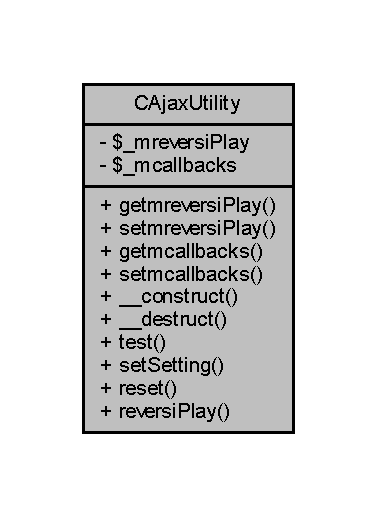
\includegraphics[width=181pt]{class_c_ajax_utility__coll__graph}
\end{center}
\end{figure}
\subsection*{Public Member Functions}
\begin{DoxyCompactItemize}
\item 
\mbox{\Hypertarget{class_c_ajax_utility_a3c233a6d5298f136e92700e6395070bc}\label{class_c_ajax_utility_a3c233a6d5298f136e92700e6395070bc}} 
{\bfseries getmreversi\+Play} ()
\item 
\mbox{\Hypertarget{class_c_ajax_utility_a05d77b59d799214fa7b4be00f10e99ba}\label{class_c_ajax_utility_a05d77b59d799214fa7b4be00f10e99ba}} 
{\bfseries setmreversi\+Play} (\$\+\_\+mreversi\+Play)
\item 
\mbox{\Hypertarget{class_c_ajax_utility_a4709b99adfa26d2049a3c68ef1ff3e0d}\label{class_c_ajax_utility_a4709b99adfa26d2049a3c68ef1ff3e0d}} 
{\bfseries getmcallbacks} ()
\item 
\mbox{\Hypertarget{class_c_ajax_utility_a8dd6bf96070e0b79942dc5fc0d52004c}\label{class_c_ajax_utility_a8dd6bf96070e0b79942dc5fc0d52004c}} 
{\bfseries setmcallbacks} (\$\+\_\+mcallbacks)
\item 
\hyperlink{class_c_ajax_utility_a095c5d389db211932136b53f25f39685}{\+\_\+\+\_\+construct} ()
\begin{DoxyCompactList}\small\item\em コンストラクタ \end{DoxyCompactList}\item 
\hyperlink{class_c_ajax_utility_a421831a265621325e1fdd19aace0c758}{\+\_\+\+\_\+destruct} ()
\begin{DoxyCompactList}\small\item\em デストラクタ \end{DoxyCompactList}\item 
\hyperlink{class_c_ajax_utility_ad69dd4607977cae05ebe19d1ae604fb1}{test} ()
\begin{DoxyCompactList}\small\item\em Ajaxテスト \end{DoxyCompactList}\item 
\hyperlink{class_c_ajax_utility_aeac0165d3e235a9aed9d1d5e9eec9f9c}{set\+Setting} (\$data)
\begin{DoxyCompactList}\small\item\em 設定反映 \end{DoxyCompactList}\item 
\hyperlink{class_c_ajax_utility_a4a20559544fdf4dcb457e258dc976cf8}{reset} ()
\begin{DoxyCompactList}\small\item\em リセット \end{DoxyCompactList}\item 
\hyperlink{class_c_ajax_utility_a017d2d85f7c5c6917f528f30452d72d0}{reversi\+Play} (\$y, \$x)
\begin{DoxyCompactList}\small\item\em リバーシプレイ \end{DoxyCompactList}\end{DoxyCompactItemize}
\subsection*{Private Attributes}
\begin{DoxyCompactItemize}
\item 
\mbox{\Hypertarget{class_c_ajax_utility_a2fdd2d2fbdbbba0dcd580cddf288b52e}\label{class_c_ajax_utility_a2fdd2d2fbdbbba0dcd580cddf288b52e}} 
\hyperlink{class_c_ajax_utility_a2fdd2d2fbdbbba0dcd580cddf288b52e}{\$\+\_\+mreversi\+Play}
\begin{DoxyCompactList}\small\item\em マスの状態 \end{DoxyCompactList}\item 
\mbox{\Hypertarget{class_c_ajax_utility_a384148a010c9db0531ea492d63bd4887}\label{class_c_ajax_utility_a384148a010c9db0531ea492d63bd4887}} 
\hyperlink{class_c_ajax_utility_a384148a010c9db0531ea492d63bd4887}{\$\+\_\+mcallbacks}
\begin{DoxyCompactList}\small\item\em コールバック \end{DoxyCompactList}\end{DoxyCompactItemize}


\subsection{Detailed Description}
Ajax\+Utlityクラス 

Definition at line 212 of file index.\+php.



\subsection{Constructor \& Destructor Documentation}
\mbox{\Hypertarget{class_c_ajax_utility_a095c5d389db211932136b53f25f39685}\label{class_c_ajax_utility_a095c5d389db211932136b53f25f39685}} 
\index{C\+Ajax\+Utility@{C\+Ajax\+Utility}!\+\_\+\+\_\+construct@{\+\_\+\+\_\+construct}}
\index{\+\_\+\+\_\+construct@{\+\_\+\+\_\+construct}!C\+Ajax\+Utility@{C\+Ajax\+Utility}}
\subsubsection{\texorpdfstring{\+\_\+\+\_\+construct()}{\_\_construct()}}
{\footnotesize\ttfamily \+\_\+\+\_\+construct (\begin{DoxyParamCaption}{ }\end{DoxyParamCaption})}



コンストラクタ 

\begin{DoxyReturn}{Returns}
ありません 
\end{DoxyReturn}
\begin{DoxyAuthor}{Author}
Yuta Yoshinaga 
\end{DoxyAuthor}
\begin{DoxyDate}{Date}
2018.\+03.\+02 
\end{DoxyDate}


Definition at line 231 of file index.\+php.

\mbox{\Hypertarget{class_c_ajax_utility_a421831a265621325e1fdd19aace0c758}\label{class_c_ajax_utility_a421831a265621325e1fdd19aace0c758}} 
\index{C\+Ajax\+Utility@{C\+Ajax\+Utility}!\+\_\+\+\_\+destruct@{\+\_\+\+\_\+destruct}}
\index{\+\_\+\+\_\+destruct@{\+\_\+\+\_\+destruct}!C\+Ajax\+Utility@{C\+Ajax\+Utility}}
\subsubsection{\texorpdfstring{\+\_\+\+\_\+destruct()}{\_\_destruct()}}
{\footnotesize\ttfamily \+\_\+\+\_\+destruct (\begin{DoxyParamCaption}{ }\end{DoxyParamCaption})}



デストラクタ 

\begin{DoxyReturn}{Returns}
ありません 
\end{DoxyReturn}
\begin{DoxyAuthor}{Author}
Yuta Yoshinaga 
\end{DoxyAuthor}
\begin{DoxyDate}{Date}
2018.\+03.\+02 
\end{DoxyDate}


Definition at line 241 of file index.\+php.



\subsection{Member Function Documentation}
\mbox{\Hypertarget{class_c_ajax_utility_a4a20559544fdf4dcb457e258dc976cf8}\label{class_c_ajax_utility_a4a20559544fdf4dcb457e258dc976cf8}} 
\index{C\+Ajax\+Utility@{C\+Ajax\+Utility}!reset@{reset}}
\index{reset@{reset}!C\+Ajax\+Utility@{C\+Ajax\+Utility}}
\subsubsection{\texorpdfstring{reset()}{reset()}}
{\footnotesize\ttfamily reset (\begin{DoxyParamCaption}{ }\end{DoxyParamCaption})}



リセット 

\begin{DoxyReturn}{Returns}
実行結果json 
\end{DoxyReturn}
\begin{DoxyAuthor}{Author}
Yuta Yoshinaga 
\end{DoxyAuthor}
\begin{DoxyDate}{Date}
2018.\+03.\+02 
\end{DoxyDate}


Definition at line 304 of file index.\+php.

\mbox{\Hypertarget{class_c_ajax_utility_a017d2d85f7c5c6917f528f30452d72d0}\label{class_c_ajax_utility_a017d2d85f7c5c6917f528f30452d72d0}} 
\index{C\+Ajax\+Utility@{C\+Ajax\+Utility}!reversi\+Play@{reversi\+Play}}
\index{reversi\+Play@{reversi\+Play}!C\+Ajax\+Utility@{C\+Ajax\+Utility}}
\subsubsection{\texorpdfstring{reversi\+Play()}{reversiPlay()}}
{\footnotesize\ttfamily reversi\+Play (\begin{DoxyParamCaption}\item[{}]{\$y,  }\item[{}]{\$x }\end{DoxyParamCaption})}



リバーシプレイ 


\begin{DoxyParams}[1]{Parameters}
\mbox{\tt in}  & {\em \$y} & \$y座標 \\
\hline
\mbox{\tt in}  & {\em \$x} & \$x座標 \\
\hline
\end{DoxyParams}
\begin{DoxyReturn}{Returns}
実行結果json 
\end{DoxyReturn}
\begin{DoxyAuthor}{Author}
Yuta Yoshinaga 
\end{DoxyAuthor}
\begin{DoxyDate}{Date}
2018.\+03.\+02 
\end{DoxyDate}


Definition at line 328 of file index.\+php.

\mbox{\Hypertarget{class_c_ajax_utility_aeac0165d3e235a9aed9d1d5e9eec9f9c}\label{class_c_ajax_utility_aeac0165d3e235a9aed9d1d5e9eec9f9c}} 
\index{C\+Ajax\+Utility@{C\+Ajax\+Utility}!set\+Setting@{set\+Setting}}
\index{set\+Setting@{set\+Setting}!C\+Ajax\+Utility@{C\+Ajax\+Utility}}
\subsubsection{\texorpdfstring{set\+Setting()}{setSetting()}}
{\footnotesize\ttfamily set\+Setting (\begin{DoxyParamCaption}\item[{}]{\$data }\end{DoxyParamCaption})}



設定反映 


\begin{DoxyParams}[1]{Parameters}
\mbox{\tt in}  & {\em \$data} & 設定データ(連想配列形式) \\
\hline
\end{DoxyParams}
\begin{DoxyReturn}{Returns}
実行結果json 
\end{DoxyReturn}
\begin{DoxyAuthor}{Author}
Yuta Yoshinaga 
\end{DoxyAuthor}
\begin{DoxyDate}{Date}
2018.\+03.\+02 
\end{DoxyDate}


Definition at line 262 of file index.\+php.

\mbox{\Hypertarget{class_c_ajax_utility_ad69dd4607977cae05ebe19d1ae604fb1}\label{class_c_ajax_utility_ad69dd4607977cae05ebe19d1ae604fb1}} 
\index{C\+Ajax\+Utility@{C\+Ajax\+Utility}!test@{test}}
\index{test@{test}!C\+Ajax\+Utility@{C\+Ajax\+Utility}}
\subsubsection{\texorpdfstring{test()}{test()}}
{\footnotesize\ttfamily test (\begin{DoxyParamCaption}{ }\end{DoxyParamCaption})}



Ajaxテスト 

\begin{DoxyReturn}{Returns}
ありません 
\end{DoxyReturn}
\begin{DoxyAuthor}{Author}
Yuta Yoshinaga 
\end{DoxyAuthor}
\begin{DoxyDate}{Date}
2018.\+03.\+02 
\end{DoxyDate}


Definition at line 251 of file index.\+php.



The documentation for this class was generated from the following file\+:\begin{DoxyCompactItemize}
\item 
Controller/\hyperlink{index_8php}{index.\+php}\end{DoxyCompactItemize}

\hypertarget{class_dbug_l}{}\section{DbugL Class Reference}
\label{class_dbug_l}\index{DbugL@{DbugL}}


Collaboration diagram for DbugL\+:
\nopagebreak
\begin{figure}[H]
\begin{center}
\leavevmode
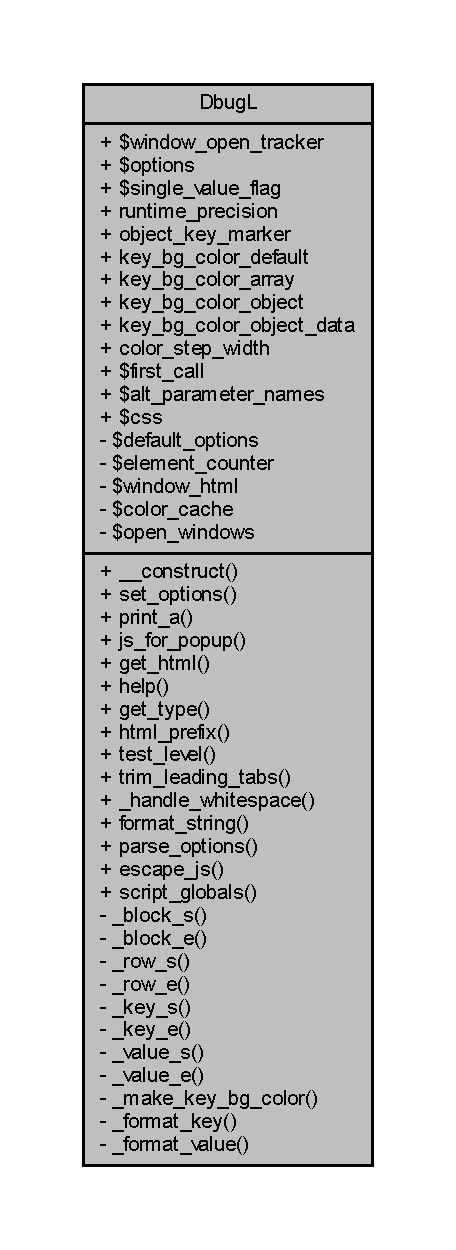
\includegraphics[height=550pt]{class_dbug_l__coll__graph}
\end{center}
\end{figure}
\subsection*{Public Member Functions}
\begin{DoxyCompactItemize}
\item 
\mbox{\Hypertarget{class_dbug_l_a519f2c0532394498c7f363731960f4de}\label{class_dbug_l_a519f2c0532394498c7f363731960f4de}} 
{\bfseries set\+\_\+options} (\$options\+\_\+string)
\item 
\mbox{\Hypertarget{class_dbug_l_a5ef54a81e7a97043bd7b964a31e5ecf5}\label{class_dbug_l_a5ef54a81e7a97043bd7b964a31e5ecf5}} 
{\bfseries print\+\_\+a} (\$input, \&\$html, \$iter=0)
\item 
\mbox{\Hypertarget{class_dbug_l_ab2156df9e320e1a85d9ce6cdedb687cd}\label{class_dbug_l_ab2156df9e320e1a85d9ce6cdedb687cd}} 
{\bfseries js\+\_\+for\+\_\+popup} (\$html)
\item 
\mbox{\Hypertarget{class_dbug_l_a264917dc38c1b88283ca308cb607a98a}\label{class_dbug_l_a264917dc38c1b88283ca308cb607a98a}} 
{\bfseries get\+\_\+html} (\$html)
\end{DoxyCompactItemize}
\subsection*{Static Public Member Functions}
\begin{DoxyCompactItemize}
\item 
\mbox{\Hypertarget{class_dbug_l_a88c15ce9c2420dbe752efa546669b84e}\label{class_dbug_l_a88c15ce9c2420dbe752efa546669b84e}} 
static {\bfseries help} (\$return\+\_\+mode=F\+A\+L\+SE)
\item 
\mbox{\Hypertarget{class_dbug_l_a4819d3a1c3b36e520cf801d8397fb3ec}\label{class_dbug_l_a4819d3a1c3b36e520cf801d8397fb3ec}} 
static {\bfseries get\+\_\+type} (\$value)
\item 
\mbox{\Hypertarget{class_dbug_l_a4c9298c3172427d7bc48994b27c921d5}\label{class_dbug_l_a4c9298c3172427d7bc48994b27c921d5}} 
static {\bfseries html\+\_\+prefix} ()
\item 
\mbox{\Hypertarget{class_dbug_l_a0f251fc06b9095331952439f4c3819a2}\label{class_dbug_l_a0f251fc06b9095331952439f4c3819a2}} 
static {\bfseries test\+\_\+level} (\$level)
\item 
\mbox{\Hypertarget{class_dbug_l_ab8f150beb454f23fed7204f944a6d134}\label{class_dbug_l_ab8f150beb454f23fed7204f944a6d134}} 
static {\bfseries trim\+\_\+leading\+\_\+tabs} ( \$string, \$tab\+\_\+padding=N\+U\+LL)
\item 
\mbox{\Hypertarget{class_dbug_l_a20c16e3deec26ba6be22a969ae1df10d}\label{class_dbug_l_a20c16e3deec26ba6be22a969ae1df10d}} 
static {\bfseries \+\_\+handle\+\_\+whitespace} ( \$string)
\item 
\mbox{\Hypertarget{class_dbug_l_affee7edb640cab947fb7e34dafb2e593}\label{class_dbug_l_affee7edb640cab947fb7e34dafb2e593}} 
static {\bfseries format\+\_\+string} (\$string, \$trim\+\_\+tabs=N\+U\+LL, \$escape\+\_\+html=2)
\item 
\mbox{\Hypertarget{class_dbug_l_a4d000b2c863d7c9c384ecaa7f5249f62}\label{class_dbug_l_a4d000b2c863d7c9c384ecaa7f5249f62}} 
static {\bfseries parse\+\_\+options} (\$options\+\_\+string=N\+U\+LL, \$alt\+\_\+parameter\+\_\+names=array())
\item 
\mbox{\Hypertarget{class_dbug_l_a78bbbd22db141177702aafe36e5a6c4f}\label{class_dbug_l_a78bbbd22db141177702aafe36e5a6c4f}} 
static {\bfseries escape\+\_\+js} (\$string)
\item 
\mbox{\Hypertarget{class_dbug_l_ae93bc61c2c69d06c6ac7e16c9f5017ee}\label{class_dbug_l_ae93bc61c2c69d06c6ac7e16c9f5017ee}} 
static {\bfseries script\+\_\+globals} ()
\end{DoxyCompactItemize}
\subsection*{Data Fields}
\begin{DoxyCompactItemize}
\item 
\mbox{\Hypertarget{class_dbug_l_ac97e4fac24ade158e91acf313dd8a155}\label{class_dbug_l_ac97e4fac24ade158e91acf313dd8a155}} 
{\bfseries \$window\+\_\+open\+\_\+tracker} = array()
\item 
\mbox{\Hypertarget{class_dbug_l_a011800c63ece4cbbfa77136a20607023}\label{class_dbug_l_a011800c63ece4cbbfa77136a20607023}} 
{\bfseries \$options} = array()
\item 
\mbox{\Hypertarget{class_dbug_l_ad3fb20899a2279c7de28dc2ee908f7db}\label{class_dbug_l_ad3fb20899a2279c7de28dc2ee908f7db}} 
{\bfseries \$single\+\_\+value\+\_\+flag} = F\+A\+L\+SE
\item 
\mbox{\Hypertarget{class_dbug_l_aecb99deaead9e8ade9b0ec994992cfe4}\label{class_dbug_l_aecb99deaead9e8ade9b0ec994992cfe4}} 
const {\bfseries runtime\+\_\+precision} = 6
\item 
\mbox{\Hypertarget{class_dbug_l_a1119f5dcc6e5189e0411d9e4b7f80dd0}\label{class_dbug_l_a1119f5dcc6e5189e0411d9e4b7f80dd0}} 
const {\bfseries object\+\_\+key\+\_\+marker} = \textquotesingle{}$<$\+:$\sim$!O\+B\+J\+E\+C\+T\+\_\+\+K\+E\+Y!$\sim$\+:$>$\textquotesingle{}
\item 
\mbox{\Hypertarget{class_dbug_l_aa97b017d454064a95dd08fbec7bf5f6f}\label{class_dbug_l_aa97b017d454064a95dd08fbec7bf5f6f}} 
const {\bfseries key\+\_\+bg\+\_\+color\+\_\+default} = \textquotesingle{}00456\+A\textquotesingle{}
\item 
\mbox{\Hypertarget{class_dbug_l_a0c40e80b5a47f7358c7bf9a2459ce5e2}\label{class_dbug_l_a0c40e80b5a47f7358c7bf9a2459ce5e2}} 
const {\bfseries key\+\_\+bg\+\_\+color\+\_\+array} = \textquotesingle{}10187\+E\textquotesingle{}
\item 
\mbox{\Hypertarget{class_dbug_l_a82f9deea9c5b770dfd19211792cec4b2}\label{class_dbug_l_a82f9deea9c5b770dfd19211792cec4b2}} 
const {\bfseries key\+\_\+bg\+\_\+color\+\_\+object} = \textquotesingle{}60008\+F\textquotesingle{}
\item 
\mbox{\Hypertarget{class_dbug_l_ab41675023cb1eee3a91b276a8ae294d5}\label{class_dbug_l_ab41675023cb1eee3a91b276a8ae294d5}} 
const {\bfseries key\+\_\+bg\+\_\+color\+\_\+object\+\_\+data} = \textquotesingle{}60008\+F\textquotesingle{}
\item 
\mbox{\Hypertarget{class_dbug_l_a22ff5a7c0075ac8e3daf381a966a8314}\label{class_dbug_l_a22ff5a7c0075ac8e3daf381a966a8314}} 
const {\bfseries color\+\_\+step\+\_\+width} = 10
\end{DoxyCompactItemize}
\subsection*{Static Public Attributes}
\begin{DoxyCompactItemize}
\item 
\mbox{\Hypertarget{class_dbug_l_a04ee1aab6042607d0db5516909872b56}\label{class_dbug_l_a04ee1aab6042607d0db5516909872b56}} 
static {\bfseries \$first\+\_\+call} = T\+R\+UE
\item 
static {\bfseries \$alt\+\_\+parameter\+\_\+names}
\item 
\mbox{\Hypertarget{class_dbug_l_a5619065f778cf71da2d43cbc4c47a1c4}\label{class_dbug_l_a5619065f778cf71da2d43cbc4c47a1c4}} 
static {\bfseries \$css}
\end{DoxyCompactItemize}
\subsection*{Private Member Functions}
\begin{DoxyCompactItemize}
\item 
\mbox{\Hypertarget{class_dbug_l_a7e72eb9c84f4f0c2fe153642ddb4c4f9}\label{class_dbug_l_a7e72eb9c84f4f0c2fe153642ddb4c4f9}} 
{\bfseries \+\_\+block\+\_\+s} (\$class=\textquotesingle{}null\textquotesingle{}, \$title=N\+U\+LL)
\item 
\mbox{\Hypertarget{class_dbug_l_af6a70d7736e478b5c3b01f82adac0ac9}\label{class_dbug_l_af6a70d7736e478b5c3b01f82adac0ac9}} 
{\bfseries \+\_\+block\+\_\+e} ()
\item 
\mbox{\Hypertarget{class_dbug_l_a06667e93215f834f8caf4db67678551e}\label{class_dbug_l_a06667e93215f834f8caf4db67678551e}} 
{\bfseries \+\_\+row\+\_\+s} (\$class=\textquotesingle{}null\textquotesingle{})
\item 
\mbox{\Hypertarget{class_dbug_l_a51663c177f44acbec564fd8698bd372f}\label{class_dbug_l_a51663c177f44acbec564fd8698bd372f}} 
{\bfseries \+\_\+row\+\_\+e} ()
\item 
\mbox{\Hypertarget{class_dbug_l_aeb1c15638f05146cf5d46abbff827e75}\label{class_dbug_l_aeb1c15638f05146cf5d46abbff827e75}} 
{\bfseries \+\_\+key\+\_\+s} (\$bg\+\_\+color, \$class, \$value)
\item 
\mbox{\Hypertarget{class_dbug_l_ae1339a1e78cf0fc0953f0ed88addcf35}\label{class_dbug_l_ae1339a1e78cf0fc0953f0ed88addcf35}} 
{\bfseries \+\_\+key\+\_\+e} ()
\item 
\mbox{\Hypertarget{class_dbug_l_abf8a67721334e3a2fd32d5263e58b5af}\label{class_dbug_l_abf8a67721334e3a2fd32d5263e58b5af}} 
{\bfseries \+\_\+value\+\_\+s} (\$class=\textquotesingle{}null\textquotesingle{})
\item 
\mbox{\Hypertarget{class_dbug_l_a975dbf588381f78cef42c7262a0bf6c2}\label{class_dbug_l_a975dbf588381f78cef42c7262a0bf6c2}} 
{\bfseries \+\_\+value\+\_\+e} ()
\item 
\mbox{\Hypertarget{class_dbug_l_a97f268ad4d27f45c8c3ec48c2f444abf}\label{class_dbug_l_a97f268ad4d27f45c8c3ec48c2f444abf}} 
{\bfseries \+\_\+make\+\_\+key\+\_\+bg\+\_\+color} (\$base\+\_\+color, \$iter)
\item 
\mbox{\Hypertarget{class_dbug_l_a06297e9e2b6689ac28defc11a5adee7d}\label{class_dbug_l_a06297e9e2b6689ac28defc11a5adee7d}} 
{\bfseries \+\_\+format\+\_\+key} (\$key, \$value, \$iter, \$special\+\_\+type=N\+U\+LL)
\item 
\mbox{\Hypertarget{class_dbug_l_a749b00eebbe81490001a3e0c3e551225}\label{class_dbug_l_a749b00eebbe81490001a3e0c3e551225}} 
{\bfseries \+\_\+format\+\_\+value} (\$value)
\end{DoxyCompactItemize}
\subsection*{Private Attributes}
\begin{DoxyCompactItemize}
\item 
{\bfseries \$default\+\_\+options}
\item 
\mbox{\Hypertarget{class_dbug_l_af3143168826ba263bb690477bab0f447}\label{class_dbug_l_af3143168826ba263bb690477bab0f447}} 
{\bfseries \$element\+\_\+counter} = 0
\item 
\mbox{\Hypertarget{class_dbug_l_a6cd18782a86fd3da0fd3dafb37d110cf}\label{class_dbug_l_a6cd18782a86fd3da0fd3dafb37d110cf}} 
{\bfseries \$window\+\_\+html}
\item 
\mbox{\Hypertarget{class_dbug_l_a85c749b87c66e24e852d61cda3dcb8a6}\label{class_dbug_l_a85c749b87c66e24e852d61cda3dcb8a6}} 
{\bfseries \$color\+\_\+cache} = array()
\item 
\mbox{\Hypertarget{class_dbug_l_ad53f539453e86a108680c38e084ed9ea}\label{class_dbug_l_ad53f539453e86a108680c38e084ed9ea}} 
{\bfseries \$open\+\_\+windows} = array()
\end{DoxyCompactItemize}


\subsection{Detailed Description}


Definition at line 64 of file debuglib.\+php.



\subsection{Field Documentation}
\mbox{\Hypertarget{class_dbug_l_adf653966d88d3be577d68ba39936722c}\label{class_dbug_l_adf653966d88d3be577d68ba39936722c}} 
\index{DbugL@{DbugL}!\$alt\+\_\+parameter\+\_\+names@{\$alt\+\_\+parameter\+\_\+names}}
\index{\$alt\+\_\+parameter\+\_\+names@{\$alt\+\_\+parameter\+\_\+names}!DbugL@{DbugL}}
\subsubsection{\texorpdfstring{\$alt\+\_\+parameter\+\_\+names}{$alt\_parameter\_names}}
{\footnotesize\ttfamily \$alt\+\_\+parameter\+\_\+names\hspace{0.3cm}{\ttfamily [static]}}

{\bfseries Initial value\+:}
\begin{DoxyCode}
= array(
            \textcolor{stringliteral}{'trim\_tabs'}    => array(\textcolor{stringliteral}{'tt'}),
            \textcolor{stringliteral}{'label'}        => array(\textcolor{charliteral}{'l'}),
            \textcolor{stringliteral}{'max\_y'}        => array(\textcolor{charliteral}{'y'}),
            \textcolor{stringliteral}{'return'}       => array(\textcolor{charliteral}{'r'}),
            \textcolor{stringliteral}{'window'}       => array(\textcolor{charliteral}{'w'}),
            \textcolor{stringliteral}{'window\_link'}  => array(\textcolor{stringliteral}{'wl'}),
            \textcolor{stringliteral}{'debug\_level'}  => array(\textcolor{stringliteral}{'lvl'}),
            \textcolor{stringliteral}{'show\_objects'} => array(\textcolor{stringliteral}{'so'}),
            \textcolor{stringliteral}{'pickle'}       => array(\textcolor{charliteral}{'p'}),
            \textcolor{stringliteral}{'mail'}         => array(\textcolor{charliteral}{'m'}),
            \textcolor{stringliteral}{'mail\_encoding'}=> array(\textcolor{stringliteral}{'me'}),
            \textcolor{stringliteral}{'escape\_html'}  => array(\textcolor{charliteral}{'e'}),
        )
\end{DoxyCode}


Definition at line 69 of file debuglib.\+php.

\mbox{\Hypertarget{class_dbug_l_adcc21e090cb7801165d93287bb63c117}\label{class_dbug_l_adcc21e090cb7801165d93287bb63c117}} 
\index{DbugL@{DbugL}!\$default\+\_\+options@{\$default\+\_\+options}}
\index{\$default\+\_\+options@{\$default\+\_\+options}!DbugL@{DbugL}}
\subsubsection{\texorpdfstring{\$default\+\_\+options}{$default\_options}}
{\footnotesize\ttfamily \$default\+\_\+options\hspace{0.3cm}{\ttfamily [private]}}

{\bfseries Initial value\+:}
\begin{DoxyCode}
= array(
            \textcolor{stringliteral}{'label'}               => NULL,
            \textcolor{stringliteral}{'window'}              => NULL,
            \textcolor{stringliteral}{'window\_link'}         => FALSE,
            \textcolor{stringliteral}{'max\_y'}               => 0,
            \textcolor{stringliteral}{'test\_for\_recursions'} => FALSE,
            \textcolor{stringliteral}{'show\_objects'}        => TRUE,
            \textcolor{stringliteral}{'trim\_tabs'}           => NULL,
            \textcolor{stringliteral}{'avoid@'}              => FALSE,
            \textcolor{stringliteral}{'return'}              => FALSE,
            \textcolor{stringliteral}{'pickle'}              => FALSE,
            \textcolor{stringliteral}{'export'}              => FALSE,
            \textcolor{stringliteral}{'escape\_html'}         => 2,
            \textcolor{stringliteral}{'mail'}                => NULL,
            \textcolor{stringliteral}{'mail\_encoding'}       => \textcolor{stringliteral}{'utf-8'}, 
            \textcolor{stringliteral}{'debug\_level'}         => 0,
        )
\end{DoxyCode}


Definition at line 197 of file debuglib.\+php.



The documentation for this class was generated from the following file\+:\begin{DoxyCompactItemize}
\item 
debuglib.\+php\end{DoxyCompactItemize}

\hypertarget{class_delegate}{}\section{Delegate Class Reference}
\label{class_delegate}\index{Delegate@{Delegate}}


Collaboration diagram for Delegate\+:
\nopagebreak
\begin{figure}[H]
\begin{center}
\leavevmode
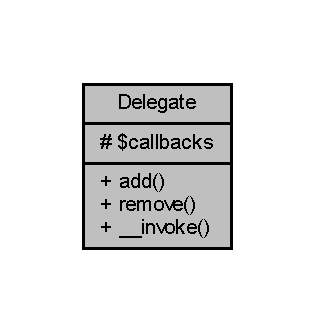
\includegraphics[width=151pt]{class_delegate__coll__graph}
\end{center}
\end{figure}
\subsection*{Public Member Functions}
\begin{DoxyCompactItemize}
\item 
\hyperlink{class_delegate_a2db8611725175f0ef569cb2ee7d1ef24}{add} (callable \$callback)
\item 
\hyperlink{class_delegate_aba650b6c889c96ddacd660d1e4e1a1d7}{remove} (callable \$callback)
\item 
\hyperlink{class_delegate_a9aac7e1475efe923de4e19cc2511f092}{\+\_\+\+\_\+invoke} ()
\end{DoxyCompactItemize}
\subsection*{Protected Attributes}
\begin{DoxyCompactItemize}
\item 
\mbox{\Hypertarget{class_delegate_a151f6e603ac02a25364ad54bee36ab2a}\label{class_delegate_a151f6e603ac02a25364ad54bee36ab2a}} 
{\bfseries \$callbacks} = \mbox{[}$\,$\mbox{]}
\end{DoxyCompactItemize}


\subsection{Detailed Description}


Definition at line 20 of file Delegate.\+php.



\subsection{Member Function Documentation}
\mbox{\Hypertarget{class_delegate_a9aac7e1475efe923de4e19cc2511f092}\label{class_delegate_a9aac7e1475efe923de4e19cc2511f092}} 
\index{Delegate@{Delegate}!\+\_\+\+\_\+invoke@{\+\_\+\+\_\+invoke}}
\index{\+\_\+\+\_\+invoke@{\+\_\+\+\_\+invoke}!Delegate@{Delegate}}
\subsubsection{\texorpdfstring{\+\_\+\+\_\+invoke()}{\_\_invoke()}}
{\footnotesize\ttfamily \+\_\+\+\_\+invoke (\begin{DoxyParamCaption}{ }\end{DoxyParamCaption})}

Invoke callback functions \begin{DoxyReturn}{Returns}
mixed 
\end{DoxyReturn}


Definition at line 58 of file Delegate.\+php.

\mbox{\Hypertarget{class_delegate_a2db8611725175f0ef569cb2ee7d1ef24}\label{class_delegate_a2db8611725175f0ef569cb2ee7d1ef24}} 
\index{Delegate@{Delegate}!add@{add}}
\index{add@{add}!Delegate@{Delegate}}
\subsubsection{\texorpdfstring{add()}{add()}}
{\footnotesize\ttfamily add (\begin{DoxyParamCaption}\item[{callable}]{\$callback }\end{DoxyParamCaption})}

Add callback function 
\begin{DoxyParams}[1]{Parameters}
callable & {\em \$callback} & \\
\hline
\end{DoxyParams}
\begin{DoxyReturn}{Returns}
\$this 
\end{DoxyReturn}


Definition at line 30 of file Delegate.\+php.

\mbox{\Hypertarget{class_delegate_aba650b6c889c96ddacd660d1e4e1a1d7}\label{class_delegate_aba650b6c889c96ddacd660d1e4e1a1d7}} 
\index{Delegate@{Delegate}!remove@{remove}}
\index{remove@{remove}!Delegate@{Delegate}}
\subsubsection{\texorpdfstring{remove()}{remove()}}
{\footnotesize\ttfamily remove (\begin{DoxyParamCaption}\item[{callable}]{\$callback }\end{DoxyParamCaption})}

Remove callback function 
\begin{DoxyParams}[1]{Parameters}
callable & {\em \$callback} & \\
\hline
\end{DoxyParams}
\begin{DoxyReturn}{Returns}
\$this 
\end{DoxyReturn}


Definition at line 41 of file Delegate.\+php.



The documentation for this class was generated from the following file\+:\begin{DoxyCompactItemize}
\item 
Model/\hyperlink{_delegate_8php}{Delegate.\+php}\end{DoxyCompactItemize}

\hypertarget{class_reversi}{}\section{Reversi Class Reference}
\label{class_reversi}\index{Reversi@{Reversi}}


リバーシクラス  




Collaboration diagram for Reversi\+:\nopagebreak
\begin{figure}[H]
\begin{center}
\leavevmode
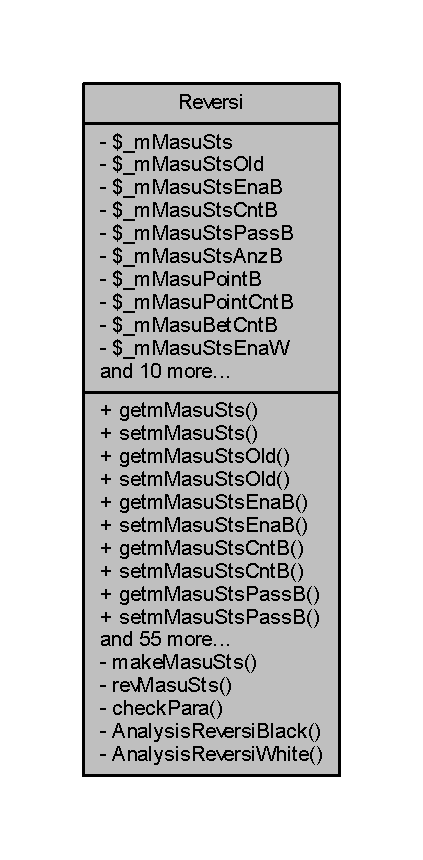
\includegraphics[width=203pt]{class_reversi__coll__graph}
\end{center}
\end{figure}
\subsection*{Public Member Functions}
\begin{DoxyCompactItemize}
\item 
\mbox{\Hypertarget{class_reversi_a995fd4e134f3161d0d67caddd362ddda}\label{class_reversi_a995fd4e134f3161d0d67caddd362ddda}} 
{\bfseries getm\+Masu\+Sts} ()
\item 
\mbox{\Hypertarget{class_reversi_abfd5a55ea9efdd26a609557b59c0d12e}\label{class_reversi_abfd5a55ea9efdd26a609557b59c0d12e}} 
{\bfseries setm\+Masu\+Sts} (\$\+\_\+m\+Masu\+Sts)
\item 
\mbox{\Hypertarget{class_reversi_a32328d1f1bf56d2e84141a8c9804f359}\label{class_reversi_a32328d1f1bf56d2e84141a8c9804f359}} 
{\bfseries getm\+Masu\+Sts\+Old} ()
\item 
\mbox{\Hypertarget{class_reversi_a71900505df416c91732e8e0196127b94}\label{class_reversi_a71900505df416c91732e8e0196127b94}} 
{\bfseries setm\+Masu\+Sts\+Old} (\$\+\_\+m\+Masu\+Sts\+Old)
\item 
\mbox{\Hypertarget{class_reversi_aff36ab36553b866ca2a8be3fdf3bf2f0}\label{class_reversi_aff36ab36553b866ca2a8be3fdf3bf2f0}} 
{\bfseries getm\+Masu\+Sts\+EnaB} ()
\item 
\mbox{\Hypertarget{class_reversi_a96a62c362d81a5861eb5e875de2376f0}\label{class_reversi_a96a62c362d81a5861eb5e875de2376f0}} 
{\bfseries setm\+Masu\+Sts\+EnaB} (\$\+\_\+m\+Masu\+Sts\+EnaB)
\item 
\mbox{\Hypertarget{class_reversi_ae26e602c710657395eb489795fd0ccb7}\label{class_reversi_ae26e602c710657395eb489795fd0ccb7}} 
{\bfseries getm\+Masu\+Sts\+CntB} ()
\item 
\mbox{\Hypertarget{class_reversi_a006a77defc43d4195d30950666710e7d}\label{class_reversi_a006a77defc43d4195d30950666710e7d}} 
{\bfseries setm\+Masu\+Sts\+CntB} (\$\+\_\+m\+Masu\+Sts\+CntB)
\item 
\mbox{\Hypertarget{class_reversi_afc5e8bfd7ef5cfa8d4b93ab0146b1bd6}\label{class_reversi_afc5e8bfd7ef5cfa8d4b93ab0146b1bd6}} 
{\bfseries getm\+Masu\+Sts\+PassB} ()
\item 
\mbox{\Hypertarget{class_reversi_a426ce5e0ef8cd875b75abe23c0d14a14}\label{class_reversi_a426ce5e0ef8cd875b75abe23c0d14a14}} 
{\bfseries setm\+Masu\+Sts\+PassB} (\$\+\_\+m\+Masu\+Sts\+PassB)
\item 
\mbox{\Hypertarget{class_reversi_aba5dc09ce4db9c40e13575e5b10f3ea7}\label{class_reversi_aba5dc09ce4db9c40e13575e5b10f3ea7}} 
{\bfseries getm\+Masu\+Sts\+AnzB} ()
\item 
\mbox{\Hypertarget{class_reversi_ab95634419bbdec6708972b4364a1f7b4}\label{class_reversi_ab95634419bbdec6708972b4364a1f7b4}} 
{\bfseries setm\+Masu\+Sts\+AnzB} (\$\+\_\+m\+Masu\+Sts\+AnzB)
\item 
\mbox{\Hypertarget{class_reversi_a6d5b9c28b3a92e01b42ed862985d2f98}\label{class_reversi_a6d5b9c28b3a92e01b42ed862985d2f98}} 
{\bfseries getm\+Masu\+PointB} ()
\item 
\mbox{\Hypertarget{class_reversi_ae4fa18aa71c2e6d5c2faed6719bff776}\label{class_reversi_ae4fa18aa71c2e6d5c2faed6719bff776}} 
{\bfseries setm\+Masu\+PointB} (\$\+\_\+m\+Masu\+PointB)
\item 
\mbox{\Hypertarget{class_reversi_ae75baf790b7d8b4892f6a2e0f0eb8e67}\label{class_reversi_ae75baf790b7d8b4892f6a2e0f0eb8e67}} 
{\bfseries getm\+Masu\+Point\+CntB} ()
\item 
\mbox{\Hypertarget{class_reversi_a78f0479c5fa03a015ac9ec6492e05c4f}\label{class_reversi_a78f0479c5fa03a015ac9ec6492e05c4f}} 
{\bfseries setm\+Masu\+Point\+CntB} (\$\+\_\+m\+Masu\+Point\+CntB)
\item 
\mbox{\Hypertarget{class_reversi_aa0883ee24e29449c6bb89d161521ed67}\label{class_reversi_aa0883ee24e29449c6bb89d161521ed67}} 
{\bfseries getm\+Masu\+Bet\+CntB} ()
\item 
\mbox{\Hypertarget{class_reversi_a6243772dbdb1bbe38c01f908457d5743}\label{class_reversi_a6243772dbdb1bbe38c01f908457d5743}} 
{\bfseries setm\+Masu\+Bet\+CntB} (\$\+\_\+m\+Masu\+Bet\+CntB)
\item 
\mbox{\Hypertarget{class_reversi_aefef308965d0fe90daf393d4b0a04184}\label{class_reversi_aefef308965d0fe90daf393d4b0a04184}} 
{\bfseries getm\+Masu\+Sts\+EnaW} ()
\item 
\mbox{\Hypertarget{class_reversi_a230f00edf5b575f24a7094d18123fe4a}\label{class_reversi_a230f00edf5b575f24a7094d18123fe4a}} 
{\bfseries setm\+Masu\+Sts\+EnaW} (\$\+\_\+m\+Masu\+Sts\+EnaW)
\item 
\mbox{\Hypertarget{class_reversi_a04067fac0467af0e096cb3115fa804f4}\label{class_reversi_a04067fac0467af0e096cb3115fa804f4}} 
{\bfseries getm\+Masu\+Sts\+CntW} ()
\item 
\mbox{\Hypertarget{class_reversi_a112112f495910acedc8ec201fa669ae3}\label{class_reversi_a112112f495910acedc8ec201fa669ae3}} 
{\bfseries setm\+Masu\+Sts\+CntW} (\$\+\_\+m\+Masu\+Sts\+CntW)
\item 
\mbox{\Hypertarget{class_reversi_a51598ce2b9166a720cf2f9de321c00eb}\label{class_reversi_a51598ce2b9166a720cf2f9de321c00eb}} 
{\bfseries getm\+Masu\+Sts\+PassW} ()
\item 
\mbox{\Hypertarget{class_reversi_a76f39ccd1a55c6202985c310af21448d}\label{class_reversi_a76f39ccd1a55c6202985c310af21448d}} 
{\bfseries setm\+Masu\+Sts\+PassW} (\$\+\_\+m\+Masu\+Sts\+PassW)
\item 
\mbox{\Hypertarget{class_reversi_a2e6dc6afd4e1f554a3a314e2638dc5aa}\label{class_reversi_a2e6dc6afd4e1f554a3a314e2638dc5aa}} 
{\bfseries getm\+Masu\+Sts\+AnzW} ()
\item 
\mbox{\Hypertarget{class_reversi_a2fa42edd87104a0048ca0efecbb59708}\label{class_reversi_a2fa42edd87104a0048ca0efecbb59708}} 
{\bfseries setm\+Masu\+Sts\+AnzW} (\$\+\_\+m\+Masu\+Sts\+AnzW)
\item 
\mbox{\Hypertarget{class_reversi_ad8037037ea6c12c5f72bb1d1b5802d98}\label{class_reversi_ad8037037ea6c12c5f72bb1d1b5802d98}} 
{\bfseries getm\+Masu\+PointW} ()
\item 
\mbox{\Hypertarget{class_reversi_a216f8ea81ed1a4d567bcbb9efe03b358}\label{class_reversi_a216f8ea81ed1a4d567bcbb9efe03b358}} 
{\bfseries setm\+Masu\+PointW} (\$\+\_\+m\+Masu\+PointW)
\item 
\mbox{\Hypertarget{class_reversi_aa34fdde67253d92780a746ab64371956}\label{class_reversi_aa34fdde67253d92780a746ab64371956}} 
{\bfseries getm\+Masu\+Point\+CntW} ()
\item 
\mbox{\Hypertarget{class_reversi_ab0ec543b38c99910b3f4b254c757b9b3}\label{class_reversi_ab0ec543b38c99910b3f4b254c757b9b3}} 
{\bfseries setm\+Masu\+Point\+CntW} (\$\+\_\+m\+Masu\+Point\+CntW)
\item 
\mbox{\Hypertarget{class_reversi_a513ff1271786bb02da384150ee891453}\label{class_reversi_a513ff1271786bb02da384150ee891453}} 
{\bfseries getm\+Masu\+Bet\+CntW} ()
\item 
\mbox{\Hypertarget{class_reversi_ae2b4be273c04556474b686db886cc97b}\label{class_reversi_ae2b4be273c04556474b686db886cc97b}} 
{\bfseries setm\+Masu\+Bet\+CntW} (\$\+\_\+m\+Masu\+Bet\+CntW)
\item 
\mbox{\Hypertarget{class_reversi_a6ce2cf2d07330bbca1ca6e48557fd777}\label{class_reversi_a6ce2cf2d07330bbca1ca6e48557fd777}} 
{\bfseries getm\+Masu\+Sts\+EnaL} ()
\item 
\mbox{\Hypertarget{class_reversi_aa014d804f4eae9d38d7f807e362f1abc}\label{class_reversi_aa014d804f4eae9d38d7f807e362f1abc}} 
{\bfseries setm\+Masu\+Sts\+EnaL} (\$\+\_\+m\+Masu\+Sts\+EnaL)
\item 
\mbox{\Hypertarget{class_reversi_a58f70e77c23b8a4460dc0065ac44fbcd}\label{class_reversi_a58f70e77c23b8a4460dc0065ac44fbcd}} 
{\bfseries getm\+Masu\+Sts\+CntL} ()
\item 
\mbox{\Hypertarget{class_reversi_a6a504f963054c7931d021ef63f99b86e}\label{class_reversi_a6a504f963054c7931d021ef63f99b86e}} 
{\bfseries setm\+Masu\+Sts\+CntL} (\$\+\_\+m\+Masu\+Sts\+CntL)
\item 
\mbox{\Hypertarget{class_reversi_a3f9ad087f95c8e5f31ef050e63c89247}\label{class_reversi_a3f9ad087f95c8e5f31ef050e63c89247}} 
{\bfseries getm\+Masu\+Sts\+PassL} ()
\item 
\mbox{\Hypertarget{class_reversi_a3a4da0cd20c0b5dfca9be0815601ccc5}\label{class_reversi_a3a4da0cd20c0b5dfca9be0815601ccc5}} 
{\bfseries setm\+Masu\+Sts\+PassL} (\$\+\_\+m\+Masu\+Sts\+PassL)
\item 
\mbox{\Hypertarget{class_reversi_a5d376e79bf04bb31b383db61b151bcdb}\label{class_reversi_a5d376e79bf04bb31b383db61b151bcdb}} 
{\bfseries getm\+Masu\+Sts\+AnzL} ()
\item 
\mbox{\Hypertarget{class_reversi_a36b350417fa59ab47a67c00c4accf938}\label{class_reversi_a36b350417fa59ab47a67c00c4accf938}} 
{\bfseries setm\+Masu\+Sts\+AnzL} (\$\+\_\+m\+Masu\+Sts\+AnzL)
\item 
\mbox{\Hypertarget{class_reversi_ade5dc108155b6e6f6395154438720b93}\label{class_reversi_ade5dc108155b6e6f6395154438720b93}} 
{\bfseries getm\+Masu\+PointL} ()
\item 
\mbox{\Hypertarget{class_reversi_ad9bd42936ec274c9fa618cc8ece556cd}\label{class_reversi_ad9bd42936ec274c9fa618cc8ece556cd}} 
{\bfseries setm\+Masu\+PointL} (\$\+\_\+m\+Masu\+PointL)
\item 
\mbox{\Hypertarget{class_reversi_a25055af3ec722a3825942a9926a444fa}\label{class_reversi_a25055af3ec722a3825942a9926a444fa}} 
{\bfseries getm\+Masu\+Point\+CntL} ()
\item 
\mbox{\Hypertarget{class_reversi_a5087882e3eb4cf95cade4af6b3dba950}\label{class_reversi_a5087882e3eb4cf95cade4af6b3dba950}} 
{\bfseries setm\+Masu\+Point\+CntL} (\$\+\_\+m\+Masu\+Point\+CntL)
\item 
\mbox{\Hypertarget{class_reversi_a62cbae970465838c48134d8776bc9fce}\label{class_reversi_a62cbae970465838c48134d8776bc9fce}} 
{\bfseries getm\+Masu\+Bet\+CntL} ()
\item 
\mbox{\Hypertarget{class_reversi_a5ef49272f519ffeec78b4a40a838703c}\label{class_reversi_a5ef49272f519ffeec78b4a40a838703c}} 
{\bfseries setm\+Masu\+Bet\+CntL} (\$\+\_\+m\+Masu\+Bet\+CntL)
\item 
\mbox{\Hypertarget{class_reversi_a400f08e1bdbfbd48883c7ad9bcd980f2}\label{class_reversi_a400f08e1bdbfbd48883c7ad9bcd980f2}} 
{\bfseries getm\+Masu\+Sts\+EnaR} ()
\item 
\mbox{\Hypertarget{class_reversi_a12de5517d872db381e89d318c2a75e6d}\label{class_reversi_a12de5517d872db381e89d318c2a75e6d}} 
{\bfseries setm\+Masu\+Sts\+EnaR} (\$\+\_\+m\+Masu\+Sts\+EnaR)
\item 
\mbox{\Hypertarget{class_reversi_a370ffeac2b210aebf1f5b371bc00d7c9}\label{class_reversi_a370ffeac2b210aebf1f5b371bc00d7c9}} 
{\bfseries getm\+Masu\+Sts\+CntR} ()
\item 
\mbox{\Hypertarget{class_reversi_a9ca61ff195b34e438add6692f41a6386}\label{class_reversi_a9ca61ff195b34e438add6692f41a6386}} 
{\bfseries setm\+Masu\+Sts\+CntR} (\$\+\_\+m\+Masu\+Sts\+CntR)
\item 
\mbox{\Hypertarget{class_reversi_a2ec5a89484fd5c286448ff5a884c1632}\label{class_reversi_a2ec5a89484fd5c286448ff5a884c1632}} 
{\bfseries getm\+Masu\+Sts\+PassR} ()
\item 
\mbox{\Hypertarget{class_reversi_aac545fa9b9ab9b67fe82df20cf8407f6}\label{class_reversi_aac545fa9b9ab9b67fe82df20cf8407f6}} 
{\bfseries setm\+Masu\+Sts\+PassR} (\$\+\_\+m\+Masu\+Sts\+PassR)
\item 
\mbox{\Hypertarget{class_reversi_aa1079d1b51766bf3fc3f9b07b6576fd4}\label{class_reversi_aa1079d1b51766bf3fc3f9b07b6576fd4}} 
{\bfseries getm\+Masu\+Sts\+AnzR} ()
\item 
\mbox{\Hypertarget{class_reversi_abb23a9169bf5234ad622727aacb9c1c9}\label{class_reversi_abb23a9169bf5234ad622727aacb9c1c9}} 
{\bfseries setm\+Masu\+Sts\+AnzR} (\$\+\_\+m\+Masu\+Sts\+AnzR)
\item 
\mbox{\Hypertarget{class_reversi_a0ca54cdec65e33e2bbaef3ec87753c71}\label{class_reversi_a0ca54cdec65e33e2bbaef3ec87753c71}} 
{\bfseries getm\+Masu\+PointR} ()
\item 
\mbox{\Hypertarget{class_reversi_a07d115546600aa6b50ea911b6d007aa2}\label{class_reversi_a07d115546600aa6b50ea911b6d007aa2}} 
{\bfseries setm\+Masu\+PointR} (\$\+\_\+m\+Masu\+PointR)
\item 
\mbox{\Hypertarget{class_reversi_ae59671198100c6d1042e592c238bcf98}\label{class_reversi_ae59671198100c6d1042e592c238bcf98}} 
{\bfseries getm\+Masu\+Point\+CntR} ()
\item 
\mbox{\Hypertarget{class_reversi_aaf5eb7b8a9e6c579641091965b98403c}\label{class_reversi_aaf5eb7b8a9e6c579641091965b98403c}} 
{\bfseries setm\+Masu\+Point\+CntR} (\$\+\_\+m\+Masu\+Point\+CntR)
\item 
\mbox{\Hypertarget{class_reversi_abb1a37c4605dd7eae7db5c1e1d49ca2f}\label{class_reversi_abb1a37c4605dd7eae7db5c1e1d49ca2f}} 
{\bfseries getm\+Masu\+Bet\+CntR} ()
\item 
\mbox{\Hypertarget{class_reversi_aed1c77174f806e8459c288d2818da914}\label{class_reversi_aed1c77174f806e8459c288d2818da914}} 
{\bfseries setm\+Masu\+Bet\+CntR} (\$\+\_\+m\+Masu\+Bet\+CntR)
\item 
\mbox{\Hypertarget{class_reversi_a32cebf699f9aa19d9053c143c3562d3a}\label{class_reversi_a32cebf699f9aa19d9053c143c3562d3a}} 
{\bfseries getm\+Masu\+Cnt} ()
\item 
\mbox{\Hypertarget{class_reversi_ad50e5fa90e6a2f53bf71ed04bed603ae}\label{class_reversi_ad50e5fa90e6a2f53bf71ed04bed603ae}} 
{\bfseries setm\+Masu\+Cnt} (\$\+\_\+m\+Masu\+Cnt)
\item 
\mbox{\Hypertarget{class_reversi_a3ac7b23d1b6567faa4d58d51a952c859}\label{class_reversi_a3ac7b23d1b6567faa4d58d51a952c859}} 
{\bfseries getm\+Masu\+Cnt\+Max} ()
\item 
\mbox{\Hypertarget{class_reversi_ae2dbd35c16269ab04a58aba0194f7faf}\label{class_reversi_ae2dbd35c16269ab04a58aba0194f7faf}} 
{\bfseries setm\+Masu\+Cnt\+Max} (\$\+\_\+m\+Masu\+Cnt\+Max)
\item 
\mbox{\Hypertarget{class_reversi_a577b674fea2b90470da3217b5390fe9c}\label{class_reversi_a577b674fea2b90470da3217b5390fe9c}} 
{\bfseries getm\+Masu\+Hist\+Cur} ()
\item 
\mbox{\Hypertarget{class_reversi_a827554ef8aeb4c252bf4690c709ef762}\label{class_reversi_a827554ef8aeb4c252bf4690c709ef762}} 
{\bfseries setm\+Masu\+Hist\+Cur} (\$\+\_\+m\+Masu\+Hist\+Cur)
\item 
\mbox{\Hypertarget{class_reversi_a0eb2a30637500aef9245d2f82f68b769}\label{class_reversi_a0eb2a30637500aef9245d2f82f68b769}} 
{\bfseries getm\+Masu\+Hist} ()
\item 
\mbox{\Hypertarget{class_reversi_a26300550a0cc4f665b32426907b8ff0d}\label{class_reversi_a26300550a0cc4f665b32426907b8ff0d}} 
{\bfseries setm\+Masu\+Hist} (\$\+\_\+m\+Masu\+Hist)
\item 
\hyperlink{class_reversi_a6667ca490c75777ec233f3ead04c5fd7}{\+\_\+\+\_\+construct} (\$masu\+Cnt, \$masu\+Max)
\begin{DoxyCompactList}\small\item\em コンストラクタ \end{DoxyCompactList}\item 
\hyperlink{class_reversi_a421831a265621325e1fdd19aace0c758}{\+\_\+\+\_\+destruct} ()
\begin{DoxyCompactList}\small\item\em デストラクタ \end{DoxyCompactList}\item 
\hyperlink{class_reversi_a4a20559544fdf4dcb457e258dc976cf8}{reset} ()
\begin{DoxyCompactList}\small\item\em リセット \end{DoxyCompactList}\item 
\hyperlink{class_reversi_a1e2f4c432c1e407c4dbec20f4ee1b3b7}{Analysis\+Reversi} (\$b\+Pass\+Ena, \$w\+Pass\+Ena, \$l\+Pass\+Ena, \$r\+Pass\+Ena)
\begin{DoxyCompactList}\small\item\em 解析を行う \end{DoxyCompactList}\item 
\hyperlink{class_reversi_a1baed538e7a503cd51850d368b9e65f7}{get\+Masu\+Sts} (\$y, \$x)
\begin{DoxyCompactList}\small\item\em マスステータスを取得 \end{DoxyCompactList}\item 
\hyperlink{class_reversi_a1688a929d3917e19510f6501c42d6a2b}{get\+Masu\+Sts\+Old} (\$y, \$x)
\begin{DoxyCompactList}\small\item\em 以前のマスステータスを取得 \end{DoxyCompactList}\item 
\hyperlink{class_reversi_a22088e18c7f837f49093595261c30e4e}{get\+Masu\+Sts\+Ena} (\$color, \$y, \$x)
\begin{DoxyCompactList}\small\item\em 指定座標に指定色を置けるかチェック \end{DoxyCompactList}\item 
\hyperlink{class_reversi_a10bfc13effc2db9a681a2906792be453}{get\+Masu\+Sts\+Cnt} (\$color, \$y, \$x)
\begin{DoxyCompactList}\small\item\em 指定座標の獲得コマ数取得 \end{DoxyCompactList}\item 
\hyperlink{class_reversi_aead5ee041feb6ac2609266614ea06f78}{get\+Color\+Ena} (\$color)
\begin{DoxyCompactList}\small\item\em 指定色が現在置ける場所があるかチェック \end{DoxyCompactList}\item 
\hyperlink{class_reversi_aab9985c789e464de6cf99d7d725cb5a3}{get\+Game\+End\+Sts} ()
\begin{DoxyCompactList}\small\item\em ゲーム終了かチェック \end{DoxyCompactList}\item 
\hyperlink{class_reversi_a26f3168c7d94e70d344841d65885a4ac}{set\+Masu\+Sts} (\$color, \$y, \$x)
\begin{DoxyCompactList}\small\item\em 指定座標にコマを置く \end{DoxyCompactList}\item 
\hyperlink{class_reversi_ae659a2ce33e395f8d5cda5e62d03fe7e}{set\+Masu\+Sts\+Forcibly} (\$color, \$y, \$x)
\begin{DoxyCompactList}\small\item\em 指定座標にコマを強制的に置く \end{DoxyCompactList}\item 
\hyperlink{class_reversi_ab6853cc0f53e50a70d576f15296f0864}{set\+Masu\+Cnt} (\$cnt)
\begin{DoxyCompactList}\small\item\em マスの数変更 \end{DoxyCompactList}\item 
\hyperlink{class_reversi_ad059cc09b0001edd980f43770380b863}{get\+Point} (\$color, \$num)
\begin{DoxyCompactList}\small\item\em ポイント座標取得 \end{DoxyCompactList}\item 
\hyperlink{class_reversi_af538d04718f177f71461f582f3bd8eba}{get\+Point\+Cnt} (\$color)
\begin{DoxyCompactList}\small\item\em ポイント座標数取得 \end{DoxyCompactList}\item 
\hyperlink{class_reversi_acb1491c467c3065beece256256f5f59d}{get\+Bet\+Cnt} (\$color)
\begin{DoxyCompactList}\small\item\em コマ数取得 \end{DoxyCompactList}\item 
\hyperlink{class_reversi_a123959981f8e1d48fc7b9d183a5c6d0a}{get\+Pass\+Ena} (\$color, \$y, \$x)
\begin{DoxyCompactList}\small\item\em パス判定 \end{DoxyCompactList}\item 
\hyperlink{class_reversi_a41cae82a798f2b3d0684bda44b837fcf}{get\+History} (\$num)
\begin{DoxyCompactList}\small\item\em 履歴取得 \end{DoxyCompactList}\item 
\hyperlink{class_reversi_a004834cf9f95ab56b62c1305bbc68ce2}{get\+History\+Cnt} ()
\begin{DoxyCompactList}\small\item\em 履歴数取得 \end{DoxyCompactList}\item 
\hyperlink{class_reversi_af1a30d438a7d17f31353b9d4bfe9cb65}{get\+Point\+Anz} (\$color, \$y, \$x)
\begin{DoxyCompactList}\small\item\em ポイント座標解析取得 \end{DoxyCompactList}\item 
\hyperlink{class_reversi_acd2c64ea43cc26407ad64920a183446b}{check\+Edge} (\$color, \$y, \$x)
\begin{DoxyCompactList}\small\item\em 角の隣に置いても角を取られないマス検索 \end{DoxyCompactList}\item 
\hyperlink{class_reversi_a76a7addedc2b0ba83c6b46ce0601076c}{get\+Edge\+Side\+Zero} (\$y, \$x)
\begin{DoxyCompactList}\small\item\em 指定座標が角か取得 \end{DoxyCompactList}\item 
\hyperlink{class_reversi_a98aff7f2db3a9feacbe98293c6b80eb4}{get\+Edge\+Side\+One} (\$y, \$x)
\begin{DoxyCompactList}\small\item\em 指定座標が角の一つ手前か取得 \end{DoxyCompactList}\item 
\hyperlink{class_reversi_a968982683aa41f50c83789a9be05aaba}{get\+Edge\+Side\+Two} (\$y, \$x)
\begin{DoxyCompactList}\small\item\em 指定座標が角の二つ手前か取得 \end{DoxyCompactList}\item 
\hyperlink{class_reversi_ab299d2488c8ab29f646e449d3204efbc}{get\+Edge\+Side\+Three} (\$y, \$x)
\begin{DoxyCompactList}\small\item\em 指定座標が角の三つ以上手前か取得 \end{DoxyCompactList}\end{DoxyCompactItemize}
\subsection*{Private Member Functions}
\begin{DoxyCompactItemize}
\item 
\hyperlink{class_reversi_a88869682786bb7c45c3488113deaa789}{make\+Masu\+Sts} (\$color)
\begin{DoxyCompactList}\small\item\em 各コマの置ける場所等のステータス作成 \end{DoxyCompactList}\item 
\hyperlink{class_reversi_af29cd3f41dc1cffead056dbbed55ae7a}{rev\+Masu\+Sts} (\$color, \$y, \$x)
\begin{DoxyCompactList}\small\item\em コマをひっくり返す \end{DoxyCompactList}\item 
\hyperlink{class_reversi_ac8d57b64bc839c8bb1f53a2a5db11228}{check\+Para} (\$para, \$min, \$max)
\begin{DoxyCompactList}\small\item\em パラメーター範囲チェック \end{DoxyCompactList}\item 
\hyperlink{class_reversi_a471972ec549188f7eb701d57e14ae7a1}{Analysis\+Reversi\+Black} ()
\begin{DoxyCompactList}\small\item\em 解析を行う(黒) \end{DoxyCompactList}\item 
\hyperlink{class_reversi_a3c30afb2509b0782b1c22a8770c68c48}{Analysis\+Reversi\+White} ()
\begin{DoxyCompactList}\small\item\em 解析を行う(白) \end{DoxyCompactList}\item 
\hyperlink{class_reversi_a3b581c4861bda72706a1d7146c910ad2}{Analysis\+Reversi\+Blue} ()
\begin{DoxyCompactList}\small\item\em 解析を行う(青) \end{DoxyCompactList}\item 
\hyperlink{class_reversi_ad44cfa7c45a98365df2d6db094d61901}{Analysis\+Reversi\+Red} ()
\begin{DoxyCompactList}\small\item\em 解析を行う(赤) \end{DoxyCompactList}\end{DoxyCompactItemize}
\subsection*{Private Attributes}
\begin{DoxyCompactItemize}
\item 
\mbox{\Hypertarget{class_reversi_a22a84a78f0a3b0f9931591298e2da4d7}\label{class_reversi_a22a84a78f0a3b0f9931591298e2da4d7}} 
\hyperlink{class_reversi_a22a84a78f0a3b0f9931591298e2da4d7}{\$\+\_\+m\+Masu\+Sts}
\begin{DoxyCompactList}\small\item\em マスの状態 \end{DoxyCompactList}\item 
\mbox{\Hypertarget{class_reversi_af7aec5a588ed3b17db84cd79c2e2599d}\label{class_reversi_af7aec5a588ed3b17db84cd79c2e2599d}} 
\hyperlink{class_reversi_af7aec5a588ed3b17db84cd79c2e2599d}{\$\+\_\+m\+Masu\+Sts\+Old}
\begin{DoxyCompactList}\small\item\em 以前のマスの状態 \end{DoxyCompactList}\item 
\mbox{\Hypertarget{class_reversi_a9fd66ba0b00c0bab1f84e64526653c38}\label{class_reversi_a9fd66ba0b00c0bab1f84e64526653c38}} 
\hyperlink{class_reversi_a9fd66ba0b00c0bab1f84e64526653c38}{\$\+\_\+m\+Masu\+Sts\+EnaB}
\begin{DoxyCompactList}\small\item\em 黒の置ける場所 \end{DoxyCompactList}\item 
\mbox{\Hypertarget{class_reversi_a24c5cf73681d3920c3330e9d0afaf3a2}\label{class_reversi_a24c5cf73681d3920c3330e9d0afaf3a2}} 
\hyperlink{class_reversi_a24c5cf73681d3920c3330e9d0afaf3a2}{\$\+\_\+m\+Masu\+Sts\+CntB}
\begin{DoxyCompactList}\small\item\em 黒の獲得コマ数 \end{DoxyCompactList}\item 
\mbox{\Hypertarget{class_reversi_a384407818dc2c9378716ee1f135b9f01}\label{class_reversi_a384407818dc2c9378716ee1f135b9f01}} 
\hyperlink{class_reversi_a384407818dc2c9378716ee1f135b9f01}{\$\+\_\+m\+Masu\+Sts\+PassB}
\begin{DoxyCompactList}\small\item\em 黒が相手をパスさせる場所 \end{DoxyCompactList}\item 
\mbox{\Hypertarget{class_reversi_ade4534b9cb287ab570e5cbd9c6b8099c}\label{class_reversi_ade4534b9cb287ab570e5cbd9c6b8099c}} 
\hyperlink{class_reversi_ade4534b9cb287ab570e5cbd9c6b8099c}{\$\+\_\+m\+Masu\+Sts\+AnzB}
\begin{DoxyCompactList}\small\item\em 黒がその場所に置いた場合の解析結果 \end{DoxyCompactList}\item 
\mbox{\Hypertarget{class_reversi_a015fefbe17d9d4f13946cecb89493e37}\label{class_reversi_a015fefbe17d9d4f13946cecb89493e37}} 
\hyperlink{class_reversi_a015fefbe17d9d4f13946cecb89493e37}{\$\+\_\+m\+Masu\+PointB}
\begin{DoxyCompactList}\small\item\em 黒の置ける場所座標一覧 \end{DoxyCompactList}\item 
\mbox{\Hypertarget{class_reversi_af8936304d7c1ccb26eb7343172e11987}\label{class_reversi_af8936304d7c1ccb26eb7343172e11987}} 
\hyperlink{class_reversi_af8936304d7c1ccb26eb7343172e11987}{\$\+\_\+m\+Masu\+Point\+CntB}
\begin{DoxyCompactList}\small\item\em 黒の置ける場所座標一覧数 \end{DoxyCompactList}\item 
\mbox{\Hypertarget{class_reversi_abf0e4db44b6b0ae1ecec4827e2394cdd}\label{class_reversi_abf0e4db44b6b0ae1ecec4827e2394cdd}} 
\hyperlink{class_reversi_abf0e4db44b6b0ae1ecec4827e2394cdd}{\$\+\_\+m\+Masu\+Bet\+CntB}
\begin{DoxyCompactList}\small\item\em 黒コマ数 \end{DoxyCompactList}\item 
\mbox{\Hypertarget{class_reversi_a1cf814c44538183769e091e84e4c810b}\label{class_reversi_a1cf814c44538183769e091e84e4c810b}} 
\hyperlink{class_reversi_a1cf814c44538183769e091e84e4c810b}{\$\+\_\+m\+Masu\+Sts\+EnaW}
\begin{DoxyCompactList}\small\item\em 白の置ける場所 \end{DoxyCompactList}\item 
\mbox{\Hypertarget{class_reversi_a14d7803befeac5ddaf9bedbac66e0812}\label{class_reversi_a14d7803befeac5ddaf9bedbac66e0812}} 
\hyperlink{class_reversi_a14d7803befeac5ddaf9bedbac66e0812}{\$\+\_\+m\+Masu\+Sts\+CntW}
\begin{DoxyCompactList}\small\item\em 白の獲得コマ数 \end{DoxyCompactList}\item 
\mbox{\Hypertarget{class_reversi_a3a60b04cc5f54e1196feffc0ec12d89a}\label{class_reversi_a3a60b04cc5f54e1196feffc0ec12d89a}} 
\hyperlink{class_reversi_a3a60b04cc5f54e1196feffc0ec12d89a}{\$\+\_\+m\+Masu\+Sts\+PassW}
\begin{DoxyCompactList}\small\item\em 白が相手をパスさせる場所 \end{DoxyCompactList}\item 
\mbox{\Hypertarget{class_reversi_a8654984ca1ca888a7e2b97e9a2d099aa}\label{class_reversi_a8654984ca1ca888a7e2b97e9a2d099aa}} 
\hyperlink{class_reversi_a8654984ca1ca888a7e2b97e9a2d099aa}{\$\+\_\+m\+Masu\+Sts\+AnzW}
\begin{DoxyCompactList}\small\item\em 白がその場所に置いた場合の解析結果 \end{DoxyCompactList}\item 
\mbox{\Hypertarget{class_reversi_ac6007e0a7a850c31c37eb55ea74746a7}\label{class_reversi_ac6007e0a7a850c31c37eb55ea74746a7}} 
\hyperlink{class_reversi_ac6007e0a7a850c31c37eb55ea74746a7}{\$\+\_\+m\+Masu\+PointW}
\begin{DoxyCompactList}\small\item\em 白の置ける場所座標一覧 \end{DoxyCompactList}\item 
\mbox{\Hypertarget{class_reversi_aad5f6baed07b96cd5d06e38fd66f1c36}\label{class_reversi_aad5f6baed07b96cd5d06e38fd66f1c36}} 
\hyperlink{class_reversi_aad5f6baed07b96cd5d06e38fd66f1c36}{\$\+\_\+m\+Masu\+Point\+CntW}
\begin{DoxyCompactList}\small\item\em 白の置ける場所座標一覧数 \end{DoxyCompactList}\item 
\mbox{\Hypertarget{class_reversi_a92a21ca9d4bad37593fea8b3d2be6981}\label{class_reversi_a92a21ca9d4bad37593fea8b3d2be6981}} 
\hyperlink{class_reversi_a92a21ca9d4bad37593fea8b3d2be6981}{\$\+\_\+m\+Masu\+Bet\+CntW}
\begin{DoxyCompactList}\small\item\em 白コマ数 \end{DoxyCompactList}\item 
\mbox{\Hypertarget{class_reversi_a32f836e2f108ab5165927f05cb50977b}\label{class_reversi_a32f836e2f108ab5165927f05cb50977b}} 
\hyperlink{class_reversi_a32f836e2f108ab5165927f05cb50977b}{\$\+\_\+m\+Masu\+Sts\+EnaL}
\begin{DoxyCompactList}\small\item\em 青の置ける場所 \end{DoxyCompactList}\item 
\mbox{\Hypertarget{class_reversi_a860ce7417213f610eba14e79c6715f83}\label{class_reversi_a860ce7417213f610eba14e79c6715f83}} 
\hyperlink{class_reversi_a860ce7417213f610eba14e79c6715f83}{\$\+\_\+m\+Masu\+Sts\+CntL}
\begin{DoxyCompactList}\small\item\em 青の獲得コマ数 \end{DoxyCompactList}\item 
\mbox{\Hypertarget{class_reversi_a6d98a68c97f554ad389ebf35db5351f0}\label{class_reversi_a6d98a68c97f554ad389ebf35db5351f0}} 
\hyperlink{class_reversi_a6d98a68c97f554ad389ebf35db5351f0}{\$\+\_\+m\+Masu\+Sts\+PassL}
\begin{DoxyCompactList}\small\item\em 青が相手をパスさせる場所 \end{DoxyCompactList}\item 
\mbox{\Hypertarget{class_reversi_a898f51c5935e6e14e5b4fe64287f9b2e}\label{class_reversi_a898f51c5935e6e14e5b4fe64287f9b2e}} 
\hyperlink{class_reversi_a898f51c5935e6e14e5b4fe64287f9b2e}{\$\+\_\+m\+Masu\+Sts\+AnzL}
\begin{DoxyCompactList}\small\item\em 青がその場所に置いた場合の解析結果 \end{DoxyCompactList}\item 
\mbox{\Hypertarget{class_reversi_afbb0c4e7e3e9974fd20727287e49d6ac}\label{class_reversi_afbb0c4e7e3e9974fd20727287e49d6ac}} 
\hyperlink{class_reversi_afbb0c4e7e3e9974fd20727287e49d6ac}{\$\+\_\+m\+Masu\+PointL}
\begin{DoxyCompactList}\small\item\em 青の置ける場所座標一覧 \end{DoxyCompactList}\item 
\mbox{\Hypertarget{class_reversi_a4953efeebd1948a6482816c2123329b9}\label{class_reversi_a4953efeebd1948a6482816c2123329b9}} 
\hyperlink{class_reversi_a4953efeebd1948a6482816c2123329b9}{\$\+\_\+m\+Masu\+Point\+CntL}
\begin{DoxyCompactList}\small\item\em 青の置ける場所座標一覧数 \end{DoxyCompactList}\item 
\mbox{\Hypertarget{class_reversi_a1d2faac7092989202db9180bf6dd9fab}\label{class_reversi_a1d2faac7092989202db9180bf6dd9fab}} 
\hyperlink{class_reversi_a1d2faac7092989202db9180bf6dd9fab}{\$\+\_\+m\+Masu\+Bet\+CntL}
\begin{DoxyCompactList}\small\item\em 青コマ数 \end{DoxyCompactList}\item 
\mbox{\Hypertarget{class_reversi_add672fd9b0fd19e1602bc5d4bb9b0d88}\label{class_reversi_add672fd9b0fd19e1602bc5d4bb9b0d88}} 
\hyperlink{class_reversi_add672fd9b0fd19e1602bc5d4bb9b0d88}{\$\+\_\+m\+Masu\+Sts\+EnaR}
\begin{DoxyCompactList}\small\item\em 赤の置ける場所 \end{DoxyCompactList}\item 
\mbox{\Hypertarget{class_reversi_a8ebfe1e25ad504b7655c01828631a155}\label{class_reversi_a8ebfe1e25ad504b7655c01828631a155}} 
\hyperlink{class_reversi_a8ebfe1e25ad504b7655c01828631a155}{\$\+\_\+m\+Masu\+Sts\+CntR}
\begin{DoxyCompactList}\small\item\em 赤の獲得コマ数 \end{DoxyCompactList}\item 
\mbox{\Hypertarget{class_reversi_ad409dead7b1f751bb9ba087ced8cadfc}\label{class_reversi_ad409dead7b1f751bb9ba087ced8cadfc}} 
\hyperlink{class_reversi_ad409dead7b1f751bb9ba087ced8cadfc}{\$\+\_\+m\+Masu\+Sts\+PassR}
\begin{DoxyCompactList}\small\item\em 赤が相手をパスさせる場所 \end{DoxyCompactList}\item 
\mbox{\Hypertarget{class_reversi_a63c3ec2a9250f18aeb3e881a5c8724b1}\label{class_reversi_a63c3ec2a9250f18aeb3e881a5c8724b1}} 
\hyperlink{class_reversi_a63c3ec2a9250f18aeb3e881a5c8724b1}{\$\+\_\+m\+Masu\+Sts\+AnzR}
\begin{DoxyCompactList}\small\item\em 赤がその場所に置いた場合の解析結果 \end{DoxyCompactList}\item 
\mbox{\Hypertarget{class_reversi_a99f18f7afe6e931d3e7925e23bf15918}\label{class_reversi_a99f18f7afe6e931d3e7925e23bf15918}} 
\hyperlink{class_reversi_a99f18f7afe6e931d3e7925e23bf15918}{\$\+\_\+m\+Masu\+PointR}
\begin{DoxyCompactList}\small\item\em 赤の置ける場所座標一覧 \end{DoxyCompactList}\item 
\mbox{\Hypertarget{class_reversi_acca482f972640097ce9e343eacf4b35b}\label{class_reversi_acca482f972640097ce9e343eacf4b35b}} 
\hyperlink{class_reversi_acca482f972640097ce9e343eacf4b35b}{\$\+\_\+m\+Masu\+Point\+CntR}
\begin{DoxyCompactList}\small\item\em 赤の置ける場所座標一覧数 \end{DoxyCompactList}\item 
\mbox{\Hypertarget{class_reversi_a2fa15ed849e65338bbd900a09080c70b}\label{class_reversi_a2fa15ed849e65338bbd900a09080c70b}} 
\hyperlink{class_reversi_a2fa15ed849e65338bbd900a09080c70b}{\$\+\_\+m\+Masu\+Bet\+CntR}
\begin{DoxyCompactList}\small\item\em 赤コマ数 \end{DoxyCompactList}\item 
\mbox{\Hypertarget{class_reversi_a8ac63bcef31cc4d29b244456c62677bc}\label{class_reversi_a8ac63bcef31cc4d29b244456c62677bc}} 
\hyperlink{class_reversi_a8ac63bcef31cc4d29b244456c62677bc}{\$\+\_\+m\+Masu\+Cnt}
\begin{DoxyCompactList}\small\item\em 縦横マス数 \end{DoxyCompactList}\item 
\mbox{\Hypertarget{class_reversi_ae40f5163a8835d2ee564386a09ce196a}\label{class_reversi_ae40f5163a8835d2ee564386a09ce196a}} 
\hyperlink{class_reversi_ae40f5163a8835d2ee564386a09ce196a}{\$\+\_\+m\+Masu\+Cnt\+Max}
\begin{DoxyCompactList}\small\item\em 縦横マス最大数 \end{DoxyCompactList}\item 
\mbox{\Hypertarget{class_reversi_af77c253cf42f9796e0bdc729e6d0c087}\label{class_reversi_af77c253cf42f9796e0bdc729e6d0c087}} 
\hyperlink{class_reversi_af77c253cf42f9796e0bdc729e6d0c087}{\$\+\_\+m\+Masu\+Hist\+Cur}
\begin{DoxyCompactList}\small\item\em 履歴現在位置 \end{DoxyCompactList}\item 
\mbox{\Hypertarget{class_reversi_ad5e2d002bf79a6295aea9513cb11f2e3}\label{class_reversi_ad5e2d002bf79a6295aea9513cb11f2e3}} 
\hyperlink{class_reversi_ad5e2d002bf79a6295aea9513cb11f2e3}{\$\+\_\+m\+Masu\+Hist}
\begin{DoxyCompactList}\small\item\em 履歴 \end{DoxyCompactList}\end{DoxyCompactItemize}


\subsection{Detailed Description}
リバーシクラス 

Definition at line 30 of file Reversi.\+php.



\subsection{Constructor \& Destructor Documentation}
\mbox{\Hypertarget{class_reversi_a6667ca490c75777ec233f3ead04c5fd7}\label{class_reversi_a6667ca490c75777ec233f3ead04c5fd7}} 
\index{Reversi@{Reversi}!\+\_\+\+\_\+construct@{\+\_\+\+\_\+construct}}
\index{\+\_\+\+\_\+construct@{\+\_\+\+\_\+construct}!Reversi@{Reversi}}
\subsubsection{\texorpdfstring{\+\_\+\+\_\+construct()}{\_\_construct()}}
{\footnotesize\ttfamily \+\_\+\+\_\+construct (\begin{DoxyParamCaption}\item[{}]{\$masu\+Cnt,  }\item[{}]{\$masu\+Max }\end{DoxyParamCaption})}



コンストラクタ 


\begin{DoxyParams}[1]{Parameters}
\mbox{\tt in}  & {\em \$masu\+Cnt} & 縦横マス数 \\
\hline
\mbox{\tt in}  & {\em \$masu\+Max} & 縦横マス最大数 \\
\hline
\end{DoxyParams}
\begin{DoxyReturn}{Returns}
ありません 
\end{DoxyReturn}
\begin{DoxyAuthor}{Author}
Yuta Yoshinaga 
\end{DoxyAuthor}
\begin{DoxyDate}{Date}
2018.\+03.\+02 
\end{DoxyDate}


Definition at line 183 of file Reversi.\+php.

Here is the call graph for this function\+:\nopagebreak
\begin{figure}[H]
\begin{center}
\leavevmode
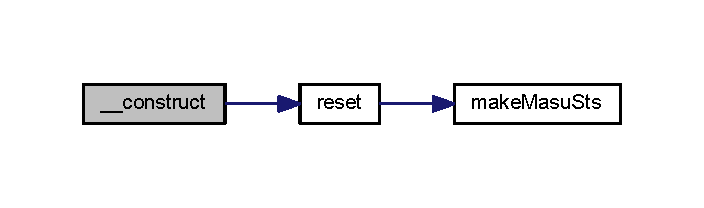
\includegraphics[width=338pt]{class_reversi_a6667ca490c75777ec233f3ead04c5fd7_cgraph}
\end{center}
\end{figure}
\mbox{\Hypertarget{class_reversi_a421831a265621325e1fdd19aace0c758}\label{class_reversi_a421831a265621325e1fdd19aace0c758}} 
\index{Reversi@{Reversi}!\+\_\+\+\_\+destruct@{\+\_\+\+\_\+destruct}}
\index{\+\_\+\+\_\+destruct@{\+\_\+\+\_\+destruct}!Reversi@{Reversi}}
\subsubsection{\texorpdfstring{\+\_\+\+\_\+destruct()}{\_\_destruct()}}
{\footnotesize\ttfamily \+\_\+\+\_\+destruct (\begin{DoxyParamCaption}{ }\end{DoxyParamCaption})}



デストラクタ 

\begin{DoxyReturn}{Returns}
ありません 
\end{DoxyReturn}
\begin{DoxyAuthor}{Author}
Yuta Yoshinaga 
\end{DoxyAuthor}
\begin{DoxyDate}{Date}
2018.\+03.\+02 
\end{DoxyDate}


Definition at line 294 of file Reversi.\+php.



\subsection{Member Function Documentation}
\mbox{\Hypertarget{class_reversi_a1e2f4c432c1e407c4dbec20f4ee1b3b7}\label{class_reversi_a1e2f4c432c1e407c4dbec20f4ee1b3b7}} 
\index{Reversi@{Reversi}!Analysis\+Reversi@{Analysis\+Reversi}}
\index{Analysis\+Reversi@{Analysis\+Reversi}!Reversi@{Reversi}}
\subsubsection{\texorpdfstring{Analysis\+Reversi()}{AnalysisReversi()}}
{\footnotesize\ttfamily void Analysis\+Reversi (\begin{DoxyParamCaption}\item[{}]{\$b\+Pass\+Ena,  }\item[{}]{\$w\+Pass\+Ena,  }\item[{}]{\$l\+Pass\+Ena,  }\item[{}]{\$r\+Pass\+Ena }\end{DoxyParamCaption})}



解析を行う 


\begin{DoxyParams}[1]{Parameters}
\mbox{\tt in}  & {\em \$b\+Pass\+Ena} & 1=黒パス有効 \\
\hline
\mbox{\tt in}  & {\em \$w\+Pass\+Ena} & 1=白パス有効 \\
\hline
\mbox{\tt in}  & {\em \$l\+Pass\+Ena} & 1=青パス有効 \\
\hline
\mbox{\tt in}  & {\em \$r\+Pass\+Ena} & 1=赤パス有効 \\
\hline
\end{DoxyParams}
\begin{DoxyReturn}{Returns}
ありません 
\end{DoxyReturn}
\begin{DoxyAuthor}{Author}
Yuta Yoshinaga 
\end{DoxyAuthor}
\begin{DoxyDate}{Date}
2018.\+03.\+02 
\end{DoxyDate}


Definition at line 1430 of file Reversi.\+php.

Here is the call graph for this function\+:\nopagebreak
\begin{figure}[H]
\begin{center}
\leavevmode
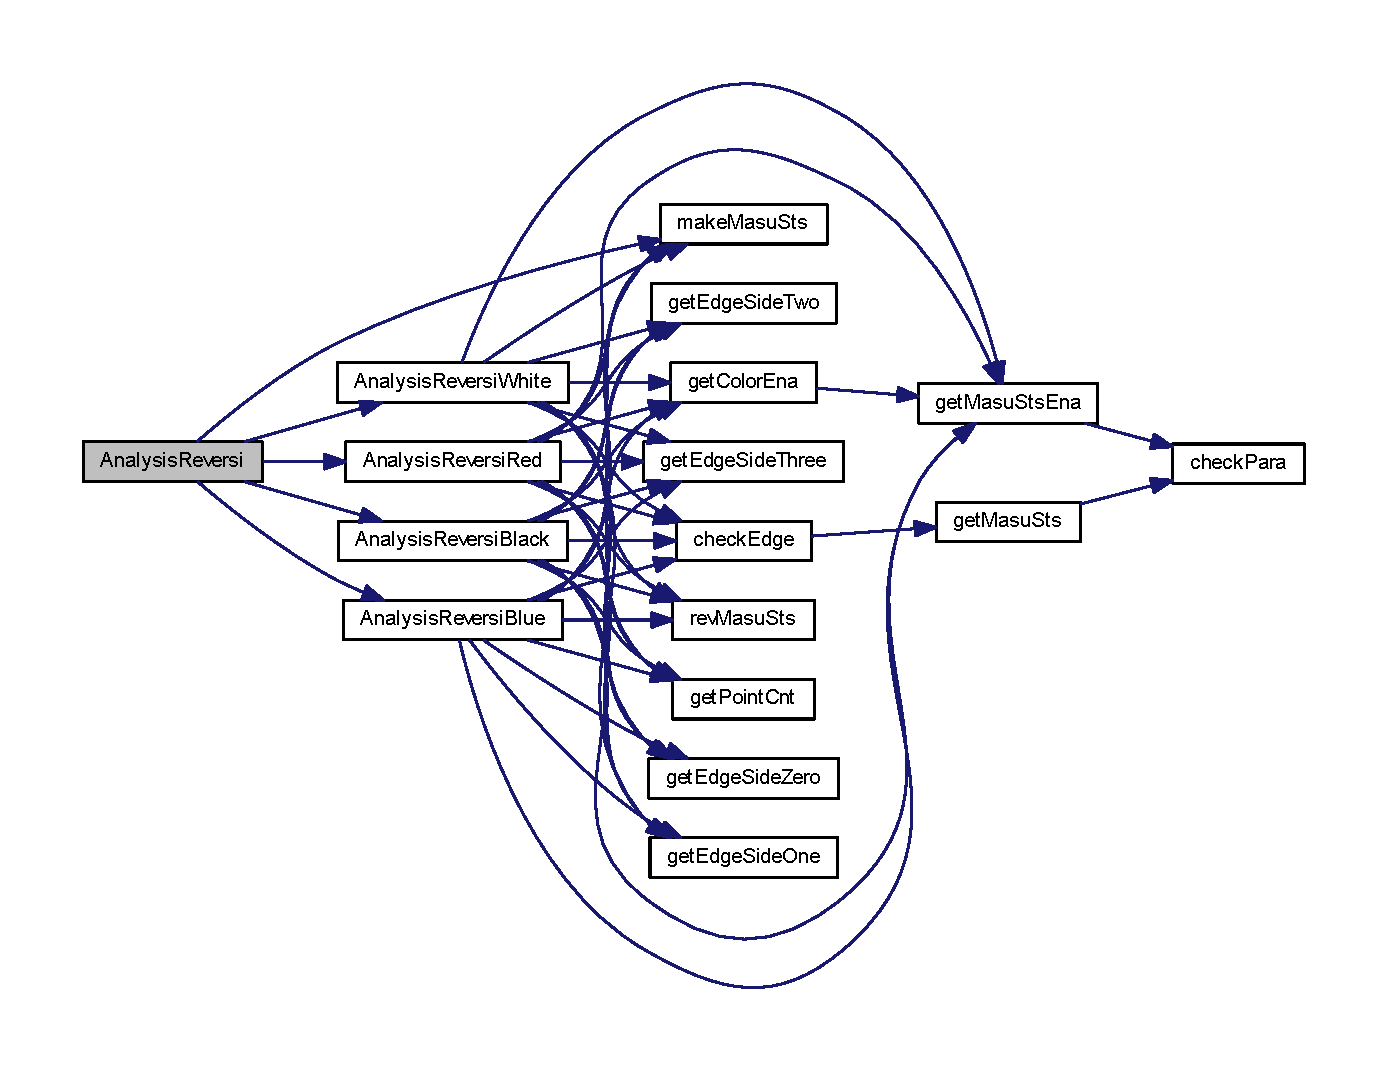
\includegraphics[width=350pt]{class_reversi_a1e2f4c432c1e407c4dbec20f4ee1b3b7_cgraph}
\end{center}
\end{figure}
\mbox{\Hypertarget{class_reversi_a471972ec549188f7eb701d57e14ae7a1}\label{class_reversi_a471972ec549188f7eb701d57e14ae7a1}} 
\index{Reversi@{Reversi}!Analysis\+Reversi\+Black@{Analysis\+Reversi\+Black}}
\index{Analysis\+Reversi\+Black@{Analysis\+Reversi\+Black}!Reversi@{Reversi}}
\subsubsection{\texorpdfstring{Analysis\+Reversi\+Black()}{AnalysisReversiBlack()}}
{\footnotesize\ttfamily Analysis\+Reversi\+Black (\begin{DoxyParamCaption}{ }\end{DoxyParamCaption})\hspace{0.3cm}{\ttfamily [private]}}



解析を行う(黒) 

\begin{DoxyReturn}{Returns}
ありません 
\end{DoxyReturn}
\begin{DoxyAuthor}{Author}
Yuta Yoshinaga 
\end{DoxyAuthor}
\begin{DoxyDate}{Date}
2018.\+03.\+02 
\end{DoxyDate}


Definition at line 798 of file Reversi.\+php.



Referenced by Analysis\+Reversi().

Here is the call graph for this function\+:\nopagebreak
\begin{figure}[H]
\begin{center}
\leavevmode
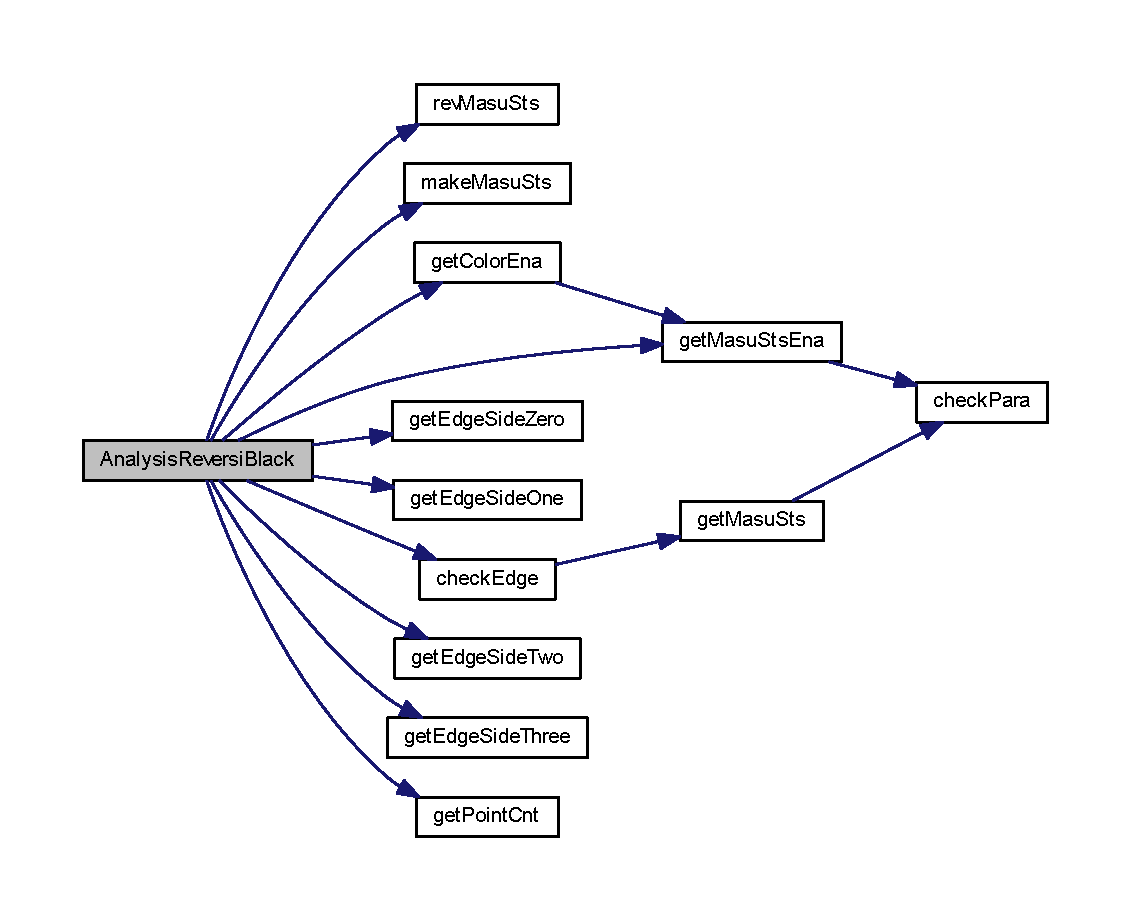
\includegraphics[width=350pt]{class_reversi_a471972ec549188f7eb701d57e14ae7a1_cgraph}
\end{center}
\end{figure}
Here is the caller graph for this function\+:\nopagebreak
\begin{figure}[H]
\begin{center}
\leavevmode
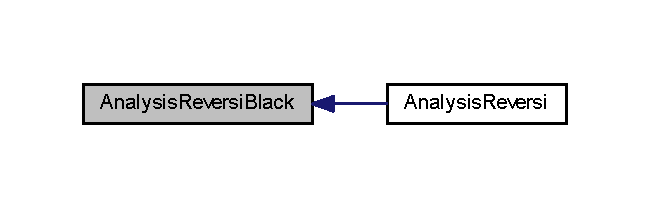
\includegraphics[width=312pt]{class_reversi_a471972ec549188f7eb701d57e14ae7a1_icgraph}
\end{center}
\end{figure}
\mbox{\Hypertarget{class_reversi_a3b581c4861bda72706a1d7146c910ad2}\label{class_reversi_a3b581c4861bda72706a1d7146c910ad2}} 
\index{Reversi@{Reversi}!Analysis\+Reversi\+Blue@{Analysis\+Reversi\+Blue}}
\index{Analysis\+Reversi\+Blue@{Analysis\+Reversi\+Blue}!Reversi@{Reversi}}
\subsubsection{\texorpdfstring{Analysis\+Reversi\+Blue()}{AnalysisReversiBlue()}}
{\footnotesize\ttfamily Analysis\+Reversi\+Blue (\begin{DoxyParamCaption}{ }\end{DoxyParamCaption})\hspace{0.3cm}{\ttfamily [private]}}



解析を行う(青) 

\begin{DoxyReturn}{Returns}
ありません 
\end{DoxyReturn}
\begin{DoxyAuthor}{Author}
Yuta Yoshinaga 
\end{DoxyAuthor}
\begin{DoxyDate}{Date}
2018.\+03.\+02 
\end{DoxyDate}


Definition at line 1112 of file Reversi.\+php.



Referenced by Analysis\+Reversi().

Here is the call graph for this function\+:\nopagebreak
\begin{figure}[H]
\begin{center}
\leavevmode
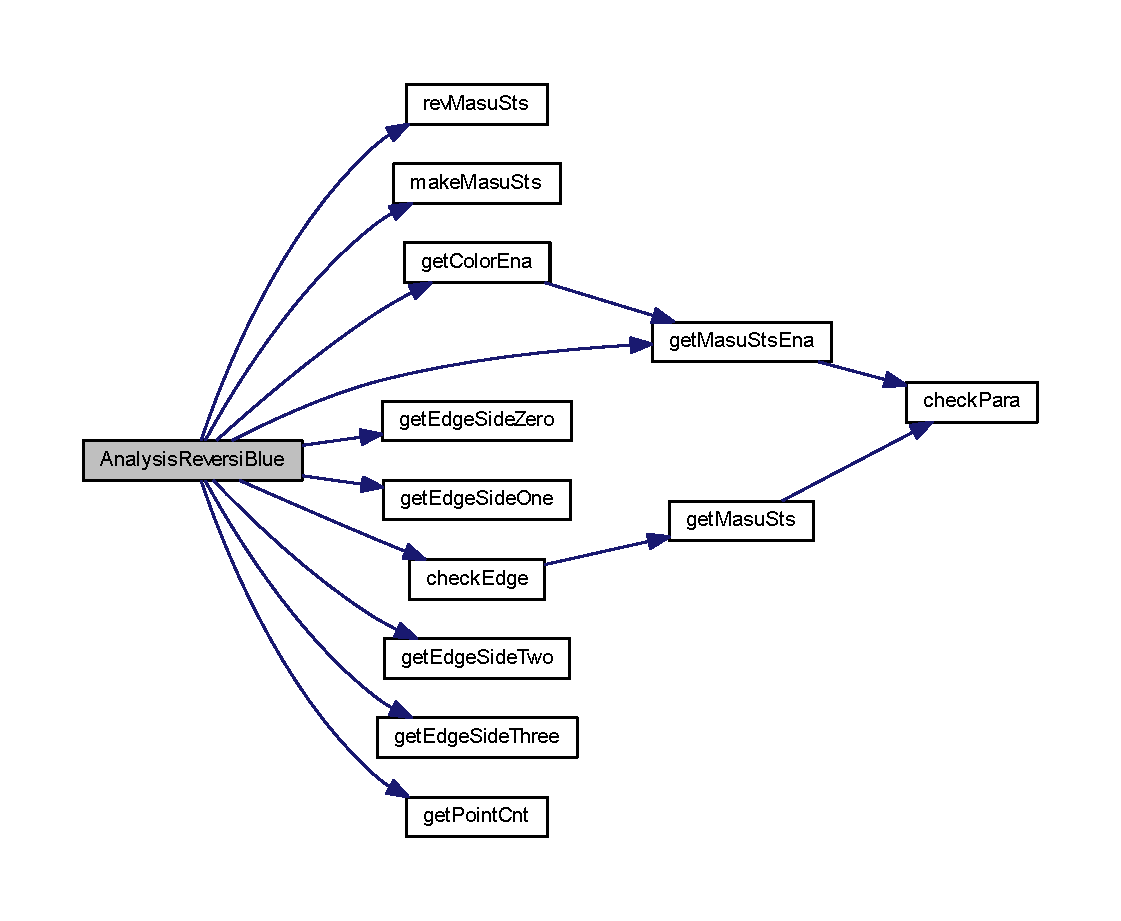
\includegraphics[width=350pt]{class_reversi_a3b581c4861bda72706a1d7146c910ad2_cgraph}
\end{center}
\end{figure}
Here is the caller graph for this function\+:\nopagebreak
\begin{figure}[H]
\begin{center}
\leavevmode
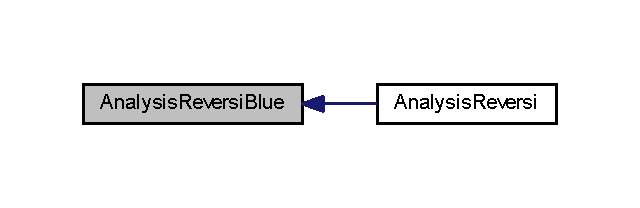
\includegraphics[width=307pt]{class_reversi_a3b581c4861bda72706a1d7146c910ad2_icgraph}
\end{center}
\end{figure}
\mbox{\Hypertarget{class_reversi_ad44cfa7c45a98365df2d6db094d61901}\label{class_reversi_ad44cfa7c45a98365df2d6db094d61901}} 
\index{Reversi@{Reversi}!Analysis\+Reversi\+Red@{Analysis\+Reversi\+Red}}
\index{Analysis\+Reversi\+Red@{Analysis\+Reversi\+Red}!Reversi@{Reversi}}
\subsubsection{\texorpdfstring{Analysis\+Reversi\+Red()}{AnalysisReversiRed()}}
{\footnotesize\ttfamily Analysis\+Reversi\+Red (\begin{DoxyParamCaption}{ }\end{DoxyParamCaption})\hspace{0.3cm}{\ttfamily [private]}}



解析を行う(赤) 

\begin{DoxyReturn}{Returns}
ありません 
\end{DoxyReturn}
\begin{DoxyAuthor}{Author}
Yuta Yoshinaga 
\end{DoxyAuthor}
\begin{DoxyDate}{Date}
2018.\+03.\+02 
\end{DoxyDate}


Definition at line 1269 of file Reversi.\+php.



Referenced by Analysis\+Reversi().

Here is the call graph for this function\+:\nopagebreak
\begin{figure}[H]
\begin{center}
\leavevmode
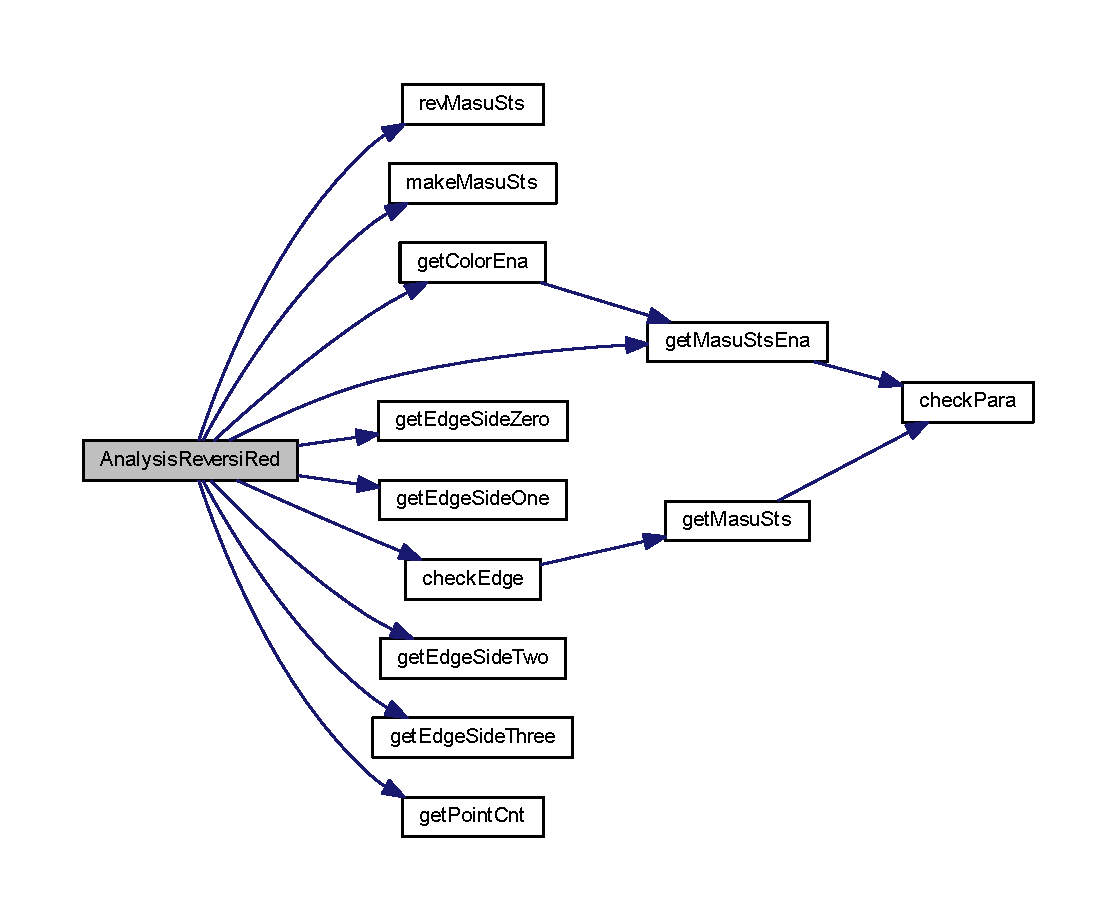
\includegraphics[width=350pt]{class_reversi_ad44cfa7c45a98365df2d6db094d61901_cgraph}
\end{center}
\end{figure}
Here is the caller graph for this function\+:\nopagebreak
\begin{figure}[H]
\begin{center}
\leavevmode
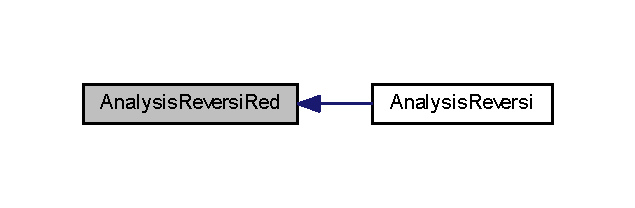
\includegraphics[width=305pt]{class_reversi_ad44cfa7c45a98365df2d6db094d61901_icgraph}
\end{center}
\end{figure}
\mbox{\Hypertarget{class_reversi_a3c30afb2509b0782b1c22a8770c68c48}\label{class_reversi_a3c30afb2509b0782b1c22a8770c68c48}} 
\index{Reversi@{Reversi}!Analysis\+Reversi\+White@{Analysis\+Reversi\+White}}
\index{Analysis\+Reversi\+White@{Analysis\+Reversi\+White}!Reversi@{Reversi}}
\subsubsection{\texorpdfstring{Analysis\+Reversi\+White()}{AnalysisReversiWhite()}}
{\footnotesize\ttfamily Analysis\+Reversi\+White (\begin{DoxyParamCaption}{ }\end{DoxyParamCaption})\hspace{0.3cm}{\ttfamily [private]}}



解析を行う(白) 

\begin{DoxyReturn}{Returns}
ありません 
\end{DoxyReturn}
\begin{DoxyAuthor}{Author}
Yuta Yoshinaga 
\end{DoxyAuthor}
\begin{DoxyDate}{Date}
2018.\+03.\+02 
\end{DoxyDate}


Definition at line 955 of file Reversi.\+php.



Referenced by Analysis\+Reversi().

Here is the call graph for this function\+:\nopagebreak
\begin{figure}[H]
\begin{center}
\leavevmode
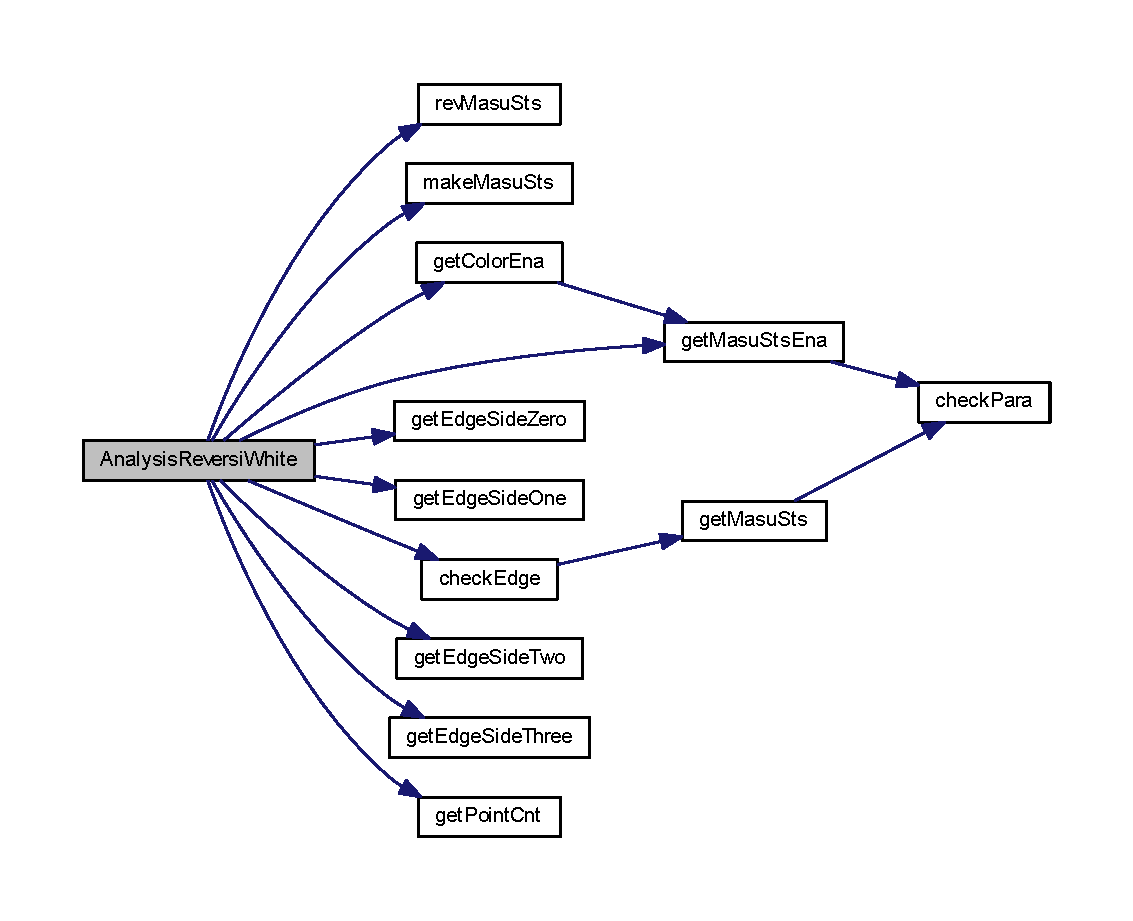
\includegraphics[width=350pt]{class_reversi_a3c30afb2509b0782b1c22a8770c68c48_cgraph}
\end{center}
\end{figure}
Here is the caller graph for this function\+:\nopagebreak
\begin{figure}[H]
\begin{center}
\leavevmode
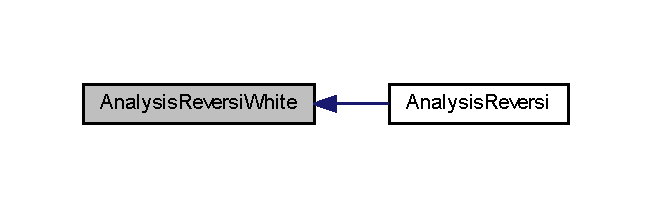
\includegraphics[width=313pt]{class_reversi_a3c30afb2509b0782b1c22a8770c68c48_icgraph}
\end{center}
\end{figure}
\mbox{\Hypertarget{class_reversi_acd2c64ea43cc26407ad64920a183446b}\label{class_reversi_acd2c64ea43cc26407ad64920a183446b}} 
\index{Reversi@{Reversi}!check\+Edge@{check\+Edge}}
\index{check\+Edge@{check\+Edge}!Reversi@{Reversi}}
\subsubsection{\texorpdfstring{check\+Edge()}{checkEdge()}}
{\footnotesize\ttfamily check\+Edge (\begin{DoxyParamCaption}\item[{}]{\$color,  }\item[{}]{\$y,  }\item[{}]{\$x }\end{DoxyParamCaption})}



角の隣に置いても角を取られないマス検索 


\begin{DoxyParams}[1]{Parameters}
\mbox{\tt in}  & {\em \$color} & コマ色 \\
\hline
\mbox{\tt in}  & {\em \$y} & マスの\$y座標 \\
\hline
\mbox{\tt in}  & {\em \$x} & マスの\$x座標 \\
\hline
\end{DoxyParams}
\begin{DoxyReturn}{Returns}
0 \+: 取られる それ以外 \+: 取られない 
\end{DoxyReturn}
\begin{DoxyAuthor}{Author}
Yuta Yoshinaga 
\end{DoxyAuthor}
\begin{DoxyDate}{Date}
2018.\+03.\+02 
\end{DoxyDate}


Definition at line 1825 of file Reversi.\+php.



Referenced by Analysis\+Reversi\+Black(), Analysis\+Reversi\+Blue(), Analysis\+Reversi\+Red(), and Analysis\+Reversi\+White().

Here is the call graph for this function\+:\nopagebreak
\begin{figure}[H]
\begin{center}
\leavevmode
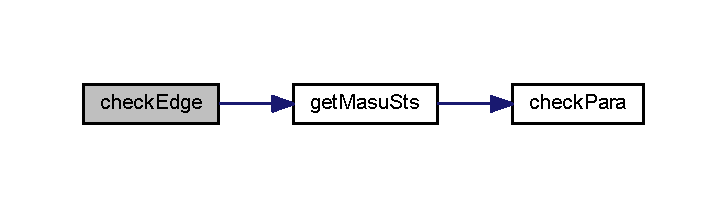
\includegraphics[width=349pt]{class_reversi_acd2c64ea43cc26407ad64920a183446b_cgraph}
\end{center}
\end{figure}
Here is the caller graph for this function\+:\nopagebreak
\begin{figure}[H]
\begin{center}
\leavevmode
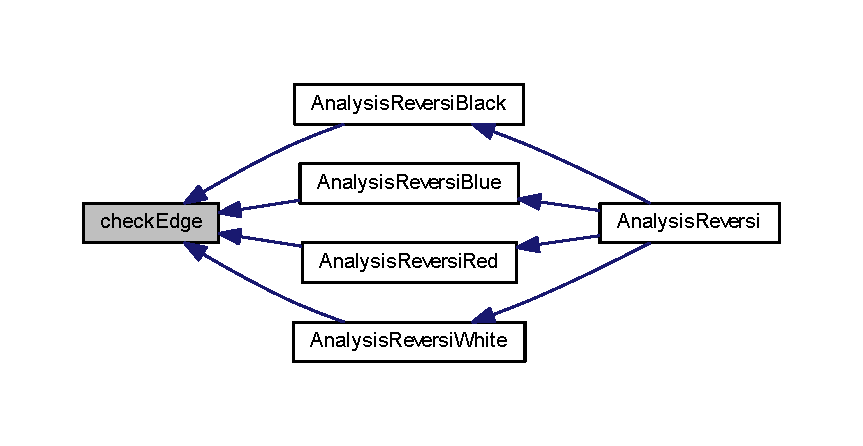
\includegraphics[width=350pt]{class_reversi_acd2c64ea43cc26407ad64920a183446b_icgraph}
\end{center}
\end{figure}
\mbox{\Hypertarget{class_reversi_ac8d57b64bc839c8bb1f53a2a5db11228}\label{class_reversi_ac8d57b64bc839c8bb1f53a2a5db11228}} 
\index{Reversi@{Reversi}!check\+Para@{check\+Para}}
\index{check\+Para@{check\+Para}!Reversi@{Reversi}}
\subsubsection{\texorpdfstring{check\+Para()}{checkPara()}}
{\footnotesize\ttfamily check\+Para (\begin{DoxyParamCaption}\item[{}]{\$para,  }\item[{}]{\$min,  }\item[{}]{\$max }\end{DoxyParamCaption})\hspace{0.3cm}{\ttfamily [private]}}



パラメーター範囲チェック 


\begin{DoxyParams}[1]{Parameters}
\mbox{\tt in}  & {\em \$para} & チェックパラメーター \\
\hline
\mbox{\tt in}  & {\em \$min} & パラメーター最小値 \\
\hline
\mbox{\tt in}  & {\em \$max} & パラメーター最大値 \\
\hline
\end{DoxyParams}
\begin{DoxyReturn}{Returns}
0 \+: 成功 それ以外 \+: 失敗 
\end{DoxyReturn}
\begin{DoxyAuthor}{Author}
Yuta Yoshinaga 
\end{DoxyAuthor}
\begin{DoxyDate}{Date}
2018.\+03.\+02 
\end{DoxyDate}


Definition at line 783 of file Reversi.\+php.



Referenced by get\+History(), get\+Masu\+Sts(), get\+Masu\+Sts\+Cnt(), get\+Masu\+Sts\+Ena(), get\+Masu\+Sts\+Old(), get\+Pass\+Ena(), get\+Point(), get\+Point\+Anz(), and set\+Masu\+Cnt().

Here is the caller graph for this function\+:\nopagebreak
\begin{figure}[H]
\begin{center}
\leavevmode
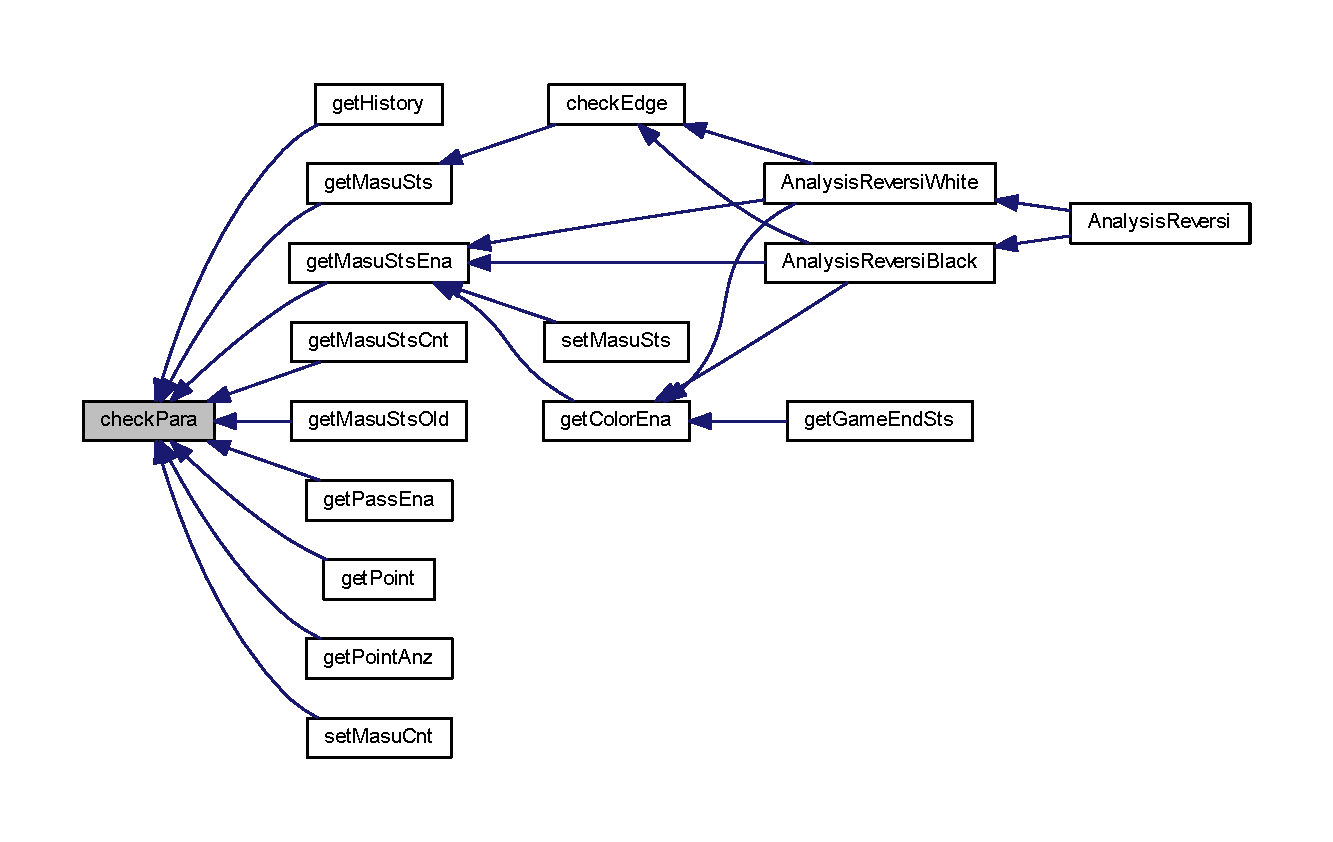
\includegraphics[width=350pt]{class_reversi_ac8d57b64bc839c8bb1f53a2a5db11228_icgraph}
\end{center}
\end{figure}
\mbox{\Hypertarget{class_reversi_acb1491c467c3065beece256256f5f59d}\label{class_reversi_acb1491c467c3065beece256256f5f59d}} 
\index{Reversi@{Reversi}!get\+Bet\+Cnt@{get\+Bet\+Cnt}}
\index{get\+Bet\+Cnt@{get\+Bet\+Cnt}!Reversi@{Reversi}}
\subsubsection{\texorpdfstring{get\+Bet\+Cnt()}{getBetCnt()}}
{\footnotesize\ttfamily get\+Bet\+Cnt (\begin{DoxyParamCaption}\item[{}]{\$color }\end{DoxyParamCaption})}



コマ数取得 


\begin{DoxyParams}[1]{Parameters}
\mbox{\tt in}  & {\em \$color} & コマ色 \\
\hline
\end{DoxyParams}
\begin{DoxyReturn}{Returns}
コマ数取得 
\end{DoxyReturn}
\begin{DoxyAuthor}{Author}
Yuta Yoshinaga 
\end{DoxyAuthor}
\begin{DoxyDate}{Date}
2018.\+03.\+02 
\end{DoxyDate}


Definition at line 1722 of file Reversi.\+php.

\mbox{\Hypertarget{class_reversi_aead5ee041feb6ac2609266614ea06f78}\label{class_reversi_aead5ee041feb6ac2609266614ea06f78}} 
\index{Reversi@{Reversi}!get\+Color\+Ena@{get\+Color\+Ena}}
\index{get\+Color\+Ena@{get\+Color\+Ena}!Reversi@{Reversi}}
\subsubsection{\texorpdfstring{get\+Color\+Ena()}{getColorEna()}}
{\footnotesize\ttfamily get\+Color\+Ena (\begin{DoxyParamCaption}\item[{}]{\$color }\end{DoxyParamCaption})}



指定色が現在置ける場所があるかチェック 


\begin{DoxyParams}[1]{Parameters}
\mbox{\tt in}  & {\em \$color} & コマ色 \\
\hline
\end{DoxyParams}
\begin{DoxyReturn}{Returns}
0 \+: 成功 それ以外 \+: 失敗 
\end{DoxyReturn}
\begin{DoxyAuthor}{Author}
Yuta Yoshinaga 
\end{DoxyAuthor}
\begin{DoxyDate}{Date}
2018.\+03.\+02 
\end{DoxyDate}


Definition at line 1563 of file Reversi.\+php.



Referenced by Analysis\+Reversi\+Black(), Analysis\+Reversi\+Blue(), Analysis\+Reversi\+Red(), Analysis\+Reversi\+White(), and get\+Game\+End\+Sts().

Here is the call graph for this function\+:\nopagebreak
\begin{figure}[H]
\begin{center}
\leavevmode
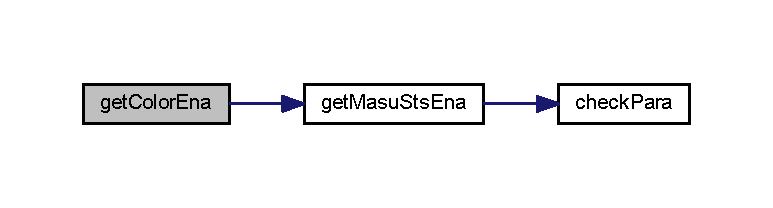
\includegraphics[width=350pt]{class_reversi_aead5ee041feb6ac2609266614ea06f78_cgraph}
\end{center}
\end{figure}
Here is the caller graph for this function\+:\nopagebreak
\begin{figure}[H]
\begin{center}
\leavevmode
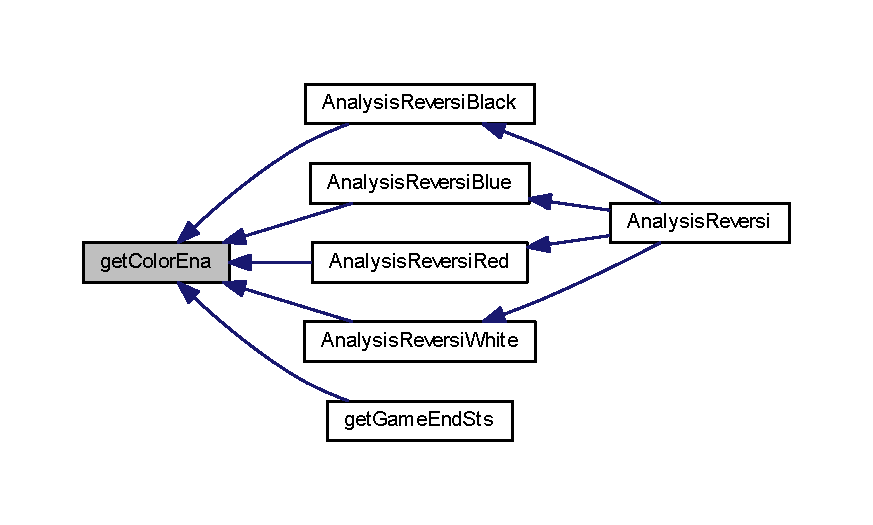
\includegraphics[width=350pt]{class_reversi_aead5ee041feb6ac2609266614ea06f78_icgraph}
\end{center}
\end{figure}
\mbox{\Hypertarget{class_reversi_a98aff7f2db3a9feacbe98293c6b80eb4}\label{class_reversi_a98aff7f2db3a9feacbe98293c6b80eb4}} 
\index{Reversi@{Reversi}!get\+Edge\+Side\+One@{get\+Edge\+Side\+One}}
\index{get\+Edge\+Side\+One@{get\+Edge\+Side\+One}!Reversi@{Reversi}}
\subsubsection{\texorpdfstring{get\+Edge\+Side\+One()}{getEdgeSideOne()}}
{\footnotesize\ttfamily get\+Edge\+Side\+One (\begin{DoxyParamCaption}\item[{}]{\$y,  }\item[{}]{\$x }\end{DoxyParamCaption})}



指定座標が角の一つ手前か取得 


\begin{DoxyParams}[1]{Parameters}
\mbox{\tt in}  & {\em \$y} & \$y座標 \\
\hline
\mbox{\tt in}  & {\em \$x} & \$x座標 \\
\hline
\end{DoxyParams}
\begin{DoxyReturn}{Returns}
0 \+: 成功 それ以外 \+: 失敗 
\end{DoxyReturn}
\begin{DoxyAuthor}{Author}
Yuta Yoshinaga 
\end{DoxyAuthor}
\begin{DoxyDate}{Date}
2018.\+03.\+02 
\end{DoxyDate}


Definition at line 1967 of file Reversi.\+php.



Referenced by Analysis\+Reversi\+Black(), Analysis\+Reversi\+Blue(), Analysis\+Reversi\+Red(), and Analysis\+Reversi\+White().

Here is the caller graph for this function\+:\nopagebreak
\begin{figure}[H]
\begin{center}
\leavevmode
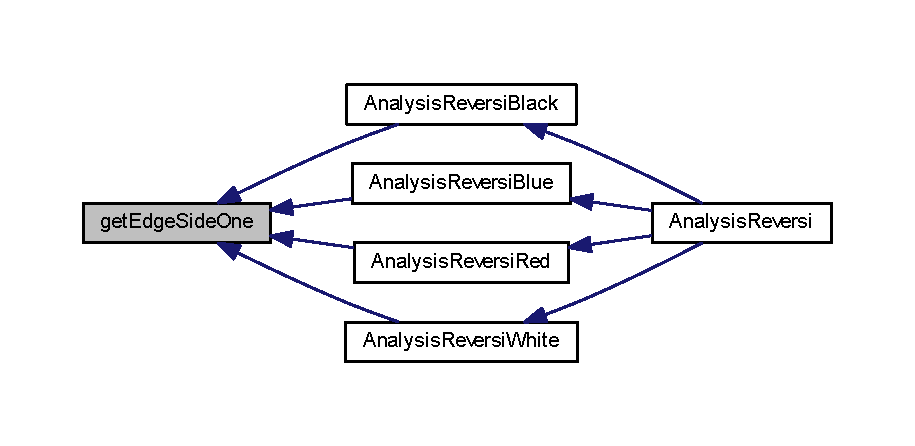
\includegraphics[width=350pt]{class_reversi_a98aff7f2db3a9feacbe98293c6b80eb4_icgraph}
\end{center}
\end{figure}
\mbox{\Hypertarget{class_reversi_ab299d2488c8ab29f646e449d3204efbc}\label{class_reversi_ab299d2488c8ab29f646e449d3204efbc}} 
\index{Reversi@{Reversi}!get\+Edge\+Side\+Three@{get\+Edge\+Side\+Three}}
\index{get\+Edge\+Side\+Three@{get\+Edge\+Side\+Three}!Reversi@{Reversi}}
\subsubsection{\texorpdfstring{get\+Edge\+Side\+Three()}{getEdgeSideThree()}}
{\footnotesize\ttfamily get\+Edge\+Side\+Three (\begin{DoxyParamCaption}\item[{}]{\$y,  }\item[{}]{\$x }\end{DoxyParamCaption})}



指定座標が角の三つ以上手前か取得 


\begin{DoxyParams}[1]{Parameters}
\mbox{\tt in}  & {\em \$y} & \$y座標 \\
\hline
\mbox{\tt in}  & {\em \$x} & \$x座標 \\
\hline
\end{DoxyParams}
\begin{DoxyReturn}{Returns}
0 \+: 成功 それ以外 \+: 失敗 
\end{DoxyReturn}
\begin{DoxyAuthor}{Author}
Yuta Yoshinaga 
\end{DoxyAuthor}
\begin{DoxyDate}{Date}
2018.\+03.\+02 
\end{DoxyDate}


Definition at line 2031 of file Reversi.\+php.



Referenced by Analysis\+Reversi\+Black(), Analysis\+Reversi\+Blue(), Analysis\+Reversi\+Red(), and Analysis\+Reversi\+White().

Here is the caller graph for this function\+:\nopagebreak
\begin{figure}[H]
\begin{center}
\leavevmode
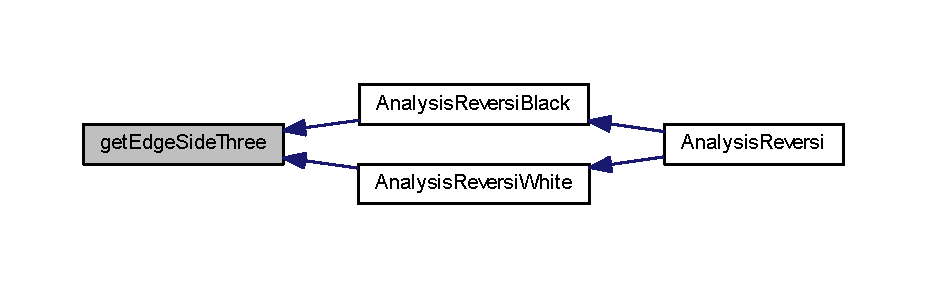
\includegraphics[width=350pt]{class_reversi_ab299d2488c8ab29f646e449d3204efbc_icgraph}
\end{center}
\end{figure}
\mbox{\Hypertarget{class_reversi_a968982683aa41f50c83789a9be05aaba}\label{class_reversi_a968982683aa41f50c83789a9be05aaba}} 
\index{Reversi@{Reversi}!get\+Edge\+Side\+Two@{get\+Edge\+Side\+Two}}
\index{get\+Edge\+Side\+Two@{get\+Edge\+Side\+Two}!Reversi@{Reversi}}
\subsubsection{\texorpdfstring{get\+Edge\+Side\+Two()}{getEdgeSideTwo()}}
{\footnotesize\ttfamily get\+Edge\+Side\+Two (\begin{DoxyParamCaption}\item[{}]{\$y,  }\item[{}]{\$x }\end{DoxyParamCaption})}



指定座標が角の二つ手前か取得 


\begin{DoxyParams}[1]{Parameters}
\mbox{\tt in}  & {\em \$y} & \$y座標 \\
\hline
\mbox{\tt in}  & {\em \$x} & \$x座標 \\
\hline
\end{DoxyParams}
\begin{DoxyReturn}{Returns}
0 \+: 成功 それ以外 \+: 失敗 
\end{DoxyReturn}
\begin{DoxyAuthor}{Author}
Yuta Yoshinaga 
\end{DoxyAuthor}
\begin{DoxyDate}{Date}
2018.\+03.\+02 
\end{DoxyDate}


Definition at line 1999 of file Reversi.\+php.



Referenced by Analysis\+Reversi\+Black(), Analysis\+Reversi\+Blue(), Analysis\+Reversi\+Red(), and Analysis\+Reversi\+White().

Here is the caller graph for this function\+:\nopagebreak
\begin{figure}[H]
\begin{center}
\leavevmode
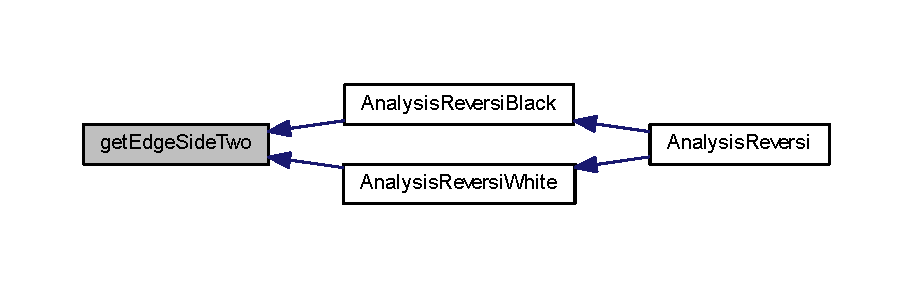
\includegraphics[width=350pt]{class_reversi_a968982683aa41f50c83789a9be05aaba_icgraph}
\end{center}
\end{figure}
\mbox{\Hypertarget{class_reversi_a76a7addedc2b0ba83c6b46ce0601076c}\label{class_reversi_a76a7addedc2b0ba83c6b46ce0601076c}} 
\index{Reversi@{Reversi}!get\+Edge\+Side\+Zero@{get\+Edge\+Side\+Zero}}
\index{get\+Edge\+Side\+Zero@{get\+Edge\+Side\+Zero}!Reversi@{Reversi}}
\subsubsection{\texorpdfstring{get\+Edge\+Side\+Zero()}{getEdgeSideZero()}}
{\footnotesize\ttfamily get\+Edge\+Side\+Zero (\begin{DoxyParamCaption}\item[{}]{\$y,  }\item[{}]{\$x }\end{DoxyParamCaption})}



指定座標が角か取得 


\begin{DoxyParams}[1]{Parameters}
\mbox{\tt in}  & {\em \$y} & \$y座標 \\
\hline
\mbox{\tt in}  & {\em \$x} & \$x座標 \\
\hline
\end{DoxyParams}
\begin{DoxyReturn}{Returns}
0 \+: 成功 それ以外 \+: 失敗 
\end{DoxyReturn}
\begin{DoxyAuthor}{Author}
Yuta Yoshinaga 
\end{DoxyAuthor}
\begin{DoxyDate}{Date}
2018.\+03.\+02 
\end{DoxyDate}


Definition at line 1943 of file Reversi.\+php.



Referenced by Analysis\+Reversi\+Black(), Analysis\+Reversi\+Blue(), Analysis\+Reversi\+Red(), and Analysis\+Reversi\+White().

Here is the caller graph for this function\+:\nopagebreak
\begin{figure}[H]
\begin{center}
\leavevmode
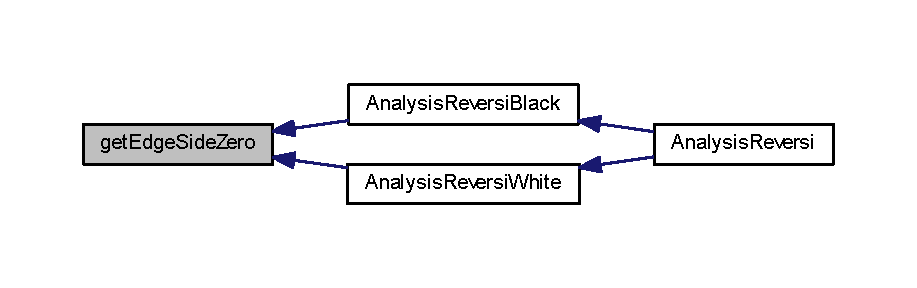
\includegraphics[width=350pt]{class_reversi_a76a7addedc2b0ba83c6b46ce0601076c_icgraph}
\end{center}
\end{figure}
\mbox{\Hypertarget{class_reversi_aab9985c789e464de6cf99d7d725cb5a3}\label{class_reversi_aab9985c789e464de6cf99d7d725cb5a3}} 
\index{Reversi@{Reversi}!get\+Game\+End\+Sts@{get\+Game\+End\+Sts}}
\index{get\+Game\+End\+Sts@{get\+Game\+End\+Sts}!Reversi@{Reversi}}
\subsubsection{\texorpdfstring{get\+Game\+End\+Sts()}{getGameEndSts()}}
{\footnotesize\ttfamily get\+Game\+End\+Sts (\begin{DoxyParamCaption}{ }\end{DoxyParamCaption})}



ゲーム終了かチェック 

\begin{DoxyReturn}{Returns}
0 \+: 続行 それ以外 \+: ゲーム終了 
\end{DoxyReturn}
\begin{DoxyAuthor}{Author}
Yuta Yoshinaga 
\end{DoxyAuthor}
\begin{DoxyDate}{Date}
2018.\+03.\+02 
\end{DoxyDate}


Definition at line 1585 of file Reversi.\+php.

Here is the call graph for this function\+:\nopagebreak
\begin{figure}[H]
\begin{center}
\leavevmode
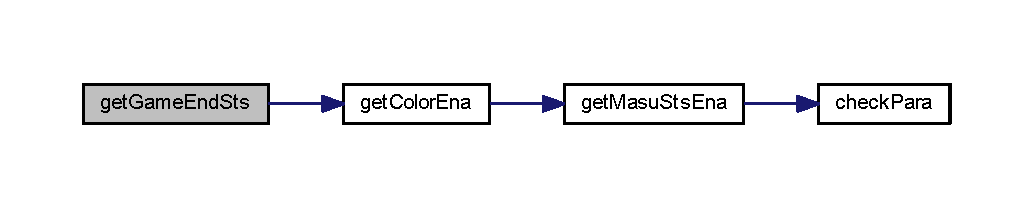
\includegraphics[width=350pt]{class_reversi_aab9985c789e464de6cf99d7d725cb5a3_cgraph}
\end{center}
\end{figure}
\mbox{\Hypertarget{class_reversi_a41cae82a798f2b3d0684bda44b837fcf}\label{class_reversi_a41cae82a798f2b3d0684bda44b837fcf}} 
\index{Reversi@{Reversi}!get\+History@{get\+History}}
\index{get\+History@{get\+History}!Reversi@{Reversi}}
\subsubsection{\texorpdfstring{get\+History()}{getHistory()}}
{\footnotesize\ttfamily get\+History (\begin{DoxyParamCaption}\item[{}]{\$num }\end{DoxyParamCaption})}



履歴取得 


\begin{DoxyParams}[1]{Parameters}
\mbox{\tt in}  & {\em \$num} & ポイント \\
\hline
\end{DoxyParams}
\begin{DoxyReturn}{Returns}
履歴 N\+U\+LL \+: 失敗 
\end{DoxyReturn}
\begin{DoxyAuthor}{Author}
Yuta Yoshinaga 
\end{DoxyAuthor}
\begin{DoxyDate}{Date}
2018.\+03.\+02 
\end{DoxyDate}


Definition at line 1767 of file Reversi.\+php.

Here is the call graph for this function\+:\nopagebreak
\begin{figure}[H]
\begin{center}
\leavevmode
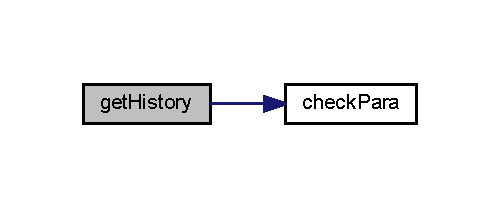
\includegraphics[width=240pt]{class_reversi_a41cae82a798f2b3d0684bda44b837fcf_cgraph}
\end{center}
\end{figure}
\mbox{\Hypertarget{class_reversi_a004834cf9f95ab56b62c1305bbc68ce2}\label{class_reversi_a004834cf9f95ab56b62c1305bbc68ce2}} 
\index{Reversi@{Reversi}!get\+History\+Cnt@{get\+History\+Cnt}}
\index{get\+History\+Cnt@{get\+History\+Cnt}!Reversi@{Reversi}}
\subsubsection{\texorpdfstring{get\+History\+Cnt()}{getHistoryCnt()}}
{\footnotesize\ttfamily get\+History\+Cnt (\begin{DoxyParamCaption}{ }\end{DoxyParamCaption})}



履歴数取得 

\begin{DoxyReturn}{Returns}
履歴数 
\end{DoxyReturn}
\begin{DoxyAuthor}{Author}
Yuta Yoshinaga 
\end{DoxyAuthor}
\begin{DoxyDate}{Date}
2018.\+03.\+02 
\end{DoxyDate}


Definition at line 1784 of file Reversi.\+php.

\mbox{\Hypertarget{class_reversi_a1baed538e7a503cd51850d368b9e65f7}\label{class_reversi_a1baed538e7a503cd51850d368b9e65f7}} 
\index{Reversi@{Reversi}!get\+Masu\+Sts@{get\+Masu\+Sts}}
\index{get\+Masu\+Sts@{get\+Masu\+Sts}!Reversi@{Reversi}}
\subsubsection{\texorpdfstring{get\+Masu\+Sts()}{getMasuSts()}}
{\footnotesize\ttfamily get\+Masu\+Sts (\begin{DoxyParamCaption}\item[{}]{\$y,  }\item[{}]{\$x }\end{DoxyParamCaption})}



マスステータスを取得 


\begin{DoxyParams}[1]{Parameters}
\mbox{\tt in}  & {\em \$y} & 取得するマスの\+Y座標 \\
\hline
\mbox{\tt in}  & {\em \$x} & 取得するマスの\+X座標 \\
\hline
\end{DoxyParams}
\begin{DoxyReturn}{Returns}
-\/1 \+: 失敗 それ以外 \+: マスステータス 
\end{DoxyReturn}
\begin{DoxyAuthor}{Author}
Yuta Yoshinaga 
\end{DoxyAuthor}
\begin{DoxyDate}{Date}
2018.\+03.\+02 
\end{DoxyDate}


Definition at line 1484 of file Reversi.\+php.



Referenced by check\+Edge().

Here is the call graph for this function\+:\nopagebreak
\begin{figure}[H]
\begin{center}
\leavevmode
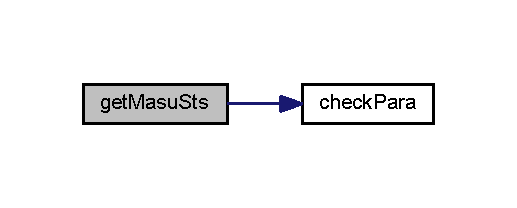
\includegraphics[width=248pt]{class_reversi_a1baed538e7a503cd51850d368b9e65f7_cgraph}
\end{center}
\end{figure}
Here is the caller graph for this function\+:\nopagebreak
\begin{figure}[H]
\begin{center}
\leavevmode
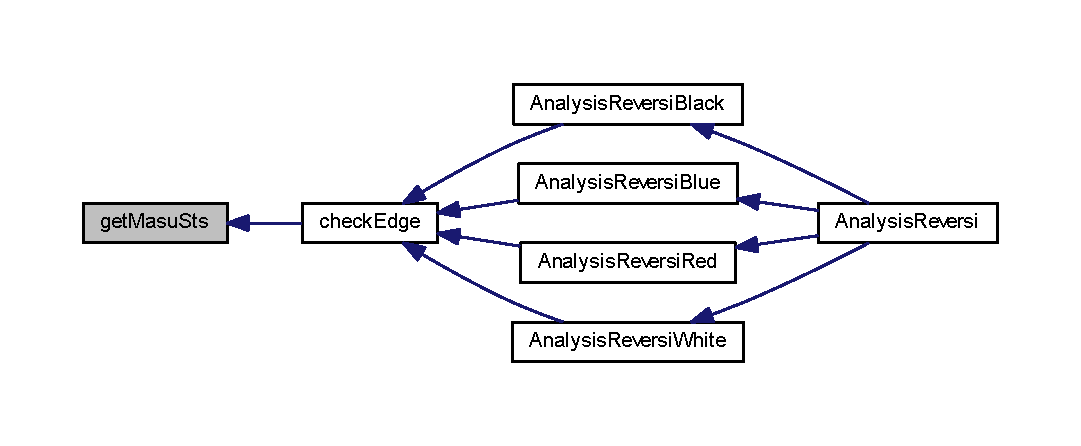
\includegraphics[width=350pt]{class_reversi_a1baed538e7a503cd51850d368b9e65f7_icgraph}
\end{center}
\end{figure}
\mbox{\Hypertarget{class_reversi_a10bfc13effc2db9a681a2906792be453}\label{class_reversi_a10bfc13effc2db9a681a2906792be453}} 
\index{Reversi@{Reversi}!get\+Masu\+Sts\+Cnt@{get\+Masu\+Sts\+Cnt}}
\index{get\+Masu\+Sts\+Cnt@{get\+Masu\+Sts\+Cnt}!Reversi@{Reversi}}
\subsubsection{\texorpdfstring{get\+Masu\+Sts\+Cnt()}{getMasuStsCnt()}}
{\footnotesize\ttfamily get\+Masu\+Sts\+Cnt (\begin{DoxyParamCaption}\item[{}]{\$color,  }\item[{}]{\$y,  }\item[{}]{\$x }\end{DoxyParamCaption})}



指定座標の獲得コマ数取得 


\begin{DoxyParams}[1]{Parameters}
\mbox{\tt in}  & {\em \$color} & コマ色 \\
\hline
\mbox{\tt in}  & {\em \$y} & マスの\$y座標 \\
\hline
\mbox{\tt in}  & {\em \$x} & マスの\$x座標 \\
\hline
\end{DoxyParams}
\begin{DoxyReturn}{Returns}
-\/1 \+: 失敗 それ以外 \+: 獲得コマ数 
\end{DoxyReturn}
\begin{DoxyAuthor}{Author}
Yuta Yoshinaga 
\end{DoxyAuthor}
\begin{DoxyDate}{Date}
2018.\+03.\+02 
\end{DoxyDate}


Definition at line 1542 of file Reversi.\+php.

Here is the call graph for this function\+:\nopagebreak
\begin{figure}[H]
\begin{center}
\leavevmode
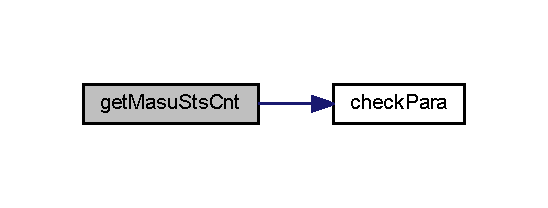
\includegraphics[width=263pt]{class_reversi_a10bfc13effc2db9a681a2906792be453_cgraph}
\end{center}
\end{figure}
\mbox{\Hypertarget{class_reversi_a22088e18c7f837f49093595261c30e4e}\label{class_reversi_a22088e18c7f837f49093595261c30e4e}} 
\index{Reversi@{Reversi}!get\+Masu\+Sts\+Ena@{get\+Masu\+Sts\+Ena}}
\index{get\+Masu\+Sts\+Ena@{get\+Masu\+Sts\+Ena}!Reversi@{Reversi}}
\subsubsection{\texorpdfstring{get\+Masu\+Sts\+Ena()}{getMasuStsEna()}}
{\footnotesize\ttfamily get\+Masu\+Sts\+Ena (\begin{DoxyParamCaption}\item[{}]{\$color,  }\item[{}]{\$y,  }\item[{}]{\$x }\end{DoxyParamCaption})}



指定座標に指定色を置けるかチェック 


\begin{DoxyParams}[1]{Parameters}
\mbox{\tt in}  & {\em \$color} & コマ色 \\
\hline
\mbox{\tt in}  & {\em \$y} & マスの\$y座標 \\
\hline
\mbox{\tt in}  & {\em \$x} & マスの\$x座標 \\
\hline
\end{DoxyParams}
\begin{DoxyReturn}{Returns}
1 \+: 成功 それ以外 \+: 失敗 
\end{DoxyReturn}
\begin{DoxyAuthor}{Author}
Yuta Yoshinaga 
\end{DoxyAuthor}
\begin{DoxyDate}{Date}
2018.\+03.\+02 
\end{DoxyDate}


Definition at line 1519 of file Reversi.\+php.



Referenced by Analysis\+Reversi\+Black(), Analysis\+Reversi\+Blue(), Analysis\+Reversi\+Red(), Analysis\+Reversi\+White(), get\+Color\+Ena(), and set\+Masu\+Sts().

Here is the call graph for this function\+:\nopagebreak
\begin{figure}[H]
\begin{center}
\leavevmode
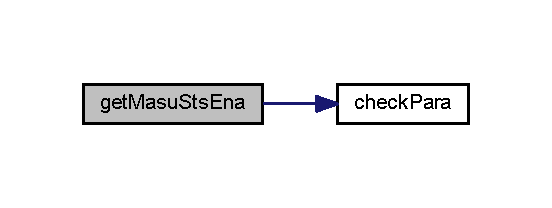
\includegraphics[width=265pt]{class_reversi_a22088e18c7f837f49093595261c30e4e_cgraph}
\end{center}
\end{figure}
Here is the caller graph for this function\+:\nopagebreak
\begin{figure}[H]
\begin{center}
\leavevmode
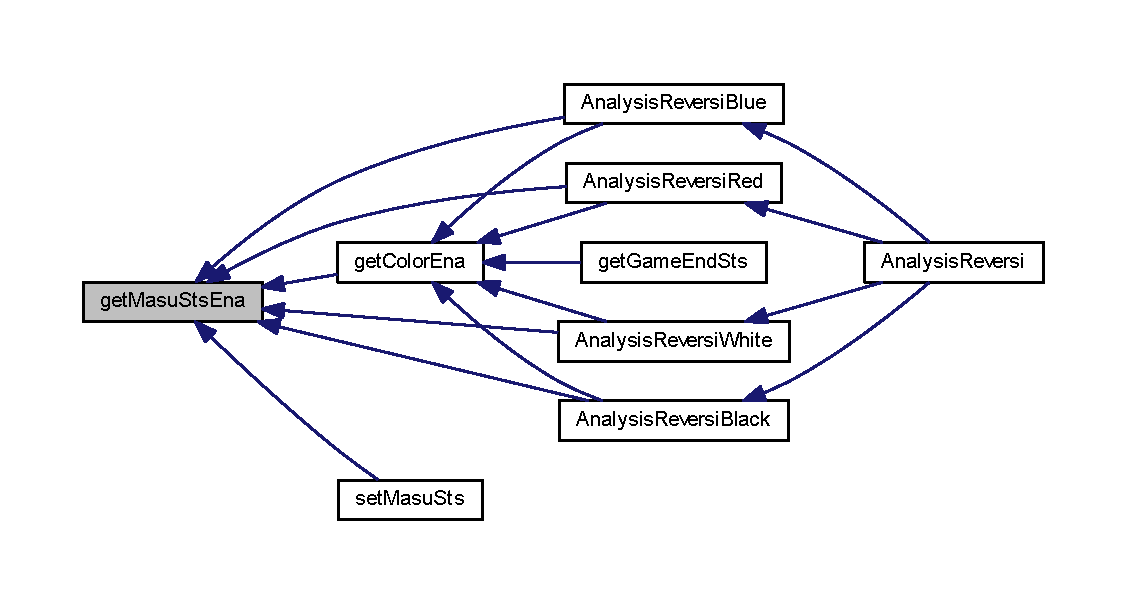
\includegraphics[width=350pt]{class_reversi_a22088e18c7f837f49093595261c30e4e_icgraph}
\end{center}
\end{figure}
\mbox{\Hypertarget{class_reversi_a1688a929d3917e19510f6501c42d6a2b}\label{class_reversi_a1688a929d3917e19510f6501c42d6a2b}} 
\index{Reversi@{Reversi}!get\+Masu\+Sts\+Old@{get\+Masu\+Sts\+Old}}
\index{get\+Masu\+Sts\+Old@{get\+Masu\+Sts\+Old}!Reversi@{Reversi}}
\subsubsection{\texorpdfstring{get\+Masu\+Sts\+Old()}{getMasuStsOld()}}
{\footnotesize\ttfamily get\+Masu\+Sts\+Old (\begin{DoxyParamCaption}\item[{}]{\$y,  }\item[{}]{\$x }\end{DoxyParamCaption})}



以前のマスステータスを取得 


\begin{DoxyParams}[1]{Parameters}
\mbox{\tt in}  & {\em y} & 取得するマスの\+Y座標 \\
\hline
\mbox{\tt in}  & {\em x} & 取得するマスの\+X座標 \\
\hline
\end{DoxyParams}
\begin{DoxyReturn}{Returns}
-\/1 \+: 失敗 それ以外 \+: マスステータス 
\end{DoxyReturn}
\begin{DoxyAuthor}{Author}
Yuta Yoshinaga 
\end{DoxyAuthor}
\begin{DoxyDate}{Date}
2018.\+03.\+02 
\end{DoxyDate}


Definition at line 1501 of file Reversi.\+php.

Here is the call graph for this function\+:\nopagebreak
\begin{figure}[H]
\begin{center}
\leavevmode
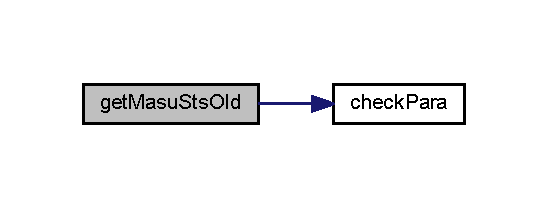
\includegraphics[width=263pt]{class_reversi_a1688a929d3917e19510f6501c42d6a2b_cgraph}
\end{center}
\end{figure}
\mbox{\Hypertarget{class_reversi_a123959981f8e1d48fc7b9d183a5c6d0a}\label{class_reversi_a123959981f8e1d48fc7b9d183a5c6d0a}} 
\index{Reversi@{Reversi}!get\+Pass\+Ena@{get\+Pass\+Ena}}
\index{get\+Pass\+Ena@{get\+Pass\+Ena}!Reversi@{Reversi}}
\subsubsection{\texorpdfstring{get\+Pass\+Ena()}{getPassEna()}}
{\footnotesize\ttfamily get\+Pass\+Ena (\begin{DoxyParamCaption}\item[{}]{\$color,  }\item[{}]{\$y,  }\item[{}]{\$x }\end{DoxyParamCaption})}



パス判定 


\begin{DoxyParams}[1]{Parameters}
\mbox{\tt in}  & {\em \$color} & コマ色 \\
\hline
\mbox{\tt in}  & {\em \$y} & マスの\+Y座標 \\
\hline
\mbox{\tt in}  & {\em \$x} & マスの\+X座標 \\
\hline
\end{DoxyParams}
\begin{DoxyReturn}{Returns}
パス判定
\begin{DoxyItemize}
\item 0 \+: N\+OT P\+A\+SS
\item 1 \+: P\+A\+SS
\end{DoxyItemize}
\end{DoxyReturn}
\begin{DoxyAuthor}{Author}
Yuta Yoshinaga 
\end{DoxyAuthor}
\begin{DoxyDate}{Date}
2018.\+03.\+02 
\end{DoxyDate}


Definition at line 1746 of file Reversi.\+php.

Here is the call graph for this function\+:\nopagebreak
\begin{figure}[H]
\begin{center}
\leavevmode
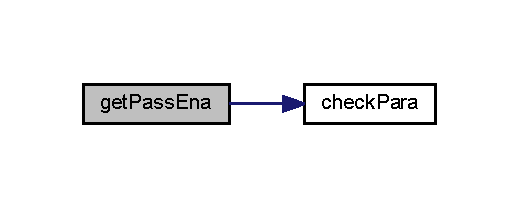
\includegraphics[width=249pt]{class_reversi_a123959981f8e1d48fc7b9d183a5c6d0a_cgraph}
\end{center}
\end{figure}
\mbox{\Hypertarget{class_reversi_ad059cc09b0001edd980f43770380b863}\label{class_reversi_ad059cc09b0001edd980f43770380b863}} 
\index{Reversi@{Reversi}!get\+Point@{get\+Point}}
\index{get\+Point@{get\+Point}!Reversi@{Reversi}}
\subsubsection{\texorpdfstring{get\+Point()}{getPoint()}}
{\footnotesize\ttfamily get\+Point (\begin{DoxyParamCaption}\item[{}]{\$color,  }\item[{}]{\$num }\end{DoxyParamCaption})}



ポイント座標取得 


\begin{DoxyParams}[1]{Parameters}
\mbox{\tt in}  & {\em \$color} & コマ色 \\
\hline
\mbox{\tt in}  & {\em \$num} & ポイント \\
\hline
\end{DoxyParams}
\begin{DoxyReturn}{Returns}
ポイント座標 N\+U\+LL \+: 失敗 
\end{DoxyReturn}
\begin{DoxyAuthor}{Author}
Yuta Yoshinaga 
\end{DoxyAuthor}
\begin{DoxyDate}{Date}
2018.\+03.\+02 
\end{DoxyDate}


Definition at line 1682 of file Reversi.\+php.

Here is the call graph for this function\+:\nopagebreak
\begin{figure}[H]
\begin{center}
\leavevmode
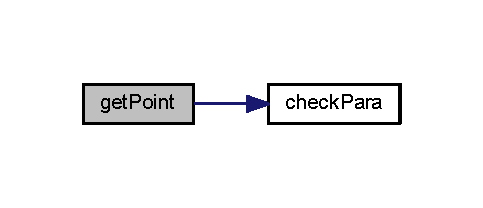
\includegraphics[width=232pt]{class_reversi_ad059cc09b0001edd980f43770380b863_cgraph}
\end{center}
\end{figure}
\mbox{\Hypertarget{class_reversi_af1a30d438a7d17f31353b9d4bfe9cb65}\label{class_reversi_af1a30d438a7d17f31353b9d4bfe9cb65}} 
\index{Reversi@{Reversi}!get\+Point\+Anz@{get\+Point\+Anz}}
\index{get\+Point\+Anz@{get\+Point\+Anz}!Reversi@{Reversi}}
\subsubsection{\texorpdfstring{get\+Point\+Anz()}{getPointAnz()}}
{\footnotesize\ttfamily get\+Point\+Anz (\begin{DoxyParamCaption}\item[{}]{\$color,  }\item[{}]{\$y,  }\item[{}]{\$x }\end{DoxyParamCaption})}



ポイント座標解析取得 


\begin{DoxyParams}[1]{Parameters}
\mbox{\tt in}  & {\em \$color} & コマ色 \\
\hline
\mbox{\tt in}  & {\em \$y} & マスの\$y座標 \\
\hline
\mbox{\tt in}  & {\em \$x} & マスの\$x座標 \\
\hline
\end{DoxyParams}
\begin{DoxyReturn}{Returns}
ポイント座標解析 N\+U\+LL \+: 失敗 
\end{DoxyReturn}
\begin{DoxyAuthor}{Author}
Yuta Yoshinaga 
\end{DoxyAuthor}
\begin{DoxyDate}{Date}
2018.\+03.\+02 
\end{DoxyDate}


Definition at line 1802 of file Reversi.\+php.

Here is the call graph for this function\+:\nopagebreak
\begin{figure}[H]
\begin{center}
\leavevmode
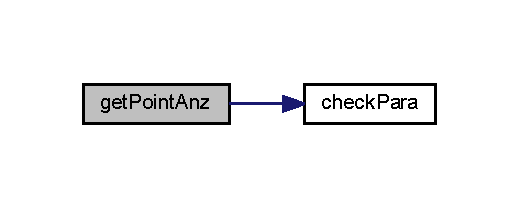
\includegraphics[width=249pt]{class_reversi_af1a30d438a7d17f31353b9d4bfe9cb65_cgraph}
\end{center}
\end{figure}
\mbox{\Hypertarget{class_reversi_af538d04718f177f71461f582f3bd8eba}\label{class_reversi_af538d04718f177f71461f582f3bd8eba}} 
\index{Reversi@{Reversi}!get\+Point\+Cnt@{get\+Point\+Cnt}}
\index{get\+Point\+Cnt@{get\+Point\+Cnt}!Reversi@{Reversi}}
\subsubsection{\texorpdfstring{get\+Point\+Cnt()}{getPointCnt()}}
{\footnotesize\ttfamily get\+Point\+Cnt (\begin{DoxyParamCaption}\item[{}]{\$color }\end{DoxyParamCaption})}



ポイント座標数取得 


\begin{DoxyParams}[1]{Parameters}
\mbox{\tt in}  & {\em \$color} & コマ色 \\
\hline
\end{DoxyParams}
\begin{DoxyReturn}{Returns}
ポイント座標数取得 
\end{DoxyReturn}
\begin{DoxyAuthor}{Author}
Yuta Yoshinaga 
\end{DoxyAuthor}
\begin{DoxyDate}{Date}
2018.\+03.\+02 
\end{DoxyDate}


Definition at line 1703 of file Reversi.\+php.



Referenced by Analysis\+Reversi\+Black(), Analysis\+Reversi\+Blue(), Analysis\+Reversi\+Red(), and Analysis\+Reversi\+White().

Here is the caller graph for this function\+:\nopagebreak
\begin{figure}[H]
\begin{center}
\leavevmode
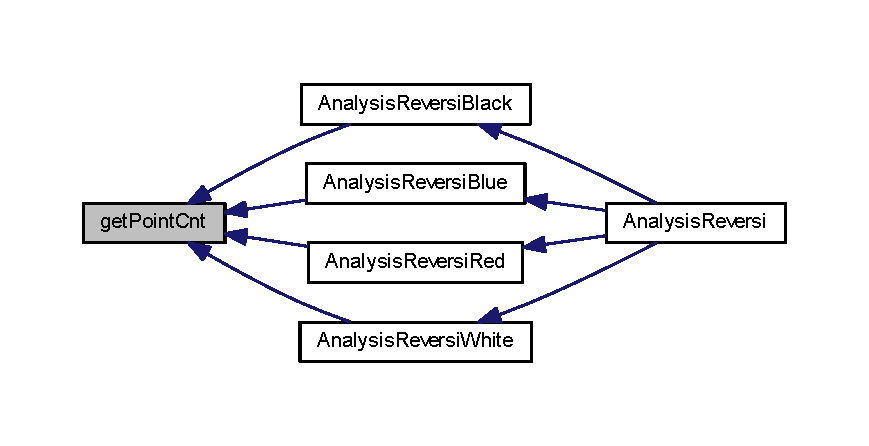
\includegraphics[width=350pt]{class_reversi_af538d04718f177f71461f582f3bd8eba_icgraph}
\end{center}
\end{figure}
\mbox{\Hypertarget{class_reversi_a88869682786bb7c45c3488113deaa789}\label{class_reversi_a88869682786bb7c45c3488113deaa789}} 
\index{Reversi@{Reversi}!make\+Masu\+Sts@{make\+Masu\+Sts}}
\index{make\+Masu\+Sts@{make\+Masu\+Sts}!Reversi@{Reversi}}
\subsubsection{\texorpdfstring{make\+Masu\+Sts()}{makeMasuSts()}}
{\footnotesize\ttfamily make\+Masu\+Sts (\begin{DoxyParamCaption}\item[{}]{\$color }\end{DoxyParamCaption})\hspace{0.3cm}{\ttfamily [private]}}



各コマの置ける場所等のステータス作成 


\begin{DoxyParams}[1]{Parameters}
\mbox{\tt in}  & {\em \$color} & ステータスを作成するコマ \\
\hline
\end{DoxyParams}
\begin{DoxyReturn}{Returns}
ありません 
\end{DoxyReturn}
\begin{DoxyAuthor}{Author}
Yuta Yoshinaga 
\end{DoxyAuthor}
\begin{DoxyDate}{Date}
2018.\+03.\+02 
\end{DoxyDate}


Definition at line 357 of file Reversi.\+php.



Referenced by Analysis\+Reversi(), Analysis\+Reversi\+Black(), Analysis\+Reversi\+Blue(), Analysis\+Reversi\+Red(), Analysis\+Reversi\+White(), reset(), and set\+Masu\+Sts().

Here is the caller graph for this function\+:\nopagebreak
\begin{figure}[H]
\begin{center}
\leavevmode
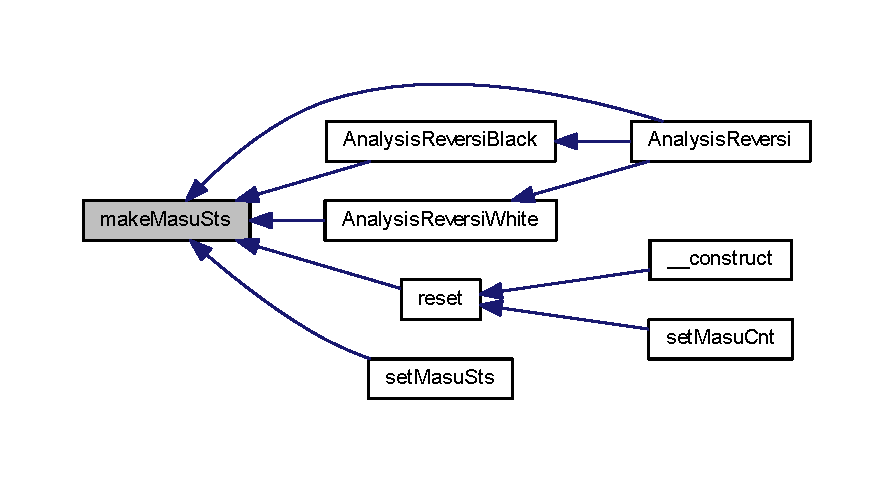
\includegraphics[width=350pt]{class_reversi_a88869682786bb7c45c3488113deaa789_icgraph}
\end{center}
\end{figure}
\mbox{\Hypertarget{class_reversi_a4a20559544fdf4dcb457e258dc976cf8}\label{class_reversi_a4a20559544fdf4dcb457e258dc976cf8}} 
\index{Reversi@{Reversi}!reset@{reset}}
\index{reset@{reset}!Reversi@{Reversi}}
\subsubsection{\texorpdfstring{reset()}{reset()}}
{\footnotesize\ttfamily reset (\begin{DoxyParamCaption}{ }\end{DoxyParamCaption})}



リセット 

\begin{DoxyReturn}{Returns}
ありません 
\end{DoxyReturn}
\begin{DoxyAuthor}{Author}
Yuta Yoshinaga 
\end{DoxyAuthor}
\begin{DoxyDate}{Date}
2018.\+03.\+02 
\end{DoxyDate}


Definition at line 306 of file Reversi.\+php.



Referenced by \+\_\+\+\_\+construct(), and set\+Masu\+Cnt().

Here is the call graph for this function\+:\nopagebreak
\begin{figure}[H]
\begin{center}
\leavevmode
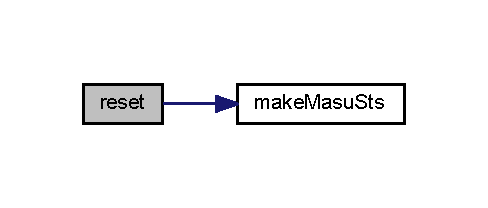
\includegraphics[width=234pt]{class_reversi_a4a20559544fdf4dcb457e258dc976cf8_cgraph}
\end{center}
\end{figure}
Here is the caller graph for this function\+:\nopagebreak
\begin{figure}[H]
\begin{center}
\leavevmode
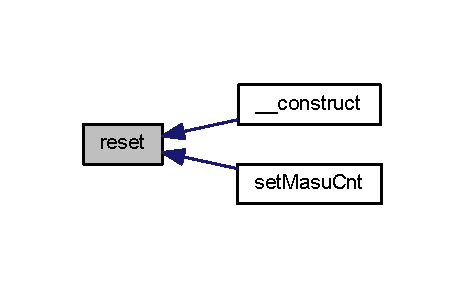
\includegraphics[width=223pt]{class_reversi_a4a20559544fdf4dcb457e258dc976cf8_icgraph}
\end{center}
\end{figure}
\mbox{\Hypertarget{class_reversi_af29cd3f41dc1cffead056dbbed55ae7a}\label{class_reversi_af29cd3f41dc1cffead056dbbed55ae7a}} 
\index{Reversi@{Reversi}!rev\+Masu\+Sts@{rev\+Masu\+Sts}}
\index{rev\+Masu\+Sts@{rev\+Masu\+Sts}!Reversi@{Reversi}}
\subsubsection{\texorpdfstring{rev\+Masu\+Sts()}{revMasuSts()}}
{\footnotesize\ttfamily rev\+Masu\+Sts (\begin{DoxyParamCaption}\item[{}]{\$color,  }\item[{}]{\$y,  }\item[{}]{\$x }\end{DoxyParamCaption})\hspace{0.3cm}{\ttfamily [private]}}



コマをひっくり返す 


\begin{DoxyParams}[1]{Parameters}
\mbox{\tt in}  & {\em \$color} & ひっくり返す元コマ \\
\hline
\mbox{\tt in}  & {\em \$y} & ひっくり返す元コマの\$y座標 \\
\hline
\mbox{\tt in}  & {\em \$x} & ひっくり返す元コマの\$x座標 \\
\hline
\end{DoxyParams}
\begin{DoxyReturn}{Returns}
ありません 
\end{DoxyReturn}
\begin{DoxyAuthor}{Author}
Yuta Yoshinaga 
\end{DoxyAuthor}
\begin{DoxyDate}{Date}
2018.\+03.\+02 
\end{DoxyDate}


Definition at line 607 of file Reversi.\+php.



Referenced by Analysis\+Reversi\+Black(), Analysis\+Reversi\+Blue(), Analysis\+Reversi\+Red(), Analysis\+Reversi\+White(), and set\+Masu\+Sts().

Here is the caller graph for this function\+:\nopagebreak
\begin{figure}[H]
\begin{center}
\leavevmode
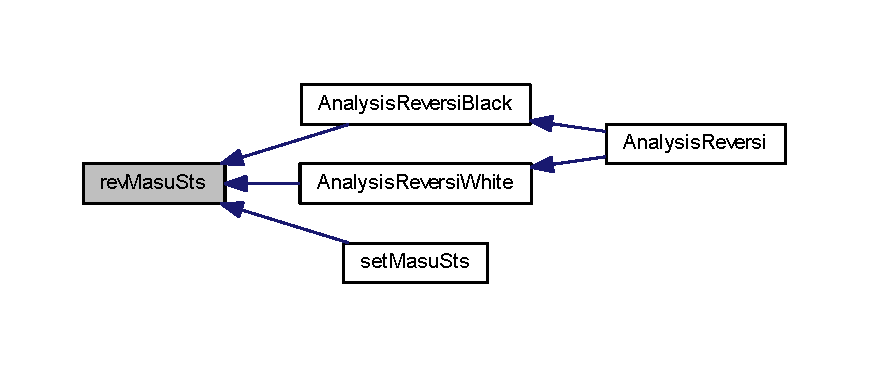
\includegraphics[width=350pt]{class_reversi_af29cd3f41dc1cffead056dbbed55ae7a_icgraph}
\end{center}
\end{figure}
\mbox{\Hypertarget{class_reversi_ab6853cc0f53e50a70d576f15296f0864}\label{class_reversi_ab6853cc0f53e50a70d576f15296f0864}} 
\index{Reversi@{Reversi}!set\+Masu\+Cnt@{set\+Masu\+Cnt}}
\index{set\+Masu\+Cnt@{set\+Masu\+Cnt}!Reversi@{Reversi}}
\subsubsection{\texorpdfstring{set\+Masu\+Cnt()}{setMasuCnt()}}
{\footnotesize\ttfamily set\+Masu\+Cnt (\begin{DoxyParamCaption}\item[{}]{\$cnt }\end{DoxyParamCaption})}



マスの数変更 


\begin{DoxyParams}[1]{Parameters}
\mbox{\tt in}  & {\em \$cnt} & マスの数 \\
\hline
\end{DoxyParams}
\begin{DoxyReturn}{Returns}
0 \+: 成功 それ以外 \+: 失敗 
\end{DoxyReturn}
\begin{DoxyAuthor}{Author}
Yuta Yoshinaga 
\end{DoxyAuthor}
\begin{DoxyDate}{Date}
2018.\+03.\+02 
\end{DoxyDate}


Definition at line 1657 of file Reversi.\+php.

Here is the call graph for this function\+:\nopagebreak
\begin{figure}[H]
\begin{center}
\leavevmode
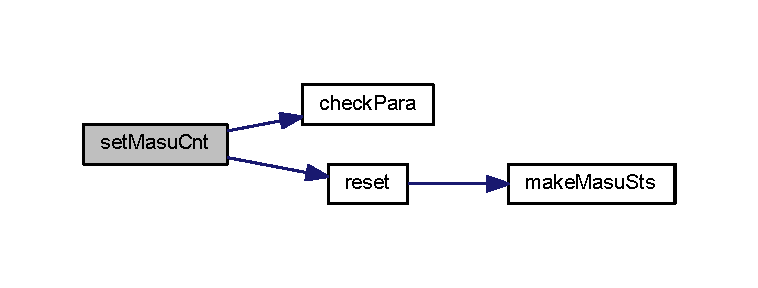
\includegraphics[width=350pt]{class_reversi_ab6853cc0f53e50a70d576f15296f0864_cgraph}
\end{center}
\end{figure}
\mbox{\Hypertarget{class_reversi_a26f3168c7d94e70d344841d65885a4ac}\label{class_reversi_a26f3168c7d94e70d344841d65885a4ac}} 
\index{Reversi@{Reversi}!set\+Masu\+Sts@{set\+Masu\+Sts}}
\index{set\+Masu\+Sts@{set\+Masu\+Sts}!Reversi@{Reversi}}
\subsubsection{\texorpdfstring{set\+Masu\+Sts()}{setMasuSts()}}
{\footnotesize\ttfamily set\+Masu\+Sts (\begin{DoxyParamCaption}\item[{}]{\$color,  }\item[{}]{\$y,  }\item[{}]{\$x }\end{DoxyParamCaption})}



指定座標にコマを置く 


\begin{DoxyParams}[1]{Parameters}
\mbox{\tt in}  & {\em \$color} & コマ色 \\
\hline
\mbox{\tt in}  & {\em \$y} & マスの\$y座標 \\
\hline
\mbox{\tt in}  & {\em \$x} & マスの\$x座標 \\
\hline
\end{DoxyParams}
\begin{DoxyReturn}{Returns}
0 \+: 成功 それ以外 \+: 失敗 
\end{DoxyReturn}
\begin{DoxyAuthor}{Author}
Yuta Yoshinaga 
\end{DoxyAuthor}
\begin{DoxyDate}{Date}
2018.\+03.\+02 
\end{DoxyDate}


Definition at line 1606 of file Reversi.\+php.

Here is the call graph for this function\+:\nopagebreak
\begin{figure}[H]
\begin{center}
\leavevmode
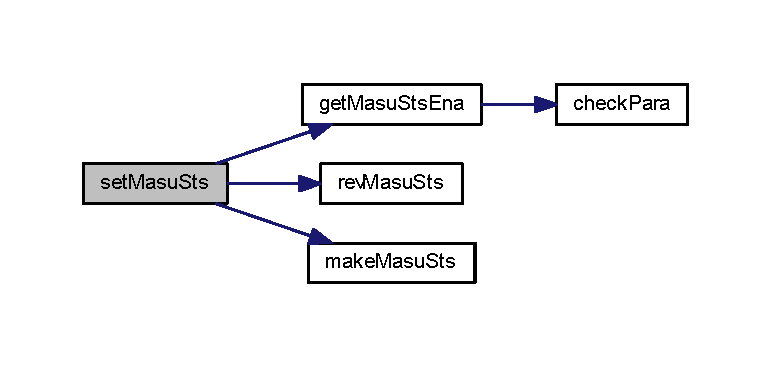
\includegraphics[width=350pt]{class_reversi_a26f3168c7d94e70d344841d65885a4ac_cgraph}
\end{center}
\end{figure}
\mbox{\Hypertarget{class_reversi_ae659a2ce33e395f8d5cda5e62d03fe7e}\label{class_reversi_ae659a2ce33e395f8d5cda5e62d03fe7e}} 
\index{Reversi@{Reversi}!set\+Masu\+Sts\+Forcibly@{set\+Masu\+Sts\+Forcibly}}
\index{set\+Masu\+Sts\+Forcibly@{set\+Masu\+Sts\+Forcibly}!Reversi@{Reversi}}
\subsubsection{\texorpdfstring{set\+Masu\+Sts\+Forcibly()}{setMasuStsForcibly()}}
{\footnotesize\ttfamily set\+Masu\+Sts\+Forcibly (\begin{DoxyParamCaption}\item[{}]{\$color,  }\item[{}]{\$y,  }\item[{}]{\$x }\end{DoxyParamCaption})}



指定座標にコマを強制的に置く 


\begin{DoxyParams}[1]{Parameters}
\mbox{\tt in}  & {\em \$color} & コマ色 \\
\hline
\mbox{\tt in}  & {\em \$y} & マスの\$y座標 \\
\hline
\mbox{\tt in}  & {\em \$x} & マスの\$x座標 \\
\hline
\end{DoxyParams}
\begin{DoxyReturn}{Returns}
0 \+: 成功 それ以外 \+: 失敗 
\end{DoxyReturn}
\begin{DoxyAuthor}{Author}
Yuta Yoshinaga 
\end{DoxyAuthor}
\begin{DoxyDate}{Date}
2018.\+03.\+02 
\end{DoxyDate}


Definition at line 1640 of file Reversi.\+php.



The documentation for this class was generated from the following file\+:\begin{DoxyCompactItemize}
\item 
Model/\hyperlink{_reversi_8php}{Reversi.\+php}\end{DoxyCompactItemize}

\hypertarget{class_reversi_anz}{}\section{Reversi\+Anz Class Reference}
\label{class_reversi_anz}\index{Reversi\+Anz@{Reversi\+Anz}}


リバーシ解析クラス  




Collaboration diagram for Reversi\+Anz\+:
\nopagebreak
\begin{figure}[H]
\begin{center}
\leavevmode
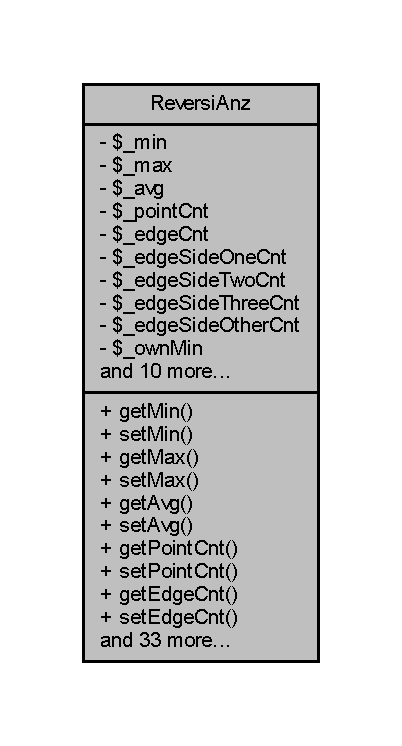
\includegraphics[width=193pt]{class_reversi_anz__coll__graph}
\end{center}
\end{figure}
\subsection*{Public Member Functions}
\begin{DoxyCompactItemize}
\item 
\mbox{\Hypertarget{class_reversi_anz_a8404d3eedbf6483ec27f13f64f9df3b1}\label{class_reversi_anz_a8404d3eedbf6483ec27f13f64f9df3b1}} 
{\bfseries get\+Min} ()
\item 
\mbox{\Hypertarget{class_reversi_anz_a6567c1122f96ec079b2f64f887e3543f}\label{class_reversi_anz_a6567c1122f96ec079b2f64f887e3543f}} 
{\bfseries set\+Min} (\$\+\_\+min)
\item 
\mbox{\Hypertarget{class_reversi_anz_abeb2912350107c52d5320b68beaceae7}\label{class_reversi_anz_abeb2912350107c52d5320b68beaceae7}} 
{\bfseries get\+Max} ()
\item 
\mbox{\Hypertarget{class_reversi_anz_a31a31b0d815ac3f3e26a67310269282a}\label{class_reversi_anz_a31a31b0d815ac3f3e26a67310269282a}} 
{\bfseries set\+Max} (\$\+\_\+max)
\item 
\mbox{\Hypertarget{class_reversi_anz_a62d13c383b8902de0b1f1f76d4b3b4d9}\label{class_reversi_anz_a62d13c383b8902de0b1f1f76d4b3b4d9}} 
{\bfseries get\+Avg} ()
\item 
\mbox{\Hypertarget{class_reversi_anz_a430a846117accd844d205cb8bbc4b1f1}\label{class_reversi_anz_a430a846117accd844d205cb8bbc4b1f1}} 
{\bfseries set\+Avg} (\$\+\_\+avg)
\item 
\mbox{\Hypertarget{class_reversi_anz_a86da928704556cffeb9eb19b1020beff}\label{class_reversi_anz_a86da928704556cffeb9eb19b1020beff}} 
{\bfseries get\+Point\+Cnt} ()
\item 
\mbox{\Hypertarget{class_reversi_anz_aa9f4140eed7e8d282ddf617def3c3c70}\label{class_reversi_anz_aa9f4140eed7e8d282ddf617def3c3c70}} 
{\bfseries set\+Point\+Cnt} (\$\+\_\+point\+Cnt)
\item 
\mbox{\Hypertarget{class_reversi_anz_ac54bb2c81080ef8d6ae1ce1cf0f108bd}\label{class_reversi_anz_ac54bb2c81080ef8d6ae1ce1cf0f108bd}} 
{\bfseries get\+Edge\+Cnt} ()
\item 
\mbox{\Hypertarget{class_reversi_anz_a83947131d9c16ac8d0368234fbc273d7}\label{class_reversi_anz_a83947131d9c16ac8d0368234fbc273d7}} 
{\bfseries set\+Edge\+Cnt} (\$\+\_\+edge\+Cnt)
\item 
\mbox{\Hypertarget{class_reversi_anz_a1376e55e83fd05a9e29ca173425967f8}\label{class_reversi_anz_a1376e55e83fd05a9e29ca173425967f8}} 
{\bfseries get\+Edge\+Side\+One\+Cnt} ()
\item 
\mbox{\Hypertarget{class_reversi_anz_ad127ab3ba9b82be673950d183347c85e}\label{class_reversi_anz_ad127ab3ba9b82be673950d183347c85e}} 
{\bfseries set\+Edge\+Side\+One\+Cnt} (\$\+\_\+edge\+Side\+One\+Cnt)
\item 
\mbox{\Hypertarget{class_reversi_anz_a94d3fa39f3752df50f020a778e0c48a4}\label{class_reversi_anz_a94d3fa39f3752df50f020a778e0c48a4}} 
{\bfseries get\+Edge\+Side\+Two\+Cnt} ()
\item 
\mbox{\Hypertarget{class_reversi_anz_a4746c6d3580ede0a67a4d254a7f62bee}\label{class_reversi_anz_a4746c6d3580ede0a67a4d254a7f62bee}} 
{\bfseries set\+Edge\+Side\+Two\+Cnt} (\$\+\_\+edge\+Side\+Two\+Cnt)
\item 
\mbox{\Hypertarget{class_reversi_anz_ae26a95d517a16d416be4126522fb532f}\label{class_reversi_anz_ae26a95d517a16d416be4126522fb532f}} 
{\bfseries get\+Edge\+Side\+Three\+Cnt} ()
\item 
\mbox{\Hypertarget{class_reversi_anz_ac42ae43a9931dd7765f5650cf2881f3f}\label{class_reversi_anz_ac42ae43a9931dd7765f5650cf2881f3f}} 
{\bfseries set\+Edge\+Side\+Three\+Cnt} (\$\+\_\+edge\+Side\+Three\+Cnt)
\item 
\mbox{\Hypertarget{class_reversi_anz_a7b064999c75b33d3dafd636885a30660}\label{class_reversi_anz_a7b064999c75b33d3dafd636885a30660}} 
{\bfseries get\+Edge\+Side\+Other\+Cnt} ()
\item 
\mbox{\Hypertarget{class_reversi_anz_ad7d598abd2e505884b4e405505c81cdf}\label{class_reversi_anz_ad7d598abd2e505884b4e405505c81cdf}} 
{\bfseries set\+Edge\+Side\+Other\+Cnt} (\$\+\_\+edge\+Side\+Other\+Cnt)
\item 
\mbox{\Hypertarget{class_reversi_anz_a52453994039cc16cd883b615580bd678}\label{class_reversi_anz_a52453994039cc16cd883b615580bd678}} 
{\bfseries get\+Own\+Min} ()
\item 
\mbox{\Hypertarget{class_reversi_anz_aba52773abcdb9adc2b222977153c6a91}\label{class_reversi_anz_aba52773abcdb9adc2b222977153c6a91}} 
{\bfseries set\+Own\+Min} (\$\+\_\+own\+Min)
\item 
\mbox{\Hypertarget{class_reversi_anz_ae8b22c114dd706252d7ac65db730c4bd}\label{class_reversi_anz_ae8b22c114dd706252d7ac65db730c4bd}} 
{\bfseries get\+Own\+Max} ()
\item 
\mbox{\Hypertarget{class_reversi_anz_a0e115c41bc381831f3f1e19c3214eba7}\label{class_reversi_anz_a0e115c41bc381831f3f1e19c3214eba7}} 
{\bfseries set\+Own\+Max} (\$\+\_\+own\+Max)
\item 
\mbox{\Hypertarget{class_reversi_anz_a7dc0022c2e3015837f9443887fa970a1}\label{class_reversi_anz_a7dc0022c2e3015837f9443887fa970a1}} 
{\bfseries get\+Own\+Avg} ()
\item 
\mbox{\Hypertarget{class_reversi_anz_a7afbb115589b1cd369caf987326b5b83}\label{class_reversi_anz_a7afbb115589b1cd369caf987326b5b83}} 
{\bfseries set\+Own\+Avg} (\$\+\_\+own\+Avg)
\item 
\mbox{\Hypertarget{class_reversi_anz_aef6ff585777c6778cb8148833fc41451}\label{class_reversi_anz_aef6ff585777c6778cb8148833fc41451}} 
{\bfseries get\+Own\+Point\+Cnt} ()
\item 
\mbox{\Hypertarget{class_reversi_anz_a1f532e6595b9012475d07f90715fa35f}\label{class_reversi_anz_a1f532e6595b9012475d07f90715fa35f}} 
{\bfseries set\+Own\+Point\+Cnt} (\$\+\_\+own\+Point\+Cnt)
\item 
\mbox{\Hypertarget{class_reversi_anz_af630ff89845fd014edd5c53b6fb9f59d}\label{class_reversi_anz_af630ff89845fd014edd5c53b6fb9f59d}} 
{\bfseries get\+Own\+Edge\+Cnt} ()
\item 
\mbox{\Hypertarget{class_reversi_anz_adb980dd708ea8224fd02212b56d3ce30}\label{class_reversi_anz_adb980dd708ea8224fd02212b56d3ce30}} 
{\bfseries set\+Own\+Edge\+Cnt} (\$\+\_\+own\+Edge\+Cnt)
\item 
\mbox{\Hypertarget{class_reversi_anz_a04420643dba77a4d180877f38a7b20bb}\label{class_reversi_anz_a04420643dba77a4d180877f38a7b20bb}} 
{\bfseries get\+Own\+Edge\+Side\+One\+Cnt} ()
\item 
\mbox{\Hypertarget{class_reversi_anz_af3fbb8b287e10b57b5d926f78f94f096}\label{class_reversi_anz_af3fbb8b287e10b57b5d926f78f94f096}} 
{\bfseries set\+Own\+Edge\+Side\+One\+Cnt} (\$\+\_\+own\+Edge\+Side\+One\+Cnt)
\item 
\mbox{\Hypertarget{class_reversi_anz_aff7eba60fd808062aaa6079750000acc}\label{class_reversi_anz_aff7eba60fd808062aaa6079750000acc}} 
{\bfseries get\+Own\+Edge\+Side\+Two\+Cnt} ()
\item 
\mbox{\Hypertarget{class_reversi_anz_afddabe459e1b4482aadc432141ba6fe5}\label{class_reversi_anz_afddabe459e1b4482aadc432141ba6fe5}} 
{\bfseries set\+Own\+Edge\+Side\+Two\+Cnt} (\$\+\_\+own\+Edge\+Side\+Two\+Cnt)
\item 
\mbox{\Hypertarget{class_reversi_anz_addeed894b9ab975b3d6a1ad28a1467ad}\label{class_reversi_anz_addeed894b9ab975b3d6a1ad28a1467ad}} 
{\bfseries get\+Own\+Edge\+Side\+Three\+Cnt} ()
\item 
\mbox{\Hypertarget{class_reversi_anz_a04b6cf91352234e65db3b482b5dafcd8}\label{class_reversi_anz_a04b6cf91352234e65db3b482b5dafcd8}} 
{\bfseries set\+Own\+Edge\+Side\+Three\+Cnt} (\$\+\_\+own\+Edge\+Side\+Three\+Cnt)
\item 
\mbox{\Hypertarget{class_reversi_anz_a2d0001fd4c483bced75b8e581cc00acf}\label{class_reversi_anz_a2d0001fd4c483bced75b8e581cc00acf}} 
{\bfseries get\+Own\+Edge\+Side\+Other\+Cnt} ()
\item 
\mbox{\Hypertarget{class_reversi_anz_ac76d5718ad81e097eb9c273b183a1262}\label{class_reversi_anz_ac76d5718ad81e097eb9c273b183a1262}} 
{\bfseries set\+Own\+Edge\+Side\+Other\+Cnt} (\$\+\_\+own\+Edge\+Side\+Other\+Cnt)
\item 
\mbox{\Hypertarget{class_reversi_anz_ab2a185790727e92d925cb3baf69c3d82}\label{class_reversi_anz_ab2a185790727e92d925cb3baf69c3d82}} 
{\bfseries get\+Bad\+Point} ()
\item 
\mbox{\Hypertarget{class_reversi_anz_a2907c9b2a0659904b5d36900797ec5c0}\label{class_reversi_anz_a2907c9b2a0659904b5d36900797ec5c0}} 
{\bfseries set\+Bad\+Point} (\$\+\_\+bad\+Point)
\item 
\mbox{\Hypertarget{class_reversi_anz_a43bc56b57caeb7e1db0066f93e62abd6}\label{class_reversi_anz_a43bc56b57caeb7e1db0066f93e62abd6}} 
{\bfseries get\+Good\+Point} ()
\item 
\mbox{\Hypertarget{class_reversi_anz_acbbbe1567d8e903078b73049b40aa689}\label{class_reversi_anz_acbbbe1567d8e903078b73049b40aa689}} 
{\bfseries set\+Good\+Point} (\$\+\_\+good\+Point)
\item 
\hyperlink{class_reversi_anz_a095c5d389db211932136b53f25f39685}{\+\_\+\+\_\+construct} ()
\begin{DoxyCompactList}\small\item\em コンストラクタ \end{DoxyCompactList}\item 
\hyperlink{class_reversi_anz_a421831a265621325e1fdd19aace0c758}{\+\_\+\+\_\+destruct} ()
\begin{DoxyCompactList}\small\item\em デストラクタ \end{DoxyCompactList}\item 
\hyperlink{class_reversi_anz_a4a20559544fdf4dcb457e258dc976cf8}{reset} ()
\begin{DoxyCompactList}\small\item\em リセット \end{DoxyCompactList}\end{DoxyCompactItemize}
\subsection*{Private Attributes}
\begin{DoxyCompactItemize}
\item 
\mbox{\Hypertarget{class_reversi_anz_ae268ad2868ae3e63e753d709ea83ff8c}\label{class_reversi_anz_ae268ad2868ae3e63e753d709ea83ff8c}} 
\hyperlink{class_reversi_anz_ae268ad2868ae3e63e753d709ea83ff8c}{\$\+\_\+min}
\begin{DoxyCompactList}\small\item\em 最小値 \end{DoxyCompactList}\item 
\mbox{\Hypertarget{class_reversi_anz_a03d7199ef0a0f57557579b2c68c903fd}\label{class_reversi_anz_a03d7199ef0a0f57557579b2c68c903fd}} 
\hyperlink{class_reversi_anz_a03d7199ef0a0f57557579b2c68c903fd}{\$\+\_\+max}
\begin{DoxyCompactList}\small\item\em 最大値 \end{DoxyCompactList}\item 
\mbox{\Hypertarget{class_reversi_anz_a7010adfa47d0c21665753ac9010fc86e}\label{class_reversi_anz_a7010adfa47d0c21665753ac9010fc86e}} 
\hyperlink{class_reversi_anz_a7010adfa47d0c21665753ac9010fc86e}{\$\+\_\+avg}
\begin{DoxyCompactList}\small\item\em 平均 \end{DoxyCompactList}\item 
\mbox{\Hypertarget{class_reversi_anz_ac8c1f97213414e2aae74ab734086eba1}\label{class_reversi_anz_ac8c1f97213414e2aae74ab734086eba1}} 
\hyperlink{class_reversi_anz_ac8c1f97213414e2aae74ab734086eba1}{\$\+\_\+point\+Cnt}
\begin{DoxyCompactList}\small\item\em 置けるポイント数 \end{DoxyCompactList}\item 
\mbox{\Hypertarget{class_reversi_anz_a276ec7259be48b6cfd5c3211661c71fe}\label{class_reversi_anz_a276ec7259be48b6cfd5c3211661c71fe}} 
\hyperlink{class_reversi_anz_a276ec7259be48b6cfd5c3211661c71fe}{\$\+\_\+edge\+Cnt}
\begin{DoxyCompactList}\small\item\em 角を取れるポイント数 \end{DoxyCompactList}\item 
\mbox{\Hypertarget{class_reversi_anz_a471d69c419fa3fa86ee418063de71a55}\label{class_reversi_anz_a471d69c419fa3fa86ee418063de71a55}} 
\hyperlink{class_reversi_anz_a471d69c419fa3fa86ee418063de71a55}{\$\+\_\+edge\+Side\+One\+Cnt}
\begin{DoxyCompactList}\small\item\em 角一つ前を取れるポイント数 \end{DoxyCompactList}\item 
\mbox{\Hypertarget{class_reversi_anz_ab5ad0d1298fea7d4252b3d44adbd0065}\label{class_reversi_anz_ab5ad0d1298fea7d4252b3d44adbd0065}} 
\hyperlink{class_reversi_anz_ab5ad0d1298fea7d4252b3d44adbd0065}{\$\+\_\+edge\+Side\+Two\+Cnt}
\begin{DoxyCompactList}\small\item\em 角二つ前を取れるポイント数 \end{DoxyCompactList}\item 
\mbox{\Hypertarget{class_reversi_anz_a551631ced796e20f1601cc7222b4d609}\label{class_reversi_anz_a551631ced796e20f1601cc7222b4d609}} 
\hyperlink{class_reversi_anz_a551631ced796e20f1601cc7222b4d609}{\$\+\_\+edge\+Side\+Three\+Cnt}
\begin{DoxyCompactList}\small\item\em 角三つ前を取れるポイント数 \end{DoxyCompactList}\item 
\mbox{\Hypertarget{class_reversi_anz_a9c8a2f65aea73e6d823dba13279e347d}\label{class_reversi_anz_a9c8a2f65aea73e6d823dba13279e347d}} 
\hyperlink{class_reversi_anz_a9c8a2f65aea73e6d823dba13279e347d}{\$\+\_\+edge\+Side\+Other\+Cnt}
\begin{DoxyCompactList}\small\item\em それ以外を取れるポイント数 \end{DoxyCompactList}\item 
\mbox{\Hypertarget{class_reversi_anz_a23507611dd78fe72f00f5257a1462a90}\label{class_reversi_anz_a23507611dd78fe72f00f5257a1462a90}} 
\hyperlink{class_reversi_anz_a23507611dd78fe72f00f5257a1462a90}{\$\+\_\+own\+Min}
\begin{DoxyCompactList}\small\item\em 最小値 \end{DoxyCompactList}\item 
\mbox{\Hypertarget{class_reversi_anz_a397f5440a9b7b62b95be57bfbf7217ea}\label{class_reversi_anz_a397f5440a9b7b62b95be57bfbf7217ea}} 
\hyperlink{class_reversi_anz_a397f5440a9b7b62b95be57bfbf7217ea}{\$\+\_\+own\+Max}
\begin{DoxyCompactList}\small\item\em 最大値 \end{DoxyCompactList}\item 
\mbox{\Hypertarget{class_reversi_anz_a1fd406cb6004275a184a1c6bd082633c}\label{class_reversi_anz_a1fd406cb6004275a184a1c6bd082633c}} 
\hyperlink{class_reversi_anz_a1fd406cb6004275a184a1c6bd082633c}{\$\+\_\+own\+Avg}
\begin{DoxyCompactList}\small\item\em 平均 \end{DoxyCompactList}\item 
\mbox{\Hypertarget{class_reversi_anz_a36659c8ac9da31a82e205027bd318ff0}\label{class_reversi_anz_a36659c8ac9da31a82e205027bd318ff0}} 
\hyperlink{class_reversi_anz_a36659c8ac9da31a82e205027bd318ff0}{\$\+\_\+own\+Point\+Cnt}
\begin{DoxyCompactList}\small\item\em 置けるポイント数 \end{DoxyCompactList}\item 
\mbox{\Hypertarget{class_reversi_anz_a6473fea57c9615683452d10a560676ae}\label{class_reversi_anz_a6473fea57c9615683452d10a560676ae}} 
\hyperlink{class_reversi_anz_a6473fea57c9615683452d10a560676ae}{\$\+\_\+own\+Edge\+Cnt}
\begin{DoxyCompactList}\small\item\em 角を取れるポイント数 \end{DoxyCompactList}\item 
\mbox{\Hypertarget{class_reversi_anz_a0a15641c5318f85a658381c52a89ea7c}\label{class_reversi_anz_a0a15641c5318f85a658381c52a89ea7c}} 
\hyperlink{class_reversi_anz_a0a15641c5318f85a658381c52a89ea7c}{\$\+\_\+own\+Edge\+Side\+One\+Cnt}
\begin{DoxyCompactList}\small\item\em 角一つ前を取れるポイント数 \end{DoxyCompactList}\item 
\mbox{\Hypertarget{class_reversi_anz_a4b5e2654a0e2ef3654a899009f9730b9}\label{class_reversi_anz_a4b5e2654a0e2ef3654a899009f9730b9}} 
\hyperlink{class_reversi_anz_a4b5e2654a0e2ef3654a899009f9730b9}{\$\+\_\+own\+Edge\+Side\+Two\+Cnt}
\begin{DoxyCompactList}\small\item\em 角二つ前を取れるポイント数 \end{DoxyCompactList}\item 
\mbox{\Hypertarget{class_reversi_anz_a8b205636061577ffcdd595d2dfcc25d6}\label{class_reversi_anz_a8b205636061577ffcdd595d2dfcc25d6}} 
\hyperlink{class_reversi_anz_a8b205636061577ffcdd595d2dfcc25d6}{\$\+\_\+own\+Edge\+Side\+Three\+Cnt}
\begin{DoxyCompactList}\small\item\em 角三つ前を取れるポイント数 \end{DoxyCompactList}\item 
\mbox{\Hypertarget{class_reversi_anz_ac1532291c809b3924ea2f4fafddfdc8c}\label{class_reversi_anz_ac1532291c809b3924ea2f4fafddfdc8c}} 
\hyperlink{class_reversi_anz_ac1532291c809b3924ea2f4fafddfdc8c}{\$\+\_\+own\+Edge\+Side\+Other\+Cnt}
\begin{DoxyCompactList}\small\item\em それ以外を取れるポイント数 \end{DoxyCompactList}\item 
\mbox{\Hypertarget{class_reversi_anz_a325823c6f74529902667f01e8cfb62ca}\label{class_reversi_anz_a325823c6f74529902667f01e8cfb62ca}} 
\hyperlink{class_reversi_anz_a325823c6f74529902667f01e8cfb62ca}{\$\+\_\+bad\+Point}
\begin{DoxyCompactList}\small\item\em 悪手ポイント \end{DoxyCompactList}\item 
\mbox{\Hypertarget{class_reversi_anz_a311c8f84b5ca7f222d3c84c1e6251191}\label{class_reversi_anz_a311c8f84b5ca7f222d3c84c1e6251191}} 
\hyperlink{class_reversi_anz_a311c8f84b5ca7f222d3c84c1e6251191}{\$\+\_\+good\+Point}
\begin{DoxyCompactList}\small\item\em 良手ポイント \end{DoxyCompactList}\end{DoxyCompactItemize}


\subsection{Detailed Description}
リバーシ解析クラス 

Definition at line 25 of file Reversi\+Anz.\+php.



\subsection{Constructor \& Destructor Documentation}
\mbox{\Hypertarget{class_reversi_anz_a095c5d389db211932136b53f25f39685}\label{class_reversi_anz_a095c5d389db211932136b53f25f39685}} 
\index{Reversi\+Anz@{Reversi\+Anz}!\+\_\+\+\_\+construct@{\+\_\+\+\_\+construct}}
\index{\+\_\+\+\_\+construct@{\+\_\+\+\_\+construct}!Reversi\+Anz@{Reversi\+Anz}}
\subsubsection{\texorpdfstring{\+\_\+\+\_\+construct()}{\_\_construct()}}
{\footnotesize\ttfamily \+\_\+\+\_\+construct (\begin{DoxyParamCaption}{ }\end{DoxyParamCaption})}



コンストラクタ 

\begin{DoxyReturn}{Returns}
ありません 
\end{DoxyReturn}
\begin{DoxyAuthor}{Author}
Yuta Yoshinaga 
\end{DoxyAuthor}
\begin{DoxyDate}{Date}
2018.\+03.\+02 
\end{DoxyDate}


Definition at line 120 of file Reversi\+Anz.\+php.

Here is the call graph for this function\+:
\nopagebreak
\begin{figure}[H]
\begin{center}
\leavevmode
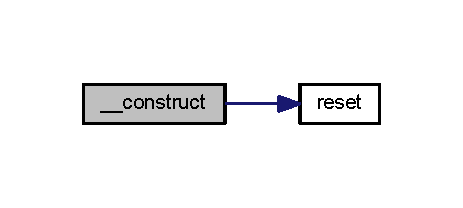
\includegraphics[width=222pt]{class_reversi_anz_a095c5d389db211932136b53f25f39685_cgraph}
\end{center}
\end{figure}
\mbox{\Hypertarget{class_reversi_anz_a421831a265621325e1fdd19aace0c758}\label{class_reversi_anz_a421831a265621325e1fdd19aace0c758}} 
\index{Reversi\+Anz@{Reversi\+Anz}!\+\_\+\+\_\+destruct@{\+\_\+\+\_\+destruct}}
\index{\+\_\+\+\_\+destruct@{\+\_\+\+\_\+destruct}!Reversi\+Anz@{Reversi\+Anz}}
\subsubsection{\texorpdfstring{\+\_\+\+\_\+destruct()}{\_\_destruct()}}
{\footnotesize\ttfamily \+\_\+\+\_\+destruct (\begin{DoxyParamCaption}{ }\end{DoxyParamCaption})}



デストラクタ 

\begin{DoxyReturn}{Returns}
ありません 
\end{DoxyReturn}
\begin{DoxyAuthor}{Author}
Yuta Yoshinaga 
\end{DoxyAuthor}
\begin{DoxyDate}{Date}
2018.\+03.\+02 
\end{DoxyDate}


Definition at line 133 of file Reversi\+Anz.\+php.



\subsection{Member Function Documentation}
\mbox{\Hypertarget{class_reversi_anz_a4a20559544fdf4dcb457e258dc976cf8}\label{class_reversi_anz_a4a20559544fdf4dcb457e258dc976cf8}} 
\index{Reversi\+Anz@{Reversi\+Anz}!reset@{reset}}
\index{reset@{reset}!Reversi\+Anz@{Reversi\+Anz}}
\subsubsection{\texorpdfstring{reset()}{reset()}}
{\footnotesize\ttfamily reset (\begin{DoxyParamCaption}{ }\end{DoxyParamCaption})}



リセット 

\begin{DoxyReturn}{Returns}
ありません 
\end{DoxyReturn}
\begin{DoxyAuthor}{Author}
Yuta Yoshinaga 
\end{DoxyAuthor}
\begin{DoxyDate}{Date}
2018.\+03.\+02 
\end{DoxyDate}


Definition at line 145 of file Reversi\+Anz.\+php.



Referenced by \+\_\+\+\_\+construct().

Here is the caller graph for this function\+:
\nopagebreak
\begin{figure}[H]
\begin{center}
\leavevmode
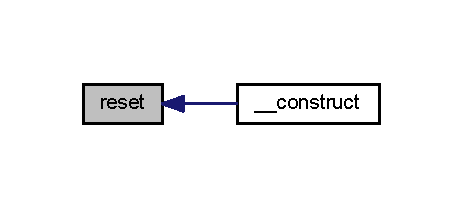
\includegraphics[width=222pt]{class_reversi_anz_a4a20559544fdf4dcb457e258dc976cf8_icgraph}
\end{center}
\end{figure}


The documentation for this class was generated from the following file\+:\begin{DoxyCompactItemize}
\item 
Model/\hyperlink{_reversi_anz_8php}{Reversi\+Anz.\+php}\end{DoxyCompactItemize}

\hypertarget{class_reversi_const}{}\section{Reversi\+Const Class Reference}
\label{class_reversi_const}\index{Reversi\+Const@{Reversi\+Const}}


アプリ設定クラス  




Collaboration diagram for Reversi\+Const\+:
\nopagebreak
\begin{figure}[H]
\begin{center}
\leavevmode
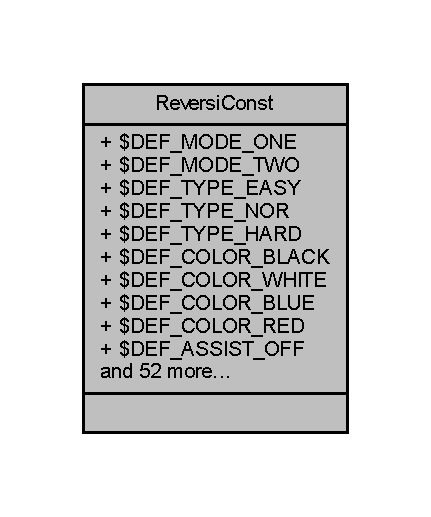
\includegraphics[width=220pt]{class_reversi_const__coll__graph}
\end{center}
\end{figure}
\subsection*{Static Public Attributes}
\begin{DoxyCompactItemize}
\item 
\mbox{\Hypertarget{class_reversi_const_a3ae565ad68b714102079e94a675e2e79}\label{class_reversi_const_a3ae565ad68b714102079e94a675e2e79}} 
static \hyperlink{class_reversi_const_a3ae565ad68b714102079e94a675e2e79}{\$\+D\+E\+F\+\_\+\+M\+O\+D\+E\+\_\+\+O\+NE} = 0
\begin{DoxyCompactList}\small\item\em 一人対戦 \end{DoxyCompactList}\item 
\mbox{\Hypertarget{class_reversi_const_ad6b4696b7c6a13ff0b2bf9971dbfce9e}\label{class_reversi_const_ad6b4696b7c6a13ff0b2bf9971dbfce9e}} 
static \hyperlink{class_reversi_const_ad6b4696b7c6a13ff0b2bf9971dbfce9e}{\$\+D\+E\+F\+\_\+\+M\+O\+D\+E\+\_\+\+T\+WO} = 1
\begin{DoxyCompactList}\small\item\em 二人対戦 \end{DoxyCompactList}\item 
\mbox{\Hypertarget{class_reversi_const_aa7c8b5c0a0cb3962fba2630bd31a3d27}\label{class_reversi_const_aa7c8b5c0a0cb3962fba2630bd31a3d27}} 
static \hyperlink{class_reversi_const_aa7c8b5c0a0cb3962fba2630bd31a3d27}{\$\+D\+E\+F\+\_\+\+T\+Y\+P\+E\+\_\+\+E\+A\+SY} = 0
\begin{DoxyCompactList}\small\item\em C\+PU 弱い \end{DoxyCompactList}\item 
\mbox{\Hypertarget{class_reversi_const_aa41e16eea08a1ac1bee29417b96f56c8}\label{class_reversi_const_aa41e16eea08a1ac1bee29417b96f56c8}} 
static \hyperlink{class_reversi_const_aa41e16eea08a1ac1bee29417b96f56c8}{\$\+D\+E\+F\+\_\+\+T\+Y\+P\+E\+\_\+\+N\+OR} = 1
\begin{DoxyCompactList}\small\item\em C\+PU 普通 \end{DoxyCompactList}\item 
\mbox{\Hypertarget{class_reversi_const_a51a0e47e9e83936aa16a4b7eebdac02f}\label{class_reversi_const_a51a0e47e9e83936aa16a4b7eebdac02f}} 
static \hyperlink{class_reversi_const_a51a0e47e9e83936aa16a4b7eebdac02f}{\$\+D\+E\+F\+\_\+\+T\+Y\+P\+E\+\_\+\+H\+A\+RD} = 2
\begin{DoxyCompactList}\small\item\em C\+PU 強い \end{DoxyCompactList}\item 
\mbox{\Hypertarget{class_reversi_const_ae9bf810749221ae09fbc5c70c2c96b2f}\label{class_reversi_const_ae9bf810749221ae09fbc5c70c2c96b2f}} 
static \hyperlink{class_reversi_const_ae9bf810749221ae09fbc5c70c2c96b2f}{\$\+D\+E\+F\+\_\+\+C\+O\+L\+O\+R\+\_\+\+B\+L\+A\+CK} = 0
\begin{DoxyCompactList}\small\item\em コマ色 黒 \end{DoxyCompactList}\item 
\mbox{\Hypertarget{class_reversi_const_a2e8fc278815f5af6f8a3617570b0f8e3}\label{class_reversi_const_a2e8fc278815f5af6f8a3617570b0f8e3}} 
static \hyperlink{class_reversi_const_a2e8fc278815f5af6f8a3617570b0f8e3}{\$\+D\+E\+F\+\_\+\+C\+O\+L\+O\+R\+\_\+\+W\+H\+I\+TE} = 1
\begin{DoxyCompactList}\small\item\em コマ色 白 \end{DoxyCompactList}\item 
\mbox{\Hypertarget{class_reversi_const_a5de57f1691fb59977a194f038de0ec99}\label{class_reversi_const_a5de57f1691fb59977a194f038de0ec99}} 
static \hyperlink{class_reversi_const_a5de57f1691fb59977a194f038de0ec99}{\$\+D\+E\+F\+\_\+\+A\+S\+S\+I\+S\+T\+\_\+\+O\+FF} = 0
\begin{DoxyCompactList}\small\item\em アシスト O\+FF \end{DoxyCompactList}\item 
\mbox{\Hypertarget{class_reversi_const_ac486ec8951f7327db00d83e6c570cecb}\label{class_reversi_const_ac486ec8951f7327db00d83e6c570cecb}} 
static \hyperlink{class_reversi_const_ac486ec8951f7327db00d83e6c570cecb}{\$\+D\+E\+F\+\_\+\+A\+S\+S\+I\+S\+T\+\_\+\+ON} = 1
\begin{DoxyCompactList}\small\item\em アシスト ON \end{DoxyCompactList}\item 
\mbox{\Hypertarget{class_reversi_const_a8c6962b66e74e00ea5a8d096d69990f9}\label{class_reversi_const_a8c6962b66e74e00ea5a8d096d69990f9}} 
static \hyperlink{class_reversi_const_a8c6962b66e74e00ea5a8d096d69990f9}{\$\+D\+E\+F\+\_\+\+G\+A\+M\+E\+\_\+\+S\+P\+D\+\_\+\+F\+A\+ST} = 0
\begin{DoxyCompactList}\small\item\em ゲームスピード 早い \end{DoxyCompactList}\item 
\mbox{\Hypertarget{class_reversi_const_a193b49bd2c83732144f045f9a50aa33e}\label{class_reversi_const_a193b49bd2c83732144f045f9a50aa33e}} 
static \hyperlink{class_reversi_const_a193b49bd2c83732144f045f9a50aa33e}{\$\+D\+E\+F\+\_\+\+G\+A\+M\+E\+\_\+\+S\+P\+D\+\_\+\+M\+ID} = 1
\begin{DoxyCompactList}\small\item\em ゲームスピード 普通 \end{DoxyCompactList}\item 
\mbox{\Hypertarget{class_reversi_const_a0b3dc06c436244edd6720ad50a6eb673}\label{class_reversi_const_a0b3dc06c436244edd6720ad50a6eb673}} 
static \hyperlink{class_reversi_const_a0b3dc06c436244edd6720ad50a6eb673}{\$\+D\+E\+F\+\_\+\+G\+A\+M\+E\+\_\+\+S\+P\+D\+\_\+\+S\+L\+OW} = 2
\begin{DoxyCompactList}\small\item\em ゲームスピード 遅い \end{DoxyCompactList}\item 
\mbox{\Hypertarget{class_reversi_const_a482c8f8dd0e67619fda3f134ab0a011c}\label{class_reversi_const_a482c8f8dd0e67619fda3f134ab0a011c}} 
static \hyperlink{class_reversi_const_a482c8f8dd0e67619fda3f134ab0a011c}{\$\+D\+E\+F\+\_\+\+G\+A\+M\+E\+\_\+\+S\+P\+D\+\_\+\+F\+A\+S\+T\+\_\+\+V\+AL} = 0
\begin{DoxyCompactList}\small\item\em ゲームスピード 早い \end{DoxyCompactList}\item 
\mbox{\Hypertarget{class_reversi_const_ac370025cba197235c70bb8adf896adf8}\label{class_reversi_const_ac370025cba197235c70bb8adf896adf8}} 
static \hyperlink{class_reversi_const_ac370025cba197235c70bb8adf896adf8}{\$\+D\+E\+F\+\_\+\+G\+A\+M\+E\+\_\+\+S\+P\+D\+\_\+\+M\+I\+D\+\_\+\+V\+AL} = 50
\begin{DoxyCompactList}\small\item\em ゲームスピード 普通 \end{DoxyCompactList}\item 
\mbox{\Hypertarget{class_reversi_const_ab34ef73bafe6b461bd6c352e393428c4}\label{class_reversi_const_ab34ef73bafe6b461bd6c352e393428c4}} 
static \hyperlink{class_reversi_const_ab34ef73bafe6b461bd6c352e393428c4}{\$\+D\+E\+F\+\_\+\+G\+A\+M\+E\+\_\+\+S\+P\+D\+\_\+\+S\+L\+O\+W\+\_\+\+V\+AL} = 100
\begin{DoxyCompactList}\small\item\em ゲームスピード 遅い \end{DoxyCompactList}\item 
\mbox{\Hypertarget{class_reversi_const_a6fa812c8bbe57a64fd92223fd3b71086}\label{class_reversi_const_a6fa812c8bbe57a64fd92223fd3b71086}} 
static \hyperlink{class_reversi_const_a6fa812c8bbe57a64fd92223fd3b71086}{\$\+D\+E\+F\+\_\+\+G\+A\+M\+E\+\_\+\+S\+P\+D\+\_\+\+F\+A\+S\+T\+\_\+\+V\+A\+L2} = 0
\begin{DoxyCompactList}\small\item\em ゲームスピード 早い \end{DoxyCompactList}\item 
\mbox{\Hypertarget{class_reversi_const_a016bb70e8fca576083b82f70c5abf022}\label{class_reversi_const_a016bb70e8fca576083b82f70c5abf022}} 
static \hyperlink{class_reversi_const_a016bb70e8fca576083b82f70c5abf022}{\$\+D\+E\+F\+\_\+\+G\+A\+M\+E\+\_\+\+S\+P\+D\+\_\+\+M\+I\+D\+\_\+\+V\+A\+L2} = 500
\begin{DoxyCompactList}\small\item\em ゲームスピード 普通 \end{DoxyCompactList}\item 
\mbox{\Hypertarget{class_reversi_const_a6742adf1a0780356fd92b8a18c1710c8}\label{class_reversi_const_a6742adf1a0780356fd92b8a18c1710c8}} 
static \hyperlink{class_reversi_const_a6742adf1a0780356fd92b8a18c1710c8}{\$\+D\+E\+F\+\_\+\+G\+A\+M\+E\+\_\+\+S\+P\+D\+\_\+\+S\+L\+O\+W\+\_\+\+V\+A\+L2} = 1000
\begin{DoxyCompactList}\small\item\em ゲームスピード 遅い \end{DoxyCompactList}\item 
\mbox{\Hypertarget{class_reversi_const_a61944ae88b15f2b7a1e0fafa6427b1d9}\label{class_reversi_const_a61944ae88b15f2b7a1e0fafa6427b1d9}} 
static \hyperlink{class_reversi_const_a61944ae88b15f2b7a1e0fafa6427b1d9}{\$\+D\+E\+F\+\_\+\+E\+N\+D\+\_\+\+A\+N\+I\+M\+\_\+\+O\+FF} = 0
\begin{DoxyCompactList}\small\item\em 終了アニメーション O\+FF \end{DoxyCompactList}\item 
\mbox{\Hypertarget{class_reversi_const_ad0da61a2d5650bdefb8db60d69d686ed}\label{class_reversi_const_ad0da61a2d5650bdefb8db60d69d686ed}} 
static \hyperlink{class_reversi_const_ad0da61a2d5650bdefb8db60d69d686ed}{\$\+D\+E\+F\+\_\+\+E\+N\+D\+\_\+\+A\+N\+I\+M\+\_\+\+ON} = 1
\begin{DoxyCompactList}\small\item\em 終了アニメーション ON \end{DoxyCompactList}\item 
\mbox{\Hypertarget{class_reversi_const_a2dd1b7bb9f8733961e1b526d977bf64e}\label{class_reversi_const_a2dd1b7bb9f8733961e1b526d977bf64e}} 
static \hyperlink{class_reversi_const_a2dd1b7bb9f8733961e1b526d977bf64e}{\$\+D\+E\+F\+\_\+\+M\+A\+S\+U\+\_\+\+C\+N\+T\+\_\+6} = 0
\begin{DoxyCompactList}\small\item\em マス縦横6 \end{DoxyCompactList}\item 
\mbox{\Hypertarget{class_reversi_const_a3768b1d96ac805b361ba9c1ee64b68c3}\label{class_reversi_const_a3768b1d96ac805b361ba9c1ee64b68c3}} 
static \hyperlink{class_reversi_const_a3768b1d96ac805b361ba9c1ee64b68c3}{\$\+D\+E\+F\+\_\+\+M\+A\+S\+U\+\_\+\+C\+N\+T\+\_\+8} = 1
\begin{DoxyCompactList}\small\item\em マス縦横8 \end{DoxyCompactList}\item 
\mbox{\Hypertarget{class_reversi_const_a229d8a2af11898150ee33606343c7deb}\label{class_reversi_const_a229d8a2af11898150ee33606343c7deb}} 
static \hyperlink{class_reversi_const_a229d8a2af11898150ee33606343c7deb}{\$\+D\+E\+F\+\_\+\+M\+A\+S\+U\+\_\+\+C\+N\+T\+\_\+10} = 2
\begin{DoxyCompactList}\small\item\em マス縦横10 \end{DoxyCompactList}\item 
\mbox{\Hypertarget{class_reversi_const_a9334dcfbdeb613964a57a2aa7dfb0622}\label{class_reversi_const_a9334dcfbdeb613964a57a2aa7dfb0622}} 
static \hyperlink{class_reversi_const_a9334dcfbdeb613964a57a2aa7dfb0622}{\$\+D\+E\+F\+\_\+\+M\+A\+S\+U\+\_\+\+C\+N\+T\+\_\+12} = 3
\begin{DoxyCompactList}\small\item\em マス縦横12 \end{DoxyCompactList}\item 
\mbox{\Hypertarget{class_reversi_const_a907a12a72eda65bd4dcb63328fe8541d}\label{class_reversi_const_a907a12a72eda65bd4dcb63328fe8541d}} 
static \hyperlink{class_reversi_const_a907a12a72eda65bd4dcb63328fe8541d}{\$\+D\+E\+F\+\_\+\+M\+A\+S\+U\+\_\+\+C\+N\+T\+\_\+14} = 4
\begin{DoxyCompactList}\small\item\em マス縦横14 \end{DoxyCompactList}\item 
\mbox{\Hypertarget{class_reversi_const_a05fa5ab5e893a290425bdfa990db4105}\label{class_reversi_const_a05fa5ab5e893a290425bdfa990db4105}} 
static \hyperlink{class_reversi_const_a05fa5ab5e893a290425bdfa990db4105}{\$\+D\+E\+F\+\_\+\+M\+A\+S\+U\+\_\+\+C\+N\+T\+\_\+16} = 5
\begin{DoxyCompactList}\small\item\em マス縦横16 \end{DoxyCompactList}\item 
\mbox{\Hypertarget{class_reversi_const_ac4cdee79d87ba30c9e1ad5f76763a3c9}\label{class_reversi_const_ac4cdee79d87ba30c9e1ad5f76763a3c9}} 
static \hyperlink{class_reversi_const_ac4cdee79d87ba30c9e1ad5f76763a3c9}{\$\+D\+E\+F\+\_\+\+M\+A\+S\+U\+\_\+\+C\+N\+T\+\_\+18} = 6
\begin{DoxyCompactList}\small\item\em マス縦横18 \end{DoxyCompactList}\item 
\mbox{\Hypertarget{class_reversi_const_a45a5b589a2b3ac2af7d0e5d638791ffc}\label{class_reversi_const_a45a5b589a2b3ac2af7d0e5d638791ffc}} 
static \hyperlink{class_reversi_const_a45a5b589a2b3ac2af7d0e5d638791ffc}{\$\+D\+E\+F\+\_\+\+M\+A\+S\+U\+\_\+\+C\+N\+T\+\_\+20} = 7
\begin{DoxyCompactList}\small\item\em マス縦横20 \end{DoxyCompactList}\item 
\mbox{\Hypertarget{class_reversi_const_a610ea7766cdf77e22ee36f195efc73a1}\label{class_reversi_const_a610ea7766cdf77e22ee36f195efc73a1}} 
static \hyperlink{class_reversi_const_a610ea7766cdf77e22ee36f195efc73a1}{\$\+D\+E\+F\+\_\+\+M\+A\+S\+U\+\_\+\+C\+N\+T\+\_\+6\+\_\+\+V\+AL} = 6
\begin{DoxyCompactList}\small\item\em マス縦横6 \end{DoxyCompactList}\item 
\mbox{\Hypertarget{class_reversi_const_a0ae1ba6bd2dfeac3259b9b6afaaed4d2}\label{class_reversi_const_a0ae1ba6bd2dfeac3259b9b6afaaed4d2}} 
static \hyperlink{class_reversi_const_a0ae1ba6bd2dfeac3259b9b6afaaed4d2}{\$\+D\+E\+F\+\_\+\+M\+A\+S\+U\+\_\+\+C\+N\+T\+\_\+8\+\_\+\+V\+AL} = 8
\begin{DoxyCompactList}\small\item\em マス縦横8 \end{DoxyCompactList}\item 
\mbox{\Hypertarget{class_reversi_const_a711060d4402e0e7f4e5ea5f9c3d0e407}\label{class_reversi_const_a711060d4402e0e7f4e5ea5f9c3d0e407}} 
static \hyperlink{class_reversi_const_a711060d4402e0e7f4e5ea5f9c3d0e407}{\$\+D\+E\+F\+\_\+\+M\+A\+S\+U\+\_\+\+C\+N\+T\+\_\+10\+\_\+\+V\+AL} = 10
\begin{DoxyCompactList}\small\item\em マス縦横10 \end{DoxyCompactList}\item 
\mbox{\Hypertarget{class_reversi_const_a78b9d9b338b9f7293eb44fbc88b44a7e}\label{class_reversi_const_a78b9d9b338b9f7293eb44fbc88b44a7e}} 
static \hyperlink{class_reversi_const_a78b9d9b338b9f7293eb44fbc88b44a7e}{\$\+D\+E\+F\+\_\+\+M\+A\+S\+U\+\_\+\+C\+N\+T\+\_\+12\+\_\+\+V\+AL} = 12
\begin{DoxyCompactList}\small\item\em マス縦横12 \end{DoxyCompactList}\item 
\mbox{\Hypertarget{class_reversi_const_a0fa489876583e3c7afae744b9c4e2fd1}\label{class_reversi_const_a0fa489876583e3c7afae744b9c4e2fd1}} 
static \hyperlink{class_reversi_const_a0fa489876583e3c7afae744b9c4e2fd1}{\$\+D\+E\+F\+\_\+\+M\+A\+S\+U\+\_\+\+C\+N\+T\+\_\+14\+\_\+\+V\+AL} = 14
\begin{DoxyCompactList}\small\item\em マス縦横14 \end{DoxyCompactList}\item 
\mbox{\Hypertarget{class_reversi_const_ab29f123aba64c8d34c895ef700ad9c6b}\label{class_reversi_const_ab29f123aba64c8d34c895ef700ad9c6b}} 
static \hyperlink{class_reversi_const_ab29f123aba64c8d34c895ef700ad9c6b}{\$\+D\+E\+F\+\_\+\+M\+A\+S\+U\+\_\+\+C\+N\+T\+\_\+16\+\_\+\+V\+AL} = 16
\begin{DoxyCompactList}\small\item\em マス縦横16 \end{DoxyCompactList}\item 
\mbox{\Hypertarget{class_reversi_const_a4232cfd29ffc57b86911fef7b04ba056}\label{class_reversi_const_a4232cfd29ffc57b86911fef7b04ba056}} 
static \hyperlink{class_reversi_const_a4232cfd29ffc57b86911fef7b04ba056}{\$\+D\+E\+F\+\_\+\+M\+A\+S\+U\+\_\+\+C\+N\+T\+\_\+18\+\_\+\+V\+AL} = 18
\begin{DoxyCompactList}\small\item\em マス縦横18 \end{DoxyCompactList}\item 
\mbox{\Hypertarget{class_reversi_const_ac987dbaa8da3871c3c35743aa26be89a}\label{class_reversi_const_ac987dbaa8da3871c3c35743aa26be89a}} 
static \hyperlink{class_reversi_const_ac987dbaa8da3871c3c35743aa26be89a}{\$\+D\+E\+F\+\_\+\+M\+A\+S\+U\+\_\+\+C\+N\+T\+\_\+20\+\_\+\+V\+AL} = 20
\begin{DoxyCompactList}\small\item\em マス縦横20 \end{DoxyCompactList}\item 
\mbox{\Hypertarget{class_reversi_const_ac57be288e8fbde4a2e620609ce02925b}\label{class_reversi_const_ac57be288e8fbde4a2e620609ce02925b}} 
static \hyperlink{class_reversi_const_ac57be288e8fbde4a2e620609ce02925b}{\$\+D\+E\+F\+\_\+\+M\+A\+S\+U\+\_\+\+C\+N\+T\+\_\+\+M\+A\+X\+\_\+\+V\+AL} = 20
\begin{DoxyCompactList}\small\item\em マス縦横最大 \end{DoxyCompactList}\item 
\mbox{\Hypertarget{class_reversi_const_aafea7fe2f84562cd883a884285ded09c}\label{class_reversi_const_aafea7fe2f84562cd883a884285ded09c}} 
static \hyperlink{class_reversi_const_aafea7fe2f84562cd883a884285ded09c}{\$\+R\+E\+V\+E\+R\+S\+I\+\_\+\+S\+T\+S\+\_\+\+N\+O\+NE} = 0
\begin{DoxyCompactList}\small\item\em コマ無し \end{DoxyCompactList}\item 
\mbox{\Hypertarget{class_reversi_const_a02fbb6f48064d833739f11e6c166d342}\label{class_reversi_const_a02fbb6f48064d833739f11e6c166d342}} 
static \hyperlink{class_reversi_const_a02fbb6f48064d833739f11e6c166d342}{\$\+R\+E\+V\+E\+R\+S\+I\+\_\+\+S\+T\+S\+\_\+\+B\+L\+A\+CK} = 1
\begin{DoxyCompactList}\small\item\em 黒 \end{DoxyCompactList}\item 
\mbox{\Hypertarget{class_reversi_const_a7d7cce1f800aec960277bcfafe5eb9c2}\label{class_reversi_const_a7d7cce1f800aec960277bcfafe5eb9c2}} 
static \hyperlink{class_reversi_const_a7d7cce1f800aec960277bcfafe5eb9c2}{\$\+R\+E\+V\+E\+R\+S\+I\+\_\+\+S\+T\+S\+\_\+\+W\+H\+I\+TE} = 2
\begin{DoxyCompactList}\small\item\em 白 \end{DoxyCompactList}\item 
\mbox{\Hypertarget{class_reversi_const_aa0e0852db16c70abcbf8b55b9bccfedc}\label{class_reversi_const_aa0e0852db16c70abcbf8b55b9bccfedc}} 
static \hyperlink{class_reversi_const_aa0e0852db16c70abcbf8b55b9bccfedc}{\$\+R\+E\+V\+E\+R\+S\+I\+\_\+\+S\+T\+S\+\_\+\+M\+IN} = 0
\begin{DoxyCompactList}\small\item\em ステータス最小値 \end{DoxyCompactList}\item 
\mbox{\Hypertarget{class_reversi_const_abe1166d89a529d2a7f9bd235e14e9b64}\label{class_reversi_const_abe1166d89a529d2a7f9bd235e14e9b64}} 
static \hyperlink{class_reversi_const_abe1166d89a529d2a7f9bd235e14e9b64}{\$\+R\+E\+V\+E\+R\+S\+I\+\_\+\+S\+T\+S\+\_\+\+M\+AX} = 2
\begin{DoxyCompactList}\small\item\em ステータス最大値 \end{DoxyCompactList}\item 
\mbox{\Hypertarget{class_reversi_const_a1346cd55e42c8ed965831ea2eba3e26f}\label{class_reversi_const_a1346cd55e42c8ed965831ea2eba3e26f}} 
static \hyperlink{class_reversi_const_a1346cd55e42c8ed965831ea2eba3e26f}{\$\+R\+E\+V\+E\+R\+S\+I\+\_\+\+M\+A\+S\+U\+\_\+\+C\+NT} = 8
\begin{DoxyCompactList}\small\item\em 縦横マス数 \end{DoxyCompactList}\item 
\mbox{\Hypertarget{class_reversi_const_af2cfd84202bbe2dfb22250be713aea65}\label{class_reversi_const_af2cfd84202bbe2dfb22250be713aea65}} 
static \hyperlink{class_reversi_const_af2cfd84202bbe2dfb22250be713aea65}{\$\+L\+C\+\_\+\+M\+S\+G\+\_\+\+D\+R\+AW} = 0
\begin{DoxyCompactList}\small\item\em マス描画 \end{DoxyCompactList}\item 
\mbox{\Hypertarget{class_reversi_const_af1e58340af7831eaf0458fe771f51119}\label{class_reversi_const_af1e58340af7831eaf0458fe771f51119}} 
static \hyperlink{class_reversi_const_af1e58340af7831eaf0458fe771f51119}{\$\+L\+C\+\_\+\+M\+S\+G\+\_\+\+E\+R\+A\+SE} = 1
\begin{DoxyCompactList}\small\item\em マス消去 \end{DoxyCompactList}\item 
\mbox{\Hypertarget{class_reversi_const_a522738851ab060cd14ce3ffa1618000e}\label{class_reversi_const_a522738851ab060cd14ce3ffa1618000e}} 
static \hyperlink{class_reversi_const_a522738851ab060cd14ce3ffa1618000e}{\$\+L\+C\+\_\+\+M\+S\+G\+\_\+\+D\+R\+A\+W\+\_\+\+I\+N\+FO} = 2
\begin{DoxyCompactList}\small\item\em マス情報描画 \end{DoxyCompactList}\item 
\mbox{\Hypertarget{class_reversi_const_a8ad50be0a297eea01df37fd8ba20d353}\label{class_reversi_const_a8ad50be0a297eea01df37fd8ba20d353}} 
static \hyperlink{class_reversi_const_a8ad50be0a297eea01df37fd8ba20d353}{\$\+L\+C\+\_\+\+M\+S\+G\+\_\+\+E\+R\+A\+S\+E\+\_\+\+I\+N\+FO} = 3
\begin{DoxyCompactList}\small\item\em マス情報消去 \end{DoxyCompactList}\item 
\mbox{\Hypertarget{class_reversi_const_a3074235c57b33980f06e0ec357302e87}\label{class_reversi_const_a3074235c57b33980f06e0ec357302e87}} 
static \hyperlink{class_reversi_const_a3074235c57b33980f06e0ec357302e87}{\$\+L\+C\+\_\+\+M\+S\+G\+\_\+\+D\+R\+A\+W\+\_\+\+A\+LL} = 4
\begin{DoxyCompactList}\small\item\em 全マス描画 \end{DoxyCompactList}\item 
\mbox{\Hypertarget{class_reversi_const_a6c2ec1c0d689ebe57d1ccd9eb9589da8}\label{class_reversi_const_a6c2ec1c0d689ebe57d1ccd9eb9589da8}} 
static \hyperlink{class_reversi_const_a6c2ec1c0d689ebe57d1ccd9eb9589da8}{\$\+L\+C\+\_\+\+M\+S\+G\+\_\+\+E\+R\+A\+S\+E\+\_\+\+A\+LL} = 5
\begin{DoxyCompactList}\small\item\em 全マス消去 \end{DoxyCompactList}\item 
\mbox{\Hypertarget{class_reversi_const_a878b3d361d535e996827103efecdbfa3}\label{class_reversi_const_a878b3d361d535e996827103efecdbfa3}} 
static \hyperlink{class_reversi_const_a878b3d361d535e996827103efecdbfa3}{\$\+L\+C\+\_\+\+M\+S\+G\+\_\+\+D\+R\+A\+W\+\_\+\+I\+N\+F\+O\+\_\+\+A\+LL} = 6
\begin{DoxyCompactList}\small\item\em 全マス情報描画 \end{DoxyCompactList}\item 
\mbox{\Hypertarget{class_reversi_const_ad45d7e4a301c2cfa4b0a12ddfa373425}\label{class_reversi_const_ad45d7e4a301c2cfa4b0a12ddfa373425}} 
static \hyperlink{class_reversi_const_ad45d7e4a301c2cfa4b0a12ddfa373425}{\$\+L\+C\+\_\+\+M\+S\+G\+\_\+\+E\+R\+A\+S\+E\+\_\+\+I\+N\+F\+O\+\_\+\+A\+LL} = 7
\begin{DoxyCompactList}\small\item\em 全マス情報消去 \end{DoxyCompactList}\item 
\mbox{\Hypertarget{class_reversi_const_ac5fc5dc1425fd1c238faf57d0d3d0510}\label{class_reversi_const_ac5fc5dc1425fd1c238faf57d0d3d0510}} 
static \hyperlink{class_reversi_const_ac5fc5dc1425fd1c238faf57d0d3d0510}{\$\+L\+C\+\_\+\+M\+S\+G\+\_\+\+D\+R\+A\+W\+\_\+\+E\+ND} = 8
\begin{DoxyCompactList}\small\item\em 描画終わり \end{DoxyCompactList}\item 
\mbox{\Hypertarget{class_reversi_const_a6acbb83271876a127eadc9eb7cb425cd}\label{class_reversi_const_a6acbb83271876a127eadc9eb7cb425cd}} 
static \hyperlink{class_reversi_const_a6acbb83271876a127eadc9eb7cb425cd}{\$\+L\+C\+\_\+\+M\+S\+G\+\_\+\+C\+U\+R\+\_\+\+C\+OL} = 9
\begin{DoxyCompactList}\small\item\em 現在の色 \end{DoxyCompactList}\item 
\mbox{\Hypertarget{class_reversi_const_aca271c05f15761f26583cfb884e5fc20}\label{class_reversi_const_aca271c05f15761f26583cfb884e5fc20}} 
static \hyperlink{class_reversi_const_aca271c05f15761f26583cfb884e5fc20}{\$\+L\+C\+\_\+\+M\+S\+G\+\_\+\+C\+U\+R\+\_\+\+C\+O\+L\+\_\+\+E\+R\+A\+SE} = 10
\begin{DoxyCompactList}\small\item\em 現在の色消去 \end{DoxyCompactList}\item 
\mbox{\Hypertarget{class_reversi_const_ac3301c4726ee8acb3d5f2810d9e0559e}\label{class_reversi_const_ac3301c4726ee8acb3d5f2810d9e0559e}} 
static \hyperlink{class_reversi_const_ac3301c4726ee8acb3d5f2810d9e0559e}{\$\+L\+C\+\_\+\+M\+S\+G\+\_\+\+C\+U\+R\+\_\+\+S\+TS} = 11
\begin{DoxyCompactList}\small\item\em 現在のステータス \end{DoxyCompactList}\item 
\mbox{\Hypertarget{class_reversi_const_a820a0338238bbd1f21c29b63aadbf2c8}\label{class_reversi_const_a820a0338238bbd1f21c29b63aadbf2c8}} 
static \hyperlink{class_reversi_const_a820a0338238bbd1f21c29b63aadbf2c8}{\$\+L\+C\+\_\+\+M\+S\+G\+\_\+\+C\+U\+R\+\_\+\+S\+T\+S\+\_\+\+E\+R\+A\+SE} = 12
\begin{DoxyCompactList}\small\item\em 現在のステータス消去 \end{DoxyCompactList}\item 
\mbox{\Hypertarget{class_reversi_const_a11bb64ddfba78520e7864e0fe8aa89d1}\label{class_reversi_const_a11bb64ddfba78520e7864e0fe8aa89d1}} 
static \hyperlink{class_reversi_const_a11bb64ddfba78520e7864e0fe8aa89d1}{\$\+L\+C\+\_\+\+M\+S\+G\+\_\+\+M\+S\+G\+\_\+\+D\+LG} = 13
\begin{DoxyCompactList}\small\item\em メッセージダイアログ \end{DoxyCompactList}\item 
\mbox{\Hypertarget{class_reversi_const_ab474e9969881fca250d354949405d7d8}\label{class_reversi_const_ab474e9969881fca250d354949405d7d8}} 
static \hyperlink{class_reversi_const_ab474e9969881fca250d354949405d7d8}{\$\+L\+C\+\_\+\+M\+S\+G\+\_\+\+D\+R\+A\+W\+\_\+\+A\+L\+L\+\_\+\+R\+E\+S\+ET} = 14
\begin{DoxyCompactList}\small\item\em 全マスビットマップインスタンスクリア \end{DoxyCompactList}\end{DoxyCompactItemize}


\subsection{Detailed Description}
アプリ設定クラス 

Definition at line 25 of file Reversi\+Const.\+php.



The documentation for this class was generated from the following file\+:\begin{DoxyCompactItemize}
\item 
Model/\hyperlink{_reversi_const_8php}{Reversi\+Const.\+php}\end{DoxyCompactItemize}

\hypertarget{class_reversi_history}{}\section{Reversi\+History Class Reference}
\label{class_reversi_history}\index{Reversi\+History@{Reversi\+History}}


リバーシ履歴クラス  




Collaboration diagram for Reversi\+History\+:
\nopagebreak
\begin{figure}[H]
\begin{center}
\leavevmode
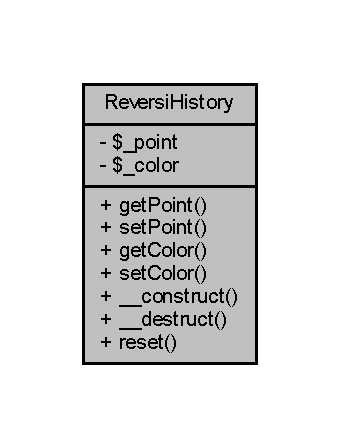
\includegraphics[width=163pt]{class_reversi_history__coll__graph}
\end{center}
\end{figure}
\subsection*{Public Member Functions}
\begin{DoxyCompactItemize}
\item 
\mbox{\Hypertarget{class_reversi_history_a07a3d9858b0eee18a3aeed77197ce9f3}\label{class_reversi_history_a07a3d9858b0eee18a3aeed77197ce9f3}} 
{\bfseries get\+Point} ()
\item 
\mbox{\Hypertarget{class_reversi_history_a90f70a3f275795c6cd5e7f5f8b65727d}\label{class_reversi_history_a90f70a3f275795c6cd5e7f5f8b65727d}} 
{\bfseries set\+Point} (\$\+\_\+point)
\item 
\mbox{\Hypertarget{class_reversi_history_aa8642511e4effd1b9ff80c64ff788cfd}\label{class_reversi_history_aa8642511e4effd1b9ff80c64ff788cfd}} 
{\bfseries get\+Color} ()
\item 
\mbox{\Hypertarget{class_reversi_history_abfdefaf70a84d60cef2aa34422b74242}\label{class_reversi_history_abfdefaf70a84d60cef2aa34422b74242}} 
{\bfseries set\+Color} (\$\+\_\+color)
\item 
\hyperlink{class_reversi_history_a095c5d389db211932136b53f25f39685}{\+\_\+\+\_\+construct} ()
\begin{DoxyCompactList}\small\item\em コンストラクタ \end{DoxyCompactList}\item 
\hyperlink{class_reversi_history_a421831a265621325e1fdd19aace0c758}{\+\_\+\+\_\+destruct} ()
\begin{DoxyCompactList}\small\item\em デストラクタ \end{DoxyCompactList}\item 
\hyperlink{class_reversi_history_a4a20559544fdf4dcb457e258dc976cf8}{reset} ()
\begin{DoxyCompactList}\small\item\em リセット \end{DoxyCompactList}\end{DoxyCompactItemize}
\subsection*{Private Attributes}
\begin{DoxyCompactItemize}
\item 
\mbox{\Hypertarget{class_reversi_history_a462074d128a4ffaebbbf2bfad75a528d}\label{class_reversi_history_a462074d128a4ffaebbbf2bfad75a528d}} 
\hyperlink{class_reversi_history_a462074d128a4ffaebbbf2bfad75a528d}{\$\+\_\+point}
\begin{DoxyCompactList}\small\item\em ポイント \end{DoxyCompactList}\item 
\mbox{\Hypertarget{class_reversi_history_a924042a4565897f645c836c1e710b807}\label{class_reversi_history_a924042a4565897f645c836c1e710b807}} 
\hyperlink{class_reversi_history_a924042a4565897f645c836c1e710b807}{\$\+\_\+color}
\begin{DoxyCompactList}\small\item\em 色 \end{DoxyCompactList}\end{DoxyCompactItemize}


\subsection{Detailed Description}
リバーシ履歴クラス 

Definition at line 27 of file Reversi\+History.\+php.



\subsection{Constructor \& Destructor Documentation}
\mbox{\Hypertarget{class_reversi_history_a095c5d389db211932136b53f25f39685}\label{class_reversi_history_a095c5d389db211932136b53f25f39685}} 
\index{Reversi\+History@{Reversi\+History}!\+\_\+\+\_\+construct@{\+\_\+\+\_\+construct}}
\index{\+\_\+\+\_\+construct@{\+\_\+\+\_\+construct}!Reversi\+History@{Reversi\+History}}
\subsubsection{\texorpdfstring{\+\_\+\+\_\+construct()}{\_\_construct()}}
{\footnotesize\ttfamily \+\_\+\+\_\+construct (\begin{DoxyParamCaption}{ }\end{DoxyParamCaption})}



コンストラクタ 

\begin{DoxyReturn}{Returns}
ありません 
\end{DoxyReturn}
\begin{DoxyAuthor}{Author}
Yuta Yoshinaga 
\end{DoxyAuthor}
\begin{DoxyDate}{Date}
2018.\+03.\+02 
\end{DoxyDate}


Definition at line 50 of file Reversi\+History.\+php.

Here is the call graph for this function\+:
\nopagebreak
\begin{figure}[H]
\begin{center}
\leavevmode
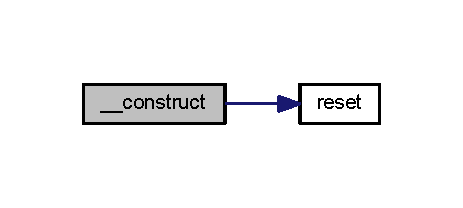
\includegraphics[width=222pt]{class_reversi_history_a095c5d389db211932136b53f25f39685_cgraph}
\end{center}
\end{figure}
\mbox{\Hypertarget{class_reversi_history_a421831a265621325e1fdd19aace0c758}\label{class_reversi_history_a421831a265621325e1fdd19aace0c758}} 
\index{Reversi\+History@{Reversi\+History}!\+\_\+\+\_\+destruct@{\+\_\+\+\_\+destruct}}
\index{\+\_\+\+\_\+destruct@{\+\_\+\+\_\+destruct}!Reversi\+History@{Reversi\+History}}
\subsubsection{\texorpdfstring{\+\_\+\+\_\+destruct()}{\_\_destruct()}}
{\footnotesize\ttfamily \+\_\+\+\_\+destruct (\begin{DoxyParamCaption}{ }\end{DoxyParamCaption})}



デストラクタ 

\begin{DoxyReturn}{Returns}
ありません 
\end{DoxyReturn}
\begin{DoxyAuthor}{Author}
Yuta Yoshinaga 
\end{DoxyAuthor}
\begin{DoxyDate}{Date}
2018.\+03.\+02 
\end{DoxyDate}


Definition at line 64 of file Reversi\+History.\+php.



\subsection{Member Function Documentation}
\mbox{\Hypertarget{class_reversi_history_a4a20559544fdf4dcb457e258dc976cf8}\label{class_reversi_history_a4a20559544fdf4dcb457e258dc976cf8}} 
\index{Reversi\+History@{Reversi\+History}!reset@{reset}}
\index{reset@{reset}!Reversi\+History@{Reversi\+History}}
\subsubsection{\texorpdfstring{reset()}{reset()}}
{\footnotesize\ttfamily reset (\begin{DoxyParamCaption}{ }\end{DoxyParamCaption})}



リセット 

\begin{DoxyReturn}{Returns}
ありません 
\end{DoxyReturn}
\begin{DoxyAuthor}{Author}
Yuta Yoshinaga 
\end{DoxyAuthor}
\begin{DoxyDate}{Date}
2018.\+03.\+02 
\end{DoxyDate}


Definition at line 76 of file Reversi\+History.\+php.



Referenced by \+\_\+\+\_\+construct().

Here is the caller graph for this function\+:
\nopagebreak
\begin{figure}[H]
\begin{center}
\leavevmode
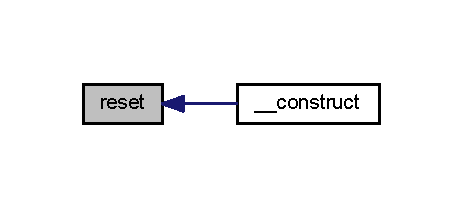
\includegraphics[width=222pt]{class_reversi_history_a4a20559544fdf4dcb457e258dc976cf8_icgraph}
\end{center}
\end{figure}


The documentation for this class was generated from the following file\+:\begin{DoxyCompactItemize}
\item 
Model/\hyperlink{_reversi_history_8php}{Reversi\+History.\+php}\end{DoxyCompactItemize}

\hypertarget{class_reversi_play}{}\section{Reversi\+Play Class Reference}
\label{class_reversi_play}\index{Reversi\+Play@{Reversi\+Play}}


リバーシプレイクラス  




Collaboration diagram for Reversi\+Play\+:
\nopagebreak
\begin{figure}[H]
\begin{center}
\leavevmode
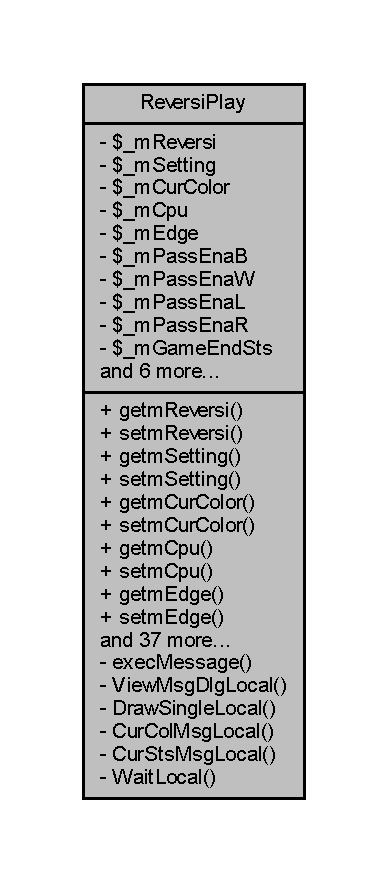
\includegraphics[width=186pt]{class_reversi_play__coll__graph}
\end{center}
\end{figure}
\subsection*{Public Member Functions}
\begin{DoxyCompactItemize}
\item 
\mbox{\Hypertarget{class_reversi_play_a88069db3b0a3146d0dcc7771410fd895}\label{class_reversi_play_a88069db3b0a3146d0dcc7771410fd895}} 
{\bfseries getm\+Reversi} ()
\item 
\mbox{\Hypertarget{class_reversi_play_a39c396a4fad5f72261d628f5018f268e}\label{class_reversi_play_a39c396a4fad5f72261d628f5018f268e}} 
{\bfseries setm\+Reversi} (\$\+\_\+m\+Reversi)
\item 
\mbox{\Hypertarget{class_reversi_play_a1c2a765d1aefb409fd3e39688140ba21}\label{class_reversi_play_a1c2a765d1aefb409fd3e39688140ba21}} 
{\bfseries getm\+Setting} ()
\item 
\mbox{\Hypertarget{class_reversi_play_a0f01407d5c9237e3bc10e9317dc3d3aa}\label{class_reversi_play_a0f01407d5c9237e3bc10e9317dc3d3aa}} 
{\bfseries setm\+Setting} (\$\+\_\+m\+Setting)
\item 
\mbox{\Hypertarget{class_reversi_play_a45b05e31f8be40c86e4e23948a05771b}\label{class_reversi_play_a45b05e31f8be40c86e4e23948a05771b}} 
{\bfseries getm\+Cur\+Color} ()
\item 
\mbox{\Hypertarget{class_reversi_play_a94119d2910f42dd78f7039f9d848c06c}\label{class_reversi_play_a94119d2910f42dd78f7039f9d848c06c}} 
{\bfseries setm\+Cur\+Color} (\$\+\_\+m\+Cur\+Color)
\item 
\mbox{\Hypertarget{class_reversi_play_ac0571dfe3aa8b4f2d83ffda38eff9570}\label{class_reversi_play_ac0571dfe3aa8b4f2d83ffda38eff9570}} 
{\bfseries getm\+Cpu} ()
\item 
\mbox{\Hypertarget{class_reversi_play_a5cc7789f378a0767a17d8eddf5910005}\label{class_reversi_play_a5cc7789f378a0767a17d8eddf5910005}} 
{\bfseries setm\+Cpu} (\$\+\_\+m\+Cpu)
\item 
\mbox{\Hypertarget{class_reversi_play_ada26f3681011904528f3e3dfed9f17df}\label{class_reversi_play_ada26f3681011904528f3e3dfed9f17df}} 
{\bfseries getm\+Edge} ()
\item 
\mbox{\Hypertarget{class_reversi_play_a6888b14f2d98174e4a2e5886a902a8b0}\label{class_reversi_play_a6888b14f2d98174e4a2e5886a902a8b0}} 
{\bfseries setm\+Edge} (\$\+\_\+m\+Edge)
\item 
\mbox{\Hypertarget{class_reversi_play_abc896b77f0242458a6137a1f5c3501ed}\label{class_reversi_play_abc896b77f0242458a6137a1f5c3501ed}} 
{\bfseries getm\+Pass\+EnaB} ()
\item 
\mbox{\Hypertarget{class_reversi_play_a815a48f29873f7cbd68e01463debced0}\label{class_reversi_play_a815a48f29873f7cbd68e01463debced0}} 
{\bfseries setm\+Pass\+EnaB} (\$\+\_\+m\+Pass\+EnaB)
\item 
\mbox{\Hypertarget{class_reversi_play_a9046f25adb88265698a1a177fc777a62}\label{class_reversi_play_a9046f25adb88265698a1a177fc777a62}} 
{\bfseries getm\+Pass\+EnaW} ()
\item 
\mbox{\Hypertarget{class_reversi_play_a198f8569bdaae8b5065a4ff5833e3dda}\label{class_reversi_play_a198f8569bdaae8b5065a4ff5833e3dda}} 
{\bfseries setm\+Pass\+EnaW} (\$\+\_\+m\+Pass\+EnaW)
\item 
\mbox{\Hypertarget{class_reversi_play_a8c52b516d55ee5ad328b7c652818b05a}\label{class_reversi_play_a8c52b516d55ee5ad328b7c652818b05a}} 
{\bfseries getm\+Pass\+EnaL} ()
\item 
\mbox{\Hypertarget{class_reversi_play_a8cf65e1b5ffed9da0890ff2c21362a7e}\label{class_reversi_play_a8cf65e1b5ffed9da0890ff2c21362a7e}} 
{\bfseries setm\+Pass\+EnaL} (\$\+\_\+m\+Pass\+EnaL)
\item 
\mbox{\Hypertarget{class_reversi_play_a61b5d71d69e8e3641812c82ac98c9587}\label{class_reversi_play_a61b5d71d69e8e3641812c82ac98c9587}} 
{\bfseries getm\+Pass\+EnaR} ()
\item 
\mbox{\Hypertarget{class_reversi_play_a8dbcf6f29086358b5b1563919bf54b96}\label{class_reversi_play_a8dbcf6f29086358b5b1563919bf54b96}} 
{\bfseries setm\+Pass\+EnaR} (\$\+\_\+m\+Pass\+EnaR)
\item 
\mbox{\Hypertarget{class_reversi_play_a2350821625a7704d36197624bb75e27d}\label{class_reversi_play_a2350821625a7704d36197624bb75e27d}} 
{\bfseries getm\+Game\+End\+Sts} ()
\item 
\mbox{\Hypertarget{class_reversi_play_ace5a14aa4f29b9a47529463811d4d050}\label{class_reversi_play_ace5a14aa4f29b9a47529463811d4d050}} 
{\bfseries setm\+Game\+End\+Sts} (\$\+\_\+m\+Game\+End\+Sts)
\item 
\mbox{\Hypertarget{class_reversi_play_a841dc46dc62803961828f2e6df32c153}\label{class_reversi_play_a841dc46dc62803961828f2e6df32c153}} 
{\bfseries getm\+Play\+Lock} ()
\item 
\mbox{\Hypertarget{class_reversi_play_a047a4279abe3efb123cf773fd7e1d662}\label{class_reversi_play_a047a4279abe3efb123cf773fd7e1d662}} 
{\bfseries setm\+Play\+Lock} (\$\+\_\+m\+Play\+Lock)
\item 
\mbox{\Hypertarget{class_reversi_play_ae16ed16b02256ae8cc6fab04eaf4b18b}\label{class_reversi_play_ae16ed16b02256ae8cc6fab04eaf4b18b}} 
{\bfseries get\+View\+Msg\+Dlg} ()
\item 
\mbox{\Hypertarget{class_reversi_play_ab54d3a395acd14da2fc1b87164a47dc5}\label{class_reversi_play_ab54d3a395acd14da2fc1b87164a47dc5}} 
{\bfseries set\+View\+Msg\+Dlg} (\$\+\_\+view\+Msg\+Dlg)
\item 
\mbox{\Hypertarget{class_reversi_play_ae8baa2e8fb1559352eeba9316a1d09fa}\label{class_reversi_play_ae8baa2e8fb1559352eeba9316a1d09fa}} 
{\bfseries get\+Draw\+Single} ()
\item 
\mbox{\Hypertarget{class_reversi_play_a0b2d3c0923760cf68006ca39af32795d}\label{class_reversi_play_a0b2d3c0923760cf68006ca39af32795d}} 
{\bfseries set\+Draw\+Single} (\$\+\_\+draw\+Single)
\item 
\mbox{\Hypertarget{class_reversi_play_abffc60511160c4bd45953f0eb735062a}\label{class_reversi_play_abffc60511160c4bd45953f0eb735062a}} 
{\bfseries get\+Cur\+Col\+Msg} ()
\item 
\mbox{\Hypertarget{class_reversi_play_a1bf236c3884ff6e861b1d7aac307bb14}\label{class_reversi_play_a1bf236c3884ff6e861b1d7aac307bb14}} 
{\bfseries set\+Cur\+Col\+Msg} (\$\+\_\+cur\+Col\+Msg)
\item 
\mbox{\Hypertarget{class_reversi_play_a6986f6a44635bf7e6153c81b633023e7}\label{class_reversi_play_a6986f6a44635bf7e6153c81b633023e7}} 
{\bfseries get\+Cur\+Sts\+Msg} ()
\item 
\mbox{\Hypertarget{class_reversi_play_a7b5e5c74e95ae80d98ab164b33696d71}\label{class_reversi_play_a7b5e5c74e95ae80d98ab164b33696d71}} 
{\bfseries set\+Cur\+Sts\+Msg} (\$\+\_\+cur\+Sts\+Msg)
\item 
\mbox{\Hypertarget{class_reversi_play_a1d598b9d8ecb45452134acf8da25f537}\label{class_reversi_play_a1d598b9d8ecb45452134acf8da25f537}} 
{\bfseries get\+Wait} ()
\item 
\mbox{\Hypertarget{class_reversi_play_a1f7e985076ae8fa5a88c5938aa497066}\label{class_reversi_play_a1f7e985076ae8fa5a88c5938aa497066}} 
{\bfseries set\+Wait} (\$\+\_\+wait)
\item 
\hyperlink{class_reversi_play_a095c5d389db211932136b53f25f39685}{\+\_\+\+\_\+construct} ()
\begin{DoxyCompactList}\small\item\em コンストラクタ \end{DoxyCompactList}\item 
\hyperlink{class_reversi_play_a421831a265621325e1fdd19aace0c758}{\+\_\+\+\_\+destruct} ()
\begin{DoxyCompactList}\small\item\em デストラクタ \end{DoxyCompactList}\item 
\hyperlink{class_reversi_play_aaf11785905da71774e052912d784e3b4}{\+\_\+\+\_\+sleep} ()
\begin{DoxyCompactList}\small\item\em シリアライズ \end{DoxyCompactList}\item 
\hyperlink{class_reversi_play_a017d2d85f7c5c6917f528f30452d72d0}{reversi\+Play} (\$y, \$x)
\begin{DoxyCompactList}\small\item\em リバーシプレイ \end{DoxyCompactList}\item 
\hyperlink{class_reversi_play_a990fc6e45b7bdf2dab569f087f8b5a62}{reversi\+Play\+Sub} (\$cpu\+Ena, \$tmp\+Col)
\begin{DoxyCompactList}\small\item\em リバーシプレイサブ \end{DoxyCompactList}\item 
\hyperlink{class_reversi_play_af55fe6b6f2005c7da80c696ed692783d}{reversi\+Play\+End} ()
\begin{DoxyCompactList}\small\item\em リバーシプレイ終了 \end{DoxyCompactList}\item 
\hyperlink{class_reversi_play_a67816fe65a87e35d8e8cc35d5d269bcb}{reversi\+Play\+Pass} (\$color)
\begin{DoxyCompactList}\small\item\em リバーシプレイパス \end{DoxyCompactList}\item 
\hyperlink{class_reversi_play_a6514ad9244af720ee1ec1777c11e80fb}{reversi\+Play\+Cpu} (\$color, \$cpu\+Ena)
\begin{DoxyCompactList}\small\item\em リバーシプレイコンピューター \end{DoxyCompactList}\item 
\hyperlink{class_reversi_play_a52029e5f2e049767d1f67c3f5c18ce9f}{draw\+Update} (\$assist)
\begin{DoxyCompactList}\small\item\em マス描画更新 \end{DoxyCompactList}\item 
\hyperlink{class_reversi_play_a3ae28eb121caf59932218ea7d1fca81d}{draw\+Update\+Forcibly} (\$assist)
\begin{DoxyCompactList}\small\item\em マス描画強制更新 \end{DoxyCompactList}\item 
\hyperlink{class_reversi_play_a4a20559544fdf4dcb457e258dc976cf8}{reset} ()
\begin{DoxyCompactList}\small\item\em リセット処理 \end{DoxyCompactList}\item 
\hyperlink{class_reversi_play_a26fd2d7723695b69cbfde7e16b55b096}{get\+Next\+Col} (\$color)
\begin{DoxyCompactList}\small\item\em 次の色取得 \end{DoxyCompactList}\item 
\hyperlink{class_reversi_play_acbcd366da8242203ae52fb685fbc929e}{game\+End\+Anim\+Exec} ()
\begin{DoxyCompactList}\small\item\em ゲーム終了アニメーション \end{DoxyCompactList}\item 
\hyperlink{class_reversi_play_af27aaf13f15a080c006432338a06c481}{send\+Draw\+Msg} (\$y, \$x)
\begin{DoxyCompactList}\small\item\em 描画メッセージ送信 \end{DoxyCompactList}\item 
\hyperlink{class_reversi_play_a829b61937e857a9f1b5b371be25dbabd}{send\+Draw\+Info\+Msg} (\$y, \$x)
\begin{DoxyCompactList}\small\item\em 情報描画メッセージ送信 \end{DoxyCompactList}\end{DoxyCompactItemize}
\subsection*{Private Member Functions}
\begin{DoxyCompactItemize}
\item 
\hyperlink{class_reversi_play_ae8beea2648c1c5cf722364e84a90edf9}{exec\+Message} (\$what, \$obj)
\begin{DoxyCompactList}\small\item\em メッセージ \end{DoxyCompactList}\item 
\hyperlink{class_reversi_play_a2212d70313710a13422dd4fcb5da9cde}{View\+Msg\+Dlg\+Local} (\$title, \$msg)
\begin{DoxyCompactList}\small\item\em メッセージダイアログ \end{DoxyCompactList}\item 
\hyperlink{class_reversi_play_af0649b9d4a899e0802c739928136de99}{Draw\+Single\+Local} (\$y, \$x, \$sts, \$bk, \$text)
\begin{DoxyCompactList}\small\item\em 1マス描画 \end{DoxyCompactList}\item 
\hyperlink{class_reversi_play_aa217a221907e90c97719f8332c60a6d6}{Cur\+Col\+Msg\+Local} (\$text)
\begin{DoxyCompactList}\small\item\em 現在の色メッセージ \end{DoxyCompactList}\item 
\hyperlink{class_reversi_play_ae3da8fb1a3a365c6e5254e5cf6f1e7bc}{Cur\+Sts\+Msg\+Local} (\$text)
\begin{DoxyCompactList}\small\item\em 現在のステータスメッセージ \end{DoxyCompactList}\item 
\hyperlink{class_reversi_play_a58884d8de55d9faeac653fcf6d4f48b3}{Wait\+Local} (\$time)
\begin{DoxyCompactList}\small\item\em ウェイト \end{DoxyCompactList}\end{DoxyCompactItemize}
\subsection*{Private Attributes}
\begin{DoxyCompactItemize}
\item 
\mbox{\Hypertarget{class_reversi_play_ab6b142a6d453a963b8c8c9f6829f080a}\label{class_reversi_play_ab6b142a6d453a963b8c8c9f6829f080a}} 
\hyperlink{class_reversi_play_ab6b142a6d453a963b8c8c9f6829f080a}{\$\+\_\+m\+Reversi}
\begin{DoxyCompactList}\small\item\em リバーシクラス \end{DoxyCompactList}\item 
\mbox{\Hypertarget{class_reversi_play_a8afaea234500f7e7c8b82ae7074e3453}\label{class_reversi_play_a8afaea234500f7e7c8b82ae7074e3453}} 
\hyperlink{class_reversi_play_a8afaea234500f7e7c8b82ae7074e3453}{\$\+\_\+m\+Setting}
\begin{DoxyCompactList}\small\item\em リバーシ設定クラス \end{DoxyCompactList}\item 
\mbox{\Hypertarget{class_reversi_play_addd9335d56d0d7f94c96c0d0243517fa}\label{class_reversi_play_addd9335d56d0d7f94c96c0d0243517fa}} 
\hyperlink{class_reversi_play_addd9335d56d0d7f94c96c0d0243517fa}{\$\+\_\+m\+Cur\+Color}
\begin{DoxyCompactList}\small\item\em 現在の色 \end{DoxyCompactList}\item 
\mbox{\Hypertarget{class_reversi_play_a1eaf7e09a3c1797e3a5aa7ffe2fc144f}\label{class_reversi_play_a1eaf7e09a3c1797e3a5aa7ffe2fc144f}} 
\hyperlink{class_reversi_play_a1eaf7e09a3c1797e3a5aa7ffe2fc144f}{\$\+\_\+m\+Cpu}
\begin{DoxyCompactList}\small\item\em C\+P\+U用ワーク \end{DoxyCompactList}\item 
\mbox{\Hypertarget{class_reversi_play_ac73d4aea2bec94a73d6096645f3c05f3}\label{class_reversi_play_ac73d4aea2bec94a73d6096645f3c05f3}} 
\hyperlink{class_reversi_play_ac73d4aea2bec94a73d6096645f3c05f3}{\$\+\_\+m\+Edge}
\begin{DoxyCompactList}\small\item\em C\+P\+U用角マスワーク \end{DoxyCompactList}\item 
\mbox{\Hypertarget{class_reversi_play_a1a119ab413c1b5c3ac9f644e70af5c88}\label{class_reversi_play_a1a119ab413c1b5c3ac9f644e70af5c88}} 
\hyperlink{class_reversi_play_a1a119ab413c1b5c3ac9f644e70af5c88}{\$\+\_\+m\+Pass\+EnaB}
\begin{DoxyCompactList}\small\item\em 黒のパス有効フラグ \end{DoxyCompactList}\item 
\mbox{\Hypertarget{class_reversi_play_a0d215f8204de373d60e09fb297710bdd}\label{class_reversi_play_a0d215f8204de373d60e09fb297710bdd}} 
\hyperlink{class_reversi_play_a0d215f8204de373d60e09fb297710bdd}{\$\+\_\+m\+Pass\+EnaW}
\begin{DoxyCompactList}\small\item\em 白のパス有効フラグ \end{DoxyCompactList}\item 
\mbox{\Hypertarget{class_reversi_play_a854f681f2a05e9641cb8b7f4fc292432}\label{class_reversi_play_a854f681f2a05e9641cb8b7f4fc292432}} 
\hyperlink{class_reversi_play_a854f681f2a05e9641cb8b7f4fc292432}{\$\+\_\+m\+Pass\+EnaL}
\begin{DoxyCompactList}\small\item\em 青のパス有効フラグ \end{DoxyCompactList}\item 
\mbox{\Hypertarget{class_reversi_play_a9a671d3821176d9c2e08cc71c8bcea54}\label{class_reversi_play_a9a671d3821176d9c2e08cc71c8bcea54}} 
\hyperlink{class_reversi_play_a9a671d3821176d9c2e08cc71c8bcea54}{\$\+\_\+m\+Pass\+EnaR}
\begin{DoxyCompactList}\small\item\em 赤のパス有効フラグ \end{DoxyCompactList}\item 
\mbox{\Hypertarget{class_reversi_play_aa34251d460f57d816a729f3cab2aa94f}\label{class_reversi_play_aa34251d460f57d816a729f3cab2aa94f}} 
\hyperlink{class_reversi_play_aa34251d460f57d816a729f3cab2aa94f}{\$\+\_\+m\+Game\+End\+Sts}
\begin{DoxyCompactList}\small\item\em ゲーム終了ステータス \end{DoxyCompactList}\item 
\mbox{\Hypertarget{class_reversi_play_a92d490a8e24152e3f3ccd1f8e24a9b64}\label{class_reversi_play_a92d490a8e24152e3f3ccd1f8e24a9b64}} 
\hyperlink{class_reversi_play_a92d490a8e24152e3f3ccd1f8e24a9b64}{\$\+\_\+m\+Play\+Lock}
\begin{DoxyCompactList}\small\item\em プレイロック \end{DoxyCompactList}\item 
\mbox{\Hypertarget{class_reversi_play_a89b58366efdb0e2e7ca329281c97b99e}\label{class_reversi_play_a89b58366efdb0e2e7ca329281c97b99e}} 
\hyperlink{class_reversi_play_a89b58366efdb0e2e7ca329281c97b99e}{\$\+\_\+view\+Msg\+Dlg}
\begin{DoxyCompactList}\small\item\em メッセージコールバック \end{DoxyCompactList}\item 
\mbox{\Hypertarget{class_reversi_play_a8899224fa79b2ad1a7b9565778dc2c10}\label{class_reversi_play_a8899224fa79b2ad1a7b9565778dc2c10}} 
\hyperlink{class_reversi_play_a8899224fa79b2ad1a7b9565778dc2c10}{\$\+\_\+draw\+Single}
\begin{DoxyCompactList}\small\item\em 描画コールバック \end{DoxyCompactList}\item 
\mbox{\Hypertarget{class_reversi_play_a6e19a53e6b12fbb372d789245c422ead}\label{class_reversi_play_a6e19a53e6b12fbb372d789245c422ead}} 
\hyperlink{class_reversi_play_a6e19a53e6b12fbb372d789245c422ead}{\$\+\_\+cur\+Col\+Msg}
\begin{DoxyCompactList}\small\item\em 現在の色メッセージコールバック \end{DoxyCompactList}\item 
\mbox{\Hypertarget{class_reversi_play_a213bf1223175cab6cd4794b7bff46e01}\label{class_reversi_play_a213bf1223175cab6cd4794b7bff46e01}} 
\hyperlink{class_reversi_play_a213bf1223175cab6cd4794b7bff46e01}{\$\+\_\+cur\+Sts\+Msg}
\begin{DoxyCompactList}\small\item\em 現在のステータスメッセージコールバック \end{DoxyCompactList}\item 
\mbox{\Hypertarget{class_reversi_play_aab934641dc936291a9c3c395eb6aa694}\label{class_reversi_play_aab934641dc936291a9c3c395eb6aa694}} 
\hyperlink{class_reversi_play_aab934641dc936291a9c3c395eb6aa694}{\$\+\_\+wait}
\begin{DoxyCompactList}\small\item\em ウェイトコールバック \end{DoxyCompactList}\end{DoxyCompactItemize}


\subsection{Detailed Description}
リバーシプレイクラス 

Definition at line 29 of file Reversi\+Play.\+php.



\subsection{Constructor \& Destructor Documentation}
\mbox{\Hypertarget{class_reversi_play_a095c5d389db211932136b53f25f39685}\label{class_reversi_play_a095c5d389db211932136b53f25f39685}} 
\index{Reversi\+Play@{Reversi\+Play}!\+\_\+\+\_\+construct@{\+\_\+\+\_\+construct}}
\index{\+\_\+\+\_\+construct@{\+\_\+\+\_\+construct}!Reversi\+Play@{Reversi\+Play}}
\subsubsection{\texorpdfstring{\+\_\+\+\_\+construct()}{\_\_construct()}}
{\footnotesize\ttfamily \+\_\+\+\_\+construct (\begin{DoxyParamCaption}{ }\end{DoxyParamCaption})}



コンストラクタ 

\begin{DoxyReturn}{Returns}
ありません 
\end{DoxyReturn}
\begin{DoxyAuthor}{Author}
Yuta Yoshinaga 
\end{DoxyAuthor}
\begin{DoxyDate}{Date}
2018.\+03.\+02 
\end{DoxyDate}


Definition at line 108 of file Reversi\+Play.\+php.

\mbox{\Hypertarget{class_reversi_play_a421831a265621325e1fdd19aace0c758}\label{class_reversi_play_a421831a265621325e1fdd19aace0c758}} 
\index{Reversi\+Play@{Reversi\+Play}!\+\_\+\+\_\+destruct@{\+\_\+\+\_\+destruct}}
\index{\+\_\+\+\_\+destruct@{\+\_\+\+\_\+destruct}!Reversi\+Play@{Reversi\+Play}}
\subsubsection{\texorpdfstring{\+\_\+\+\_\+destruct()}{\_\_destruct()}}
{\footnotesize\ttfamily \+\_\+\+\_\+destruct (\begin{DoxyParamCaption}{ }\end{DoxyParamCaption})}



デストラクタ 

\begin{DoxyReturn}{Returns}
ありません 
\end{DoxyReturn}
\begin{DoxyAuthor}{Author}
Yuta Yoshinaga 
\end{DoxyAuthor}
\begin{DoxyDate}{Date}
2018.\+03.\+02 
\end{DoxyDate}


Definition at line 154 of file Reversi\+Play.\+php.



\subsection{Member Function Documentation}
\mbox{\Hypertarget{class_reversi_play_aaf11785905da71774e052912d784e3b4}\label{class_reversi_play_aaf11785905da71774e052912d784e3b4}} 
\index{Reversi\+Play@{Reversi\+Play}!\+\_\+\+\_\+sleep@{\+\_\+\+\_\+sleep}}
\index{\+\_\+\+\_\+sleep@{\+\_\+\+\_\+sleep}!Reversi\+Play@{Reversi\+Play}}
\subsubsection{\texorpdfstring{\+\_\+\+\_\+sleep()}{\_\_sleep()}}
{\footnotesize\ttfamily \+\_\+\+\_\+sleep (\begin{DoxyParamCaption}{ }\end{DoxyParamCaption})}



シリアライズ 

\begin{DoxyReturn}{Returns}
ありません 
\end{DoxyReturn}
\begin{DoxyAuthor}{Author}
Yuta Yoshinaga 
\end{DoxyAuthor}
\begin{DoxyDate}{Date}
2018.\+03.\+02 
\end{DoxyDate}


Definition at line 166 of file Reversi\+Play.\+php.

\mbox{\Hypertarget{class_reversi_play_aa217a221907e90c97719f8332c60a6d6}\label{class_reversi_play_aa217a221907e90c97719f8332c60a6d6}} 
\index{Reversi\+Play@{Reversi\+Play}!Cur\+Col\+Msg\+Local@{Cur\+Col\+Msg\+Local}}
\index{Cur\+Col\+Msg\+Local@{Cur\+Col\+Msg\+Local}!Reversi\+Play@{Reversi\+Play}}
\subsubsection{\texorpdfstring{Cur\+Col\+Msg\+Local()}{CurColMsgLocal()}}
{\footnotesize\ttfamily Cur\+Col\+Msg\+Local (\begin{DoxyParamCaption}\item[{}]{\$text }\end{DoxyParamCaption})\hspace{0.3cm}{\ttfamily [private]}}



現在の色メッセージ 


\begin{DoxyParams}[1]{Parameters}
\mbox{\tt in}  & {\em \$text} & テキスト \\
\hline
\end{DoxyParams}
\begin{DoxyReturn}{Returns}
ありません 
\end{DoxyReturn}
\begin{DoxyAuthor}{Author}
Yuta Yoshinaga 
\end{DoxyAuthor}
\begin{DoxyDate}{Date}
2018.\+03.\+02 
\end{DoxyDate}


Definition at line 1108 of file Reversi\+Play.\+php.



Referenced by exec\+Message().

Here is the caller graph for this function\+:
\nopagebreak
\begin{figure}[H]
\begin{center}
\leavevmode
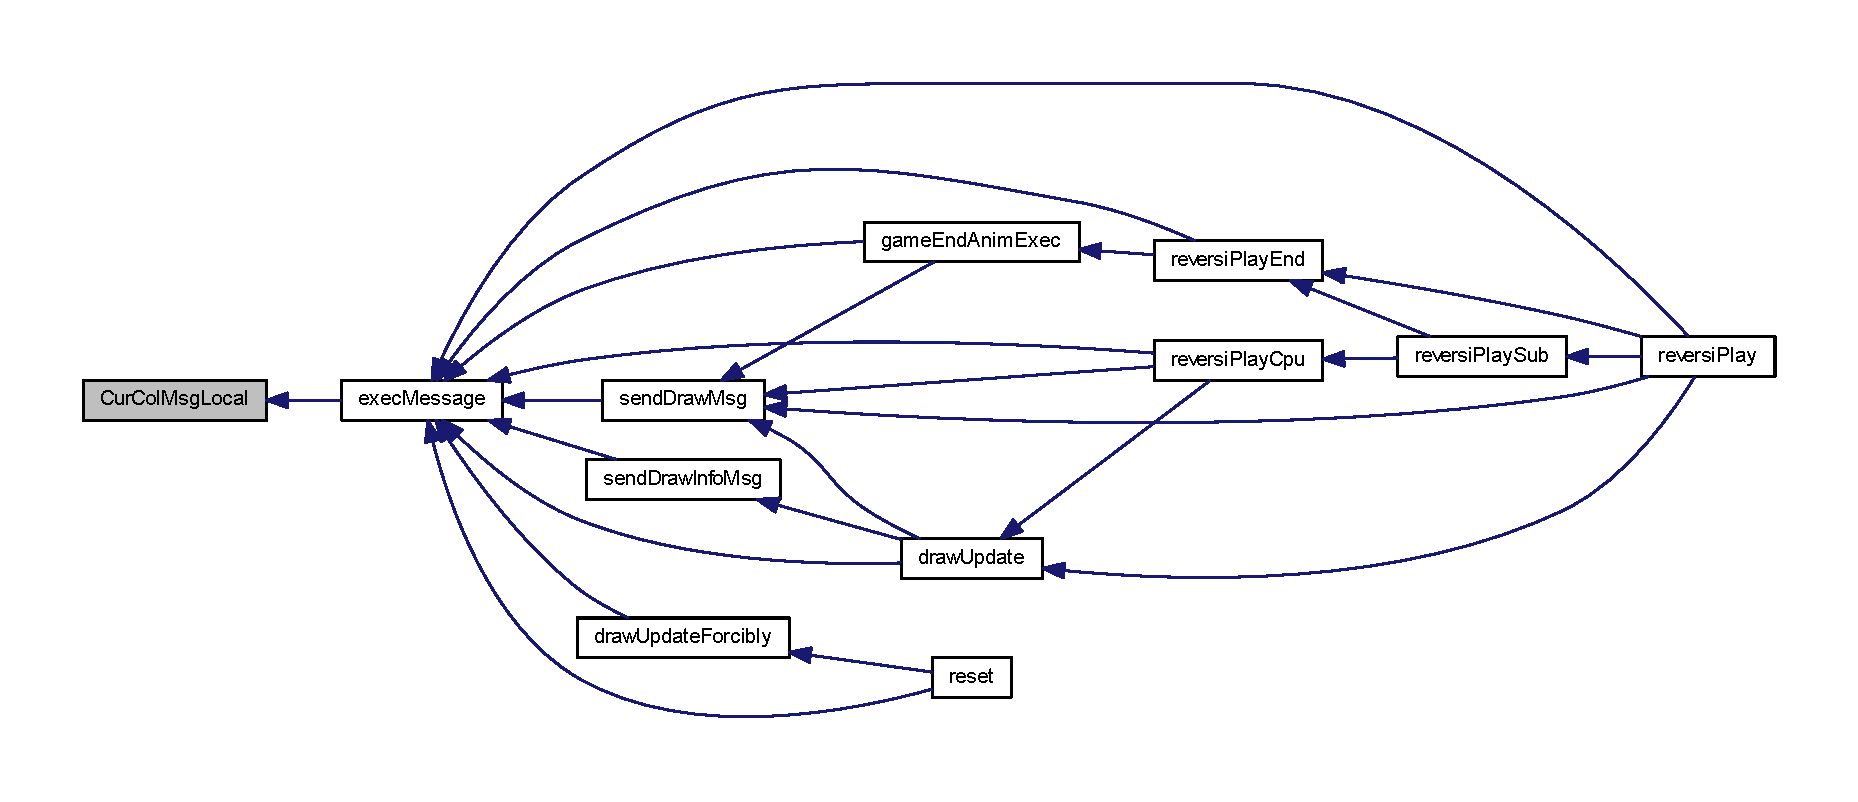
\includegraphics[width=350pt]{class_reversi_play_aa217a221907e90c97719f8332c60a6d6_icgraph}
\end{center}
\end{figure}
\mbox{\Hypertarget{class_reversi_play_ae3da8fb1a3a365c6e5254e5cf6f1e7bc}\label{class_reversi_play_ae3da8fb1a3a365c6e5254e5cf6f1e7bc}} 
\index{Reversi\+Play@{Reversi\+Play}!Cur\+Sts\+Msg\+Local@{Cur\+Sts\+Msg\+Local}}
\index{Cur\+Sts\+Msg\+Local@{Cur\+Sts\+Msg\+Local}!Reversi\+Play@{Reversi\+Play}}
\subsubsection{\texorpdfstring{Cur\+Sts\+Msg\+Local()}{CurStsMsgLocal()}}
{\footnotesize\ttfamily Cur\+Sts\+Msg\+Local (\begin{DoxyParamCaption}\item[{}]{\$text }\end{DoxyParamCaption})\hspace{0.3cm}{\ttfamily [private]}}



現在のステータスメッセージ 


\begin{DoxyParams}[1]{Parameters}
\mbox{\tt in}  & {\em \$text} & テキスト \\
\hline
\end{DoxyParams}
\begin{DoxyReturn}{Returns}
ありません 
\end{DoxyReturn}
\begin{DoxyAuthor}{Author}
Yuta Yoshinaga 
\end{DoxyAuthor}
\begin{DoxyDate}{Date}
2018.\+03.\+02 
\end{DoxyDate}


Definition at line 1125 of file Reversi\+Play.\+php.



Referenced by exec\+Message().

Here is the caller graph for this function\+:
\nopagebreak
\begin{figure}[H]
\begin{center}
\leavevmode
\includegraphics[width=350pt]{class_reversi_play_ae3da8fb1a3a365c6e5254e5cf6f1e7bc_icgraph}
\end{center}
\end{figure}
\mbox{\Hypertarget{class_reversi_play_af0649b9d4a899e0802c739928136de99}\label{class_reversi_play_af0649b9d4a899e0802c739928136de99}} 
\index{Reversi\+Play@{Reversi\+Play}!Draw\+Single\+Local@{Draw\+Single\+Local}}
\index{Draw\+Single\+Local@{Draw\+Single\+Local}!Reversi\+Play@{Reversi\+Play}}
\subsubsection{\texorpdfstring{Draw\+Single\+Local()}{DrawSingleLocal()}}
{\footnotesize\ttfamily Draw\+Single\+Local (\begin{DoxyParamCaption}\item[{}]{\$y,  }\item[{}]{\$x,  }\item[{}]{\$sts,  }\item[{}]{\$bk,  }\item[{}]{\$text }\end{DoxyParamCaption})\hspace{0.3cm}{\ttfamily [private]}}



1マス描画 


\begin{DoxyParams}[1]{Parameters}
\mbox{\tt in}  & {\em \$y} & Y座標 \\
\hline
\mbox{\tt in}  & {\em \$x} & X座標 \\
\hline
\mbox{\tt in}  & {\em \$sts} & ステータス \\
\hline
\mbox{\tt in}  & {\em \$bk} & 背景 \\
\hline
\mbox{\tt in}  & {\em \$text} & テキスト \\
\hline
\end{DoxyParams}
\begin{DoxyReturn}{Returns}
ありません 
\end{DoxyReturn}
\begin{DoxyAuthor}{Author}
Yuta Yoshinaga 
\end{DoxyAuthor}
\begin{DoxyDate}{Date}
2018.\+03.\+02 
\end{DoxyDate}


Definition at line 1091 of file Reversi\+Play.\+php.



Referenced by exec\+Message().

Here is the caller graph for this function\+:
\nopagebreak
\begin{figure}[H]
\begin{center}
\leavevmode
\includegraphics[width=350pt]{class_reversi_play_af0649b9d4a899e0802c739928136de99_icgraph}
\end{center}
\end{figure}
\mbox{\Hypertarget{class_reversi_play_a52029e5f2e049767d1f67c3f5c18ce9f}\label{class_reversi_play_a52029e5f2e049767d1f67c3f5c18ce9f}} 
\index{Reversi\+Play@{Reversi\+Play}!draw\+Update@{draw\+Update}}
\index{draw\+Update@{draw\+Update}!Reversi\+Play@{Reversi\+Play}}
\subsubsection{\texorpdfstring{draw\+Update()}{drawUpdate()}}
{\footnotesize\ttfamily draw\+Update (\begin{DoxyParamCaption}\item[{}]{\$assist }\end{DoxyParamCaption})}



マス描画更新 


\begin{DoxyParams}[1]{Parameters}
\mbox{\tt in}  & {\em \$assist} & アシスト設定 \\
\hline
\end{DoxyParams}
\begin{DoxyReturn}{Returns}
ありません 
\end{DoxyReturn}
\begin{DoxyAuthor}{Author}
Yuta Yoshinaga 
\end{DoxyAuthor}
\begin{DoxyDate}{Date}
2018.\+03.\+02 
\end{DoxyDate}


Definition at line 702 of file Reversi\+Play.\+php.



Referenced by reversi\+Play(), and reversi\+Play\+Cpu().

Here is the call graph for this function\+:
\nopagebreak
\begin{figure}[H]
\begin{center}
\leavevmode
\includegraphics[width=350pt]{class_reversi_play_a52029e5f2e049767d1f67c3f5c18ce9f_cgraph}
\end{center}
\end{figure}
Here is the caller graph for this function\+:
\nopagebreak
\begin{figure}[H]
\begin{center}
\leavevmode
\includegraphics[width=350pt]{class_reversi_play_a52029e5f2e049767d1f67c3f5c18ce9f_icgraph}
\end{center}
\end{figure}
\mbox{\Hypertarget{class_reversi_play_a3ae28eb121caf59932218ea7d1fca81d}\label{class_reversi_play_a3ae28eb121caf59932218ea7d1fca81d}} 
\index{Reversi\+Play@{Reversi\+Play}!draw\+Update\+Forcibly@{draw\+Update\+Forcibly}}
\index{draw\+Update\+Forcibly@{draw\+Update\+Forcibly}!Reversi\+Play@{Reversi\+Play}}
\subsubsection{\texorpdfstring{draw\+Update\+Forcibly()}{drawUpdateForcibly()}}
{\footnotesize\ttfamily draw\+Update\+Forcibly (\begin{DoxyParamCaption}\item[{}]{\$assist }\end{DoxyParamCaption})}



マス描画強制更新 


\begin{DoxyParams}[1]{Parameters}
\mbox{\tt in}  & {\em \$assist} & アシスト設定 \\
\hline
\end{DoxyParams}
\begin{DoxyReturn}{Returns}
ありません 
\end{DoxyReturn}
\begin{DoxyAuthor}{Author}
Yuta Yoshinaga 
\end{DoxyAuthor}
\begin{DoxyDate}{Date}
2018.\+03.\+02 
\end{DoxyDate}


Definition at line 735 of file Reversi\+Play.\+php.



Referenced by reset().

Here is the call graph for this function\+:
\nopagebreak
\begin{figure}[H]
\begin{center}
\leavevmode
\includegraphics[width=350pt]{class_reversi_play_a3ae28eb121caf59932218ea7d1fca81d_cgraph}
\end{center}
\end{figure}
Here is the caller graph for this function\+:
\nopagebreak
\begin{figure}[H]
\begin{center}
\leavevmode
\includegraphics[width=256pt]{class_reversi_play_a3ae28eb121caf59932218ea7d1fca81d_icgraph}
\end{center}
\end{figure}
\mbox{\Hypertarget{class_reversi_play_ae8beea2648c1c5cf722364e84a90edf9}\label{class_reversi_play_ae8beea2648c1c5cf722364e84a90edf9}} 
\index{Reversi\+Play@{Reversi\+Play}!exec\+Message@{exec\+Message}}
\index{exec\+Message@{exec\+Message}!Reversi\+Play@{Reversi\+Play}}
\subsubsection{\texorpdfstring{exec\+Message()}{execMessage()}}
{\footnotesize\ttfamily exec\+Message (\begin{DoxyParamCaption}\item[{}]{\$what,  }\item[{}]{\$obj }\end{DoxyParamCaption})\hspace{0.3cm}{\ttfamily [private]}}



メッセージ 


\begin{DoxyParams}[1]{Parameters}
\mbox{\tt in}  & {\em \$what} & \\
\hline
\mbox{\tt in}  & {\em \$obj} & \\
\hline
\end{DoxyParams}
\begin{DoxyReturn}{Returns}
ありません 
\end{DoxyReturn}
\begin{DoxyAuthor}{Author}
Yuta Yoshinaga 
\end{DoxyAuthor}
\begin{DoxyDate}{Date}
2018.\+03.\+02 
\end{DoxyDate}


Definition at line 972 of file Reversi\+Play.\+php.



Referenced by draw\+Update(), draw\+Update\+Forcibly(), game\+End\+Anim\+Exec(), reset(), reversi\+Play(), reversi\+Play\+Cpu(), reversi\+Play\+End(), reversi\+Play\+Sub(), send\+Draw\+Info\+Msg(), and send\+Draw\+Msg().

Here is the call graph for this function\+:
\nopagebreak
\begin{figure}[H]
\begin{center}
\leavevmode
\includegraphics[width=282pt]{class_reversi_play_ae8beea2648c1c5cf722364e84a90edf9_cgraph}
\end{center}
\end{figure}
Here is the caller graph for this function\+:
\nopagebreak
\begin{figure}[H]
\begin{center}
\leavevmode
\includegraphics[width=350pt]{class_reversi_play_ae8beea2648c1c5cf722364e84a90edf9_icgraph}
\end{center}
\end{figure}
\mbox{\Hypertarget{class_reversi_play_acbcd366da8242203ae52fb685fbc929e}\label{class_reversi_play_acbcd366da8242203ae52fb685fbc929e}} 
\index{Reversi\+Play@{Reversi\+Play}!game\+End\+Anim\+Exec@{game\+End\+Anim\+Exec}}
\index{game\+End\+Anim\+Exec@{game\+End\+Anim\+Exec}!Reversi\+Play@{Reversi\+Play}}
\subsubsection{\texorpdfstring{game\+End\+Anim\+Exec()}{gameEndAnimExec()}}
{\footnotesize\ttfamily game\+End\+Anim\+Exec (\begin{DoxyParamCaption}{ }\end{DoxyParamCaption})}



ゲーム終了アニメーション 

\begin{DoxyReturn}{Returns}
ウェイト時間 
\end{DoxyReturn}
\begin{DoxyAuthor}{Author}
Yuta Yoshinaga 
\end{DoxyAuthor}
\begin{DoxyDate}{Date}
2018.\+03.\+02 
\end{DoxyDate}


Definition at line 845 of file Reversi\+Play.\+php.



Referenced by reversi\+Play\+End().

Here is the call graph for this function\+:
\nopagebreak
\begin{figure}[H]
\begin{center}
\leavevmode
\includegraphics[width=350pt]{class_reversi_play_acbcd366da8242203ae52fb685fbc929e_cgraph}
\end{center}
\end{figure}
Here is the caller graph for this function\+:
\nopagebreak
\begin{figure}[H]
\begin{center}
\leavevmode
\includegraphics[width=350pt]{class_reversi_play_acbcd366da8242203ae52fb685fbc929e_icgraph}
\end{center}
\end{figure}
\mbox{\Hypertarget{class_reversi_play_a26fd2d7723695b69cbfde7e16b55b096}\label{class_reversi_play_a26fd2d7723695b69cbfde7e16b55b096}} 
\index{Reversi\+Play@{Reversi\+Play}!get\+Next\+Col@{get\+Next\+Col}}
\index{get\+Next\+Col@{get\+Next\+Col}!Reversi\+Play@{Reversi\+Play}}
\subsubsection{\texorpdfstring{get\+Next\+Col()}{getNextCol()}}
{\footnotesize\ttfamily public function get\+Next\+Col (\begin{DoxyParamCaption}\item[{}]{\$color }\end{DoxyParamCaption})}



次の色取得 


\begin{DoxyParams}[1]{Parameters}
\mbox{\tt in}  & {\em \$color} & 現在の色 \\
\hline
\end{DoxyParams}
\begin{DoxyReturn}{Returns}
次の色 
\end{DoxyReturn}
\begin{DoxyAuthor}{Author}
Yuta Yoshinaga 
\end{DoxyAuthor}
\begin{DoxyDate}{Date}
2018.\+03.\+02 
\end{DoxyDate}


Definition at line 825 of file Reversi\+Play.\+php.



Referenced by reset(), reversi\+Play(), and reversi\+Play\+Sub().

Here is the caller graph for this function\+:
\nopagebreak
\begin{figure}[H]
\begin{center}
\leavevmode
\includegraphics[width=350pt]{class_reversi_play_a26fd2d7723695b69cbfde7e16b55b096_icgraph}
\end{center}
\end{figure}
\mbox{\Hypertarget{class_reversi_play_a4a20559544fdf4dcb457e258dc976cf8}\label{class_reversi_play_a4a20559544fdf4dcb457e258dc976cf8}} 
\index{Reversi\+Play@{Reversi\+Play}!reset@{reset}}
\index{reset@{reset}!Reversi\+Play@{Reversi\+Play}}
\subsubsection{\texorpdfstring{reset()}{reset()}}
{\footnotesize\ttfamily reset (\begin{DoxyParamCaption}{ }\end{DoxyParamCaption})}



リセット処理 

\begin{DoxyReturn}{Returns}
ありません 
\end{DoxyReturn}
\begin{DoxyAuthor}{Author}
Yuta Yoshinaga 
\end{DoxyAuthor}
\begin{DoxyDate}{Date}
2018.\+03.\+02 
\end{DoxyDate}


Definition at line 760 of file Reversi\+Play.\+php.

Here is the call graph for this function\+:
\nopagebreak
\begin{figure}[H]
\begin{center}
\leavevmode
\includegraphics[width=350pt]{class_reversi_play_a4a20559544fdf4dcb457e258dc976cf8_cgraph}
\end{center}
\end{figure}
\mbox{\Hypertarget{class_reversi_play_a017d2d85f7c5c6917f528f30452d72d0}\label{class_reversi_play_a017d2d85f7c5c6917f528f30452d72d0}} 
\index{Reversi\+Play@{Reversi\+Play}!reversi\+Play@{reversi\+Play}}
\index{reversi\+Play@{reversi\+Play}!Reversi\+Play@{Reversi\+Play}}
\subsubsection{\texorpdfstring{reversi\+Play()}{reversiPlay()}}
{\footnotesize\ttfamily reversi\+Play (\begin{DoxyParamCaption}\item[{}]{\$y,  }\item[{}]{\$x }\end{DoxyParamCaption})}



リバーシプレイ 


\begin{DoxyParams}[1]{Parameters}
\mbox{\tt in}  & {\em \$y} & \$y座標 \\
\hline
\mbox{\tt in}  & {\em \$x} & \$x座標 \\
\hline
\end{DoxyParams}
\begin{DoxyReturn}{Returns}
ありません 
\end{DoxyReturn}
\begin{DoxyAuthor}{Author}
Yuta Yoshinaga 
\end{DoxyAuthor}
\begin{DoxyDate}{Date}
2018.\+03.\+02 
\end{DoxyDate}


Definition at line 191 of file Reversi\+Play.\+php.

Here is the call graph for this function\+:
\nopagebreak
\begin{figure}[H]
\begin{center}
\leavevmode
\includegraphics[width=350pt]{class_reversi_play_a017d2d85f7c5c6917f528f30452d72d0_cgraph}
\end{center}
\end{figure}
\mbox{\Hypertarget{class_reversi_play_a6514ad9244af720ee1ec1777c11e80fb}\label{class_reversi_play_a6514ad9244af720ee1ec1777c11e80fb}} 
\index{Reversi\+Play@{Reversi\+Play}!reversi\+Play\+Cpu@{reversi\+Play\+Cpu}}
\index{reversi\+Play\+Cpu@{reversi\+Play\+Cpu}!Reversi\+Play@{Reversi\+Play}}
\subsubsection{\texorpdfstring{reversi\+Play\+Cpu()}{reversiPlayCpu()}}
{\footnotesize\ttfamily reversi\+Play\+Cpu (\begin{DoxyParamCaption}\item[{}]{\$color,  }\item[{}]{\$cpu\+Ena }\end{DoxyParamCaption})}



リバーシプレイコンピューター 


\begin{DoxyParams}[1]{Parameters}
\mbox{\tt in}  & {\em \$color} & C\+P\+U色 \\
\hline
\mbox{\tt in}  & {\em \$cpu\+Ena} & C\+P\+U有効フラグ \\
\hline
\end{DoxyParams}
\begin{DoxyReturn}{Returns}
ありません 
\end{DoxyReturn}
\begin{DoxyAuthor}{Author}
Yuta Yoshinaga 
\end{DoxyAuthor}
\begin{DoxyDate}{Date}
2018.\+03.\+02 
\end{DoxyDate}


Definition at line 422 of file Reversi\+Play.\+php.



Referenced by reversi\+Play\+Sub().

Here is the call graph for this function\+:
\nopagebreak
\begin{figure}[H]
\begin{center}
\leavevmode
\includegraphics[width=350pt]{class_reversi_play_a6514ad9244af720ee1ec1777c11e80fb_cgraph}
\end{center}
\end{figure}
Here is the caller graph for this function\+:
\nopagebreak
\begin{figure}[H]
\begin{center}
\leavevmode
\includegraphics[width=350pt]{class_reversi_play_a6514ad9244af720ee1ec1777c11e80fb_icgraph}
\end{center}
\end{figure}
\mbox{\Hypertarget{class_reversi_play_af55fe6b6f2005c7da80c696ed692783d}\label{class_reversi_play_af55fe6b6f2005c7da80c696ed692783d}} 
\index{Reversi\+Play@{Reversi\+Play}!reversi\+Play\+End@{reversi\+Play\+End}}
\index{reversi\+Play\+End@{reversi\+Play\+End}!Reversi\+Play@{Reversi\+Play}}
\subsubsection{\texorpdfstring{reversi\+Play\+End()}{reversiPlayEnd()}}
{\footnotesize\ttfamily reversi\+Play\+End (\begin{DoxyParamCaption}{ }\end{DoxyParamCaption})}



リバーシプレイ終了 

\begin{DoxyReturn}{Returns}
ありません 
\end{DoxyReturn}
\begin{DoxyAuthor}{Author}
Yuta Yoshinaga 
\end{DoxyAuthor}
\begin{DoxyDate}{Date}
2018.\+03.\+02 
\end{DoxyDate}


Definition at line 330 of file Reversi\+Play.\+php.



Referenced by reversi\+Play(), and reversi\+Play\+Sub().

Here is the call graph for this function\+:
\nopagebreak
\begin{figure}[H]
\begin{center}
\leavevmode
\includegraphics[width=350pt]{class_reversi_play_af55fe6b6f2005c7da80c696ed692783d_cgraph}
\end{center}
\end{figure}
Here is the caller graph for this function\+:
\nopagebreak
\begin{figure}[H]
\begin{center}
\leavevmode
\includegraphics[width=350pt]{class_reversi_play_af55fe6b6f2005c7da80c696ed692783d_icgraph}
\end{center}
\end{figure}
\mbox{\Hypertarget{class_reversi_play_a67816fe65a87e35d8e8cc35d5d269bcb}\label{class_reversi_play_a67816fe65a87e35d8e8cc35d5d269bcb}} 
\index{Reversi\+Play@{Reversi\+Play}!reversi\+Play\+Pass@{reversi\+Play\+Pass}}
\index{reversi\+Play\+Pass@{reversi\+Play\+Pass}!Reversi\+Play@{Reversi\+Play}}
\subsubsection{\texorpdfstring{reversi\+Play\+Pass()}{reversiPlayPass()}}
{\footnotesize\ttfamily reversi\+Play\+Pass (\begin{DoxyParamCaption}\item[{}]{\$color }\end{DoxyParamCaption})}



リバーシプレイパス 


\begin{DoxyParams}[1]{Parameters}
\mbox{\tt in}  & {\em \$color} & パス色 \\
\hline
\end{DoxyParams}
\begin{DoxyReturn}{Returns}
ありません 
\end{DoxyReturn}
\begin{DoxyAuthor}{Author}
Yuta Yoshinaga 
\end{DoxyAuthor}
\begin{DoxyDate}{Date}
2018.\+03.\+02 
\end{DoxyDate}


Definition at line 400 of file Reversi\+Play.\+php.



Referenced by reversi\+Play(), and reversi\+Play\+Sub().

Here is the caller graph for this function\+:
\nopagebreak
\begin{figure}[H]
\begin{center}
\leavevmode
\includegraphics[width=350pt]{class_reversi_play_a67816fe65a87e35d8e8cc35d5d269bcb_icgraph}
\end{center}
\end{figure}
\mbox{\Hypertarget{class_reversi_play_a990fc6e45b7bdf2dab569f087f8b5a62}\label{class_reversi_play_a990fc6e45b7bdf2dab569f087f8b5a62}} 
\index{Reversi\+Play@{Reversi\+Play}!reversi\+Play\+Sub@{reversi\+Play\+Sub}}
\index{reversi\+Play\+Sub@{reversi\+Play\+Sub}!Reversi\+Play@{Reversi\+Play}}
\subsubsection{\texorpdfstring{reversi\+Play\+Sub()}{reversiPlaySub()}}
{\footnotesize\ttfamily reversi\+Play\+Sub (\begin{DoxyParamCaption}\item[{}]{\$cpu\+Ena,  }\item[{}]{\$tmp\+Col }\end{DoxyParamCaption})}



リバーシプレイサブ 


\begin{DoxyParams}[1]{Parameters}
\mbox{\tt in}  & {\em \$cpu\+Ena} & \\
\hline
\mbox{\tt in}  & {\em \$tmp\+Col} & \\
\hline
\end{DoxyParams}
\begin{DoxyReturn}{Returns}
ありません 
\end{DoxyReturn}
\begin{DoxyAuthor}{Author}
Yuta Yoshinaga 
\end{DoxyAuthor}
\begin{DoxyDate}{Date}
2018.\+03.\+02 
\end{DoxyDate}


Definition at line 289 of file Reversi\+Play.\+php.



Referenced by reversi\+Play().

Here is the call graph for this function\+:
\nopagebreak
\begin{figure}[H]
\begin{center}
\leavevmode
\includegraphics[width=350pt]{class_reversi_play_a990fc6e45b7bdf2dab569f087f8b5a62_cgraph}
\end{center}
\end{figure}
Here is the caller graph for this function\+:
\nopagebreak
\begin{figure}[H]
\begin{center}
\leavevmode
\includegraphics[width=261pt]{class_reversi_play_a990fc6e45b7bdf2dab569f087f8b5a62_icgraph}
\end{center}
\end{figure}
\mbox{\Hypertarget{class_reversi_play_a829b61937e857a9f1b5b371be25dbabd}\label{class_reversi_play_a829b61937e857a9f1b5b371be25dbabd}} 
\index{Reversi\+Play@{Reversi\+Play}!send\+Draw\+Info\+Msg@{send\+Draw\+Info\+Msg}}
\index{send\+Draw\+Info\+Msg@{send\+Draw\+Info\+Msg}!Reversi\+Play@{Reversi\+Play}}
\subsubsection{\texorpdfstring{send\+Draw\+Info\+Msg()}{sendDrawInfoMsg()}}
{\footnotesize\ttfamily send\+Draw\+Info\+Msg (\begin{DoxyParamCaption}\item[{}]{\$y,  }\item[{}]{\$x }\end{DoxyParamCaption})}



情報描画メッセージ送信 


\begin{DoxyParams}[1]{Parameters}
\mbox{\tt in}  & {\em \$y} & Y座標 \\
\hline
\mbox{\tt in}  & {\em \$x} & X座標 \\
\hline
\end{DoxyParams}
\begin{DoxyReturn}{Returns}
ありません 
\end{DoxyReturn}
\begin{DoxyDate}{Date}
2018.\+03.\+02 
\end{DoxyDate}


Definition at line 953 of file Reversi\+Play.\+php.



Referenced by draw\+Update().

Here is the call graph for this function\+:
\nopagebreak
\begin{figure}[H]
\begin{center}
\leavevmode
\includegraphics[width=350pt]{class_reversi_play_a829b61937e857a9f1b5b371be25dbabd_cgraph}
\end{center}
\end{figure}
Here is the caller graph for this function\+:
\nopagebreak
\begin{figure}[H]
\begin{center}
\leavevmode
\includegraphics[width=350pt]{class_reversi_play_a829b61937e857a9f1b5b371be25dbabd_icgraph}
\end{center}
\end{figure}
\mbox{\Hypertarget{class_reversi_play_af27aaf13f15a080c006432338a06c481}\label{class_reversi_play_af27aaf13f15a080c006432338a06c481}} 
\index{Reversi\+Play@{Reversi\+Play}!send\+Draw\+Msg@{send\+Draw\+Msg}}
\index{send\+Draw\+Msg@{send\+Draw\+Msg}!Reversi\+Play@{Reversi\+Play}}
\subsubsection{\texorpdfstring{send\+Draw\+Msg()}{sendDrawMsg()}}
{\footnotesize\ttfamily send\+Draw\+Msg (\begin{DoxyParamCaption}\item[{}]{\$y,  }\item[{}]{\$x }\end{DoxyParamCaption})}



描画メッセージ送信 


\begin{DoxyParams}[1]{Parameters}
\mbox{\tt in}  & {\em \$y} & Y座標 \\
\hline
\mbox{\tt in}  & {\em \$x} & X座標 \\
\hline
\end{DoxyParams}
\begin{DoxyReturn}{Returns}
ありません 
\end{DoxyReturn}
\begin{DoxyAuthor}{Author}
Yuta Yoshinaga 
\end{DoxyAuthor}
\begin{DoxyDate}{Date}
2018.\+03.\+02 
\end{DoxyDate}


Definition at line 935 of file Reversi\+Play.\+php.



Referenced by draw\+Update(), game\+End\+Anim\+Exec(), reversi\+Play(), and reversi\+Play\+Cpu().

Here is the call graph for this function\+:
\nopagebreak
\begin{figure}[H]
\begin{center}
\leavevmode
\includegraphics[width=350pt]{class_reversi_play_af27aaf13f15a080c006432338a06c481_cgraph}
\end{center}
\end{figure}
Here is the caller graph for this function\+:
\nopagebreak
\begin{figure}[H]
\begin{center}
\leavevmode
\includegraphics[width=350pt]{class_reversi_play_af27aaf13f15a080c006432338a06c481_icgraph}
\end{center}
\end{figure}
\mbox{\Hypertarget{class_reversi_play_a2212d70313710a13422dd4fcb5da9cde}\label{class_reversi_play_a2212d70313710a13422dd4fcb5da9cde}} 
\index{Reversi\+Play@{Reversi\+Play}!View\+Msg\+Dlg\+Local@{View\+Msg\+Dlg\+Local}}
\index{View\+Msg\+Dlg\+Local@{View\+Msg\+Dlg\+Local}!Reversi\+Play@{Reversi\+Play}}
\subsubsection{\texorpdfstring{View\+Msg\+Dlg\+Local()}{ViewMsgDlgLocal()}}
{\footnotesize\ttfamily View\+Msg\+Dlg\+Local (\begin{DoxyParamCaption}\item[{}]{\$title,  }\item[{}]{\$msg }\end{DoxyParamCaption})\hspace{0.3cm}{\ttfamily [private]}}



メッセージダイアログ 


\begin{DoxyParams}[1]{Parameters}
\mbox{\tt in}  & {\em \$title} & タイトル \\
\hline
\mbox{\tt in}  & {\em \$msg} & メッセージ \\
\hline
\end{DoxyParams}
\begin{DoxyReturn}{Returns}
ありません 
\end{DoxyReturn}
\begin{DoxyAuthor}{Author}
Yuta Yoshinaga 
\end{DoxyAuthor}
\begin{DoxyDate}{Date}
2018.\+03.\+02 
\end{DoxyDate}


Definition at line 1070 of file Reversi\+Play.\+php.



Referenced by reversi\+Play(), and reversi\+Play\+End().

Here is the caller graph for this function\+:
\nopagebreak
\begin{figure}[H]
\begin{center}
\leavevmode
\includegraphics[width=350pt]{class_reversi_play_a2212d70313710a13422dd4fcb5da9cde_icgraph}
\end{center}
\end{figure}
\mbox{\Hypertarget{class_reversi_play_a58884d8de55d9faeac653fcf6d4f48b3}\label{class_reversi_play_a58884d8de55d9faeac653fcf6d4f48b3}} 
\index{Reversi\+Play@{Reversi\+Play}!Wait\+Local@{Wait\+Local}}
\index{Wait\+Local@{Wait\+Local}!Reversi\+Play@{Reversi\+Play}}
\subsubsection{\texorpdfstring{Wait\+Local()}{WaitLocal()}}
{\footnotesize\ttfamily Wait\+Local (\begin{DoxyParamCaption}\item[{}]{\$time }\end{DoxyParamCaption})\hspace{0.3cm}{\ttfamily [private]}}



ウェイト 


\begin{DoxyParams}[1]{Parameters}
\mbox{\tt in}  & {\em \$time} & ウェイト時間(msec) \\
\hline
\end{DoxyParams}
\begin{DoxyReturn}{Returns}
ありません 
\end{DoxyReturn}
\begin{DoxyAuthor}{Author}
Yuta Yoshinaga 
\end{DoxyAuthor}
\begin{DoxyDate}{Date}
2018.\+03.\+02 
\end{DoxyDate}


Definition at line 1142 of file Reversi\+Play.\+php.



Referenced by draw\+Update(), game\+End\+Anim\+Exec(), reversi\+Play(), and reversi\+Play\+End().

Here is the caller graph for this function\+:
\nopagebreak
\begin{figure}[H]
\begin{center}
\leavevmode
\includegraphics[width=350pt]{class_reversi_play_a58884d8de55d9faeac653fcf6d4f48b3_icgraph}
\end{center}
\end{figure}


The documentation for this class was generated from the following file\+:\begin{DoxyCompactItemize}
\item 
Model/\hyperlink{_reversi_play_8php}{Reversi\+Play.\+php}\end{DoxyCompactItemize}

\hypertarget{class_reversi_point}{}\section{Reversi\+Point Class Reference}
\label{class_reversi_point}\index{Reversi\+Point@{Reversi\+Point}}


リバーシポイント  




Collaboration diagram for Reversi\+Point\+:\nopagebreak
\begin{figure}[H]
\begin{center}
\leavevmode
\includegraphics[width=163pt]{class_reversi_point__coll__graph}
\end{center}
\end{figure}
\subsection*{Public Member Functions}
\begin{DoxyCompactItemize}
\item 
\mbox{\Hypertarget{class_reversi_point_a3088fbd713750a579d57f35c4372c9e0}\label{class_reversi_point_a3088fbd713750a579d57f35c4372c9e0}} 
{\bfseries getx} ()
\item 
\mbox{\Hypertarget{class_reversi_point_a28b8a91d77413e6d64138b9b4c75f365}\label{class_reversi_point_a28b8a91d77413e6d64138b9b4c75f365}} 
{\bfseries setx} (\$\+\_\+x)
\item 
\mbox{\Hypertarget{class_reversi_point_a537d0279caa8c09e7923ca93388c0371}\label{class_reversi_point_a537d0279caa8c09e7923ca93388c0371}} 
{\bfseries gety} ()
\item 
\mbox{\Hypertarget{class_reversi_point_a2d6987f9f9cb43c74fabe08c6117ba9e}\label{class_reversi_point_a2d6987f9f9cb43c74fabe08c6117ba9e}} 
{\bfseries sety} (\$\+\_\+y)
\item 
\hyperlink{class_reversi_point_a095c5d389db211932136b53f25f39685}{\+\_\+\+\_\+construct} ()
\begin{DoxyCompactList}\small\item\em コンストラクタ \end{DoxyCompactList}\item 
\hyperlink{class_reversi_point_a421831a265621325e1fdd19aace0c758}{\+\_\+\+\_\+destruct} ()
\begin{DoxyCompactList}\small\item\em デストラクタ \end{DoxyCompactList}\end{DoxyCompactItemize}
\subsection*{Private Attributes}
\begin{DoxyCompactItemize}
\item 
\mbox{\Hypertarget{class_reversi_point_ae57ae417aad3990d032c704748364c74}\label{class_reversi_point_ae57ae417aad3990d032c704748364c74}} 
\hyperlink{class_reversi_point_ae57ae417aad3990d032c704748364c74}{\$\+\_\+x}
\begin{DoxyCompactList}\small\item\em X. \end{DoxyCompactList}\item 
\mbox{\Hypertarget{class_reversi_point_a44b74e71d07c6bff218f62d98547a399}\label{class_reversi_point_a44b74e71d07c6bff218f62d98547a399}} 
\hyperlink{class_reversi_point_a44b74e71d07c6bff218f62d98547a399}{\$\+\_\+y}
\begin{DoxyCompactList}\small\item\em Y. \end{DoxyCompactList}\end{DoxyCompactItemize}


\subsection{Detailed Description}
リバーシポイント 

Definition at line 25 of file Reversi\+Point.\+php.



\subsection{Constructor \& Destructor Documentation}
\mbox{\Hypertarget{class_reversi_point_a095c5d389db211932136b53f25f39685}\label{class_reversi_point_a095c5d389db211932136b53f25f39685}} 
\index{Reversi\+Point@{Reversi\+Point}!\+\_\+\+\_\+construct@{\+\_\+\+\_\+construct}}
\index{\+\_\+\+\_\+construct@{\+\_\+\+\_\+construct}!Reversi\+Point@{Reversi\+Point}}
\subsubsection{\texorpdfstring{\+\_\+\+\_\+construct()}{\_\_construct()}}
{\footnotesize\ttfamily \+\_\+\+\_\+construct (\begin{DoxyParamCaption}{ }\end{DoxyParamCaption})}



コンストラクタ 

\begin{DoxyReturn}{Returns}
ありません 
\end{DoxyReturn}
\begin{DoxyAuthor}{Author}
Yuta Yoshinaga 
\end{DoxyAuthor}
\begin{DoxyDate}{Date}
2018.\+03.\+02 
\end{DoxyDate}


Definition at line 48 of file Reversi\+Point.\+php.

\mbox{\Hypertarget{class_reversi_point_a421831a265621325e1fdd19aace0c758}\label{class_reversi_point_a421831a265621325e1fdd19aace0c758}} 
\index{Reversi\+Point@{Reversi\+Point}!\+\_\+\+\_\+destruct@{\+\_\+\+\_\+destruct}}
\index{\+\_\+\+\_\+destruct@{\+\_\+\+\_\+destruct}!Reversi\+Point@{Reversi\+Point}}
\subsubsection{\texorpdfstring{\+\_\+\+\_\+destruct()}{\_\_destruct()}}
{\footnotesize\ttfamily \+\_\+\+\_\+destruct (\begin{DoxyParamCaption}{ }\end{DoxyParamCaption})}



デストラクタ 

\begin{DoxyReturn}{Returns}
ありません 
\end{DoxyReturn}
\begin{DoxyAuthor}{Author}
Yuta Yoshinaga 
\end{DoxyAuthor}
\begin{DoxyDate}{Date}
2018.\+03.\+02 
\end{DoxyDate}


Definition at line 62 of file Reversi\+Point.\+php.



The documentation for this class was generated from the following file\+:\begin{DoxyCompactItemize}
\item 
Model/\hyperlink{_reversi_point_8php}{Reversi\+Point.\+php}\end{DoxyCompactItemize}

\hypertarget{class_reversi_setting}{}\section{Reversi\+Setting Class Reference}
\label{class_reversi_setting}\index{Reversi\+Setting@{Reversi\+Setting}}


アプリ設定クラス  




Collaboration diagram for Reversi\+Setting\+:
\nopagebreak
\begin{figure}[H]
\begin{center}
\leavevmode
\includegraphics[width=196pt]{class_reversi_setting__coll__graph}
\end{center}
\end{figure}
\subsection*{Public Member Functions}
\begin{DoxyCompactItemize}
\item 
\mbox{\Hypertarget{class_reversi_setting_a4ed7f3bdbf5c81ccb1d7a110b784d729}\label{class_reversi_setting_a4ed7f3bdbf5c81ccb1d7a110b784d729}} 
{\bfseries getm\+Mode} ()
\item 
\mbox{\Hypertarget{class_reversi_setting_a39167d7120c0f7be3d71fb8b36d4b2d2}\label{class_reversi_setting_a39167d7120c0f7be3d71fb8b36d4b2d2}} 
{\bfseries setm\+Mode} (\$\+\_\+m\+Mode)
\item 
\mbox{\Hypertarget{class_reversi_setting_a4a6f8c370ba7f56090a4589dd764985c}\label{class_reversi_setting_a4a6f8c370ba7f56090a4589dd764985c}} 
{\bfseries getm\+Type} ()
\item 
\mbox{\Hypertarget{class_reversi_setting_ad32dae55a2718993d5b0cf9e85a9a201}\label{class_reversi_setting_ad32dae55a2718993d5b0cf9e85a9a201}} 
{\bfseries setm\+Type} (\$\+\_\+m\+Type)
\item 
\mbox{\Hypertarget{class_reversi_setting_a5070a9ab795fa2f316723066dd9ee7ca}\label{class_reversi_setting_a5070a9ab795fa2f316723066dd9ee7ca}} 
{\bfseries getm\+Player} ()
\item 
\mbox{\Hypertarget{class_reversi_setting_a31f291d8896090ba483ce66a62268843}\label{class_reversi_setting_a31f291d8896090ba483ce66a62268843}} 
{\bfseries setm\+Player} (\$\+\_\+m\+Player)
\item 
\mbox{\Hypertarget{class_reversi_setting_addf31d3fffb8c3d095e7be3fc29e72e6}\label{class_reversi_setting_addf31d3fffb8c3d095e7be3fc29e72e6}} 
{\bfseries getm\+Assist} ()
\item 
\mbox{\Hypertarget{class_reversi_setting_a828afe27a985d264802d155f22cc69c1}\label{class_reversi_setting_a828afe27a985d264802d155f22cc69c1}} 
{\bfseries setm\+Assist} (\$\+\_\+m\+Assist)
\item 
\mbox{\Hypertarget{class_reversi_setting_aa68659744b5089035ba6e945e4d566c8}\label{class_reversi_setting_aa68659744b5089035ba6e945e4d566c8}} 
{\bfseries getm\+Game\+Spd} ()
\item 
\mbox{\Hypertarget{class_reversi_setting_afdb2caa1a2e59f8c25d27c8d4eba2055}\label{class_reversi_setting_afdb2caa1a2e59f8c25d27c8d4eba2055}} 
{\bfseries setm\+Game\+Spd} (\$\+\_\+m\+Game\+Spd)
\item 
\mbox{\Hypertarget{class_reversi_setting_a9c96042c1a1c482e4083d5aff613974a}\label{class_reversi_setting_a9c96042c1a1c482e4083d5aff613974a}} 
{\bfseries getm\+End\+Anim} ()
\item 
\mbox{\Hypertarget{class_reversi_setting_aa999b168a52630ff1e339e8131589f36}\label{class_reversi_setting_aa999b168a52630ff1e339e8131589f36}} 
{\bfseries setm\+End\+Anim} (\$\+\_\+m\+End\+Anim)
\item 
\mbox{\Hypertarget{class_reversi_setting_a7c7134b5c9b4920861676c8aa65fc8bf}\label{class_reversi_setting_a7c7134b5c9b4920861676c8aa65fc8bf}} 
{\bfseries getm\+Masu\+Cnt\+Menu} ()
\item 
\mbox{\Hypertarget{class_reversi_setting_a124deeade23c86db5106d01abd2816d3}\label{class_reversi_setting_a124deeade23c86db5106d01abd2816d3}} 
{\bfseries setm\+Masu\+Cnt\+Menu} (\$\+\_\+m\+Masu\+Cnt\+Menu)
\item 
\mbox{\Hypertarget{class_reversi_setting_a32cebf699f9aa19d9053c143c3562d3a}\label{class_reversi_setting_a32cebf699f9aa19d9053c143c3562d3a}} 
{\bfseries getm\+Masu\+Cnt} ()
\item 
\mbox{\Hypertarget{class_reversi_setting_ad50e5fa90e6a2f53bf71ed04bed603ae}\label{class_reversi_setting_ad50e5fa90e6a2f53bf71ed04bed603ae}} 
{\bfseries setm\+Masu\+Cnt} (\$\+\_\+m\+Masu\+Cnt)
\item 
\mbox{\Hypertarget{class_reversi_setting_a396427325eccd710236622c2122aef39}\label{class_reversi_setting_a396427325eccd710236622c2122aef39}} 
{\bfseries getm\+Play\+Cpu\+Inter\+Val} ()
\item 
\mbox{\Hypertarget{class_reversi_setting_a7e66c7132df49665538ba0e474f84134}\label{class_reversi_setting_a7e66c7132df49665538ba0e474f84134}} 
{\bfseries setm\+Play\+Cpu\+Inter\+Val} (\$\+\_\+m\+Play\+Cpu\+Inter\+Val)
\item 
\mbox{\Hypertarget{class_reversi_setting_a2348e916349e5ff56f02981f5b828c64}\label{class_reversi_setting_a2348e916349e5ff56f02981f5b828c64}} 
{\bfseries getm\+Play\+Draw\+Inter\+Val} ()
\item 
\mbox{\Hypertarget{class_reversi_setting_aa75e022ea7334a71d2c05a5595636d33}\label{class_reversi_setting_aa75e022ea7334a71d2c05a5595636d33}} 
{\bfseries setm\+Play\+Draw\+Inter\+Val} (\$\+\_\+m\+Play\+Draw\+Inter\+Val)
\item 
\mbox{\Hypertarget{class_reversi_setting_a33a44adbf2f49b190bb2b5f51c1c1360}\label{class_reversi_setting_a33a44adbf2f49b190bb2b5f51c1c1360}} 
{\bfseries getm\+End\+Draw\+Inter\+Val} ()
\item 
\mbox{\Hypertarget{class_reversi_setting_a27a5659dfe111d6cad5d9ec19e2254fb}\label{class_reversi_setting_a27a5659dfe111d6cad5d9ec19e2254fb}} 
{\bfseries setm\+End\+Draw\+Inter\+Val} (\$\+\_\+m\+End\+Draw\+Inter\+Val)
\item 
\mbox{\Hypertarget{class_reversi_setting_ae9a3d550ba5709f511fcdc3967684816}\label{class_reversi_setting_ae9a3d550ba5709f511fcdc3967684816}} 
{\bfseries getm\+End\+Inter\+Val} ()
\item 
\mbox{\Hypertarget{class_reversi_setting_aa1c85566dde92e56e7b81f2835d0d89e}\label{class_reversi_setting_aa1c85566dde92e56e7b81f2835d0d89e}} 
{\bfseries setm\+End\+Inter\+Val} (\$\+\_\+m\+End\+Inter\+Val)
\item 
\mbox{\Hypertarget{class_reversi_setting_a4b459d4e6476f142840db591e6d61868}\label{class_reversi_setting_a4b459d4e6476f142840db591e6d61868}} 
{\bfseries getm\+Theme} ()
\item 
\mbox{\Hypertarget{class_reversi_setting_a465e8f25ffb52a084c29e71768b6a0a1}\label{class_reversi_setting_a465e8f25ffb52a084c29e71768b6a0a1}} 
{\bfseries setm\+Theme} (\$\+\_\+m\+Theme)
\item 
\mbox{\Hypertarget{class_reversi_setting_a091d9cd436e68f4c08d26f61fab3a016}\label{class_reversi_setting_a091d9cd436e68f4c08d26f61fab3a016}} 
{\bfseries getm\+Player\+Color1} ()
\item 
\mbox{\Hypertarget{class_reversi_setting_a411006ea8845a27f5e33b4a555254d2d}\label{class_reversi_setting_a411006ea8845a27f5e33b4a555254d2d}} 
{\bfseries setm\+Player\+Color1} (\$\+\_\+m\+Player\+Color1)
\item 
\mbox{\Hypertarget{class_reversi_setting_ad60404de7ef938cb3c26804c07abe7f7}\label{class_reversi_setting_ad60404de7ef938cb3c26804c07abe7f7}} 
{\bfseries getm\+Player\+Color2} ()
\item 
\mbox{\Hypertarget{class_reversi_setting_a0a0e0d287c262fcc7f2fb27e0d9dbf3a}\label{class_reversi_setting_a0a0e0d287c262fcc7f2fb27e0d9dbf3a}} 
{\bfseries setm\+Player\+Color2} (\$\+\_\+m\+Player\+Color2)
\item 
\mbox{\Hypertarget{class_reversi_setting_a540a19fc7d4fb7c17efa3c76403f4061}\label{class_reversi_setting_a540a19fc7d4fb7c17efa3c76403f4061}} 
{\bfseries getm\+Back\+Ground\+Color} ()
\item 
\mbox{\Hypertarget{class_reversi_setting_ae9013ece88de1d06960aeeafe29b27e7}\label{class_reversi_setting_ae9013ece88de1d06960aeeafe29b27e7}} 
{\bfseries setm\+Back\+Ground\+Color} (\$\+\_\+m\+Back\+Ground\+Color)
\item 
\mbox{\Hypertarget{class_reversi_setting_a91454a61fd72638be2703907a8f81a75}\label{class_reversi_setting_a91454a61fd72638be2703907a8f81a75}} 
{\bfseries getm\+Border\+Color} ()
\item 
\mbox{\Hypertarget{class_reversi_setting_a59c73e106597e9e52ad6f531f7de2ffd}\label{class_reversi_setting_a59c73e106597e9e52ad6f531f7de2ffd}} 
{\bfseries setm\+Border\+Color} (\$\+\_\+m\+Border\+Color)
\item 
\hyperlink{class_reversi_setting_a095c5d389db211932136b53f25f39685}{\+\_\+\+\_\+construct} ()
\begin{DoxyCompactList}\small\item\em コンストラクタ \end{DoxyCompactList}\item 
\hyperlink{class_reversi_setting_a421831a265621325e1fdd19aace0c758}{\+\_\+\+\_\+destruct} ()
\begin{DoxyCompactList}\small\item\em デストラクタ \end{DoxyCompactList}\item 
\hyperlink{class_reversi_setting_a4a20559544fdf4dcb457e258dc976cf8}{reset} ()
\begin{DoxyCompactList}\small\item\em リセット \end{DoxyCompactList}\end{DoxyCompactItemize}
\subsection*{Private Attributes}
\begin{DoxyCompactItemize}
\item 
\mbox{\Hypertarget{class_reversi_setting_ab2c22d6906c36abfd54afdfa293c60d3}\label{class_reversi_setting_ab2c22d6906c36abfd54afdfa293c60d3}} 
\hyperlink{class_reversi_setting_ab2c22d6906c36abfd54afdfa293c60d3}{\$\+\_\+m\+Mode}
\begin{DoxyCompactList}\small\item\em 現在のモード \end{DoxyCompactList}\item 
\mbox{\Hypertarget{class_reversi_setting_ad08340b850f9df7dbdac88cfa433540b}\label{class_reversi_setting_ad08340b850f9df7dbdac88cfa433540b}} 
\hyperlink{class_reversi_setting_ad08340b850f9df7dbdac88cfa433540b}{\$\+\_\+m\+Type}
\begin{DoxyCompactList}\small\item\em 現在のタイプ \end{DoxyCompactList}\item 
\mbox{\Hypertarget{class_reversi_setting_a0e894bb84d15c54a99b589bed9810219}\label{class_reversi_setting_a0e894bb84d15c54a99b589bed9810219}} 
\hyperlink{class_reversi_setting_a0e894bb84d15c54a99b589bed9810219}{\$\+\_\+m\+Player}
\begin{DoxyCompactList}\small\item\em プレイヤーの色 \end{DoxyCompactList}\item 
\mbox{\Hypertarget{class_reversi_setting_abbf625c7eb110bcefecf118d8ee7f10b}\label{class_reversi_setting_abbf625c7eb110bcefecf118d8ee7f10b}} 
\hyperlink{class_reversi_setting_abbf625c7eb110bcefecf118d8ee7f10b}{\$\+\_\+m\+Assist}
\begin{DoxyCompactList}\small\item\em アシスト \end{DoxyCompactList}\item 
\mbox{\Hypertarget{class_reversi_setting_ab9e6faf17330cd3e036bb0fc4274ba57}\label{class_reversi_setting_ab9e6faf17330cd3e036bb0fc4274ba57}} 
\hyperlink{class_reversi_setting_ab9e6faf17330cd3e036bb0fc4274ba57}{\$\+\_\+m\+Game\+Spd}
\begin{DoxyCompactList}\small\item\em ゲームスピード \end{DoxyCompactList}\item 
\mbox{\Hypertarget{class_reversi_setting_a1e4eac5673a529e6e630afe1c889319c}\label{class_reversi_setting_a1e4eac5673a529e6e630afe1c889319c}} 
\hyperlink{class_reversi_setting_a1e4eac5673a529e6e630afe1c889319c}{\$\+\_\+m\+End\+Anim}
\begin{DoxyCompactList}\small\item\em ゲーム終了アニメーション \end{DoxyCompactList}\item 
\mbox{\Hypertarget{class_reversi_setting_a256b36de7f0fcb8aea394a94ae391e87}\label{class_reversi_setting_a256b36de7f0fcb8aea394a94ae391e87}} 
\hyperlink{class_reversi_setting_a256b36de7f0fcb8aea394a94ae391e87}{\$\+\_\+m\+Masu\+Cnt\+Menu}
\begin{DoxyCompactList}\small\item\em マスの数 \end{DoxyCompactList}\item 
\mbox{\Hypertarget{class_reversi_setting_a8ac63bcef31cc4d29b244456c62677bc}\label{class_reversi_setting_a8ac63bcef31cc4d29b244456c62677bc}} 
\hyperlink{class_reversi_setting_a8ac63bcef31cc4d29b244456c62677bc}{\$\+\_\+m\+Masu\+Cnt}
\begin{DoxyCompactList}\small\item\em マスの数 \end{DoxyCompactList}\item 
\mbox{\Hypertarget{class_reversi_setting_abbab445bf7521e93473d7061ee4a5d45}\label{class_reversi_setting_abbab445bf7521e93473d7061ee4a5d45}} 
\hyperlink{class_reversi_setting_abbab445bf7521e93473d7061ee4a5d45}{\$\+\_\+m\+Play\+Cpu\+Inter\+Val}
\begin{DoxyCompactList}\small\item\em C\+P\+U対戦時のインターバル(msec) \end{DoxyCompactList}\item 
\mbox{\Hypertarget{class_reversi_setting_aaea35d8066ead659c17e692292d6c1a4}\label{class_reversi_setting_aaea35d8066ead659c17e692292d6c1a4}} 
\hyperlink{class_reversi_setting_aaea35d8066ead659c17e692292d6c1a4}{\$\+\_\+m\+Play\+Draw\+Inter\+Val}
\begin{DoxyCompactList}\small\item\em 描画のインターバル(msec) \end{DoxyCompactList}\item 
\mbox{\Hypertarget{class_reversi_setting_a21db3633a045483d7b1f2ad85b71ebbb}\label{class_reversi_setting_a21db3633a045483d7b1f2ad85b71ebbb}} 
\hyperlink{class_reversi_setting_a21db3633a045483d7b1f2ad85b71ebbb}{\$\+\_\+m\+End\+Draw\+Inter\+Val}
\begin{DoxyCompactList}\small\item\em 終了アニメーション描画のインターバル(msec) \end{DoxyCompactList}\item 
\mbox{\Hypertarget{class_reversi_setting_a9a7c91b280df7302a2545e8249f7a98b}\label{class_reversi_setting_a9a7c91b280df7302a2545e8249f7a98b}} 
\hyperlink{class_reversi_setting_a9a7c91b280df7302a2545e8249f7a98b}{\$\+\_\+m\+End\+Inter\+Val}
\begin{DoxyCompactList}\small\item\em 終了アニメーションのインターバル(msec) \end{DoxyCompactList}\item 
\mbox{\Hypertarget{class_reversi_setting_a473e416a1757c023d7bd59a5ea12b12a}\label{class_reversi_setting_a473e416a1757c023d7bd59a5ea12b12a}} 
\hyperlink{class_reversi_setting_a473e416a1757c023d7bd59a5ea12b12a}{\$\+\_\+m\+Theme}
\begin{DoxyCompactList}\small\item\em テーマ \end{DoxyCompactList}\item 
\mbox{\Hypertarget{class_reversi_setting_a8e0bf25cff29a3743b30c7a6d17a4855}\label{class_reversi_setting_a8e0bf25cff29a3743b30c7a6d17a4855}} 
\hyperlink{class_reversi_setting_a8e0bf25cff29a3743b30c7a6d17a4855}{\$\+\_\+m\+Player\+Color1}
\begin{DoxyCompactList}\small\item\em プレイヤー1の色 \end{DoxyCompactList}\item 
\mbox{\Hypertarget{class_reversi_setting_a15cb29ead1e4f1bb90eb82819317ea87}\label{class_reversi_setting_a15cb29ead1e4f1bb90eb82819317ea87}} 
\hyperlink{class_reversi_setting_a15cb29ead1e4f1bb90eb82819317ea87}{\$\+\_\+m\+Player\+Color2}
\begin{DoxyCompactList}\small\item\em プレイヤー2の色 \end{DoxyCompactList}\item 
\mbox{\Hypertarget{class_reversi_setting_a69c86bb449573ccc89975e29066e71d7}\label{class_reversi_setting_a69c86bb449573ccc89975e29066e71d7}} 
\hyperlink{class_reversi_setting_a69c86bb449573ccc89975e29066e71d7}{\$\+\_\+m\+Back\+Ground\+Color}
\begin{DoxyCompactList}\small\item\em 背景の色 \end{DoxyCompactList}\item 
\mbox{\Hypertarget{class_reversi_setting_a901c34066dafa1810c09bc3037e692f6}\label{class_reversi_setting_a901c34066dafa1810c09bc3037e692f6}} 
\hyperlink{class_reversi_setting_a901c34066dafa1810c09bc3037e692f6}{\$\+\_\+m\+Border\+Color}
\begin{DoxyCompactList}\small\item\em 枠線の色 \end{DoxyCompactList}\end{DoxyCompactItemize}


\subsection{Detailed Description}
アプリ設定クラス 

Definition at line 27 of file Reversi\+Setting.\+php.



\subsection{Constructor \& Destructor Documentation}
\mbox{\Hypertarget{class_reversi_setting_a095c5d389db211932136b53f25f39685}\label{class_reversi_setting_a095c5d389db211932136b53f25f39685}} 
\index{Reversi\+Setting@{Reversi\+Setting}!\+\_\+\+\_\+construct@{\+\_\+\+\_\+construct}}
\index{\+\_\+\+\_\+construct@{\+\_\+\+\_\+construct}!Reversi\+Setting@{Reversi\+Setting}}
\subsubsection{\texorpdfstring{\+\_\+\+\_\+construct()}{\_\_construct()}}
{\footnotesize\ttfamily \+\_\+\+\_\+construct (\begin{DoxyParamCaption}{ }\end{DoxyParamCaption})}



コンストラクタ 

\begin{DoxyReturn}{Returns}
ありません 
\end{DoxyReturn}
\begin{DoxyAuthor}{Author}
Yuta Yoshinaga 
\end{DoxyAuthor}
\begin{DoxyDate}{Date}
2018.\+03.\+02 
\end{DoxyDate}


Definition at line 111 of file Reversi\+Setting.\+php.

Here is the call graph for this function\+:
\nopagebreak
\begin{figure}[H]
\begin{center}
\leavevmode
\includegraphics[width=222pt]{class_reversi_setting_a095c5d389db211932136b53f25f39685_cgraph}
\end{center}
\end{figure}
\mbox{\Hypertarget{class_reversi_setting_a421831a265621325e1fdd19aace0c758}\label{class_reversi_setting_a421831a265621325e1fdd19aace0c758}} 
\index{Reversi\+Setting@{Reversi\+Setting}!\+\_\+\+\_\+destruct@{\+\_\+\+\_\+destruct}}
\index{\+\_\+\+\_\+destruct@{\+\_\+\+\_\+destruct}!Reversi\+Setting@{Reversi\+Setting}}
\subsubsection{\texorpdfstring{\+\_\+\+\_\+destruct()}{\_\_destruct()}}
{\footnotesize\ttfamily \+\_\+\+\_\+destruct (\begin{DoxyParamCaption}{ }\end{DoxyParamCaption})}



デストラクタ 

\begin{DoxyReturn}{Returns}
ありません 
\end{DoxyReturn}
\begin{DoxyAuthor}{Author}
Yuta Yoshinaga 
\end{DoxyAuthor}
\begin{DoxyDate}{Date}
2018.\+03.\+02 
\end{DoxyDate}


Definition at line 124 of file Reversi\+Setting.\+php.



\subsection{Member Function Documentation}
\mbox{\Hypertarget{class_reversi_setting_a4a20559544fdf4dcb457e258dc976cf8}\label{class_reversi_setting_a4a20559544fdf4dcb457e258dc976cf8}} 
\index{Reversi\+Setting@{Reversi\+Setting}!reset@{reset}}
\index{reset@{reset}!Reversi\+Setting@{Reversi\+Setting}}
\subsubsection{\texorpdfstring{reset()}{reset()}}
{\footnotesize\ttfamily reset (\begin{DoxyParamCaption}{ }\end{DoxyParamCaption})}



リセット 

\begin{DoxyReturn}{Returns}
ありません 
\end{DoxyReturn}
\begin{DoxyAuthor}{Author}
Yuta Yoshinaga 
\end{DoxyAuthor}
\begin{DoxyDate}{Date}
2018.\+03.\+02 
\end{DoxyDate}


Definition at line 136 of file Reversi\+Setting.\+php.



Referenced by \+\_\+\+\_\+construct().

Here is the caller graph for this function\+:
\nopagebreak
\begin{figure}[H]
\begin{center}
\leavevmode
\includegraphics[width=222pt]{class_reversi_setting_a4a20559544fdf4dcb457e258dc976cf8_icgraph}
\end{center}
\end{figure}


The documentation for this class was generated from the following file\+:\begin{DoxyCompactItemize}
\item 
Model/\hyperlink{_reversi_setting_8php}{Reversi\+Setting.\+php}\end{DoxyCompactItemize}

\hypertarget{class_test_reversi}{}\section{Test\+Reversi Class Reference}
\label{class_test_reversi}\index{Test\+Reversi@{Test\+Reversi}}


アプリ設定クラステストドライバー  




Collaboration diagram for Test\+Reversi\+:
\nopagebreak
\begin{figure}[H]
\begin{center}
\leavevmode
\includegraphics[width=163pt]{class_test_reversi__coll__graph}
\end{center}
\end{figure}
\subsection*{Public Member Functions}
\begin{DoxyCompactItemize}
\item 
\hyperlink{class_test_reversi_a095c5d389db211932136b53f25f39685}{\+\_\+\+\_\+construct} ()
\begin{DoxyCompactList}\small\item\em コンストラクタ \end{DoxyCompactList}\item 
\hyperlink{class_test_reversi_a421831a265621325e1fdd19aace0c758}{\+\_\+\+\_\+destruct} ()
\begin{DoxyCompactList}\small\item\em デストラクタ \end{DoxyCompactList}\item 
\hyperlink{class_test_reversi_a9b029832cfdf19c0ef36b1f5ef7b7735}{test\+\_\+run} ()
\begin{DoxyCompactList}\small\item\em テスト実行 \end{DoxyCompactList}\end{DoxyCompactItemize}


\subsection{Detailed Description}
アプリ設定クラステストドライバー 

Definition at line 27 of file Test\+Reversi.\+php.



\subsection{Constructor \& Destructor Documentation}
\mbox{\Hypertarget{class_test_reversi_a095c5d389db211932136b53f25f39685}\label{class_test_reversi_a095c5d389db211932136b53f25f39685}} 
\index{Test\+Reversi@{Test\+Reversi}!\+\_\+\+\_\+construct@{\+\_\+\+\_\+construct}}
\index{\+\_\+\+\_\+construct@{\+\_\+\+\_\+construct}!Test\+Reversi@{Test\+Reversi}}
\subsubsection{\texorpdfstring{\+\_\+\+\_\+construct()}{\_\_construct()}}
{\footnotesize\ttfamily \+\_\+\+\_\+construct (\begin{DoxyParamCaption}{ }\end{DoxyParamCaption})}



コンストラクタ 

\begin{DoxyReturn}{Returns}
ありません 
\end{DoxyReturn}
\begin{DoxyAuthor}{Author}
Yuta Yoshinaga 
\end{DoxyAuthor}
\begin{DoxyDate}{Date}
2018.\+03.\+02 
\end{DoxyDate}


Definition at line 37 of file Test\+Reversi.\+php.

\mbox{\Hypertarget{class_test_reversi_a421831a265621325e1fdd19aace0c758}\label{class_test_reversi_a421831a265621325e1fdd19aace0c758}} 
\index{Test\+Reversi@{Test\+Reversi}!\+\_\+\+\_\+destruct@{\+\_\+\+\_\+destruct}}
\index{\+\_\+\+\_\+destruct@{\+\_\+\+\_\+destruct}!Test\+Reversi@{Test\+Reversi}}
\subsubsection{\texorpdfstring{\+\_\+\+\_\+destruct()}{\_\_destruct()}}
{\footnotesize\ttfamily \+\_\+\+\_\+destruct (\begin{DoxyParamCaption}{ }\end{DoxyParamCaption})}



デストラクタ 

\begin{DoxyReturn}{Returns}
ありません 
\end{DoxyReturn}
\begin{DoxyAuthor}{Author}
Yuta Yoshinaga 
\end{DoxyAuthor}
\begin{DoxyDate}{Date}
2018.\+03.\+02 
\end{DoxyDate}


Definition at line 49 of file Test\+Reversi.\+php.



\subsection{Member Function Documentation}
\mbox{\Hypertarget{class_test_reversi_a9b029832cfdf19c0ef36b1f5ef7b7735}\label{class_test_reversi_a9b029832cfdf19c0ef36b1f5ef7b7735}} 
\index{Test\+Reversi@{Test\+Reversi}!test\+\_\+run@{test\+\_\+run}}
\index{test\+\_\+run@{test\+\_\+run}!Test\+Reversi@{Test\+Reversi}}
\subsubsection{\texorpdfstring{test\+\_\+run()}{test\_run()}}
{\footnotesize\ttfamily test\+\_\+run (\begin{DoxyParamCaption}{ }\end{DoxyParamCaption})}



テスト実行 

\begin{DoxyReturn}{Returns}
ありません 
\end{DoxyReturn}
\begin{DoxyAuthor}{Author}
Yuta Yoshinaga 
\end{DoxyAuthor}
\begin{DoxyDate}{Date}
2018.\+03.\+02 
\end{DoxyDate}


Definition at line 61 of file Test\+Reversi.\+php.



The documentation for this class was generated from the following file\+:\begin{DoxyCompactItemize}
\item 
Test/\hyperlink{_test_reversi_8php}{Test\+Reversi.\+php}\end{DoxyCompactItemize}

\hypertarget{class_test_reversi_anz}{}\section{Test\+Reversi\+Anz Class Reference}
\label{class_test_reversi_anz}\index{Test\+Reversi\+Anz@{Test\+Reversi\+Anz}}


リバーシ解析クラステストドライバー  




Collaboration diagram for Test\+Reversi\+Anz\+:\nopagebreak
\begin{figure}[H]
\begin{center}
\leavevmode
\includegraphics[width=164pt]{class_test_reversi_anz__coll__graph}
\end{center}
\end{figure}
\subsection*{Public Member Functions}
\begin{DoxyCompactItemize}
\item 
\hyperlink{class_test_reversi_anz_a095c5d389db211932136b53f25f39685}{\+\_\+\+\_\+construct} ()
\begin{DoxyCompactList}\small\item\em コンストラクタ \end{DoxyCompactList}\item 
\hyperlink{class_test_reversi_anz_a421831a265621325e1fdd19aace0c758}{\+\_\+\+\_\+destruct} ()
\begin{DoxyCompactList}\small\item\em デストラクタ \end{DoxyCompactList}\item 
\hyperlink{class_test_reversi_anz_a9b029832cfdf19c0ef36b1f5ef7b7735}{test\+\_\+run} ()
\begin{DoxyCompactList}\small\item\em テスト実行 \end{DoxyCompactList}\end{DoxyCompactItemize}


\subsection{Detailed Description}
リバーシ解析クラステストドライバー 

Definition at line 27 of file Test\+Reversi\+Anz.\+php.



\subsection{Constructor \& Destructor Documentation}
\mbox{\Hypertarget{class_test_reversi_anz_a095c5d389db211932136b53f25f39685}\label{class_test_reversi_anz_a095c5d389db211932136b53f25f39685}} 
\index{Test\+Reversi\+Anz@{Test\+Reversi\+Anz}!\+\_\+\+\_\+construct@{\+\_\+\+\_\+construct}}
\index{\+\_\+\+\_\+construct@{\+\_\+\+\_\+construct}!Test\+Reversi\+Anz@{Test\+Reversi\+Anz}}
\subsubsection{\texorpdfstring{\+\_\+\+\_\+construct()}{\_\_construct()}}
{\footnotesize\ttfamily \+\_\+\+\_\+construct (\begin{DoxyParamCaption}{ }\end{DoxyParamCaption})}



コンストラクタ 

\begin{DoxyReturn}{Returns}
ありません 
\end{DoxyReturn}
\begin{DoxyAuthor}{Author}
Yuta Yoshinaga 
\end{DoxyAuthor}
\begin{DoxyDate}{Date}
2018.\+03.\+02 
\end{DoxyDate}


Definition at line 37 of file Test\+Reversi\+Anz.\+php.

\mbox{\Hypertarget{class_test_reversi_anz_a421831a265621325e1fdd19aace0c758}\label{class_test_reversi_anz_a421831a265621325e1fdd19aace0c758}} 
\index{Test\+Reversi\+Anz@{Test\+Reversi\+Anz}!\+\_\+\+\_\+destruct@{\+\_\+\+\_\+destruct}}
\index{\+\_\+\+\_\+destruct@{\+\_\+\+\_\+destruct}!Test\+Reversi\+Anz@{Test\+Reversi\+Anz}}
\subsubsection{\texorpdfstring{\+\_\+\+\_\+destruct()}{\_\_destruct()}}
{\footnotesize\ttfamily \+\_\+\+\_\+destruct (\begin{DoxyParamCaption}{ }\end{DoxyParamCaption})}



デストラクタ 

\begin{DoxyReturn}{Returns}
ありません 
\end{DoxyReturn}
\begin{DoxyAuthor}{Author}
Yuta Yoshinaga 
\end{DoxyAuthor}
\begin{DoxyDate}{Date}
2018.\+03.\+02 
\end{DoxyDate}


Definition at line 49 of file Test\+Reversi\+Anz.\+php.



\subsection{Member Function Documentation}
\mbox{\Hypertarget{class_test_reversi_anz_a9b029832cfdf19c0ef36b1f5ef7b7735}\label{class_test_reversi_anz_a9b029832cfdf19c0ef36b1f5ef7b7735}} 
\index{Test\+Reversi\+Anz@{Test\+Reversi\+Anz}!test\+\_\+run@{test\+\_\+run}}
\index{test\+\_\+run@{test\+\_\+run}!Test\+Reversi\+Anz@{Test\+Reversi\+Anz}}
\subsubsection{\texorpdfstring{test\+\_\+run()}{test\_run()}}
{\footnotesize\ttfamily test\+\_\+run (\begin{DoxyParamCaption}{ }\end{DoxyParamCaption})}



テスト実行 

\begin{DoxyReturn}{Returns}
ありません 
\end{DoxyReturn}
\begin{DoxyAuthor}{Author}
Yuta Yoshinaga 
\end{DoxyAuthor}
\begin{DoxyDate}{Date}
2018.\+03.\+02 
\end{DoxyDate}


Definition at line 61 of file Test\+Reversi\+Anz.\+php.



The documentation for this class was generated from the following file\+:\begin{DoxyCompactItemize}
\item 
Test/\hyperlink{_test_reversi_anz_8php}{Test\+Reversi\+Anz.\+php}\end{DoxyCompactItemize}

\hypertarget{class_test_reversi_history}{}\section{Test\+Reversi\+History Class Reference}
\label{class_test_reversi_history}\index{Test\+Reversi\+History@{Test\+Reversi\+History}}


リバーシ履歴クラステストドライバー  




Collaboration diagram for Test\+Reversi\+History\+:
\nopagebreak
\begin{figure}[H]
\begin{center}
\leavevmode
\includegraphics[width=178pt]{class_test_reversi_history__coll__graph}
\end{center}
\end{figure}
\subsection*{Public Member Functions}
\begin{DoxyCompactItemize}
\item 
\hyperlink{class_test_reversi_history_a095c5d389db211932136b53f25f39685}{\+\_\+\+\_\+construct} ()
\begin{DoxyCompactList}\small\item\em コンストラクタ \end{DoxyCompactList}\item 
\hyperlink{class_test_reversi_history_a421831a265621325e1fdd19aace0c758}{\+\_\+\+\_\+destruct} ()
\begin{DoxyCompactList}\small\item\em デストラクタ \end{DoxyCompactList}\item 
\hyperlink{class_test_reversi_history_a9b029832cfdf19c0ef36b1f5ef7b7735}{test\+\_\+run} ()
\begin{DoxyCompactList}\small\item\em テスト実行 \end{DoxyCompactList}\end{DoxyCompactItemize}


\subsection{Detailed Description}
リバーシ履歴クラステストドライバー 

Definition at line 27 of file Test\+Reversi\+History.\+php.



\subsection{Constructor \& Destructor Documentation}
\mbox{\Hypertarget{class_test_reversi_history_a095c5d389db211932136b53f25f39685}\label{class_test_reversi_history_a095c5d389db211932136b53f25f39685}} 
\index{Test\+Reversi\+History@{Test\+Reversi\+History}!\+\_\+\+\_\+construct@{\+\_\+\+\_\+construct}}
\index{\+\_\+\+\_\+construct@{\+\_\+\+\_\+construct}!Test\+Reversi\+History@{Test\+Reversi\+History}}
\subsubsection{\texorpdfstring{\+\_\+\+\_\+construct()}{\_\_construct()}}
{\footnotesize\ttfamily \+\_\+\+\_\+construct (\begin{DoxyParamCaption}{ }\end{DoxyParamCaption})}



コンストラクタ 

\begin{DoxyReturn}{Returns}
ありません 
\end{DoxyReturn}
\begin{DoxyAuthor}{Author}
Yuta Yoshinaga 
\end{DoxyAuthor}
\begin{DoxyDate}{Date}
2018.\+03.\+02 
\end{DoxyDate}


Definition at line 37 of file Test\+Reversi\+History.\+php.

\mbox{\Hypertarget{class_test_reversi_history_a421831a265621325e1fdd19aace0c758}\label{class_test_reversi_history_a421831a265621325e1fdd19aace0c758}} 
\index{Test\+Reversi\+History@{Test\+Reversi\+History}!\+\_\+\+\_\+destruct@{\+\_\+\+\_\+destruct}}
\index{\+\_\+\+\_\+destruct@{\+\_\+\+\_\+destruct}!Test\+Reversi\+History@{Test\+Reversi\+History}}
\subsubsection{\texorpdfstring{\+\_\+\+\_\+destruct()}{\_\_destruct()}}
{\footnotesize\ttfamily \+\_\+\+\_\+destruct (\begin{DoxyParamCaption}{ }\end{DoxyParamCaption})}



デストラクタ 

\begin{DoxyReturn}{Returns}
ありません 
\end{DoxyReturn}
\begin{DoxyAuthor}{Author}
Yuta Yoshinaga 
\end{DoxyAuthor}
\begin{DoxyDate}{Date}
2018.\+03.\+02 
\end{DoxyDate}


Definition at line 49 of file Test\+Reversi\+History.\+php.



\subsection{Member Function Documentation}
\mbox{\Hypertarget{class_test_reversi_history_a9b029832cfdf19c0ef36b1f5ef7b7735}\label{class_test_reversi_history_a9b029832cfdf19c0ef36b1f5ef7b7735}} 
\index{Test\+Reversi\+History@{Test\+Reversi\+History}!test\+\_\+run@{test\+\_\+run}}
\index{test\+\_\+run@{test\+\_\+run}!Test\+Reversi\+History@{Test\+Reversi\+History}}
\subsubsection{\texorpdfstring{test\+\_\+run()}{test\_run()}}
{\footnotesize\ttfamily test\+\_\+run (\begin{DoxyParamCaption}{ }\end{DoxyParamCaption})}



テスト実行 

\begin{DoxyReturn}{Returns}
ありません 
\end{DoxyReturn}
\begin{DoxyAuthor}{Author}
Yuta Yoshinaga 
\end{DoxyAuthor}
\begin{DoxyDate}{Date}
2018.\+03.\+02 
\end{DoxyDate}


Definition at line 61 of file Test\+Reversi\+History.\+php.



The documentation for this class was generated from the following file\+:\begin{DoxyCompactItemize}
\item 
Test/\hyperlink{_test_reversi_history_8php}{Test\+Reversi\+History.\+php}\end{DoxyCompactItemize}

\hypertarget{class_test_reversi_play}{}\section{Test\+Reversi\+Play Class Reference}
\label{class_test_reversi_play}\index{Test\+Reversi\+Play@{Test\+Reversi\+Play}}


アプリ設定クラステストドライバー  




Collaboration diagram for Test\+Reversi\+Play\+:\nopagebreak
\begin{figure}[H]
\begin{center}
\leavevmode
\includegraphics[width=166pt]{class_test_reversi_play__coll__graph}
\end{center}
\end{figure}
\subsection*{Public Member Functions}
\begin{DoxyCompactItemize}
\item 
\hyperlink{class_test_reversi_play_a095c5d389db211932136b53f25f39685}{\+\_\+\+\_\+construct} ()
\begin{DoxyCompactList}\small\item\em コンストラクタ \end{DoxyCompactList}\item 
\hyperlink{class_test_reversi_play_a421831a265621325e1fdd19aace0c758}{\+\_\+\+\_\+destruct} ()
\begin{DoxyCompactList}\small\item\em デストラクタ \end{DoxyCompactList}\item 
\hyperlink{class_test_reversi_play_a9b029832cfdf19c0ef36b1f5ef7b7735}{test\+\_\+run} ()
\begin{DoxyCompactList}\small\item\em テスト実行 \end{DoxyCompactList}\end{DoxyCompactItemize}


\subsection{Detailed Description}
アプリ設定クラステストドライバー 

Definition at line 27 of file Test\+Reversi\+Play.\+php.



\subsection{Constructor \& Destructor Documentation}
\mbox{\Hypertarget{class_test_reversi_play_a095c5d389db211932136b53f25f39685}\label{class_test_reversi_play_a095c5d389db211932136b53f25f39685}} 
\index{Test\+Reversi\+Play@{Test\+Reversi\+Play}!\+\_\+\+\_\+construct@{\+\_\+\+\_\+construct}}
\index{\+\_\+\+\_\+construct@{\+\_\+\+\_\+construct}!Test\+Reversi\+Play@{Test\+Reversi\+Play}}
\subsubsection{\texorpdfstring{\+\_\+\+\_\+construct()}{\_\_construct()}}
{\footnotesize\ttfamily \+\_\+\+\_\+construct (\begin{DoxyParamCaption}{ }\end{DoxyParamCaption})}



コンストラクタ 

\begin{DoxyReturn}{Returns}
ありません 
\end{DoxyReturn}
\begin{DoxyAuthor}{Author}
Yuta Yoshinaga 
\end{DoxyAuthor}
\begin{DoxyDate}{Date}
2018.\+03.\+02 
\end{DoxyDate}


Definition at line 37 of file Test\+Reversi\+Play.\+php.

\mbox{\Hypertarget{class_test_reversi_play_a421831a265621325e1fdd19aace0c758}\label{class_test_reversi_play_a421831a265621325e1fdd19aace0c758}} 
\index{Test\+Reversi\+Play@{Test\+Reversi\+Play}!\+\_\+\+\_\+destruct@{\+\_\+\+\_\+destruct}}
\index{\+\_\+\+\_\+destruct@{\+\_\+\+\_\+destruct}!Test\+Reversi\+Play@{Test\+Reversi\+Play}}
\subsubsection{\texorpdfstring{\+\_\+\+\_\+destruct()}{\_\_destruct()}}
{\footnotesize\ttfamily \+\_\+\+\_\+destruct (\begin{DoxyParamCaption}{ }\end{DoxyParamCaption})}



デストラクタ 

\begin{DoxyReturn}{Returns}
ありません 
\end{DoxyReturn}
\begin{DoxyAuthor}{Author}
Yuta Yoshinaga 
\end{DoxyAuthor}
\begin{DoxyDate}{Date}
2018.\+03.\+02 
\end{DoxyDate}


Definition at line 49 of file Test\+Reversi\+Play.\+php.



\subsection{Member Function Documentation}
\mbox{\Hypertarget{class_test_reversi_play_a9b029832cfdf19c0ef36b1f5ef7b7735}\label{class_test_reversi_play_a9b029832cfdf19c0ef36b1f5ef7b7735}} 
\index{Test\+Reversi\+Play@{Test\+Reversi\+Play}!test\+\_\+run@{test\+\_\+run}}
\index{test\+\_\+run@{test\+\_\+run}!Test\+Reversi\+Play@{Test\+Reversi\+Play}}
\subsubsection{\texorpdfstring{test\+\_\+run()}{test\_run()}}
{\footnotesize\ttfamily test\+\_\+run (\begin{DoxyParamCaption}{ }\end{DoxyParamCaption})}



テスト実行 

\begin{DoxyReturn}{Returns}
ありません 
\end{DoxyReturn}
\begin{DoxyAuthor}{Author}
Yuta Yoshinaga 
\end{DoxyAuthor}
\begin{DoxyDate}{Date}
2018.\+03.\+02 
\end{DoxyDate}


Definition at line 62 of file Test\+Reversi\+Play.\+php.



The documentation for this class was generated from the following file\+:\begin{DoxyCompactItemize}
\item 
Test/\hyperlink{_test_reversi_play_8php}{Test\+Reversi\+Play.\+php}\end{DoxyCompactItemize}

\hypertarget{class_test_reversi_point}{}\section{Test\+Reversi\+Point Class Reference}
\label{class_test_reversi_point}\index{Test\+Reversi\+Point@{Test\+Reversi\+Point}}


リバーシポイントクラステストドライバー  




Collaboration diagram for Test\+Reversi\+Point\+:\nopagebreak
\begin{figure}[H]
\begin{center}
\leavevmode
\includegraphics[width=169pt]{class_test_reversi_point__coll__graph}
\end{center}
\end{figure}
\subsection*{Public Member Functions}
\begin{DoxyCompactItemize}
\item 
\hyperlink{class_test_reversi_point_a095c5d389db211932136b53f25f39685}{\+\_\+\+\_\+construct} ()
\begin{DoxyCompactList}\small\item\em コンストラクタ \end{DoxyCompactList}\item 
\hyperlink{class_test_reversi_point_a421831a265621325e1fdd19aace0c758}{\+\_\+\+\_\+destruct} ()
\begin{DoxyCompactList}\small\item\em デストラクタ \end{DoxyCompactList}\item 
\hyperlink{class_test_reversi_point_a9b029832cfdf19c0ef36b1f5ef7b7735}{test\+\_\+run} ()
\begin{DoxyCompactList}\small\item\em テスト実行 \end{DoxyCompactList}\end{DoxyCompactItemize}


\subsection{Detailed Description}
リバーシポイントクラステストドライバー 

Definition at line 27 of file Test\+Reversi\+Point.\+php.



\subsection{Constructor \& Destructor Documentation}
\mbox{\Hypertarget{class_test_reversi_point_a095c5d389db211932136b53f25f39685}\label{class_test_reversi_point_a095c5d389db211932136b53f25f39685}} 
\index{Test\+Reversi\+Point@{Test\+Reversi\+Point}!\+\_\+\+\_\+construct@{\+\_\+\+\_\+construct}}
\index{\+\_\+\+\_\+construct@{\+\_\+\+\_\+construct}!Test\+Reversi\+Point@{Test\+Reversi\+Point}}
\subsubsection{\texorpdfstring{\+\_\+\+\_\+construct()}{\_\_construct()}}
{\footnotesize\ttfamily \+\_\+\+\_\+construct (\begin{DoxyParamCaption}{ }\end{DoxyParamCaption})}



コンストラクタ 

\begin{DoxyReturn}{Returns}
ありません 
\end{DoxyReturn}
\begin{DoxyAuthor}{Author}
Yuta Yoshinaga 
\end{DoxyAuthor}
\begin{DoxyDate}{Date}
2018.\+03.\+02 
\end{DoxyDate}


Definition at line 37 of file Test\+Reversi\+Point.\+php.

\mbox{\Hypertarget{class_test_reversi_point_a421831a265621325e1fdd19aace0c758}\label{class_test_reversi_point_a421831a265621325e1fdd19aace0c758}} 
\index{Test\+Reversi\+Point@{Test\+Reversi\+Point}!\+\_\+\+\_\+destruct@{\+\_\+\+\_\+destruct}}
\index{\+\_\+\+\_\+destruct@{\+\_\+\+\_\+destruct}!Test\+Reversi\+Point@{Test\+Reversi\+Point}}
\subsubsection{\texorpdfstring{\+\_\+\+\_\+destruct()}{\_\_destruct()}}
{\footnotesize\ttfamily \+\_\+\+\_\+destruct (\begin{DoxyParamCaption}{ }\end{DoxyParamCaption})}



デストラクタ 

\begin{DoxyReturn}{Returns}
ありません 
\end{DoxyReturn}
\begin{DoxyAuthor}{Author}
Yuta Yoshinaga 
\end{DoxyAuthor}
\begin{DoxyDate}{Date}
2018.\+03.\+02 
\end{DoxyDate}


Definition at line 49 of file Test\+Reversi\+Point.\+php.



\subsection{Member Function Documentation}
\mbox{\Hypertarget{class_test_reversi_point_a9b029832cfdf19c0ef36b1f5ef7b7735}\label{class_test_reversi_point_a9b029832cfdf19c0ef36b1f5ef7b7735}} 
\index{Test\+Reversi\+Point@{Test\+Reversi\+Point}!test\+\_\+run@{test\+\_\+run}}
\index{test\+\_\+run@{test\+\_\+run}!Test\+Reversi\+Point@{Test\+Reversi\+Point}}
\subsubsection{\texorpdfstring{test\+\_\+run()}{test\_run()}}
{\footnotesize\ttfamily test\+\_\+run (\begin{DoxyParamCaption}{ }\end{DoxyParamCaption})}



テスト実行 

\begin{DoxyReturn}{Returns}
ありません 
\end{DoxyReturn}
\begin{DoxyAuthor}{Author}
Yuta Yoshinaga 
\end{DoxyAuthor}
\begin{DoxyDate}{Date}
2018.\+03.\+02 
\end{DoxyDate}


Definition at line 61 of file Test\+Reversi\+Point.\+php.



The documentation for this class was generated from the following file\+:\begin{DoxyCompactItemize}
\item 
Test/\hyperlink{_test_reversi_point_8php}{Test\+Reversi\+Point.\+php}\end{DoxyCompactItemize}

\hypertarget{class_test_reversi_setting}{}\section{Test\+Reversi\+Setting Class Reference}
\label{class_test_reversi_setting}\index{Test\+Reversi\+Setting@{Test\+Reversi\+Setting}}


アプリ設定クラステストドライバー  




Collaboration diagram for Test\+Reversi\+Setting\+:\nopagebreak
\begin{figure}[H]
\begin{center}
\leavevmode
\includegraphics[width=178pt]{class_test_reversi_setting__coll__graph}
\end{center}
\end{figure}
\subsection*{Public Member Functions}
\begin{DoxyCompactItemize}
\item 
\hyperlink{class_test_reversi_setting_a095c5d389db211932136b53f25f39685}{\+\_\+\+\_\+construct} ()
\begin{DoxyCompactList}\small\item\em コンストラクタ \end{DoxyCompactList}\item 
\hyperlink{class_test_reversi_setting_a421831a265621325e1fdd19aace0c758}{\+\_\+\+\_\+destruct} ()
\begin{DoxyCompactList}\small\item\em デストラクタ \end{DoxyCompactList}\item 
\hyperlink{class_test_reversi_setting_a9b029832cfdf19c0ef36b1f5ef7b7735}{test\+\_\+run} ()
\begin{DoxyCompactList}\small\item\em テスト実行 \end{DoxyCompactList}\end{DoxyCompactItemize}


\subsection{Detailed Description}
アプリ設定クラステストドライバー 

Definition at line 27 of file Test\+Reversi\+Setting.\+php.



\subsection{Constructor \& Destructor Documentation}
\mbox{\Hypertarget{class_test_reversi_setting_a095c5d389db211932136b53f25f39685}\label{class_test_reversi_setting_a095c5d389db211932136b53f25f39685}} 
\index{Test\+Reversi\+Setting@{Test\+Reversi\+Setting}!\+\_\+\+\_\+construct@{\+\_\+\+\_\+construct}}
\index{\+\_\+\+\_\+construct@{\+\_\+\+\_\+construct}!Test\+Reversi\+Setting@{Test\+Reversi\+Setting}}
\subsubsection{\texorpdfstring{\+\_\+\+\_\+construct()}{\_\_construct()}}
{\footnotesize\ttfamily \+\_\+\+\_\+construct (\begin{DoxyParamCaption}{ }\end{DoxyParamCaption})}



コンストラクタ 

\begin{DoxyReturn}{Returns}
ありません 
\end{DoxyReturn}
\begin{DoxyAuthor}{Author}
Yuta Yoshinaga 
\end{DoxyAuthor}
\begin{DoxyDate}{Date}
2018.\+03.\+02 
\end{DoxyDate}


Definition at line 37 of file Test\+Reversi\+Setting.\+php.

\mbox{\Hypertarget{class_test_reversi_setting_a421831a265621325e1fdd19aace0c758}\label{class_test_reversi_setting_a421831a265621325e1fdd19aace0c758}} 
\index{Test\+Reversi\+Setting@{Test\+Reversi\+Setting}!\+\_\+\+\_\+destruct@{\+\_\+\+\_\+destruct}}
\index{\+\_\+\+\_\+destruct@{\+\_\+\+\_\+destruct}!Test\+Reversi\+Setting@{Test\+Reversi\+Setting}}
\subsubsection{\texorpdfstring{\+\_\+\+\_\+destruct()}{\_\_destruct()}}
{\footnotesize\ttfamily \+\_\+\+\_\+destruct (\begin{DoxyParamCaption}{ }\end{DoxyParamCaption})}



デストラクタ 

\begin{DoxyReturn}{Returns}
ありません 
\end{DoxyReturn}
\begin{DoxyAuthor}{Author}
Yuta Yoshinaga 
\end{DoxyAuthor}
\begin{DoxyDate}{Date}
2018.\+03.\+02 
\end{DoxyDate}


Definition at line 49 of file Test\+Reversi\+Setting.\+php.



\subsection{Member Function Documentation}
\mbox{\Hypertarget{class_test_reversi_setting_a9b029832cfdf19c0ef36b1f5ef7b7735}\label{class_test_reversi_setting_a9b029832cfdf19c0ef36b1f5ef7b7735}} 
\index{Test\+Reversi\+Setting@{Test\+Reversi\+Setting}!test\+\_\+run@{test\+\_\+run}}
\index{test\+\_\+run@{test\+\_\+run}!Test\+Reversi\+Setting@{Test\+Reversi\+Setting}}
\subsubsection{\texorpdfstring{test\+\_\+run()}{test\_run()}}
{\footnotesize\ttfamily test\+\_\+run (\begin{DoxyParamCaption}{ }\end{DoxyParamCaption})}



テスト実行 

\begin{DoxyReturn}{Returns}
ありません 
\end{DoxyReturn}
\begin{DoxyAuthor}{Author}
Yuta Yoshinaga 
\end{DoxyAuthor}
\begin{DoxyDate}{Date}
2018.\+03.\+02 
\end{DoxyDate}


Definition at line 61 of file Test\+Reversi\+Setting.\+php.



The documentation for this class was generated from the following file\+:\begin{DoxyCompactItemize}
\item 
Test/\hyperlink{_test_reversi_setting_8php}{Test\+Reversi\+Setting.\+php}\end{DoxyCompactItemize}

\chapter{File Documentation}
\hypertarget{index_8php}{}\section{Controller/index.php File Reference}
\label{index_8php}\index{Controller/index.\+php@{Controller/index.\+php}}


コントローラー  


\subsection*{Data Structures}
\begin{DoxyCompactItemize}
\item 
class \hyperlink{class_c_ajax_utility}{C\+Ajax\+Utility}
\begin{DoxyCompactList}\small\item\em Ajax\+Utlityクラス \end{DoxyCompactList}\end{DoxyCompactItemize}
\subsection*{Functions}
\begin{DoxyCompactItemize}
\item 
\hyperlink{index_8php_aea83396ad3849fe862e4de15675a0581}{return\+\_\+json} (\$result)
\begin{DoxyCompactList}\small\item\em J\+S\+ON 形式出力関数 \end{DoxyCompactList}\item 
\mbox{\Hypertarget{index_8php_a0cd29293f595621115eb6fbdcf5f4ac3}\label{index_8php_a0cd29293f595621115eb6fbdcf5f4ac3}} 
{\bfseries return\+\_\+error} (\$result)
\item 
\mbox{\Hypertarget{index_8php_a83c650c054ddc457419f70537259cd38}\label{index_8php_a83c650c054ddc457419f70537259cd38}} 
{\bfseries print\+\_\+ajax} (\$msg)
\item 
\hyperlink{index_8php_a91c122532b7417905e420c358e413f80}{set\+Setting} (\$\hyperlink{index_8php_a81e6891a5c38d4d0dedd74382f3e9353}{reversi\+Play})
\begin{DoxyCompactList}\small\item\em 設定反映 \end{DoxyCompactList}\item 
\hyperlink{index_8php_aefe1b9913b0e57099bae4fdc60d30650}{reset2} (\$\hyperlink{index_8php_a81e6891a5c38d4d0dedd74382f3e9353}{reversi\+Play})
\begin{DoxyCompactList}\small\item\em リセット \end{DoxyCompactList}\item 
\hyperlink{index_8php_a81e6891a5c38d4d0dedd74382f3e9353}{reversi\+Play} (\$reversi\+Play)
\begin{DoxyCompactList}\small\item\em リバーシプレイ \end{DoxyCompactList}\end{DoxyCompactItemize}
\subsection*{Variables}
\begin{DoxyCompactItemize}
\item 
\mbox{\Hypertarget{index_8php_ad872a12dc10a4f9ae852e62a8796db82}\label{index_8php_ad872a12dc10a4f9ae852e62a8796db82}} 
{\bfseries \$reversi\+Play} = N\+U\+LL
\item 
if(!isset(\$\+\_\+\+S\+E\+S\+S\+I\+ON)) if(!isset(\$\+\_\+\+S\+E\+S\+S\+I\+ON\mbox{[}\textquotesingle{}\hyperlink{class_reversi_play}{Reversi\+Play}\textquotesingle{}\mbox{]})) {\bfseries else}
\item 
\mbox{\Hypertarget{index_8php_a1e83c87da7f16978ed53dceedbbe86d6}\label{index_8php_a1e83c87da7f16978ed53dceedbbe86d6}} 
if(\$\hyperlink{index_8php_a81e6891a5c38d4d0dedd74382f3e9353}{reversi\+Play}==N\+U\+LL) {\bfseries \$callbacks} = array()
\item 
{\bfseries \$callback1}
\item 
\mbox{\Hypertarget{index_8php_aba2a8edfe4972d57aa4c53fc31995e8d}\label{index_8php_aba2a8edfe4972d57aa4c53fc31995e8d}} 
{\bfseries \$delegate1} = new \hyperlink{class_delegate}{Delegate}()
\item 
{\bfseries \$callback2}
\item 
\mbox{\Hypertarget{index_8php_a2d3c8e8c0bf83d599b5ac97ba294e437}\label{index_8php_a2d3c8e8c0bf83d599b5ac97ba294e437}} 
{\bfseries \$delegate2} = new \hyperlink{class_delegate}{Delegate}()
\item 
{\bfseries \$callback3}
\item 
\mbox{\Hypertarget{index_8php_a14ad8f6765b9a92c2ad69c0a99790383}\label{index_8php_a14ad8f6765b9a92c2ad69c0a99790383}} 
{\bfseries \$delegate3} = new \hyperlink{class_delegate}{Delegate}()
\item 
{\bfseries \$callback4}
\item 
\mbox{\Hypertarget{index_8php_af51dcdc9eb458e69697c29779921c7a2}\label{index_8php_af51dcdc9eb458e69697c29779921c7a2}} 
{\bfseries \$delegate4} = new \hyperlink{class_delegate}{Delegate}()
\item 
{\bfseries \$callback5}
\item 
\mbox{\Hypertarget{index_8php_a3062b5ce5d3cab88753f359b111291e6}\label{index_8php_a3062b5ce5d3cab88753f359b111291e6}} 
{\bfseries \$delegate5} = new \hyperlink{class_delegate}{Delegate}()
\item 
\mbox{\Hypertarget{index_8php_ab4d67fcfbb46404e83f63f487a90fcfb}\label{index_8php_ab4d67fcfbb46404e83f63f487a90fcfb}} 
{\bfseries \$\+\_\+\+S\+E\+S\+S\+I\+ON} \mbox{[}\textquotesingle{}\hyperlink{class_reversi_play}{Reversi\+Play}\textquotesingle{}\mbox{]} = \$\hyperlink{index_8php_a81e6891a5c38d4d0dedd74382f3e9353}{reversi\+Play}
\item 
\mbox{\Hypertarget{index_8php_aea6b1ffc346118905fa209276f4b011f}\label{index_8php_aea6b1ffc346118905fa209276f4b011f}} 
{\bfseries \$param\+\_\+func} = \char`\"{}\char`\"{}
\end{DoxyCompactItemize}


\subsection{Detailed Description}
コントローラー 

\begin{DoxyAuthor}{Author}
Yuta Yoshinaga 
\end{DoxyAuthor}
\begin{DoxyDate}{Date}
2018.\+03.\+02 
\end{DoxyDate}
\begin{DoxyParagraph}{Version}

\end{DoxyParagraph}
\begin{DoxyParagraph}{Revision}

\end{DoxyParagraph}


Copyright (c) 2018 Yuta Yoshinaga. All Rights reserved.


\begin{DoxyItemize}
\item 本ソフトウェアの一部又は全てを無断で複写複製(コピー)することは、 著作権侵害にあたりますので、これを禁止します。
\item 本製品の使用に起因する侵害または特許権その他権利の侵害に関しては 当社は一切その責任を負いません。 
\end{DoxyItemize}

\subsection{Function Documentation}
\mbox{\Hypertarget{index_8php_aefe1b9913b0e57099bae4fdc60d30650}\label{index_8php_aefe1b9913b0e57099bae4fdc60d30650}} 
\index{index.\+php@{index.\+php}!reset2@{reset2}}
\index{reset2@{reset2}!index.\+php@{index.\+php}}
\subsubsection{\texorpdfstring{reset2()}{reset2()}}
{\footnotesize\ttfamily reset2 (\begin{DoxyParamCaption}\item[{}]{\$reversi\+Play }\end{DoxyParamCaption})}



リセット 


\begin{DoxyParams}[1]{Parameters}
\mbox{\tt in}  & {\em \$reversi\+Play} & \\
\hline
\end{DoxyParams}
\begin{DoxyReturn}{Returns}
実行結果json 
\end{DoxyReturn}
\begin{DoxyAuthor}{Author}
Yuta Yoshinaga 
\end{DoxyAuthor}
\begin{DoxyDate}{Date}
2018.\+03.\+02 
\end{DoxyDate}


Definition at line 177 of file index.\+php.

\mbox{\Hypertarget{index_8php_aea83396ad3849fe862e4de15675a0581}\label{index_8php_aea83396ad3849fe862e4de15675a0581}} 
\index{index.\+php@{index.\+php}!return\+\_\+json@{return\+\_\+json}}
\index{return\+\_\+json@{return\+\_\+json}!index.\+php@{index.\+php}}
\subsubsection{\texorpdfstring{return\+\_\+json()}{return\_json()}}
{\footnotesize\ttfamily return\+\_\+json (\begin{DoxyParamCaption}\item[{}]{\$result }\end{DoxyParamCaption})}



J\+S\+ON 形式出力関数 


\begin{DoxyParams}[1]{Parameters}
\mbox{\tt in}  & {\em \$result} & \\
\hline
\end{DoxyParams}
\begin{DoxyReturn}{Returns}
実行結果json 
\end{DoxyReturn}
\begin{DoxyAuthor}{Author}
Yuta Yoshinaga 
\end{DoxyAuthor}
\begin{DoxyDate}{Date}
2018.\+03.\+02 
\end{DoxyDate}


Definition at line 111 of file index.\+php.

\mbox{\Hypertarget{index_8php_a81e6891a5c38d4d0dedd74382f3e9353}\label{index_8php_a81e6891a5c38d4d0dedd74382f3e9353}} 
\index{index.\+php@{index.\+php}!reversi\+Play@{reversi\+Play}}
\index{reversi\+Play@{reversi\+Play}!index.\+php@{index.\+php}}
\subsubsection{\texorpdfstring{reversi\+Play()}{reversiPlay()}}
{\footnotesize\ttfamily reversi\+Play (\begin{DoxyParamCaption}\item[{}]{\$reversi\+Play }\end{DoxyParamCaption})}



リバーシプレイ 


\begin{DoxyParams}[1]{Parameters}
\mbox{\tt in}  & {\em \$reversi\+Play} & \\
\hline
\end{DoxyParams}
\begin{DoxyReturn}{Returns}
実行結果json 
\end{DoxyReturn}
\begin{DoxyAuthor}{Author}
Yuta Yoshinaga 
\end{DoxyAuthor}
\begin{DoxyDate}{Date}
2018.\+03.\+02 
\end{DoxyDate}


Definition at line 194 of file index.\+php.

\mbox{\Hypertarget{index_8php_a91c122532b7417905e420c358e413f80}\label{index_8php_a91c122532b7417905e420c358e413f80}} 
\index{index.\+php@{index.\+php}!set\+Setting@{set\+Setting}}
\index{set\+Setting@{set\+Setting}!index.\+php@{index.\+php}}
\subsubsection{\texorpdfstring{set\+Setting()}{setSetting()}}
{\footnotesize\ttfamily set\+Setting (\begin{DoxyParamCaption}\item[{}]{\$reversi\+Play }\end{DoxyParamCaption})}



設定反映 


\begin{DoxyParams}[1]{Parameters}
\mbox{\tt in}  & {\em \$reversi\+Play} & \\
\hline
\end{DoxyParams}
\begin{DoxyReturn}{Returns}
実行結果json 
\end{DoxyReturn}
\begin{DoxyAuthor}{Author}
Yuta Yoshinaga 
\end{DoxyAuthor}
\begin{DoxyDate}{Date}
2018.\+03.\+02 
\end{DoxyDate}


Definition at line 157 of file index.\+php.



\subsection{Variable Documentation}
\mbox{\Hypertarget{index_8php_a4608091b16a7124bb91d970e75dddef7}\label{index_8php_a4608091b16a7124bb91d970e75dddef7}} 
\index{index.\+php@{index.\+php}!\$callback1@{\$callback1}}
\index{\$callback1@{\$callback1}!index.\+php@{index.\+php}}
\subsubsection{\texorpdfstring{\$callback1}{$callback1}}
{\footnotesize\ttfamily \$callback1}

{\bfseries Initial value\+:}
\begin{DoxyCode}
= \textcolor{keyword}{function}($title , $msg)\{
        global $callbacks;
        $callbacks[\textcolor{stringliteral}{'funcs'}][] = array(\textcolor{stringliteral}{"func"} => \textcolor{stringliteral}{"ViewMsgDlg"},\textcolor{stringliteral}{"param1"} => $title,\textcolor{stringliteral}{"param2"} => $msg);
    \}
\end{DoxyCode}


Definition at line 48 of file index.\+php.

\mbox{\Hypertarget{index_8php_a03e5e00d680cce28bfe5a24f7bd628a0}\label{index_8php_a03e5e00d680cce28bfe5a24f7bd628a0}} 
\index{index.\+php@{index.\+php}!\$callback2@{\$callback2}}
\index{\$callback2@{\$callback2}!index.\+php@{index.\+php}}
\subsubsection{\texorpdfstring{\$callback2}{$callback2}}
{\footnotesize\ttfamily \$callback2}

{\bfseries Initial value\+:}
\begin{DoxyCode}
= \textcolor{keyword}{function}($y, $x, $sts, $bk, $text)\{
        global $callbacks;
        $callbacks[\textcolor{stringliteral}{'funcs'}][] = array(\textcolor{stringliteral}{"func"} => \textcolor{stringliteral}{"DrawSingle"},\textcolor{stringliteral}{"param1"} => $y,\textcolor{stringliteral}{"param2"} => $x,\textcolor{stringliteral}{"param3"} => $sts
      ,\textcolor{stringliteral}{"param4"} => $bk,\textcolor{stringliteral}{"param5"} => $text);
    \}
\end{DoxyCode}


Definition at line 56 of file index.\+php.

\mbox{\Hypertarget{index_8php_a05131fb0cc83389bf62a5414e5c4efd0}\label{index_8php_a05131fb0cc83389bf62a5414e5c4efd0}} 
\index{index.\+php@{index.\+php}!\$callback3@{\$callback3}}
\index{\$callback3@{\$callback3}!index.\+php@{index.\+php}}
\subsubsection{\texorpdfstring{\$callback3}{$callback3}}
{\footnotesize\ttfamily \$callback3}

{\bfseries Initial value\+:}
\begin{DoxyCode}
= \textcolor{keyword}{function}($text)\{
        global $callbacks;
        $callbacks[\textcolor{stringliteral}{'funcs'}][] = array(\textcolor{stringliteral}{"func"} => \textcolor{stringliteral}{"CurColMsg"},\textcolor{stringliteral}{"param1"} => $text);
    \}
\end{DoxyCode}


Definition at line 64 of file index.\+php.

\mbox{\Hypertarget{index_8php_a0aa73f3228f060cc5339424d34450fee}\label{index_8php_a0aa73f3228f060cc5339424d34450fee}} 
\index{index.\+php@{index.\+php}!\$callback4@{\$callback4}}
\index{\$callback4@{\$callback4}!index.\+php@{index.\+php}}
\subsubsection{\texorpdfstring{\$callback4}{$callback4}}
{\footnotesize\ttfamily \$callback4}

{\bfseries Initial value\+:}
\begin{DoxyCode}
= \textcolor{keyword}{function}($text)\{
        global $callbacks;
        $callbacks[\textcolor{stringliteral}{'funcs'}][] = array(\textcolor{stringliteral}{"func"} => \textcolor{stringliteral}{"CurStsMsg"},\textcolor{stringliteral}{"param1"} => $text);
    \}
\end{DoxyCode}


Definition at line 72 of file index.\+php.

\mbox{\Hypertarget{index_8php_a1411d40bea3af72b6782b0df96154e49}\label{index_8php_a1411d40bea3af72b6782b0df96154e49}} 
\index{index.\+php@{index.\+php}!\$callback5@{\$callback5}}
\index{\$callback5@{\$callback5}!index.\+php@{index.\+php}}
\subsubsection{\texorpdfstring{\$callback5}{$callback5}}
{\footnotesize\ttfamily \$callback5}

{\bfseries Initial value\+:}
\begin{DoxyCode}
= \textcolor{keyword}{function}($time)\{
        global $callbacks;
        $callbacks[\textcolor{stringliteral}{'funcs'}][] = array(\textcolor{stringliteral}{"func"} => \textcolor{stringliteral}{"Wait"},\textcolor{stringliteral}{"param1"} => $time);
    \}
\end{DoxyCode}


Definition at line 80 of file index.\+php.

\mbox{\Hypertarget{index_8php_a407fef4b010872c1265aea191caad2aa}\label{index_8php_a407fef4b010872c1265aea191caad2aa}} 
\index{index.\+php@{index.\+php}!else@{else}}
\index{else@{else}!index.\+php@{index.\+php}}
\subsubsection{\texorpdfstring{else}{else}}
{\footnotesize\ttfamily if (!isset( \$\+\_\+\+S\+E\+S\+S\+I\+ON)) if (!isset( \$\+\_\+\+S\+E\+S\+S\+I\+ON\mbox{[} \textquotesingle{}\hyperlink{class_reversi_play}{Reversi\+Play}\textquotesingle{}\mbox{]})) else}

{\bfseries Initial value\+:}
\begin{DoxyCode}
\{
        $reversiPlay = $\_SESSION[\textcolor{stringliteral}{'ReversiPlay'}]
\end{DoxyCode}


Definition at line 38 of file index.\+php.


\hypertarget{_delegate_8php}{}\section{Model/\+Delegate.php File Reference}
\label{_delegate_8php}\index{Model/\+Delegate.\+php@{Model/\+Delegate.\+php}}


デリゲートクラス実装ファイル  


\subsection*{Data Structures}
\begin{DoxyCompactItemize}
\item 
class \hyperlink{class_delegate}{Delegate}
\end{DoxyCompactItemize}


\subsection{Detailed Description}
デリゲートクラス実装ファイル 

\begin{DoxyAuthor}{Author}
Yuta Yoshinaga 
\end{DoxyAuthor}
\begin{DoxyDate}{Date}
2018.\+03.\+02 
\end{DoxyDate}
\begin{DoxyParagraph}{Version}

\end{DoxyParagraph}
\begin{DoxyParagraph}{Revision}

\end{DoxyParagraph}


Copyright (c) 2018 Yuta Yoshinaga. All Rights reserved.


\begin{DoxyItemize}
\item 本ソフトウェアの一部又は全てを無断で複写複製(コピー)することは、 著作権侵害にあたりますので、これを禁止します。
\item 本製品の使用に起因する侵害または特許権その他権利の侵害に関しては 当社は一切その責任を負いません。 
\end{DoxyItemize}
\hypertarget{_reversi_8php}{}\section{Model/\+Reversi.php File Reference}
\label{_reversi_8php}\index{Model/\+Reversi.\+php@{Model/\+Reversi.\+php}}


リバーシクラス実装ファイル  


\subsection*{Data Structures}
\begin{DoxyCompactItemize}
\item 
class \hyperlink{class_reversi}{Reversi}
\begin{DoxyCompactList}\small\item\em リバーシクラス \end{DoxyCompactList}\end{DoxyCompactItemize}


\subsection{Detailed Description}
リバーシクラス実装ファイル 

\begin{DoxyAuthor}{Author}
Yuta Yoshinaga 
\end{DoxyAuthor}
\begin{DoxyDate}{Date}
2018.\+03.\+02 
\end{DoxyDate}
\begin{DoxyParagraph}{Version}

\end{DoxyParagraph}
\begin{DoxyParagraph}{Revision}

\end{DoxyParagraph}


Copyright (c) 2018 Yuta Yoshinaga. All Rights reserved.


\begin{DoxyItemize}
\item 本ソフトウェアの一部又は全てを無断で複写複製(コピー)することは、 著作権侵害にあたりますので、これを禁止します。
\item 本製品の使用に起因する侵害または特許権その他権利の侵害に関しては 当社は一切その責任を負いません。 
\end{DoxyItemize}
\hypertarget{_reversi_anz_8php}{}\section{Model/\+Reversi\+Anz.php File Reference}
\label{_reversi_anz_8php}\index{Model/\+Reversi\+Anz.\+php@{Model/\+Reversi\+Anz.\+php}}


リバーシ解析クラス実装ファイル  


\subsection*{Data Structures}
\begin{DoxyCompactItemize}
\item 
class \hyperlink{class_reversi_anz}{Reversi\+Anz}
\begin{DoxyCompactList}\small\item\em リバーシ解析クラス \end{DoxyCompactList}\end{DoxyCompactItemize}


\subsection{Detailed Description}
リバーシ解析クラス実装ファイル 

\begin{DoxyAuthor}{Author}
Yuta Yoshinaga 
\end{DoxyAuthor}
\begin{DoxyDate}{Date}
2018.\+03.\+02 
\end{DoxyDate}
\begin{DoxyParagraph}{Version}

\end{DoxyParagraph}
\begin{DoxyParagraph}{Revision}

\end{DoxyParagraph}


Copyright (c) 2018 Yuta Yoshinaga. All Rights reserved.


\begin{DoxyItemize}
\item 本ソフトウェアの一部又は全てを無断で複写複製(コピー)することは、 著作権侵害にあたりますので、これを禁止します。
\item 本製品の使用に起因する侵害または特許権その他権利の侵害に関しては 当社は一切その責任を負いません。 
\end{DoxyItemize}
\hypertarget{_reversi_const_8php}{}\section{Model/\+Reversi\+Const.php File Reference}
\label{_reversi_const_8php}\index{Model/\+Reversi\+Const.\+php@{Model/\+Reversi\+Const.\+php}}


アプリ定数クラス  


\subsection*{Data Structures}
\begin{DoxyCompactItemize}
\item 
class \hyperlink{class_reversi_const}{Reversi\+Const}
\begin{DoxyCompactList}\small\item\em アプリ設定クラス \end{DoxyCompactList}\end{DoxyCompactItemize}


\subsection{Detailed Description}
アプリ定数クラス 

\begin{DoxyAuthor}{Author}
Yuta Yoshinaga 
\end{DoxyAuthor}
\begin{DoxyDate}{Date}
2018.\+03.\+02 
\end{DoxyDate}
\begin{DoxyParagraph}{Version}

\end{DoxyParagraph}
\begin{DoxyParagraph}{Revision}

\end{DoxyParagraph}


Copyright (c) 2018 Yuta Yoshinaga. All Rights reserved.


\begin{DoxyItemize}
\item 本ソフトウェアの一部又は全てを無断で複写複製(コピー)することは、 著作権侵害にあたりますので、これを禁止します。
\item 本製品の使用に起因する侵害または特許権その他権利の侵害に関しては 当社は一切その責任を負いません。 
\end{DoxyItemize}
\hypertarget{_reversi_history_8php}{}\section{Model/\+Reversi\+History.php File Reference}
\label{_reversi_history_8php}\index{Model/\+Reversi\+History.\+php@{Model/\+Reversi\+History.\+php}}


リバーシ履歴クラス実装ファイル  


\subsection*{Data Structures}
\begin{DoxyCompactItemize}
\item 
class \hyperlink{class_reversi_history}{Reversi\+History}
\begin{DoxyCompactList}\small\item\em リバーシ履歴クラス \end{DoxyCompactList}\end{DoxyCompactItemize}


\subsection{Detailed Description}
リバーシ履歴クラス実装ファイル 

\begin{DoxyAuthor}{Author}
Yuta Yoshinaga 
\end{DoxyAuthor}
\begin{DoxyDate}{Date}
2018.\+03.\+02 
\end{DoxyDate}
\begin{DoxyParagraph}{Version}

\end{DoxyParagraph}
\begin{DoxyParagraph}{Revision}

\end{DoxyParagraph}


Copyright (c) 2018 Yuta Yoshinaga. All Rights reserved.


\begin{DoxyItemize}
\item 本ソフトウェアの一部又は全てを無断で複写複製(コピー)することは、 著作権侵害にあたりますので、これを禁止します。
\item 本製品の使用に起因する侵害または特許権その他権利の侵害に関しては 当社は一切その責任を負いません。 
\end{DoxyItemize}
\hypertarget{_reversi_play_8php}{}\section{Model/\+Reversi\+Play.php File Reference}
\label{_reversi_play_8php}\index{Model/\+Reversi\+Play.\+php@{Model/\+Reversi\+Play.\+php}}


リバーシプレイクラス実装ファイル  


\subsection*{Data Structures}
\begin{DoxyCompactItemize}
\item 
class \hyperlink{class_reversi_play}{Reversi\+Play}
\begin{DoxyCompactList}\small\item\em リバーシプレイクラス \end{DoxyCompactList}\end{DoxyCompactItemize}


\subsection{Detailed Description}
リバーシプレイクラス実装ファイル 

\begin{DoxyAuthor}{Author}
Yuta Yoshinaga 
\end{DoxyAuthor}
\begin{DoxyDate}{Date}
2018.\+03.\+02 
\end{DoxyDate}
\begin{DoxyParagraph}{Version}

\end{DoxyParagraph}
\begin{DoxyParagraph}{Revision}

\end{DoxyParagraph}


Copyright (c) 2018 Yuta Yoshinaga. All Rights reserved.


\begin{DoxyItemize}
\item 本ソフトウェアの一部又は全てを無断で複写複製(コピー)することは、 著作権侵害にあたりますので、これを禁止します。
\item 本製品の使用に起因する侵害または特許権その他権利の侵害に関しては 当社は一切その責任を負いません。 
\end{DoxyItemize}
\hypertarget{_reversi_point_8php}{}\section{Model/\+Reversi\+Point.php File Reference}
\label{_reversi_point_8php}\index{Model/\+Reversi\+Point.\+php@{Model/\+Reversi\+Point.\+php}}


リバーシポイントクラス実装ファイル  


\subsection*{Data Structures}
\begin{DoxyCompactItemize}
\item 
class \hyperlink{class_reversi_point}{Reversi\+Point}
\begin{DoxyCompactList}\small\item\em リバーシポイント \end{DoxyCompactList}\end{DoxyCompactItemize}


\subsection{Detailed Description}
リバーシポイントクラス実装ファイル 

\begin{DoxyAuthor}{Author}
Yuta Yoshinaga 
\end{DoxyAuthor}
\begin{DoxyDate}{Date}
2018.\+03.\+02 
\end{DoxyDate}
\begin{DoxyParagraph}{Version}

\end{DoxyParagraph}
\begin{DoxyParagraph}{Revision}

\end{DoxyParagraph}


Copyright (c) 2018 Yuta Yoshinaga. All Rights reserved.


\begin{DoxyItemize}
\item 本ソフトウェアの一部又は全てを無断で複写複製(コピー)することは、 著作権侵害にあたりますので、これを禁止します。
\item 本製品の使用に起因する侵害または特許権その他権利の侵害に関しては 当社は一切その責任を負いません。 
\end{DoxyItemize}
\hypertarget{_reversi_setting_8php}{}\section{Model/\+Reversi\+Setting.php File Reference}
\label{_reversi_setting_8php}\index{Model/\+Reversi\+Setting.\+php@{Model/\+Reversi\+Setting.\+php}}


アプリ設定クラス  


\subsection*{Data Structures}
\begin{DoxyCompactItemize}
\item 
class \hyperlink{class_reversi_setting}{Reversi\+Setting}
\begin{DoxyCompactList}\small\item\em アプリ設定クラス \end{DoxyCompactList}\end{DoxyCompactItemize}


\subsection{Detailed Description}
アプリ設定クラス 

\begin{DoxyAuthor}{Author}
Yuta Yoshinaga 
\end{DoxyAuthor}
\begin{DoxyDate}{Date}
2018.\+03.\+02 
\end{DoxyDate}
\begin{DoxyParagraph}{Version}

\end{DoxyParagraph}
\begin{DoxyParagraph}{Revision}

\end{DoxyParagraph}


Copyright (c) 2018 Yuta Yoshinaga. All Rights reserved.


\begin{DoxyItemize}
\item 本ソフトウェアの一部又は全てを無断で複写複製(コピー)することは、 著作権侵害にあたりますので、これを禁止します。
\item 本製品の使用に起因する侵害または特許権その他権利の侵害に関しては 当社は一切その責任を負いません。 
\end{DoxyItemize}
\hypertarget{_test_8php}{}\section{Test/\+Test.php File Reference}
\label{_test_8php}\index{Test/\+Test.\+php@{Test/\+Test.\+php}}


テスト実行  


\subsection*{Variables}
\begin{DoxyCompactItemize}
\item 
\mbox{\Hypertarget{_test_8php_a44d4a5ef593dd745482e1f2adb2f7774}\label{_test_8php_a44d4a5ef593dd745482e1f2adb2f7774}} 
{\bfseries \$time\+\_\+start} = microtime(true)
\item 
\mbox{\Hypertarget{_test_8php_aa0e0c4380b3ca4652ca454f0eacc8e52}\label{_test_8php_aa0e0c4380b3ca4652ca454f0eacc8e52}} 
{\bfseries \$test\+Obj1} = new \hyperlink{class_test_reversi_setting}{Test\+Reversi\+Setting}()
\item 
\mbox{\Hypertarget{_test_8php_a77f9b5c7480ad8fa3231d311d4b6feb3}\label{_test_8php_a77f9b5c7480ad8fa3231d311d4b6feb3}} 
{\bfseries \$time\+\_\+end} = microtime(true)
\item 
\mbox{\Hypertarget{_test_8php_a78db1a0602e3b6ac1d9a1b5ec103c160}\label{_test_8php_a78db1a0602e3b6ac1d9a1b5ec103c160}} 
{\bfseries \$time} = \$time\+\_\+end -\/ \$time\+\_\+start
\end{DoxyCompactItemize}


\subsection{Detailed Description}
テスト実行 

\begin{DoxyAuthor}{Author}
Yuta Yoshinaga 
\end{DoxyAuthor}
\begin{DoxyDate}{Date}
2018.\+03.\+02 
\end{DoxyDate}
\begin{DoxyParagraph}{Version}

\end{DoxyParagraph}
\begin{DoxyParagraph}{Revision}

\end{DoxyParagraph}


Copyright (c) 2018 Yuta Yoshinaga. All Rights reserved.


\begin{DoxyItemize}
\item 本ソフトウェアの一部又は全てを無断で複写複製(コピー)することは、 著作権侵害にあたりますので、これを禁止します。
\item 本製品の使用に起因する侵害または特許権その他権利の侵害に関しては 当社は一切その責任を負いません。 
\end{DoxyItemize}
\hypertarget{_test_reversi_8php}{}\section{Test/\+Test\+Reversi.php File Reference}
\label{_test_reversi_8php}\index{Test/\+Test\+Reversi.\+php@{Test/\+Test\+Reversi.\+php}}


アプリ設定クラステストドライバー  


\subsection*{Data Structures}
\begin{DoxyCompactItemize}
\item 
class \hyperlink{class_test_reversi}{Test\+Reversi}
\begin{DoxyCompactList}\small\item\em アプリ設定クラステストドライバー \end{DoxyCompactList}\end{DoxyCompactItemize}


\subsection{Detailed Description}
アプリ設定クラステストドライバー 

\begin{DoxyAuthor}{Author}
Yuta Yoshinaga 
\end{DoxyAuthor}
\begin{DoxyDate}{Date}
2018.\+03.\+02 
\end{DoxyDate}
\begin{DoxyParagraph}{Version}

\end{DoxyParagraph}
\begin{DoxyParagraph}{Revision}

\end{DoxyParagraph}


Copyright (c) 2018 Yuta Yoshinaga. All Rights reserved.


\begin{DoxyItemize}
\item 本ソフトウェアの一部又は全てを無断で複写複製(コピー)することは、 著作権侵害にあたりますので、これを禁止します。
\item 本製品の使用に起因する侵害または特許権その他権利の侵害に関しては 当社は一切その責任を負いません。 
\end{DoxyItemize}
\hypertarget{_test_reversi_anz_8php}{}\section{Test/\+Test\+Reversi\+Anz.php File Reference}
\label{_test_reversi_anz_8php}\index{Test/\+Test\+Reversi\+Anz.\+php@{Test/\+Test\+Reversi\+Anz.\+php}}


リバーシ解析クラステストドライバー  


\subsection*{Data Structures}
\begin{DoxyCompactItemize}
\item 
class \hyperlink{class_test_reversi_anz}{Test\+Reversi\+Anz}
\begin{DoxyCompactList}\small\item\em リバーシ解析クラステストドライバー \end{DoxyCompactList}\end{DoxyCompactItemize}


\subsection{Detailed Description}
リバーシ解析クラステストドライバー 

\begin{DoxyAuthor}{Author}
Yuta Yoshinaga 
\end{DoxyAuthor}
\begin{DoxyDate}{Date}
2018.\+03.\+02 
\end{DoxyDate}
\begin{DoxyParagraph}{Version}

\end{DoxyParagraph}
\begin{DoxyParagraph}{Revision}

\end{DoxyParagraph}


Copyright (c) 2018 Yuta Yoshinaga. All Rights reserved.


\begin{DoxyItemize}
\item 本ソフトウェアの一部又は全てを無断で複写複製(コピー)することは、 著作権侵害にあたりますので、これを禁止します。
\item 本製品の使用に起因する侵害または特許権その他権利の侵害に関しては 当社は一切その責任を負いません。 
\end{DoxyItemize}
\hypertarget{_test_reversi_history_8php}{}\section{Test/\+Test\+Reversi\+History.php File Reference}
\label{_test_reversi_history_8php}\index{Test/\+Test\+Reversi\+History.\+php@{Test/\+Test\+Reversi\+History.\+php}}


リバーシ履歴クラステストドライバー  


\subsection*{Data Structures}
\begin{DoxyCompactItemize}
\item 
class \hyperlink{class_test_reversi_history}{Test\+Reversi\+History}
\begin{DoxyCompactList}\small\item\em リバーシ履歴クラステストドライバー \end{DoxyCompactList}\end{DoxyCompactItemize}


\subsection{Detailed Description}
リバーシ履歴クラステストドライバー 

\begin{DoxyAuthor}{Author}
Yuta Yoshinaga 
\end{DoxyAuthor}
\begin{DoxyDate}{Date}
2018.\+03.\+02 
\end{DoxyDate}
\begin{DoxyParagraph}{Version}

\end{DoxyParagraph}
\begin{DoxyParagraph}{Revision}

\end{DoxyParagraph}


Copyright (c) 2018 Yuta Yoshinaga. All Rights reserved.


\begin{DoxyItemize}
\item 本ソフトウェアの一部又は全てを無断で複写複製(コピー)することは、 著作権侵害にあたりますので、これを禁止します。
\item 本製品の使用に起因する侵害または特許権その他権利の侵害に関しては 当社は一切その責任を負いません。 
\end{DoxyItemize}
\hypertarget{_test_reversi_play_8php}{}\section{Test/\+Test\+Reversi\+Play.php File Reference}
\label{_test_reversi_play_8php}\index{Test/\+Test\+Reversi\+Play.\+php@{Test/\+Test\+Reversi\+Play.\+php}}


アプリ設定クラステストドライバー  


\subsection*{Data Structures}
\begin{DoxyCompactItemize}
\item 
class \hyperlink{class_test_reversi_play}{Test\+Reversi\+Play}
\begin{DoxyCompactList}\small\item\em アプリ設定クラステストドライバー \end{DoxyCompactList}\end{DoxyCompactItemize}


\subsection{Detailed Description}
アプリ設定クラステストドライバー 

\begin{DoxyAuthor}{Author}
Yuta Yoshinaga 
\end{DoxyAuthor}
\begin{DoxyDate}{Date}
2018.\+03.\+02 
\end{DoxyDate}
\begin{DoxyParagraph}{Version}

\end{DoxyParagraph}
\begin{DoxyParagraph}{Revision}

\end{DoxyParagraph}


Copyright (c) 2018 Yuta Yoshinaga. All Rights reserved.


\begin{DoxyItemize}
\item 本ソフトウェアの一部又は全てを無断で複写複製(コピー)することは、 著作権侵害にあたりますので、これを禁止します。
\item 本製品の使用に起因する侵害または特許権その他権利の侵害に関しては 当社は一切その責任を負いません。 
\end{DoxyItemize}
\hypertarget{_test_reversi_point_8php}{}\section{Test/\+Test\+Reversi\+Point.php File Reference}
\label{_test_reversi_point_8php}\index{Test/\+Test\+Reversi\+Point.\+php@{Test/\+Test\+Reversi\+Point.\+php}}


リバーシポイントクラステストドライバー  


\subsection*{Data Structures}
\begin{DoxyCompactItemize}
\item 
class \hyperlink{class_test_reversi_point}{Test\+Reversi\+Point}
\begin{DoxyCompactList}\small\item\em リバーシポイントクラステストドライバー \end{DoxyCompactList}\end{DoxyCompactItemize}


\subsection{Detailed Description}
リバーシポイントクラステストドライバー 

\begin{DoxyAuthor}{Author}
Yuta Yoshinaga 
\end{DoxyAuthor}
\begin{DoxyDate}{Date}
2018.\+03.\+02 
\end{DoxyDate}
\begin{DoxyParagraph}{Version}

\end{DoxyParagraph}
\begin{DoxyParagraph}{Revision}

\end{DoxyParagraph}


Copyright (c) 2018 Yuta Yoshinaga. All Rights reserved.


\begin{DoxyItemize}
\item 本ソフトウェアの一部又は全てを無断で複写複製(コピー)することは、 著作権侵害にあたりますので、これを禁止します。
\item 本製品の使用に起因する侵害または特許権その他権利の侵害に関しては 当社は一切その責任を負いません。 
\end{DoxyItemize}
\hypertarget{_test_reversi_setting_8php}{}\section{Test/\+Test\+Reversi\+Setting.php File Reference}
\label{_test_reversi_setting_8php}\index{Test/\+Test\+Reversi\+Setting.\+php@{Test/\+Test\+Reversi\+Setting.\+php}}


アプリ設定クラステストドライバー  


\subsection*{Data Structures}
\begin{DoxyCompactItemize}
\item 
class \hyperlink{class_test_reversi_setting}{Test\+Reversi\+Setting}
\begin{DoxyCompactList}\small\item\em アプリ設定クラステストドライバー \end{DoxyCompactList}\end{DoxyCompactItemize}


\subsection{Detailed Description}
アプリ設定クラステストドライバー 

\begin{DoxyAuthor}{Author}
Yuta Yoshinaga 
\end{DoxyAuthor}
\begin{DoxyDate}{Date}
2018.\+03.\+02 
\end{DoxyDate}
\begin{DoxyParagraph}{Version}

\end{DoxyParagraph}
\begin{DoxyParagraph}{Revision}

\end{DoxyParagraph}


Copyright (c) 2018 Yuta Yoshinaga. All Rights reserved.


\begin{DoxyItemize}
\item 本ソフトウェアの一部又は全てを無断で複写複製(コピー)することは、 著作権侵害にあたりますので、これを禁止します。
\item 本製品の使用に起因する侵害または特許権その他権利の侵害に関しては 当社は一切その責任を負いません。 
\end{DoxyItemize}
%--- End generated contents ---

% Index
\backmatter
\newpage
\phantomsection
\clearemptydoublepage
\addcontentsline{toc}{chapter}{Index}
\printindex

\end{document}
